\documentclass{ctexbook}
\usepackage[a5paper,scale=0.8]{geometry}
\usepackage{graphicx}
\usepackage{pdfpages}
\usepackage[hidelinks]{hyperref}
\usepackage[namelimits]{amsmath}
\usepackage{amssymb}
\usepackage{amsfonts}
\usepackage{mathrsfs}
\usepackage{multirow}
\usepackage{fixltx2e}
\usepackage{endnotes}

\ctexset{
    part={
        name={第,篇},
        format+=\zihao{-0}
    },
    chapter={
        name={第,章},
        format+=\zihao{1}
    },
    section={
        name={,.},
        format+=\zihao{3},
        number=\arabic{section},
        aftername=\hspace{0pt}
    },
    subsection={
        name={,.},
        format+=\zihao{-3}\centering,
        number=\Alph{subsection},
        aftername=\hspace{0pt}
    },
    subsubsection={
        name={(,)},
        format+=\zihao{4}\centering,
        number=\arabic{subsubsection},
        aftername=\hspace{0pt}
    },
    paragraph={
        name={(,)},
        format+=\zihao{-4}\centering,
        number=\alph{paragraph},
        aftername=\hspace{0pt}
    }
}


\title{资本论}
\author{卡尔·马克思}


%————————————————————————————————————
%++++++++++++++++++++++++++++++++++++
%++++++++++++++++++++++++++++++++++++
%++++++++++++++++++++++++++++++++++++
%++++++++++++++++++++++++++++++++++++
%++++++++++++++++++++++++++++++++++++
%++++++++++++++++++++++++++++++++++++
%++++++++++++++++++++++++++++++++++++
%++++++++++++++++++++++++++++++++++++
%++++++++++++++++++++++++++++++++++++
%++++++++++++++++++++++++++++++++++++
%++++++++++++++++++++++++++++++++++++
%++++++++++++++++++++++++++++++++++++
%————————————————————————————————————

% 备忘录:
    % 1.罗马数字不能直接输入,需在 \romannumeral 后输入对应阿拉伯数字,可选择一个罗马数字后右键“更改所有匹配项”,“←”键一位输入阿拉伯数字,完成批量更改。
        % 大写 \uppercase\expandafter{\romannumeral}
        % 小写 \romannumeral
        
    % 2.Ctrl + Shift + L 选择所有匹配项,可用来选择段首空格快速缩进、空行等。

    % 3.待办事项标注为:%!以待搜索、解决。



\begin{document}

%————————————
% 封面

\begin{figure}[ht]
    \begin{center}
        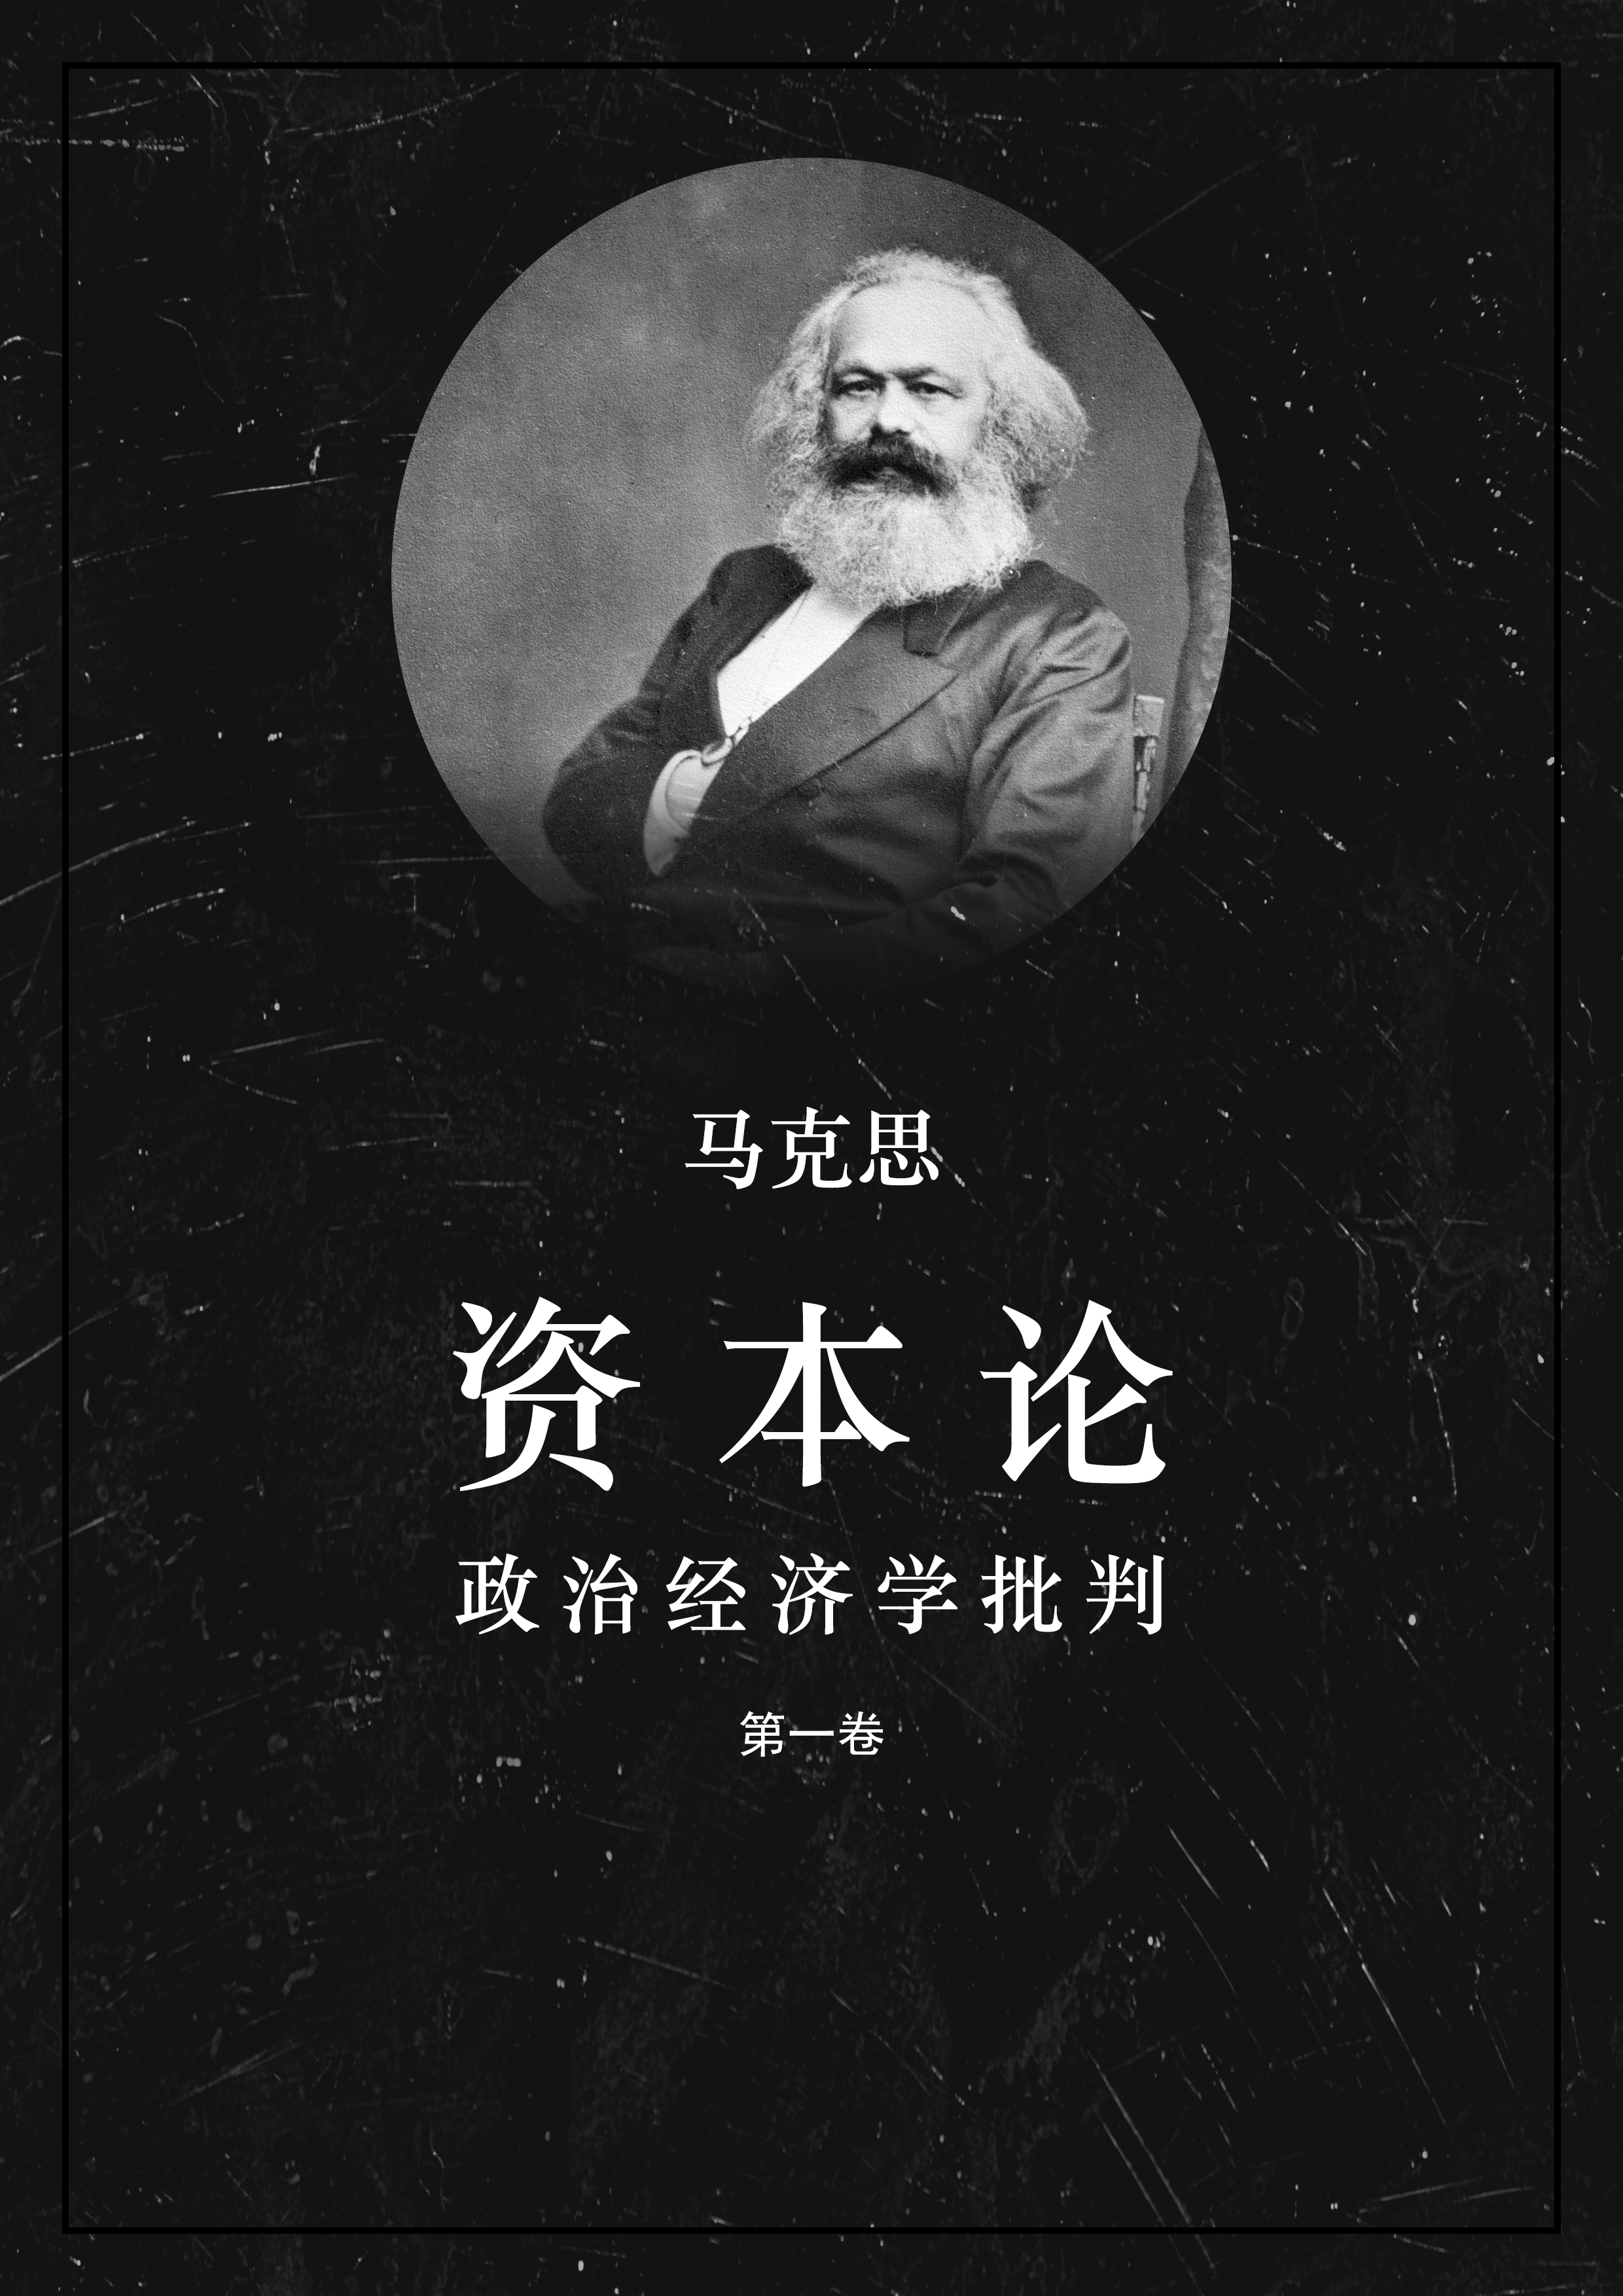
\includepdf[width=\paperwidth]{figures/资本论封面.png}
    \end{center}
\end{figure}

\thispagestyle{empty}
\clearpage

%————————————
%全世界无产者,联合起来!

\vspace*{\fill}
    \begin{center}
        \large{\textcolor{red}{全世界无产者,联合起来!}}
    \end{center}
\vspace*{\fill}

\thispagestyle{empty}

\newpage
\mbox{}
\thispagestyle{empty}
\clearpage
\newpage


%————————————


\vspace*{\fill}
    \begin{center}
        \zihao{0}{\textbf{第一卷\\资本的生产过程}}
    \end{center}
\vspace*{\fill}

\thispagestyle{empty}

\newpage
\mbox{}
\thispagestyle{empty}
\clearpage
\newpage




%————————————
% 目录

\setcounter{tocdepth}{5}% 设置目录级数
\setcounter{secnumdepth}{4}% 设置在几级目录前标记序号

\setcounter{page}{1}
\pagenumbering{Roman}

\tableofcontents

\clearpage

%————————————
%信

\vspace*{\fill}
    \begin{center}
        马克思1876年8月16日给恩格斯的信
    \end{center}
\vspace*{\fill}

\thispagestyle{empty}
\clearpage

%————
%信

\vspace*{\fill}
    \begin{center}
        \large{献\hspace{2em}给\\
        \texttt{我的不能忘记的朋友\\
        勇敢的忠实的高尚的无产阶级先锋战士}}\\
        \LARGE{威廉•沃尔弗}

        \normalsize{~\\ 

        1809年6月21日生于塔尔瑙\\
        1864年5月9日死于曼彻斯特流亡生活中}
    \end{center}
\vspace*{\fill}

\thispagestyle{empty}
\clearpage

%————————————
%序跋
\frontmatter

\chapter[卡尔·马克思\hspace{1em}第一版序言]{第一版序言\\{\small 卡尔·马克思}}

现在我把这部著作的第一卷交给读者。这部著作是我1859年发表的《政治经济学批判》的续篇。初篇和续篇相隔很久,是由于多年的疾病一再中断了我的工作。

前书的内容已经概述在这一卷的第一章中[2]。这样做不仅是为了联贯和完整,叙述方式也改进了。在情况许可的范围内,前书只是略略提到的许多论点,这里都作了进一步的阐述;相反地,前书已经详细阐述的论点,这里只略略提到。关于价值理论和货币理论的历史的部分,现在自然完全删去了。但是前书的读者可以在本书第一章的注释中,找到有关这两种理论的历史的新材料。

万事开头难,每门科学都是如此。所以本书第一章,特别是分析商品的部分,是最难理解的。其中对价值实体和价值量的分析,我已经尽可能地做到通俗易懂\footnote{这样做之所以更加必要,是因为甚至斐·拉萨尔著作中反对舒尔采-德里奇的部分,即他声称已经提出我对那些问题的阐述的“思想精髓”的部分[3],也包含着严重的误解。顺便说一下,斐·拉萨尔经济著作中所有一般的理论原理,如关于资本的历史性质、关于生产关系和生产方式之间的联系等等,几乎是逐字地——甚至包括我创造的术语——从我的作品中抄去的,而且没有说明出处,这样做显然是出于宣传上的考虑。我当然不是说他在细节上的论述和实际上的应用,这同我没有关系。}。以货币形式为其完成形态的价值形式,是极无内容和极其简单的。然而,两千多年来人类智慧在这方面进行探讨的努力,并未得到什么结果,而对更有内容和更复杂的形式的分析,却至少已接近于成功。为什么会这样呢?因为已经发育的身体比身体的细胞容易研究些。并且,分析经济形式,既不能用显微镜,也不能用化学试剂。二者都必须用抽象力来代替。而对资产阶级社会说来,劳动产品的商品形式,或者商品的价值形式,就是经济的细胞形式。在浅薄的人看来,分析这种形式好象是斤斤于一些琐事。这的确是琐事,但这是显微镜下的解剖所要做的那种琐事。

因此,除了价值形式那一部分外,不能说这本书难懂。当然,我指的是那些想学到一些新东西、因而愿意自己思考的读者。

物理学家是在自然过程表现得最确实、最少受干扰的地方考察自然过程的,或者,如有可能,是在保证过程以其纯粹形态进行的条件下从事实验的。我要在本书研究的,是资本主义生产方式以及和它相适应的生产关系和交换关系。到现在为止,这种生产方式的典型地点是英国。因此,我在理论阐述上主要用英国作为例证。但是,如果德国读者看到英国工农业工人所处的境况而伪善地耸耸肩膀,或者以德国的情况远不是那样坏而乐观地自我安慰,那我就要大声地对他说:这正是说的阁下的事情![4]

问题本身并不在于资本主义生产的自然规律所引起的社会对抗的发展程度的高低。问题在于这些规律本身,在于这些以铁的必然性发生作用并且正在实现的趋势。工业较发达的国家向工业较不发达的国家所显示的,只是后者未来的景象。

撇开这点不说。在资本主义生产已经在我们那里完全确立的地方,例如在真正的工厂里,由于没有起抗衡作用的工厂法,情况比英国要坏得多。在其他一切方面,我们也同西欧大陆所有其他国家一样,不仅苦于资本主义生产的发展,而且苦于资本主义生产的不发展。除了现代的灾难而外,压迫着我们的还有许多遗留下来的灾难,这些灾难的产生,是由于古老的陈旧的生产方式以及伴随着它们的过时的社会关系和政治关系还在苟延残喘。不仅活人使我们受苦,而且死人也使我们受苦。死人抓住活人!

德国和西欧大陆其他国家的社会统计,与英国相比是很贫乏的。然而它还是把帷幕稍稍揭开,使我们刚刚能够窥见幕内美杜莎的头。如果我国各邦政府和议会象英国那样,定期指派委员会去调查经济状况,如果这些委员会象英国那样,有全权去揭发真相,如果为此能够找到象英国工厂视察员、编写《公共卫生》报告的英国医生、调查女工童工受剥削的情况以及居住和营养条件等等的英国调查委员那样内行、公正、坚决的人们,那末,我国的情况就会使我们大吃一惊。柏修斯需要一顶隐身帽来追捕妖怪。我们却用隐身帽紧紧遮住眼睛和耳朵,以便有可能否认妖怪的存在。

决不要在这上面欺骗自己。正象十八世纪美国独立战争给欧洲中产阶级敲起了警钟一样,十九世纪美国南北战争又给欧洲工人阶级敲起了警钟。在英国,变革过程已经十分明显。它达到一定程度后,一定会波及大陆。在那里,它将采取较残酷的还是较人道的形式,那要看工人阶级自身的发展程度而定。所以,现在的统治阶级,不管有没有较高尚的动机,也不得不为了自己的切身利益,把一切可以由法律控制的、妨害工人阶级发展的障碍除去。因此,我在本卷中用了很大的篇幅来叙述英国工厂法的历史、内容和结果。一个国家应该而且可以向其他国家学习。一个社会即使探索到了本身运动的自然规律,——本书的最终目的就是揭示现代社会的经济运动规律,——它还是既不能跳过也不能用法令取消自然的发展阶段。但是它能缩短和减轻分娩的痛苦。

为了避免可能产生的误解,要说明一下。我决不用玫瑰色描绘资本家和地主的面貌。不过这里涉及到的人,只是经济范畴的人格化,是一定的阶级关系和利益的承担者。我的观点是:社会经济形态的发展是一种自然历史过程。不管个人在主观上怎样超脱各种关系,他在社会意义上总是这些关系的产物。同其他任何观点比起来,我的观点是更不能要个人对这些关系负责的。

在政治经济学领域内,自由的科学研究遇到的敌人,不只是它在一切其他领域内遇到的敌人。政治经济学所研究的材料的特殊性,把人们心中最激烈、最卑鄙、最恶劣的感情,把代表私人利益的复仇女神召唤到战场上来反对自由的科学研究。例如,英国高教会宁愿饶恕对它的三十九个信条中的三十八个信条展开的攻击,而不饶恕对它的现金收入的三十九分之一进行的攻击。在今天,同批评传统的财产关系相比,无神论本身是一种很轻的罪。但在这方面,进步仍然是无可怀疑的。以最近几星期内发表的蓝皮书[5]《关于工业和工联问题同女王陛下驻外公使馆的通讯》为例。英国女王驻外使节在那里坦率地说,在德国,在法国,一句话,在欧洲大陆的一切文明国家,现有的劳资关系的变革同英国一样明显,一样不可避免。同时,大西洋彼岸的美国副总统威德先生也在公众集会上说:在奴隶制废除后,资本关系和土地所有权关系的变革会提到日程上来!这是时代的标志,不是用紫衣黑袍遮掩得了的。这并不是说明天就会出现奇迹。但这表明,甚至在统治阶级中间也已经透露出一种模糊的感觉:现在的社会不是坚实的结晶体,而是一个能够变化并且经常处于变化过程中的机体。

这部著作的第二卷将探讨资本的流通过程(第二册)和总过程的各种形式(第三册),第三卷即最后一卷(第四册)将探讨理论史。

任何的科学批评的意见我都是欢迎的。而对于我从来就不让步的所谓舆论的偏见,我仍然遵守伟大的佛罗伦萨诗人的格言:

走你的路,让人们去说罢![6]

\begin{flushright}
    \textbf{卡尔·马克思}\\
    \small{1867年7月25日于伦敦}
\end{flushright}



\chapter[卡尔·马克思\hspace{1em}第二版跋]{第二版跋\\{\small 卡尔·马克思}}

我首先应当向第一版的读者指出第二版中所作的修改。很明显的是,篇目更加分明了。各处新加的注,都标明是第二版注。就正文说,最重要的有下列各点:

第一章第一节更加科学而严密地从表现每个交换价值的等式的分析中引出了价值,而且明确地突出了在第一版中只是略略提到的价值实体和由社会必要劳动时间决定的价值量之间的联系。第一章第三节(价值形式)全部改写了,第一版的双重叙述就要求这样做。——顺便指出,这种双重叙述是我的朋友,汉诺威的路·库格曼医生建议的。1867年春,初校样由汉堡寄来时,我正好访问他。他劝我说,大多数读者需要有一个关于价值形式的更带讲义性的补充说明。——第一章最后一节《商品的拜物教性质及其秘密》大部分修改了。第三章第一节(价值尺度)作了详细的修改,因为在第一版中,考虑到《政治经济学批判》(1859年柏林版)已有的说明,这一节是写得不够细致的。第七章,特别是这一章的第二节,作了很大的修改。

原文中局部的、往往只是修辞上的修改,用不着一一列举出来。这些修改全书各处都有。但是,现在我校阅要在巴黎出版的法译本时,发现德文原本某些部分需要更彻底地修改,某些部分需要更好地修辞或更仔细地消除一些偶然的疏忽。可是我没有时间这样做,因为只是在1871年秋,正当我忙于其他迫切的工作的时候,我才接到通知说,书已经卖完了,而第二版在1872年1月就要付印。

《资本论》在德国工人阶级广大范围内迅速得到理解,是对我的劳动的最好的报酬。一个在经济方面站在资产阶级立场上的人,维也纳的工厂主迈尔先生,在普法战争期间发行的一本小册子中[7]说得很对:被认为是德国世袭财产的卓越的理论思维能力,已在德国的所谓有教养的阶级中完全消失了,但在德国工人阶级中复活了。[8]

在德国,直到现在,政治经济学一直是外来的科学。古斯达夫·冯·居利希在他的《商业、工业和农业的历史叙述》中,特别是在1830年出版的该书的前两卷中,已经大体上谈到了妨碍我国资本主义生产方式发展、因而也妨碍我国现代资产阶级社会建立的历史条件。可见,政治经济学在我国缺乏生存的基础。它作为成品从英国和法国输入;德国的政治经济学教授一直是学生。别国的现实在理论上的表现,在他们手中变成了教条集成,被他们用包围着他们的小资产阶级世界的精神去解释,就是说,被曲解了。他们不能把在科学上无能为力的感觉完全压制下去,他们不安地意识到,他们必须在一个实际上不熟悉的领域内充当先生,于是就企图用博通文史的美装,或用无关材料的混合物来加以掩饰。这种材料是从所谓官房学——各种知识的杂拌,满怀希望的\footnote{第3版和第4版中是:毫无希望的。——编者注}德国官僚候补者必须通过的炼狱之火——抄袭来的。

从1848年起,资本主义生产在德国迅速地发展起来,现在正是它的欺诈盛行的时期。但是我们的专家还是命运不好。当他们能够公正无私地研究政治经济学时,在德国的现实中没有现代的经济关系。而当这种关系出现时,他们所处的境况已经不再容许他们在资产阶级的视野之内进行公正无私的研究了。只要政治经济学是资产阶级的政治经济学,就是说,只要它把资本主义制度不是看作历史上过渡的发展阶段,而是看作社会生产的绝对的最后的形式,那就只有在阶级斗争处于潜伏状态或只是在个别的现象上表现出来的时候,它还能够是科学。

拿英国来说。英国古典政治经济学是属于阶级斗争不发展的时期的。它的最后的伟大的代表李嘉图,终于有意识地把阶级利益的对立、工资和利润的对立、利润和地租的对立当作他的研究的出发点,因为他天真地把这种对立看作社会的自然规律。这样,资产阶级的经济科学也就达到了它的不可逾越的界限。还在李嘉图活着的时候,就有一个和他对立的人西斯蒙第批判资产阶级的经济科学了。\footnote{见我的《政治经济学批判》第39页[9]。}

随后一个时期,从1820年到1830年,在英国,政治经济学方面的科学活动极为活跃。这是李嘉图的理论庸俗化和传播的时期,同时也是他的理论同旧的学派进行斗争的时期。这是一场出色的比赛。当时的情况,欧洲大陆知道得很少,因为论战大部分是分散在杂志论文、关于时事问题的著作和抨击性小册子上。这一论战的公正无私的性质——虽然李嘉图的理论也例外地被用作攻击资产阶级经济的武器——可由当时的情况来说明。一方面,大工业刚刚脱离幼年时期;大工业只是从1825年的危机才开始它的现代生活的周期循环,就证明了这一点。另一方面,资本和劳动之间的阶级斗争被推到后面:在政治方面是由于纠合在神圣同盟周围的政府和封建主同资产阶级所领导的人民大众之间发生了纠纷;在经济方面是由于工业资本和贵族土地所有权之间发生了纷争。这种纷争在法国是隐藏在小块土地所有制和大土地所有制的对立后面,在英国则在谷物法颁布后公开爆发出来。这个时期英国的政治经济学文献,使人想起魁奈医生逝世后法国经济学的狂飙时期,但这只是象晚秋晴日使人想起春天一样。1830年,最终决定一切的危机发生了。

法国和英国的资产阶级夺得了政权。从那时起,阶级斗争在实践方面和理论方面采取了日益鲜明的和带有威胁性的形式。它敲响了科学的资产阶级经济学的丧钟。现在问题不再是这个或那个原理是否正确,而是它对资本有利还是有害,方便还是不方便,违背警章还是不违背警章。不偏不倚的研究让位于豢养的文丐的争斗,公正无私的科学探讨让位于辩护士的坏心恶意。甚至以工厂主科布顿和布莱特为首的反谷物法同盟[10]抛出的强迫人接受的小册子,由于对地主贵族展开了论战,即使没有科学的意义,毕竟也有历史的意义。但是从罗伯特·皮尔爵士执政以来,这最后一根刺也被自由贸易的立法从庸俗经济学那里拔掉了。

1848年大陆的革命也在英国产生了反应。那些还要求有科学地位、不愿单纯充当统治阶级的诡辩家和献媚者的人,力图使资本的政治经济学同这时已不容忽视的无产阶级的要求调和起来。于是,以约翰·斯图亚特·穆勒为最著名代表的毫无生气的混合主义产生了。这宣告了“资产阶级”经济学的破产,关于这一点,俄国的伟大学者和批评家尼·车尔尼雪夫斯基在他的《穆勒政治经济学概述》中已作了出色的说明。

可见,在资本主义生产方式的对抗性质在法英两国通过历史斗争而明显地暴露出来以后,资本主义生产方式才在德国成熟起来,同时,德国无产阶级比德国资产阶级在理论上已经有了更明确的阶级意识。因此,当资产阶级政治经济学作为一门科学看来在德国有可能产生的时候,它又成为不可能了。

在这种情况下,资产阶级政治经济学的代表人物分成了两派。一派是精明的、贪利的实践家,他们聚集在庸俗经济学辩护论的最浅薄的因而也是最成功的代表巴师夏的旗帜下。另一派是以经济学教授资望自负的人,他们追随约·斯·穆勒,企图调和不能调和的东西。德国人在资产阶级经济学衰落时期,也同在它的古典时期一样,始终只是学生、盲从者和模仿者,是外国大商行的小贩。

所以,德国社会特殊的历史发展,排除了“资产阶级”经济学在德国取得任何独创的成就的可能性,但是没有排除对它进行批判的可能性。就这种批判代表一个阶级而论,它能代表的只是这样一个阶级,这个阶级的历史使命是推翻资本主义生产方式和最后消灭阶级。这个阶级就是无产阶级。

德国资产阶级的博学的和不学无术的代言人,最初企图象他们在对付我以前的著作时曾经得逞那样,用沉默置《资本论》于死地。当这种策略已经不再适合时势的时候,他们就借口批评我的书,开了一些单方来“镇静资产阶级的意识”,但是他们在工人报刊上(例如约瑟夫·狄慈根在《人民国家报》上发表的文章[11])遇到了强有力的对手,至今还没有对这些对手作出答复。\footnote{德国庸俗经济学的油嘴滑舌的空谈家,指责我的著作的文体和叙述方法。没有人会比我本人更严厉地评论《资本论》的文字上的缺点。然而,为了使这些先生及其读者受益和愉快,我要在这里援引一篇英国的和一篇俄国的评论。同我的观点完全敌对的《星期六评论》在其关于德文第一版的短评中说道:叙述方法“使最枯燥无味的经济问题具有一种独特的魅力”。1872年4月20日的《圣彼得堡消息报》也说:“除了少数太专门的部分以外,叙述的特点是通俗易懂,明确,尽管研究对象的科学水平很高却非常生动。在这方面,作者……和大多数德国学者大不相同,这些学者……用含糊不清、枯燥无味的语言写书,以致普通人看了脑袋都要裂开。”但是,对现代德国民族主义自由主义教授的著作的读者说来,要裂开的是和脑袋完全不同的东西。}

1872年春,彼得堡出版了《资本论》的优秀的俄译本。初版三千册现在几乎已售卖一空。1871年,基辅大学政治经济学教授尼·季别尔先生在他的《李嘉图的价值和资本的理论》一书中就已经证明,我的价值、货币和资本的理论就其要点来说是斯密—李嘉图学说的必然的发展。使西欧读者在阅读他的这本出色的著作时感到惊异的,是纯理论观点的始终一贯。
人们对《资本论》中应用的方法理解得很差,这已经由各种互相矛盾的评论所证明。

例如,巴黎的《实证论者评论》[12]一方面责备我形而上学地研究经济学,另一方面责备我——你们猜猜看!——只限于批判地分析既成的事实,而没有为未来的食堂开出调味单(孔德主义的吗?)。关于形而上学的责备,季别尔教授指出:

\texttt{“就理论本身来说,马克思的方法是整个英国学派的演绎法,其优点和缺点是一切最优秀的理论经济学家所共有的。”}

莫·布洛克先生在《德国的社会主义理论家》(摘自1872年7月和8月《经济学家杂志》)一文中,指出我的方法是分析的方法,他说:

\texttt{“马克思先生通过这部著作而成为一个最出色的具有分析能力的思想家”。}

德国的评论家当然大叫什么黑格尔的诡辩。彼得堡的《欧洲通报》在专谈《资本论》的方法一文(1872年5月号第427—436页[14])中,认为我的研究方法是严格的现实主义的,而叙述方法不幸是德国辩证法的。作者写道:

\texttt{“如果从外表的叙述形式来判断,那末最初看来,马克思是最大的唯心主义哲学家,而且是德国的即坏的唯心主义哲学家。而实际上,在经济学的批判方面,他是他的所有前辈都无法比拟的现实主义者……决不能把他称为唯心主义者。”}

我回答这位作者先生的最好的办法,是从他自己的批评中摘出几段话来,这几段话也会使某些不懂俄文原文的读者感到兴趣。

这位作者先生从我的《政治经济学批判》序言(1859年柏林版第4—7页[15],在那里我说明了我的方法的唯物主义基础)中摘引一段话后说:

\texttt{“在马克思看来,只有一件事情是重要的,那就是发现他所研究的那些现象的规律。而且他认为重要的,不仅是在这些现象具有完成形式和处于一定时期内可见到的联系中的时候支配着它们的那种规律。在他看来,除此而外,最重要的是这些现象变化的规律,这些现象发展的规律,即它们由一种形式过渡到另一种形式,由一种联系秩序过渡到另一种联系秩序的规律。他一发现了这个规律,就详细地来考察这个规律在社会生活中表现出来的各种后果……所以马克思竭力去做的只是一件事:通过准确的科学研究来证明一定的社会关系秩序的必然性,同时尽可能完善地指出那些作为他的出发点和根据的事实。为了这个目的,只要证明现有秩序的必然性,同时证明这种秩序不可避免地要过渡到另一种秩序的必然性就完全够了,而不管人们相信或不相信,意识到或没有意识到这种过渡。马克思把社会运动看作受一定规律支配的自然历史过程,这些规律不仅不以人的意志、意识和意图为转移,反而决定人的意志、意识和意图……既然意识要素在文化史上只起着这种从属作用,那末不言而喻,以文化本身为对象的批判,比任何事情更不能以意识的某种形式或某种结果为依据。这就是说,作为这种批判的出发点的不能是观念,而只能是外部的现象。批判将不是把事实和观念比较对照,而是把一种事实同另一种事实比较对照。对这种批判唯一重要的是,把两种事实尽量准确地研究清楚,使之真正形成相互不同的发展阶段,但尤其重要的是,同样准确地把各种秩序的序列、把这些发展阶段所表现出来的联贯性和联系研究清楚……但是有人会说,经济生活的一般规律,不管是应用于现在或过去,都是一样的。马克思否认的正是这一点。在他看来,这样的抽象规律是不存在的……根据他的意见,恰恰相反,每个历史时期都有它自己的规律。一旦生活经过了一定的发展时期,由一定阶段进入另一阶段时,它就开始受另外的规律支配。总之,经济生活呈现出的现象,和生物学的其他领域的发展史颇相类似……旧经济学家不懂得经济规律的性质,他们把经济规律同物理学定律和化学定律相比拟……对现象所作的更深刻的分析证明,各种社会机体象动植物机体一样,彼此根本不同……由于各种机体的整个结构不同,它们的各个器官有差别,以及器官借以发生作用的条件不一样等等,同一个现象却受完全不同的规律支配。例如,马克思否认人口规律在任何时候在任何地方都是一样的。相反地,他断言每个发展阶段有它自己的人口规律……生产力的发展水平不同,生产关系和支配生产关系的规律也就不同。马克思给自己提出的目的是,从这个观点出发去研究和说明资本主义经济制度,这样,他只不过是极其科学地表述了任何对经济生活进行准确的研究必须具有的目的……这种研究的科学价值在于阐明了支配着一定社会机体的产生、生存、发展和死亡以及为另一更高的机体所代替的特殊规律。马克思的这本书确实具有这种价值”。}

这位作者先生把他称为我的实际方法的东西描述得这样恰当,并且在考察我个人对这种方法的运用时又抱着这样的好感,那他所描述的不正是辩证方法吗?

当然,在形式上,叙述方法必须与研究方法不同。研究必须充分地占有材料,分析它的各种发展形式,探寻这些形式的内在联系。只有这项工作完成以后,现实的运动才能适当地叙述出来。这点一旦做到,材料的生命一旦观念地反映出来,呈现在我们面前的就好象是一个先验的结构了。
我的辩证方法,从根本上来说,不仅和黑格尔的辩证方法不同,而且和它截然相反。在黑格尔看来,思维过程,即他称为观念而甚至把它变成独立主体的思维过程,是现实事物的创造主,而现实事物只是思维过程的外部表现。我的看法则相反,观念的东西不外是移入人的头脑并在人的头脑中改造过的物质的东西而已。

将近三十年以前,当黑格尔辩证法还很流行的时候,我就批判过黑格尔辩证法的神秘方面。但是,正当我写《资本论》第一卷时,愤懑的、自负的、平庸的、今天在德国知识界发号施令的模仿者们[16],却已高兴地象莱辛时代大胆的莫泽斯·门德尔森对待斯宾诺莎那样对待黑格尔,即把他当作一条“死狗”了。因此,我要公开承认我是这位大思想家的学生,并且在关于价值理论的一章中,有些地方我甚至卖弄起黑格尔特有的表达方式。辩证法在黑格尔手中神秘化了,但这决不妨碍他第一个全面地有意识地叙述了辩证法的一般运动形式。在他那里,辩证法是倒立着的。必须把它倒过来,以便发现神秘外壳中的合理内核。

辩证法,在其神秘形式上,成了德国的时髦东西,因为它似乎使现存事物显得光彩。辩证法,在其合理形态上,引起资产阶级及其夸夸其谈的代言人的恼怒和恐怖,因为辩证法在对现存事物的肯定的理解中同时包含对现存事物的否定的理解,即对现存事物的必然灭亡的理解;辩证法对每一种既成的形式都是从不断的运动中,因而也是从它的暂时性方面去理解;辩证法不崇拜任何东西,按其本质来说,它是批判的和革命的。

使实际的资产者最深切地感到资本主义社会充满矛盾的运动的,是现代工业所经历的周期循环的变动,而这种变动的顶点就是普遍危机。这个危机又要临头了,虽然它还处于预备阶段;由于它的舞台的广阔和它的作用的强烈,它甚至会把辩证法灌进新的神圣普鲁士德意志帝国的暴发户们的头脑里去。

\begin{flushright}
    \textbf{卡尔·马克思}\\
    \small{1873年1月24日于伦敦}
\end{flushright}






\chapter[卡尔·马克思\hspace{1em}法文版序言]{法文版序言\\{\small 卡尔·马克思}}

致莫里斯·拉沙特尔公民

亲爱的公民:

您想定期分册出版《资本论》的译本,我很赞同。这本书这样出版,更容易到达工人阶级的手里,在我看来,这种考虑是最为重要的。

这是您的想法好的一面,但也有坏的一面:我所使用的分析方法至今还没有人在经济问题上运用过,这就使前几章读起来相当困难。法国人总是急于追求结论,渴望知道一般原则同他们直接关心的问题的联系,因此我很担心,他们会因为一开始就不能继续读下去而气馁。

这是一种不利,对此我没有别的办法,只有事先向追求真理的读者指出这一点,并提醒他们。在科学上没有平坦的大道,只有不畏劳苦沿着陡峭山路攀登的人,才有希望达到光辉的顶点。
亲爱的公民,请接受我对您的忠诚。

\begin{flushright}
    \textbf{卡尔·马克思}\\
    \small{1872年3月18日于伦敦}
\end{flushright}


\chapter[卡尔·马克思\hspace{1em}法文版跋]{法文版跋\\{\small 卡尔·马克思}}

约·鲁瓦先生保证尽可能准确地、甚至逐字逐句地进行翻译。他非常认真地完成了自己的任务。但正因为他那样认真,我不得不对表述方法作些修改,使读者更容易理解。由于本书分册出版,这些修改是逐日作的,所以不能处处一样仔细,文体不免有不一致的地方。

在担负校正工作后,我就感到作为依据的原本(德文第二版)应当作一些修改,有些论述要简化,另一些要加以完善,一些补充的历史材料或统计材料要加进去,一些批判性评注要增加,等等。不管这个法文版本有怎样的文字上的缺点,它仍然在原本之外有独立的科学价值,甚至对懂德语的读者也有参考价值。

下面是我从德文第二版跋中摘引的几段,是有关政治经济学在德国的发展和本书运用的方法的。

\begin{flushright}
    \textbf{卡尔·马克思}\\
    \small{1875年4月28日于伦敦}
\end{flushright}


\chapter[弗里德里希·恩格斯\hspace{1em}第三版序言]{第三版序言\\{\small 弗里德里希·恩格斯}}

马克思不幸已不能亲自进行这个第三版的付印准备工作。这位大思想家——现在,连反对他的人也拜服他的伟大了——已于1883年3月14日逝世。

我失去了一个相交四十年的最好的、最亲密的朋友,他给我的教益是无法用言语形容的。现在,不论出版这个第三版的任务,还是出版以手稿形式遗留下来的第二卷的任务,都落在我的身上了。在这里,我应该告诉读者,我是怎样履行前一项任务的。

马克思原想把第一卷原文大部分改写一下,把某些论点表达得更明确一些,把新的论点增添进去,把直到最近时期的历史材料和统计材料补充进去。由于他的病情和急于完成第二卷的定稿,他放弃了这一想法。他只作了一些最必要的修改,只把当时出版的法文版[17]中已有的增补收了进去。

在马克思的遗物中,我发现了一个德文本,其中有些地方他作了修改,标明何处应参看法文版;同时还发现了一个法文本,其中准确地标出了所要采用的地方。这些修改和增补,除少数外,都属于本书的最后一部分,即资本的积累过程那一篇。旧版的这一篇原文比其他各篇更接近于初稿,而前面各篇都作过比较彻底的修改。因此,这一篇的文体更加生动活泼,更加一气呵成,但也更不讲究,夹杂英文语气,有不明确的地方;叙述过程中间或有不足之处,因为个别重要论点只是提了一下。

说到文体,马克思亲自彻底校订了许多章节,并且多次作过口头指示,这就给了我一个标准去取舍英文术语和英文语气。马克思一定还会修改那些增补的地方,并且用他那精练的德语代替流畅的法语;而我只要把它们移译过来,尽量和原文协调一致,也就满足了。

因此,在这第三版中,凡是我不能确定作者自己是否会修改的地方,我一个字也没有改。我也没有想到把德国经济学家惯用的一些行话弄到《资本论》里面来。例如,这样一种费解的行话:把通过支付现金而让别人为自己劳动的人叫做劳动给予者,把为了工资而让别人取走自己的劳动的人叫做劳动受取者。法文travail〔劳动〕在日常生活中也有“职业”的意思。但是,如果有个经济学家把资本家叫做donneur de travail〔劳动给予者〕,把工人叫做receveur de travail〔劳动受取者〕,法国人当然会把他看作疯子。

我也不能把原文中到处使用的英制货币和度量衡单位换算成新德制单位。在第一版出版时,德制度量衡种类之多,犹如一年的天数那样,马克有两种(帝国马克当时还只存在于泽特贝尔的头脑中,这是他在三十年代末发明的),古尔登有两种,塔勒至少有三种,其中一种以“新三分之二”[18]为单位。在自然科学上通用的是公制度量衡,在世界市场上通用的是英制度量衡。在这种情况下,对于一部几乎完全要从英国的工业状况中取得实际例证的著作来说,采用英制计量单位是很自然的。这后一种理由直到今天还有决定意义,尤其因为世界市场上的有关情况几乎没有什么变化,而且正是在那些有决定意义的工业部门——制铁业和棉纺织业,至今通用的还几乎完全是英制度量衡。

最后,我说几句关于马克思的不大为人们了解的引证方法。在单纯叙述和描写事实的地方,引文(例如引用英国蓝皮书)自然是作为简单的例证。而在引证其他经济学家的理论观点的地方,情况就不同了。这种引证只是为了确定:一种在发展过程中产生的经济思想,是什么地方、什么时候、什么人第一次明确地提出的。这里考虑的只是,所提到的经济见解在科学史上是有意义的,能够多少恰当地从理论上表现当时的经济状况。至于这种见解从作者的观点来看是否还有绝对的或相对的意义,或者完全成为历史上的东西,那是毫无关系的。因此,这些引证只是从经济科学的历史中摘引下来作为正文的注解,从时间和首倡者两方面说明经济理论中各个比较重要的成就。这种工作在这样一种科学上是很必要的,这种科学的历史著作家们一直只是以怀有偏见、不学无术、追名逐利而著称。——现在我们也会明白,和第二版跋中所说的情况一样,为什么马克思只是在极例外的场合才引证德国经济学家的言论。

第二卷可望在1884年出版。

\begin{flushright}
    \textbf{弗里德里希·恩格斯}\\
    \small{1883年11月7日于伦敦}
\end{flushright}

\chapter[弗里德里希·恩格斯\hspace{1em}英文版序言]{英文版序言\\{\small 弗里德里希·恩格斯}}

关于《资本论》英译本的出版,不需要作任何解释了。但是鉴于本书阐述的理论几年前就已经为英美两国的定期刊物和现代著作经常提到,被攻击或辩护,被解释或歪曲,倒是需要说明一下为什么这个英译本延迟到今天才出版。

作者于1883年逝世后不久,我们就明显地感到这部著作确实需要一个英文版本,当时赛米尔·穆尔先生(马克思和本文作者多年的朋友,他可能比任何人都更熟悉这部著作)同意担任马克思的遗著处理人迫切希望出版的英译本的翻译工作。我们商定,由我对照原文校订译稿,并且在我认为适当的地方提出修改意见。但是后来,我们看到,穆尔先生本身的业务使他不能如我们大家所期待的那样很快完成翻译工作,于是我们欣然接受了艾威林博士的建议,由他担任一部分翻译工作。同时,马克思的小女儿艾威林夫人建议,由她核对引文,把引自英国作者和蓝皮书并由马克思译成德文的许多文句恢复成原文。除了少数无法避免的例外,她全部完成了这项工作。

本书下述各部分是艾威林博士翻译的:1.第十章(工作日)和第十一章(剩余价值率和剩余价值量);2.第六篇(工资,包括第十九章至第二十二章);3.第二十四章第四节(决定积累量的情况)至本书结尾,包括第二十四章最后一部分,第二十五章和第八篇全部(第二十六章至第三十三章);4.作者的两篇序言[19]。其余部分全是穆尔先生翻译的。因此,译者只对各自的译文负责,而我对整个工作负全部责任。

我们全部译文所依据的德文第三版,是我在1883年利用作者遗留的笔记整理的,笔记注明第二版的哪些地方应当改成1873年法文版标出的文句\footnote{《资本论》,卡尔·马克思著,莫·约·鲁瓦译,全文由作者校阅,由拉沙特尔在巴黎出版。这个译本,特别是该书的最后一部分,对德文第2版作了相当多的修改和补充。}。第二版原文中这样修改的地方,和马克思曾经为一个英译本(大约十年前在美国有人打算出版的一个英译本,但主要由于没有十分合适的译者而作罢)所写的许多书面指示中提出需要修改的地方大体相同。这份手稿是由我们的老朋友,新泽西州霍布根的弗·阿·左尔格提供给我们的。手稿指出,还有一些地方应该按照法文版进行补充;但是因为这份手稿是早在马克思对第三版作最后指示的前几年写的,所以我不敢随便利用它,除非在个别情况下,并且主要是在它有助于我们解决某些疑难问题的情况下才加以利用。而大多数有疑难问题的句子,我们也参考了法文本,因为它指出了,原文中某些有意义而在翻译中不得不舍弃的地方,作者自己也是打算舍弃的。

可是,有一个困难是我们无法为读者解除的。这就是:某些术语的应用,不仅同它们在日常生活中的含义不同,而且和它们在普通政治经济学中的含义也不同。但这是不可避免的。一门科学提出的每一种新见解,都包含着这门科学的术语的革命。化学是最好的例证,它的全部术语大约每二十年就彻底变换一次,几乎很难找到一种有机化合物不是先后拥有一系列不同的名称的。政治经济学通常满足于照搬工商业生活上的术语并运用这些术语,完全看不到这样做会使自己局限于这些术语所表达的观念的狭小范围。例如,古典政治经济学虽然完全知道,利润和地租都不过是工人必须向自己雇主提供的产品中无酬部分(雇主是这部分产品的第一个占有者,但不是它的最后的唯一的所有者)的一部分、一份,但即使这样,它也从来没有超出通常关于利润和地租的概念,从来没有把产品中这个无酬部分(马克思称它为剩余产品),就其总和即当作一个整体来研究过,因此,也从来没有对它的起源和性质,对制约着它的价值的以后分配的那些规律有一个清楚的理解。同样,一切产业,除了农业和手工业以外,都一概被包括在制造业(manufacture)这个术语中,这样,经济史上两个重大的本质不同的时期即以手工分工为基础的真正工场手工业时期和以使用机器为基础的现代工业时期的区别,就被抹杀了。不言而喻,把现代资本主义生产只看作是人类经济史上一个暂时阶段的理论所使用的术语,和把这种生产形式看作是永恒的最终阶段的那些作者所惯用的术语,必然是不同的。

关于作者的引证方法,不妨说几句。在大多数场合,也和往常一样,引文是用作证实文中论断的确凿证据。但在不少场合,引证经济学著作家的文句是为了证明:什么时候、什么地方、什么人第一次明确地提出某一观点。只要引用的论点具有重要意义,能够多少恰当地表现某一时期占统治地位的社会生产和交换条件,马克思就加以引证,至于马克思是否承认这种论点,或者说,这种论点是否具有普遍意义,那是完全没有关系的。因此,这些引证是从科学史上摘引下来并作为注解以充实正文的。

我们这个译本只包括这部著作的第一卷。但这第一卷是一部相当完整的著作,并且二十年来一直被当作一部独立的著作。1885年我用德文出版的第二卷,由于没有第三卷,显然是不完全的,而第三卷在1887年年底以前不能出版。到第三卷德文原稿刊行时,再考虑准备第二、三两卷的英文版也为时不晚。

《资本论》在大陆上常常被称为“工人阶级的圣经”。任何一个熟悉工人运动的人都不会否认:本书所作的结论日益成为伟大的工人阶级运动的基本原则,不仅在德国和瑞士是这样,而且在法国,在荷兰和比利时,在美国,甚至在意大利和西班牙也是这样;各地的工人阶级都越来越把这些结论看成是对自己的状况和自己的期望所作的最真切的表述。而在英国,马克思的理论正是在目前对社会主义运动产生着巨大的影响,这个运动在“有教养者”队伍中的传播,不亚于在工人阶级队伍中的传播。但这并不是一切。彻底研究英国的经济状况成为国民的迫切需要的时刻,很快就会到来。这个国家的工业体系的运动,——没有生产的从而没有市场的经常而迅速的扩大,这种运动就不可能进行,——已趋于停滞。自由贸易已经无计可施了;甚至曼彻斯特对自己这个昔日的经济福音也发生了怀疑[20]。迅速发展的外国工业,到处直接威胁着英国的生产,不仅在受关税保护的市场上,而且在中立市场上,甚至在英吉利海峡的此岸都是这样。生产力按几何级数增长,而市场最多也只是按算术级数扩大。1825年至1867年每十年反复一次的停滞、繁荣、生产过剩和危机的周期,看来确实已经结束,但这只是使我们陷入无止境的经常萧条的绝望泥潭。人们憧憬的繁荣时期将不再来临;每当我们似乎看到繁荣时期行将到来的种种预兆,这些预兆又消失了。而每一个冬天的来临都重新提出这一重大问题:“怎样对待失业者”;虽然失业人数年复一年地增加,却没有人解答这个问题;失业者再也忍受不下去,而要起来掌握自己命运的时刻,几乎指日可待了。毫无疑问,在这样的时刻,应当倾听这样一个人的声音,这个人的全部理论是他毕生研究英国的经济史和经济状况的结果,他从这种研究中得出这样的结论:至少在欧洲,英国是唯一可以完全通过和平的和合法的手段来实现不可避免的社会革命的国家。当然,他从来没有忘记附上一句话:他并不指望英国的统治阶级会不经过“维护奴隶制的叛乱”[21]而屈服在这种和平的和合法的革命面前。

\begin{flushright}
    \textbf{弗里德里希·恩格斯}\\
    \small{1886年11月5日}
\end{flushright}


\chapter[弗里德里希·恩格斯\hspace{1em}第四版序言]{第四版序言\\{\small 弗里德里希·恩格斯}}

第四版要求我尽可能把正文和注解最后确定下来。我是怎样实现这一要求的,可以简单说明如下:

根据再一次对照法文版和根据马克思亲手写的笔记,我又把法文版的一些地方补充到德文原文中去。这些补充是在第80页(第3版第88页)、第458—460页(第3版第509—510页)、第547—551页(第3版第600页)、第591—593页(第3版第644页)和第596页(第3版第648页)注79\footnote{见本卷第136、540-542、640-644、687-689、692-693页。——编者注。}。此外,我还按照法文版和英文版把一个很长的关于矿工的注解(第3版第509—515页)移入正文(第4版第461—467页)\footnote{见本卷第542-549页。——编者注}。其他一些小改动都是纯技术性的。

其次,我还补加了一些说明性的注释,特别是在那些由于历史情况的改变看来需要加注的地方。所有这些补加的注释都括在四角括号里,并且注有我的姓名的第一个字母或《D. H.》。\footnote{本卷括在花括号{}里,并注有弗·恩·。——编者注}

最近出版英文版时,曾对许多引文作了全面的校订,这是很必要的。马克思的小女儿爱琳娜不辞劳苦,对所有引文的原文都进行了核对,使占引文绝大多数的英文引文不再是德文的转译,而是它原来的英文原文。因此,在出第四版时,我必须参考这个恢复了原文的版本。在参考中发现了某些细小的不确切的地方:有的引文页码弄错了(这一部分是由于从笔记本上转抄时抄错了,一部分是由于前三版堆积下来的排印的错误);有的引号和省略号放错了位置(从札记本上抄录这么多的引文,这种差错是不可避免的);还有某些引文在翻译时用字不很恰当。有一些引文是根据马克思在1843—1845年在巴黎记的旧笔记本抄录的,当时马克思还不懂英语,他读英国经济学家的著作是读的法译本;那些经过两次转译的引文多少有些走了原意——如引自斯图亚特、尤尔等人著作的话就是如此。这些地方我都改以英文原文为根据。其他一些细小的不确切和疏忽的地方也都改正了。把第四版和以前各版对照一下,读者就会看出,所有这些细微的改正,并没有使本书的内容有丝毫值得一提的改变。只有一段引文没有找到出处,这就是理查·琼斯的一段话(第4版第562页注47\footnote{见本卷第656页。——编者注});多半是马克思把书名写错了[21]。所有其余的引文都仍然具有充分的说服力,甚至由于现在更加确切而更加具有说服力了。

不过,在此我不得不回溯一段往事。

据我所知,马克思的引文的正确性只有一次被人怀疑过。由于马克思逝世后这段引文的事又被重新提起,所以我不能不讲一讲。[22]

1872年3月7日,德国工厂主联盟的机关刊物柏林《协和》杂志刊登了一篇匿名作者的文章,标题是《卡尔·马克思是怎样引证的》。这篇文章的作者义愤填膺、粗暴无礼地指责马克思歪曲地引证了格莱斯顿1863年4月16日预算演说中的话(这句话引用在1864年国际工人协会成立宣言[23]中,并且在《资本论》第1卷第4版第617页即第3版第670—671页\footnote{见本卷第715页。——编者注}上再次引用)。这句话就是:“财富和实力这样令人陶醉的增长……完全限于有产阶级。”这篇文章的作者说,在《汉萨德》的(准官方的)速记记录中根本没有马克思引的这句话。“但是在格莱斯顿的演说中根本没有这句话。他在演说中说的和这句话正好相反。〈接着是黑体字〉\footnote{本卷引文中凡是尖括号〈 〉内的话或标点符号都是马克思或恩格斯加的。——译者注}\textbf{马克思在形式上和实质上增添了这句话!”}

马克思在5月接到了这一期《协和》杂志,他在6月1日的《人民国家报》上回答了这个匿名作者。由于当时他已记不起这一句话是引自哪一家报纸的报道,所以只得从两种英文出版物中举出意思完全相同的这句话,接着他引用了《泰晤士报》的报道。根据这一报道,格莱斯顿说:

\texttt{“从财富的观点来看,这个国家的状况就是这样。我应当承认,我几乎会怀着忧虑和悲痛的心情来看待财富和实力这样令人陶醉的增长,如果我相信,这种增长仅限于富裕阶级的话。这里完全没有注意到工人居民的状况。我刚刚描述的增长,亦即以我认为十分确切的材料为根据的增长,完全限于有产阶级”。}

可见,格莱斯顿在这里是说,如果事实如此,他将感到悲痛,而事实\textbf{确实}是:实力和财富这样令人陶醉的增长完全\textbf{限于}有产阶级;至于准官方的《汉萨德》,马克思接着说道:“格莱斯顿先生非常明智地从事后经过炮制的他的这篇演说中删掉了无疑会使他这位英国财政大臣声誉扫地的一句话;不过,这是英国常见的议会传统,而决不是小拉斯克尔反对倍倍尔的新发明[24]。”

这个匿名作者越来越恼怒了。他在自己的答复(7月4日《协和》杂志)中,抛开了所有第二手的材料,羞羞答答地暗示,按“惯例”只能根据速记记录引用议会演说;但接着他硬说,《泰晤士报》的报道(其中有这句“增添”的话)和《汉萨德》的报道(其中没有这句话)“在实质上完全一致”,还说什么《泰晤士报》的报道所包含的意思“同成立宣言中这个声名狼藉的地方正好相反”,然而这位先生却尽量避而不谈这样一个事实:除了这种所谓“正好相反”的意思外,还恰恰有那个“声名狼藉的地方”。不过,匿名作者自己也感到难于招架,只有玩弄新的花招才能自拔。他把自己那篇象上面所证明的通篇“无耻地撒谎”的文章,塞满了极其难听的骂人话,什么“恶意”,“不诚实”,“捏造的材料”,“那个捏造的引文”,“无耻地撒谎”,“完全是伪造的引文”,“这种伪造”,“简直无耻”,等等。同时他又设法暗地里使争论的问题转向新的方面,并预告要“在另一篇文章中说明,我们〈即这个“不会捏造的”匿名作者〉认为格莱斯顿的话包含什么意思”。好象他那无关紧要的见解还有点意义似的!这另一篇文章在7月11日的《协和》杂志上刊登出来了。

马克思在8月7日的《人民国家报》上又作了一次答辩,这次还引用了1863年4月17日的《晨星报》和《晨报》的有关的地方。根据这两家报纸的报道,格莱斯顿说,他会怀着忧虑……的心情来看待财富和实力令人陶醉的增长,如果他相信,增长只限于富裕阶级的话,而这种增长确实只\textbf{限于}占有财产的阶级;可见,在这两种报道中,也都一字不差地重复着所谓马克思“增添”的那句话。马克思接着把《泰晤士报》的字句同《汉萨德》的字句加以对比后再一次断定,第二天早上出版的三种互不相干的报纸在这一点上完全相同的报道,显而易见地证实了这句话的真实性,而这句话在根据某种“惯例”审查过的《汉萨德》中却没有,用马克思的话说,这是格莱斯顿“事后隐瞒了”。马克思最后声明,他没有时间再同匿名作者争辩,而匿名作者好象也觉得够了,至少马克思以后再没有收到《协和》杂志。

这个事件看来就此终结而被人遗忘了。诚然后来有一两次从一些同剑桥大学有来往的人那里传来一些神秘的谣言,说什么马克思在《资本论》里犯了写作上的大错,但无论怎样仔细追究,都得不到任何确实的结果。可是,1883年11月29日,即马克思逝世后八个月,《泰晤士报》上登载了一封剑桥三一学院的来信,署名是塞德莱·泰勒。这个搞最温和的合作运动的小人物在来信中完全出乎意外地使我们终于不仅弄清了剑桥的谣言,而且也弄清了《协和》杂志上的那个匿名作者。

这个三一学院的小人物写道:

\texttt{“使人特别惊异的是,}\textbf{布伦坦诺教授}\texttt{(当时在布勒斯劳,现在斯特拉斯堡任教)终于……揭露了在国际〈成立〉宣言中引用格莱斯顿演说时所怀的恶意。卡尔·马克思先生……曾企图为此进行辩护,但很快就被布伦坦诺巧妙的攻击打垮了,而他在垂死的挣扎中还敢于断言,格莱斯顿先生在1863年4月17日《泰晤士报》刊登他的演说原文之后,加工炮制了一份供《汉萨德》登载的演说记录,删掉了一句无疑会使他这位英国财政大臣声誉扫地的话。当布伦坦诺通过仔细地对比不同的文本,证明《泰晤士报》和《汉萨德》的报道彼此一致,绝对没有通过狡猾的断章取义而给格莱斯顿的话硬加上的那个意思时,马克思就借口没有时间而拒绝继续进行论战!”}

这就是全部事情的真相!布伦坦诺先生在《协和》杂志上发动的匿名攻击,在剑桥生产合作社的幻想小说中是多么辉煌!你看,这个德国工厂主联盟的圣乔治这样摆着架式,这样挺着剑[25],进行“巧妙的攻击”,而恶龙马克思“很快被打垮”,倒在他的脚下,“在垂死的挣扎中”断了气!

但这种阿里欧斯托式的全部战斗描写,只是为了掩盖我们这位圣乔治的诡计。他在这里再也不提什么“增添”,什么“伪造”,而只是说“狡猾的断章取义”了。整个问题完全转向另一个方面了,至于为什么要这样做,圣乔治和他的剑桥的卫士当然非常清楚。

爱琳娜·马克思在《今日》月刊(1884年2月)上对泰勒做了答辩——因为《泰晤士报》拒绝刊登她的文章。她首先把辩论归结到原来的这一点上:是不是马克思“增添”了这句话?塞德莱·泰勒先生回答说,在他看来,在马克思和布伦坦诺之间的争论中,

\texttt{“格莱斯顿先生的演说中是否有这句话完全是次要问题,更主要的是,引用这句话的目的是正确传达格莱斯顿的意思,还是歪曲他的意思”。}

接着,他承认说,《泰晤士报》的报道“的确包含有文字上的矛盾”,但是,如果正确地推断,也就是照自由主义的格莱斯顿的意思推断,据说整个上下文正好表明了格莱斯顿所想说的那个意思(1884年3月《今日》月刊)。这里最可笑的是,虽然照匿名的布伦坦诺所说,按“惯例”应当从《汉萨德》引证,《泰晤士报》的报道“必然很粗糙”,但我们这个剑桥的小人物却固执地\textbf{不}从《汉萨德》引证,而从《泰晤士报》引证。当然,《汉萨德》上根本\textbf{没有}这句倒霉的话!

爱琳娜·马克思没有费很大力气就在同一期《今日》月刊上驳倒了这个论据。要么泰勒先生读过1872年的论战文章,如果是这样,那他现在就是在“撒谎”,他的撒谎表现在:他不但“增添”了原来没有的东西,而且“否定”了原来已有的东西。要么他根本没有读过这些论战文章,那他就根本无权开口。无论如何,他再也不敢支持他的朋友布伦坦诺控告马克思“增添”引文了。相反,现在他不是控告马克思“增添”,而是控告马克思删掉了一句重要的话。其实这句话被引用在成立宣言的第5页上,只在这句所谓“增添”的话上面几行。至于格莱斯顿演说中包含的“矛盾”,恰好正是马克思指出了(《资本论》第618页注105\footnote{见本卷第716页。——编者注},即第3版第672页)“1863年和1864年格莱斯顿的预算演说中不断出现的显著的矛盾”!不过,他不象塞德莱·泰勒那样企图把这些矛盾溶化在自由主义的温情之中。爱·马克思在答辩的结尾说:“事实上完全相反。马克思既没有删掉任何值得一提的东西,也绝对没有‘增添’任何东西。他只是把格莱斯顿在演说中确实说过、而又用某种方法从《汉萨德》的报道中抹掉的一句话重新恢复,使它不致被人们遗忘。”

从此以后,连塞德莱·泰勒先生也闭口不言了。大学教授们所发动的整个这场攻击,在两大国持续二十年之久,而其结果是任何人也不敢再怀疑马克思写作上的认真态度了。可以想象得到,正如布伦坦诺先生不会再相信《汉萨德》象教皇般永无谬误那样,塞德莱·泰勒先生今后也将不会再相信布伦坦诺先生的文坛战报了。



\begin{flushright}
    \textbf{弗里德里希·恩格斯}\\
    \small{1890年6月25日于伦敦}
\end{flushright}






%————————————
% 章节

\mainmatter

%第一篇
\part{商品和货币}
\thispagestyle{empty}
%\setcounter{page}{1}
%\pagenumbering{arabic}

%第一章
\chapter{商品}

    \section{商品的两个因素:使用价值和价值(价值实体,价值量)}

    资本主义生产方式占统治地位的社会的财富,表现为“庞大的商品堆积”\footnote{卡尔·马克思《政治经济学批判》1859年柏林版第3页[26]。},单个的商品表现为这种财富的元素形式。因此,我们的研究就从分析商品开始。

    商品首先是一个外界的对象,一个靠自己的属性来满足人的某种需要的物。这种需要的性质如何,例如是由胃产生还是由幻想产生,是与问题无关的。\footnote{“欲望包含着需要;这是精神的食欲,就象肉体的饥饿那样自然……大部分〈物〉具有价值,是因为它们满足精神的需要。”(尼古拉·巴尔本《新币轻铸论。答洛克先生关于提高货币价值的意见》1696年伦敦版第2、3页)}这里的问题也不在于物怎样来满足人的需要,是作为生活资料即消费品来直接满足,还是作为生产资料来间接满足。

    每一种有用物,如铁、纸等等,都可以从质和量两个角度来考察。每一种这样的物都是许多属性的总和,因此可以在不同的方面有用。发现这些不同的方面,从而发现物的多种使用方式,是历史的事情。\footnote{“物都有内在的长处〈这是巴尔本用来表示使用价值的专门用语〉,这种长处在任何地方都是一样的,如磁石吸铁的长处就是如此。”(尼古拉·巴尔本《新币轻铸论。答洛克先生关于提高货币价值的意见》1696年伦敦版第6页)磁石吸铁的属性只是在通过它发现了磁极性以后才成为有用的。}为有用物的量找到社会尺度,也是这样。商品尺度之所以不同,部分是由于被计量的物的性质不同,部分是由于约定俗成。

    物的有用性使物成为使用价值。\footnote{“任何物的自然worth〔价值〕都在于它能满足必要的需要,或者给人类生活带来方便。”(约翰·洛克《论降低利息的后果》(1691年),载于《约翰·洛克著作集》1777年伦敦版第2卷第28页)在十七世纪,我们还常常看到英国著作家用《worth》表示使用价值,用《value》表示交换价值;这完全符合英语的精神,英语喜欢用日耳曼语源的词表示直接的东西,用罗马语源的词表示被反射的东西。}但这种有用性不是悬在空中的。它决定于商品体的属性,离开了商品体就不存在。因此,商品体本身,例如铁、小麦、金钢石等等,就是使用价值,或财物。商品体的这种性质,同人取得它的使用属性所耗费的劳动的多少没有关系。在考察使用价值时,总是以它们有一定的量为前提,如几打表,几码布,几吨铁等等。商品的使用价值为商品学这门学科提供材料。\footnote{在资产阶级社会中,流行着一种法律上的假定,认为每个人作为商品的买者都具有百科全书般的商品知识。}使用价值只是在使用或消费中得到实现。不论财富的社会形式如何,使用价值总是构成财富的物质内容。在我们所要考察的社会形式中,使用价值同时又是交换价值的物质承担者。

    交换价值首先表现为一种使用价值同另一种使用价值相交换的量的关系或比例\footnote{“价值就是一物和另一物、一定量的这种产品和一定量的别种产品之间的交换关系。”(列特隆《论社会利益》,[载于]【本卷中凡是四角括号[ ]内的话都是德文版编者加的。——译者注】德尔编《重农学派》1846年巴黎版第889页)},这个比例随着时间和地点的不同而不断改变。因此,交换价值好象是一种偶然的、纯粹相对的东西,也就是说,商品固有的、内在的交换价值似乎是一个形容语的矛盾\footnote{形容语的矛盾的原文是《contradictio in adjecto》,指“圆形的方”,“木制的铁”一类的矛盾。——译者注}。\footnote{“任何东西都不可能有内在的交换价值。”(尼·巴尔本《新币轻铸论。答洛克先生关于提高货币价值的意见》第6页)或者象巴特勒所说: %!译者注待区分*2   +++++++++++++++++++++++++++++++++

    “物的价值正好和它会换来的东西相等。”[27]}现在我们进一步考察这个问题。

    某种一定量的商品,例如一夸特小麦,同x量鞋油或y量绸缎或z量金等等交换,总之,按各种极不相同的比例同别的商品交换。因此,小麦有许多种交换价值,而不是只有一种。既然x量鞋油、y量绸缎、z量金等等都是一夸特小麦的交换价值,那末,x量鞋油、y量绸缎、z量金等等就必定是能够互相代替的或同样大的交换价值。由此可见,第一,同一种商品的各种有效的交换价值表示一个等同的东西。第二,交换价值只能是可以与它相区别的某种内容的表现方式,“表现形式”。

    我们再拿两种商品例如小麦和铁来说。不管二者的交换比例怎样,总是可以用一个等式来表示:一定量的小麦等于若干量的铁,如1夸特小麦=a吨铁。这个等式说明什么呢?它说明在两种不同的物里面,即在1夸特小麦和a吨铁里面,有一种等量的共同的东西。因而这二者都等于第三种东西,后者本身既不是第一种物,也不是第二种物。这样,二者中的每一个只要是交换价值,就必定能化为这第三种东西。

    用一个简单的几何学例子就可以说明这一点。为了确定和比较各种直线形的面积,就把它们分成三角形,再把三角形化成与它的外形完全不同的表现——底乘高的一半。各种商品的交换价值也同样要化成一种共同东西,各自代表这种共同东西的多量或少量。

    这种共同东西不可能是商品的几何的、物理的、化学的或其他的天然属性。商品的物体属性只是就它们使商品有用,从而使商品成为使用价值来说,才加以考虑。另一方面,商品交换关系的明显特点,正在于抽去商品的使用价值。在商品交换关系中,只要比例适当,一种使用价值就和其他任何一种使用价值完全相等。或者象老巴尔本说的:

    “只要交换价值相等,一种商品就同另一种商品一样。交换价值相等的物是没有任何差别或区别的。”\footnote{“只要交换价值相等,一种商品就同另一种商品一样。交换价值相等的物是没有任何差别或区别的……价值100镑的铅或铁与价值100镑的银和金具有相等的交换价值。”(尼·巴尔本《新币轻铸论。答洛克先生关于提高货币价值的意见》第53页和第7页)}

    作为使用价值,商品首先有质的差别;作为交换价值,商品只能有量的差别,因而不包含任何一个使用价值的原子。

    如果把商品体的使用价值撇开,商品体就只剩下一个属性,即劳动产品这个属性。可是劳动产品在我们手里也已经起了变化。如果我们把劳动产品的使用价值抽去,那末也就是把那些使劳动产品成为使用价值的物质组成部分和形式抽去。它们不再是桌子、房屋、纱或别的什么有用物。它们的一切可以感觉到的属性都消失了。它们也不再是木匠劳动、瓦匠劳动、纺纱劳动,或其他某种一定的生产劳动的产品了。随着劳动产品的有用性质的消失,体现在劳动产品中的各种劳动的有用性质也消失了,因而这些劳动的各种具体形式也消失了。各种劳动不再有什么差别,全都化为相同的人类劳动,抽象人类劳动。

    现在我们来考察劳动产品剩下来的东西。它们剩下的只是同一的幽灵般的对象性\footnote{对象性的原文是《Gegenständlichkeit》,意思是:客观现实性,客观存在的东西。——译者注},只是无差别的人类劳动的单纯凝结,即不管以哪种形式进行的人类劳动力耗费的单纯凝结。这些物现在只是表示,在它们的生产上耗费了人类劳动力,积累了人类劳动。这些物,作为它们共有的这个社会实体的结晶,就是价值——商品价值。

    我们已经看到,在商品的交换关系本身中,商品的交换价值表现为同它们的使用价值完全无关的东西。如果真正把劳动产品的使用价值抽去,就得到刚才已经规定的它们的价值。因此,在商品的交换关系或交换价值中表现出来的共同东西,也就是商品的价值。研究的进程会使我们再把交换价值当作价值的必然的表现方式或表现形式来考察,但现在,我们应该首先不管这种形式来考察价值。

    可见,使用价值或财物具有价值,只是因为有抽象人类劳动体现或物化在里面。那末,它的价值量是怎样计量的呢?是用它所包含的“形成价值的实体”即劳动的量来计量。劳动本身的量是用劳动的持续时间来计量,而劳动时间又是用一定的时间单位如小时、日等作尺度。

    可能会有人这样认为,既然商品的价值由生产商品所耗费的劳动量来决定,那末一个人越懒,越不熟练,他的商品就越有价值,因为他制造商品需要花费的时间越多。但是,形成价值实体的劳动是相同的人类劳动,是同一的人类劳动力的耗费。体现在商品世界全部价值中的社会的全部劳动力,在这里是当作一个同一的人类劳动力,虽然它是由无数单个劳动力构成的。每一个这种单个劳动力,同别一个劳动力一样,都是同一的人类劳动力,只要它具有社会平均劳动力的性质,起着这种社会平均劳动力的作用,从而在商品的生产上只使用平均必要劳动时间或社会必要劳动时间。社会必要劳动时间是在现有的社会正常的生产条件下,在社会平均的劳动熟练程度和劳动强度下制造某种使用价值所需要的劳动时间。例如,在英国采用蒸汽织布机以后,把一定量的纱织成布所需要的劳动可能比过去少一半。实际上,英国的手工织布工人把纱织成布仍旧要用以前那样多的劳动时间,但这时他一小时的个人劳动的产品只代表半小时的社会劳动,因此价值也降到了它以前的一半。

    因此,如果生产商品所需要的劳动时间不变,商品的价值量也就不变。但是,生产商品所需要的劳动时间随着劳动生产力的每一变动而变动。劳动生产力是由多种情况决定的,其中包括:工人的平均熟练程度,科学的发展水平和它在工艺上应用的程度,生产过程的社会结合,生产资料的规模和效能,以及自然条件。例如,同一劳动量在丰收年表现为8蒲式耳小麦,在歉收年只表现为4蒲式耳。同一劳动量用在富矿比用在贫矿能提供更多的金属等等。金刚石在地壳中是很稀少的,因而发现金刚石平均要花很多劳动时间。因此,很小一块金刚石就代表很多劳动。杰科布曾经怀疑金是否按其全部价值支付过。[29]至于金刚石,就更可以这样说了。厄什韦葛说过,到1823年,巴西金刚石矿八十年的总产量的价格还赶不上巴西甘蔗种植园或咖啡种植园一年半平均产量的价格,虽然前者代表的劳动多得多,从而价值也多得多。如果发现富矿,同一劳动量就会表现为更多的金刚石,而金刚石的价值就会降低。假如能用不多的劳动把煤变成金刚石,金刚石的价值就会低于砖的价值。总之,劳动生产力越高,生产一种物品所需要的劳动时间就越少,凝结在该物品中的劳动量就越小,该物品的价值就越小。相反地,劳动生产力越低,生产一种物品的必要劳动时间就越多,该物品的价值就越大。可见,商品的价值量与体现在商品中的劳动的量成正比,与这一劳动的生产力成反比。\footnote{在第一版中接着有这样一段话:我们现在知道了价值的实体。这就是劳动。我们知道了价值的量的尺度。这就是劳动时间。价值的形式(正是它使价值成为交换价值),有待分析。现在先要较详细地阐明那些已经发现的规定。——编者注}

    一个物可以是使用价值而不是价值。在这个物并不是由于劳动而对人有用的情况下就是这样。例如,空气、处女地、天然草地、野生林等等。一个物可以有用,而且是人类劳动产品,但不是商品。谁用自己的产品来满足自己的需要,他生产的就只是使用价值,而不是商品。要生产商品,他不仅要生产使用价值,而且要为别人生产使用价值,即生产社会的使用价值。{而且不只是单纯为别人。中世纪农民为封建主生产交代役租的粮食,为神父生产纳什一税的粮食。但不管是交代役租的粮食,还是纳什一税的粮食,都并不因为是为别人生产的,就成为商品。要成为商品,产品必须通过交换,转到把它当作使用价值使用的人的手里。}\footnote{第4版注:我插进了括号里的这段话,因为省去这段话常常会引起误解,好象不是由生产者本人消费的产品,马克思都认为是商品。——弗·恩·}最后,没有一个物可以是价值而不是使用物品。如果物没有用,那末其中包含的劳动也就没有用,不能算作劳动,因此不形成价值。

    \section{体现在商品中的劳动的二重性}

    起初我们看到,商品是一种二重的东西,即使用价值和交换价值。后来表明,劳动就它表现为价值而论,也不再具有它作为使用价值的创造者所具有的那些特征。商品中包含的劳动的这种二重性,是首先由我批判地证明了的。\footnote{卡尔·马克思《政治经济学批判》1859年柏林版第12、13等页[30]。}这一点是理解政治经济学的枢纽,因此,在这里要较详细地加以说明。

    我们就拿两种商品如1件上衣和10码麻布来说。假定前者的价值比后者的价值大一倍。假设10码麻布=W,则1件上衣=2W。

    上衣是满足一种特殊需要的使用价值。要生产上衣,就需要进行特定种类的生产活动。这种生产活动是由它的目的、操作方式、对象、手段和结果决定的。由自己产品的使用价值或者由自己产品是使用价值来表示自己的有用性的劳动,我们简称为有用劳动。从这个观点来看,劳动总是联系到它的有用效果来考察的。

    上衣和麻布是不同质的使用价值,同样,决定它们存在的劳动即缝和织,也是不同质的。如果这些物不是不同质的使用价值,从而不是不同质的有用劳动的产品,它们就根本不能作为商品来互相对立。上衣不会与上衣交换,一种使用价值不会与同种的使用价值交换。

    各种使用价值或商品体的总和,表现了同样多种的、按照属、种、科、亚种、变种分类的有用劳动的总和,即表现了社会分工。这种分工是商品生产存在的条件,虽然不能反过来说商品生产是社会分工存在的条件。在古代印度公社中就有社会分工,但产品并不成为商品。或者拿一个较近的例子来说,每个工厂内都有系统的分工,但是这种分工不是通过工人交换他们个人的产品来实现的。只有独立的互不依赖的私人劳动的产品,才作为商品互相对立。

    可见,每个商品的使用价值都包含着一定的有目的的生产活动,或有用劳动。各种使用价值如果不包含不同质的有用劳动,就不能作为商品互相对立。在产品普遍采取商品形式的社会里,也就是在商品生产者的社会里,作为独立生产者的私事而各自独立进行的各种有用劳动的这种质的区别,发展成一个多支的体系,发展成社会分工。

    对上衣来说,无论是裁缝自己穿还是他的顾客穿,都是一样的。在这两种场合,它都是起使用价值的作用。同样,上衣和生产上衣的劳动之间的关系,也并不因为裁缝劳动成为专门职业,成为社会分工的一个独立的部分就有所改变。在有穿衣需要的地方,在有人当裁缝以前,人已经缝了几千年的衣服。但是,上衣、麻布以及任何一种不是天然存在的物质财富要素,总是必须通过某种专门的、使特殊的自然物质适合于特殊的人类需要的、有目的的生产活动创造出来。因此,劳动作为使用价值的创造者,作为有用劳动,是不以一切社会形式为转移的人类生存条件,是人和自然之间的物质变换即人类生活得以实现的永恒的自然必然性。

    上衣、麻布等等使用价值,简言之,种种商品体,是自然物质和劳动这两种要素的结合。如果把上衣、麻布等等包含的各种不同的有用劳动的总和除外,总还剩有一种不借人力而天然存在的物质基质。人在生产中只能象自然本身那样发挥作用,就是说,只能改变物质的形态。\footnote{“宇宙的一切现象,不论是由人手创造的,还是由物理学的一般规律引起的,都不是真正的新创造,而只是物质的形态变化。结合和分离是人的智慧在分析再生产的观念时一再发现的唯一要素;价值〈指使用价值,尽管维里在这里同重农学派论战时自己也不清楚说的是哪一种价值〉和财富的再生产,如土地、空气和水在田地上变成谷物,或者昆虫的分泌物经过人的手变成丝绸,或者一些金属片被装配成钟表,也是这样。”(彼得罗·维里《政治经济学研究》1771年初版,载于库斯托第编《意大利政治经济学名家文集》现代部分,第15卷第21、22页)}不仅如此,他在这种改变形态的劳动中还要经常依靠自然力的帮助。因此,劳动并不是它所生产的使用价值即物质财富的唯一源泉。正象威廉·配第所说,劳动是财富之父,土地是财富之母。[31]

    现在,我们放下作为使用物品的商品,来考察商品价值。

    我们曾假定,上衣的价值比麻布大一倍。但这只是量的差别,我们先不去管它。我们要记住的是,假如1件上衣的价值比10码麻布的价值大一倍,那末,20码麻布就与1件上衣具有同样的价值量。作为价值,上衣和麻布是有相同实体的物,是同种劳动的客观表现。但缝和织是不同质的劳动。然而在有些社会状态下,同一个人时而缝时而织,因此,这两种不同的劳动方式只是同一个人的劳动的变化,还不是不同的人的专门固定职能,正如我们的裁缝今天缝上衣和明天缝裤子只是同一个人的劳动的变化一样。其次,一看就知道,在我们资本主义社会里,随着劳动需求方向的改变,总有一定部分的人类劳动时而采取缝的形式,时而采取织的形式。劳动形式发生这种变换时不可能没有摩擦,但这种变换是必定要发生的。如果把生产活动的特定性质撇开,从而把劳动的有用性质撇开,生产活动就只剩下一点:它是人类劳动力的耗费。尽管缝和织是不同质的生产活动,但二者都是人的脑、肌肉、神经、手等等的生产耗费,从这个意义上说,二者都是人类劳动。这只是耗费人类劳动力的两种不同的形式。当然,人类劳动力本身必须已有一定的发展,才能以这种或那种形式耗费。但是,商品价值体现的是人类劳动本身,是一般人类劳动的耗费。正如在资产阶级社会里,将军或银行家扮演着重要的角色,而人本身则扮演极卑微的角色一样\footnote{参看黑格尔《法哲学》1840年柏林版第250页第190节。},人类劳动在这里也是这样。它是每个没有任何专长的普通人的机体平均具有的简单劳动力的耗费。简单平均劳动虽然在不同的国家和不同的文化时代具有不同的性质,但在一定的社会里是一定的。比较复杂的劳动只是自乘的或不如说多倍的简单劳动,因此,少量的复杂劳动等于多量的简单劳动。经验证明,这种简化是经常进行的。一个商品可能是最复杂的劳动的产品,但是它的价值使它与简单劳动的产品相等,因而本身只表示一定量的简单劳动。\footnote{读者应当注意,这里指的不是工人得到的一个工作日的工资或价值,而是指工人的一个工作日物化成的商品价值。在我们叙述的这个阶段,工资这个范畴根本还不存在。}各种劳动化为当作它们的计量单位的简单劳动的不同比例,是在生产者背后由社会过程决定的,因而在他们看来,似乎是由习惯确定的。为了简便起见,我们以后把各种劳动力直接当作简单劳动力,这样就省去了简化的麻烦。

    因此,正如在作为价值的上衣和麻布中,它们的使用价值的差别被抽去一样,在表现为这些价值的劳动中,劳动的有用形式即缝和织的区别也被抽去了。作为使用价值的上衣和麻布是有一定目的的生产活动同布和纱的结合,而作为价值的上衣和麻布,不过是同种劳动的凝结,同样,这些价值所包含的劳动之所以算作劳动,并不是因为它们同布和纱发生了生产的关系,而只是因为它们是人类劳动力的耗费。正是由于缝和织具有不同的质,它们才是形成作为使用价值的上衣和麻布的要素;而只是由于它们的特殊的质被抽去,由于它们具有相同的质,即人类劳动的质,它们才是上衣价值和麻布价值的实体。

    可是,上衣和麻布不仅是价值,而且是一定量的价值。我们曾假定,1件上衣的价值比10码麻布的价值大一倍。它们价值量的这种差别是从哪里来的呢?这是由于麻布包含的劳动只有上衣的一半,因而生产后者所要耗费劳动力的时间必须比生产前者多一倍。

    因此,就使用价值说,有意义的只是商品中包含的劳动的质,就价值量说,有意义的只是商品中包含的劳动的量,不过这种劳动已经化为没有质的区别的人类劳动。在前一种情况下,是怎样劳动,什么劳动的问题;在后一种情况下,是劳动多少,劳动时间多长的问题。既然商品的价值量只是表示商品中包含的劳动量,那末,在一定的比例上,各种商品应该总是等量的价值。

    如果生产一件上衣所需要的一切有用劳动的生产力不变,上衣的价值量就同上衣的数量一起增加。如果一件上衣代表x个工作日,两件上衣就代表2x个工作日,依此类推。假定生产一件上衣的必要劳动增加一倍或减少一半。在前一种场合,一件上衣就具有以前两件上衣的价值,在后一种场合,两件上衣就只有以前一件上衣的价值,虽然在这两种场合,上衣的效用和从前一样,上衣包含的有用劳动的质也和从前一样。但生产上衣所耗费的劳动量有了变化。

    更多的使用价值本身就是更多的物质财富,两件上衣比一件上衣多。两件上衣可以两个人穿,一件上衣只能一个人穿,依此类推。然而随着物质财富的量的增长,它的价值量可能同时下降。这种对立的运动来源于劳动的二重性。生产力当然始终是有用的具体的劳动的生产力,它事实上只决定有目的的生产活动在一定时间内的效率。因此,有用劳动成为较富或较贫的产品源泉与有用劳动的生产力的提高或降低成正比。相反地,生产力的变化本身丝毫也不会影响表现为价值的劳动。既然生产力属于劳动的具体有用形式,它自然不再同抽去了具体有用形式的劳动有关。因此,不管生产力发生了什么变化,同一劳动在同样的时间内提供的价值量总是相同的。但它在同样的时间内提供的使用价值量会是不同的:生产力提高时就多些,生产力降低时就少些。因此,那种能提高劳动成效从而增加劳动所提供的使用价值量的生产力变化,如果会缩减生产这个使用价值量所必需的劳动时间的总和,就会减少这个增大的总量的价值量。反之亦然。

    一切劳动,从一方面看,是人类劳动力在生理学意义上的耗费;作为相同的或抽象的人类劳动,它形成商品价值。一切劳动,从另一方面看,是人类劳动力在特殊的有一定目的的形式上的耗费;作为具体的有用劳动,它生产使用价值。\footnote{第2版注:为了证明“只有劳动才是我们在任何时候都能够用来估计和比较各种商品价值的最后的和现实的唯一尺度”,亚·斯密写道:“等量的劳动在任何时候和任何地方对工人本身都必定具有同样的价值。在工人的健康、精力和活动正常的情况下,在他所能具有的平均熟练程度的情况下,他总是要牺牲同样多的安宁、自由和幸福”(《国富论》第1卷第5章[第104—105页])。一方面,亚·斯密在这里(不是在每一处)把价值决定于生产商品所耗费的劳动量,同商品价值决定于劳动的价值混为一谈,因而他力图证明,等量的劳动总是具有同样的价值。另一方面,他感觉到,劳动就它表现为商品的价值而论,只是劳动力的耗费,但他把这种耗费又仅仅理解为牺牲安宁、自由和幸福,而不是把它也看作正常的生命活动。诚然,他看到的是现代雇佣工人。——注(9)提到的亚·斯密的那位匿名的前辈的说法要恰当得多。他说:“某人制造这种必需品用了一个星期……而拿另一种物与他进行交换的人要确切地估计出什么是真正的等值物,最好计算出什么东西会花费自己同样多的labour〔劳动〕和时间。这实际上就是说:一个人在一定时间内在一物上用去的劳动,同另一个人在同样的时间内在另一物上用去的劳动相交换。”(《对货币利息,特别是公债利息的一些看法》第39页)——{第4版注:英语有一个优点,它有两个不同的词来表达劳动的这两个不同的方面。创造使用价值的并具有一定质的劳动叫做Work,以与labour相对;创造价值并且只在量上被计算的劳动叫做labour,以与Work相对。见英译本第14页脚注。——弗·恩·}}

    \section{价值形式或交换价值}

    商品是以铁、麻布、小麦等等使用价值或商品体的形式出现的。这是它们的日常的自然形式。但它们所以是商品,只因为它们是二重物,既是使用物品又是价值承担者。因此,它们表现为商品或具有商品的形式,只是由于它们具有二重的形式,即自然形式和价值形式。

    商品的价值对象性不同于快嘴桂嫂,你不知道对它怎么办。[32]同商品体的可感觉的粗糙的对象性正好相反,在商品体的价值对象性中连一个自然物质原子也没有。因此,每一个商品不管你怎样颠来倒去,它作为价值物总是不可捉摸的。但是如果我们记住,商品只有作为同一的社会单位即人类劳动的表现才具有价值对象性,因而它们的价值对象性纯粹是社会的,那末不用说,价值对象性只能在商品同商品的社会关系中表现出来。我们实际上也是从商品的交换价值或交换关系出发,才探索到隐藏在其中的商品价值。现在我们必须回到价值的这种表现形式。

    谁都知道——即使他别的什么都不知道,——商品具有同它们使用价值的五光十色的自然形式成鲜明对照的、共同的价值形式,即货币形式。但是在这里,我们要做资产阶级经济学从来没有打算做的事情:指明这种货币形式的起源,就是说,探讨商品价值关系中包含的价值表现,怎样从最简单的最不显眼的样子一直发展到炫目的货币形式。这样,货币的谜就会随着消失。

    显然,最简单的价值关系就是一个商品同另一个不同种的商品(不管是哪一种商品都一样)的价值关系。因此,两个商品的价值关系为一个商品提供了最简单的价值表现。

        \subsection{简单的、个别的或偶然的价值形式}

        \begin{center}
            x量商品A=y量商品B,或x量商品A值y量商品B。\\
            (20码麻布=1件上衣,或20码麻布值1件上衣。)
        \end{center}
        
            \subsubsection{价值表现的两极:相对价值形式和等价形式}

            一切价值形式的秘密都隐藏在这个简单的价值形式中。因此,分析这个形式确实困难。
            
            两个不同种的商品A和B,如我们例子中的麻布和上衣,在这里显然起着两种不同的作用。麻布通过上衣表现自己的价值,上衣则成为这种价值表现的材料。前一个商品起主动作用,后一个商品起被动作用。前一个商品的价值表现为相对价值,或者说,处于相对价值形式。后一个商品起等价物的作用,或者说,处于等价形式。
            
            相对价值形式和等价形式是同一价值表现的互相依赖、互为条件、不可分离的两个要素,同时又是同一价值表现的互相排斥、互相对立的两端即两极;这两种形式总是分配在通过价值表现互相发生关系的不同的商品上。例如我不能用麻布来表现麻布的价值。20码麻布=20码麻布,这不是价值表现。相反,这个等式只是说,20码麻布无非是20码麻布,是一定量的使用物品麻布。因此,麻布的价值只能相对地表现出来,即通过另一个商品表现出来。因此,麻布的相对价值形式要求有另一个与麻布相对立的商品处于等价形式。另一方面,这另一个充当等价物的商品不能同时处于相对价值形式。它不表现自己的价值。它只是为别一个商品的价值表现提供材料。
            
            诚然,20码麻布=1件上衣,或20码麻布值1件上衣,这种表现也包含着相反的关系:1件上衣=20码麻布,或1件上衣值20码麻布。但是,要相对地表现上衣的价值,我就必须把等式倒过来,而一旦我这样做,成为等价物的就是麻布,而不是上衣了。可见,同一个商品在同一个价值表现中,不能同时具有两种形式。不仅如此,这两种形式是作为两极互相排斥的。
            
            一个商品究竟是处于相对价值形式,还是处于与之对立的等价形式,完全取决于它当时在价值表现中所处的地位,就是说,取决于它是价值被表现的商品,还是表现价值的商品。

            \subsubsection{相对价值形式}

                \paragraph{相对价值形式的内容}

                要发现一个商品的简单价值表现怎样隐藏在两个商品的价值关系中,首先必须完全撇开这个价值关系的量的方面来考察这个关系。人们通常的做法正好相反,他们在价值关系中只看到两种商品的一定量彼此相等的比例。他们忽略了,不同物的量只有化为同一单位后,才能在量上互相比较。不同物的量只有作为同一单位的表现,才是同名称的,因而是可通约的。\footnote{少数经济学家,例如赛·贝利,曾分析价值形式,但没有得到任何结果,这首先是因为他们把价值形式同价值混为一谈,其次,是因为在讲求实用的资产者的粗鄙的影响下,他们一开始就只注意量的规定性。“对量的支配……构成价值。”(《货币及其价值的变动》1837年伦敦版第11页)作者赛·贝利。}
                
                不论20码麻布=1件上衣,或=20件上衣,或=x件上衣,也就是说,不论一定量的麻布值多少件上衣,每一个这样的比例总是包含这样的意思:麻布和上衣作为价值量是同一单位的表现,是同一性质的物。麻布=上衣是这一等式的基础。
                
                但是,这两个被看作质上等同的商品所起的作用是不同的。只有麻布的价值得到表现。是怎样表现的呢?是通过同上衣的关系,把上衣当作它的“等价物”,或与它“能交换的东西”。在这个关系中,上衣是价值的存在形式,是价值物,因为只有作为价值物,它才是与麻布相同的。另一方面,麻布自身的价值显示出来了,或得到了独立的表现,因为麻布只有作为价值才能把上衣当作等值的东西,或与它能交换的东西。比如,丁酸是同甲酸丙酯不同的物体。但二者是由同一些化学实体——碳(C)、氢(H)、氧(O)构成,而且是以相同的百分比构成,即C4H8O2。假如甲酸丙酯被看作与丁酸相等,那末,在这个关系中,第一,甲酸丙酯只是C4H8O2的存在形式,第二,就是说,丁酸也是由C4H8O2构成的。可见,通过使甲酸丙酯同丁酸相等,丁酸与自身的物体形态不同的化学实体被表现出来了。
                
                如果我们说,商品作为价值只是人类劳动的凝结,那末,我们的分析就是把商品化为价值抽象,但是并没有使它们具有与它们的自然形式不同的价值形式。在一个商品和另一个商品的价值关系中,情形就不是这样。在这里,一个商品的价值性质通过该商品与另一个商品的关系而显露出来。
                
                例如当上衣作为价值物被看作与麻布相等时,前者包含的劳动就被看作与后者包含的劳动相等。固然,缝上衣的劳动是一种与织麻布的劳动不同的具体劳动。但是,把缝看作与织相等,实际上就是把缝化为两种劳动中确实等同的东西,化为它们的人类劳动的共同性质。通过这种间接的办法还说明,织就它织出价值而论,也和缝毫无区别,所以是抽象人类劳动。只有不同种商品的等价表现才使形成价值的劳动的这种特殊性质显示出来,因为这种等价表现实际上是把不同种商品所包含的不同种劳动化为它们的共同东西,化为一般人类劳动。\footnote{第2版注:最早的经济学家之一、著名的富兰克林,继威廉·配第之后看出了价值的本质,他说:“既然贸易无非是一种劳动同另一种劳动的交换,所以一切物的价值用劳动来估计是最正确的”(斯巴克斯编《富兰克林全集》1836年波士顿版第2卷第267页)。富兰克林没有意识到,既然他“用劳动”来估计一切物的价值,也就抽掉了各种互相交换的劳动的差别,这样就把这些劳动化为相同的人类劳动。他虽然没有意识到这一点,却把它说了出来。他先说“一种劳动”,然后说“另一种劳动”,最后说的是没有任何限定的“劳动”,也就是作为一切物的价值实体的劳动。}
                
                然而,只把构成麻布价值的劳动的特殊性质表现出来,是不够的。处于流动状态的人类劳动力或人类劳动形成价值,但本身不是价值。它在凝固的状态中,在物化的形式上才成为价值。要使麻布的价值表现为人类劳动的凝结,就必须使它表现为一种“对象性”,这种对象性与麻布本身的物体不同,同时又是麻布与其他商品所共有的。这个问题已经解决了。
                
                在麻布的价值关系中,上衣是当作与麻布同质的东西,是当作同一性质的物,因为它是价值。在这里,它是当作表现价值的物,或者说,是以自己的可以捉摸的自然形式表示价值的物。当然,上衣,作为商品体的上衣,只是使用价值。一件上衣同任何一块麻布一样,不表现价值。这只是证明,上衣在同麻布的价值关系中,比在这种关系之外,多一层意义,正象许多人穿上镶金边的上衣,比不穿这种上衣,多一层意义一样。
                
                在上衣的生产上,人类劳动力的确是以缝的形式被耗费的。因此,上衣中积累了人类劳动。从这方面看,上衣是“价值承担者”,虽然它的这种属性即使把它穿破了也是看不出来的。在麻布的价值关系中,上衣只是显示出这一方面,也就是当作物体化的价值,当作价值体。即使上衣扣上了纽扣,麻布在它身上还是认出与自己同宗族的美丽的价值灵魂。但是,如果对麻布来说,价值不同时采取上衣的形式,上衣在麻布面前就不能表示价值。例如,如果在A看来,陛下不具有B的仪表,因而不随着国王的每次更换而改变容貌、头发等等,A就不会把B当作陛下。
                
                可见,在上衣成为麻布的等价物的价值关系中,上衣形式起着价值形式的作用。因此,商品麻布的价值是表现在商品上衣的物体上,一个商品的价值表现在另一个商品的使用价值上。作为使用价值,麻布是在感觉上与上衣不同的物;作为价值,它却是“与上衣等同的东西”,因而看起来就象上衣。麻布就这样取得了与它的自然形式不同的价值形式。它的价值性质通过它和上衣相等表现出来,正象基督徒的羊性通过他和上帝的羔羊相等表现出来一样。
                
                我们看到,一当麻布与别的商品即上衣交往时,商品价值的分析向我们说明的一切,现在就由麻布自己说出来了。不过它只能用它自己通晓的语言即商品语言来表达它的思想。为了说明劳动在人类劳动的抽象属性上形成它自己的价值,它就说,上衣只要与它相等,从而是价值,就和麻布一样是由同一劳动构成的。为了说明它的高尚的价值对象性不同于它的浆硬的物体,它就说,价值看起来象上衣,因此它自己作为价值物,就同上衣相象,正如两个鸡蛋相象一样。顺便指出,除希伯来语以外,商品语言中也还有其他许多确切程度不同的方言。例如,要表达商品B同商品A相等是商品A自己的价值表现,德文《Wertsein》〔价值,价值存在〕就不如罗曼语的动词valere,valer,valoir〔值〕表达得确切。巴黎确实值一次弥撒![33]
                
                可见,通过价值关系,商品B的自然形式成了商品A的价值形式,或者说,商品B的物体成了反映商品A的价值的镜子。\footnote{在某种意义上,人很象商品。因为人来到世间,既没有带着镜子,也不象费希特派的哲学家那样,说什么我就是我,所以人起初是以别人来反映自己的。名叫彼得的人把自己当作人,只是由于他把名叫保罗的人看作是和自己相同的。因此,对彼得说来,这整个保罗以他保罗的肉体成为人这个物种的表现形式。}商品A同作为价值体,作为人类劳动的化身的商品B发生关系,就使B的使用价值成为表现A自己价值的材料。在商品B的使用价值上这样表现出来的商品B的价值,具有相对价值形式。
                
                \paragraph{相对价值形式的量的规定性}

                凡是价值要被表现的商品,都是一定量的使用物品,如15舍费耳小麦、100磅咖啡等等。这一定量的商品包含着一定量的人类劳动。因而,价值形式不只是要表现价值,而且要表现一定量的价值,即价值量。因此,在商品A和商品B如麻布和上衣的价值关系中,上衣这种商品不仅作为一般价值体被看作在质上同麻布相等,而且是作为一定量的价值体或等价物如1件上衣被看作同一定量的麻布如20码麻布相等。
                
                “20码麻布=1件上衣,或20码麻布值1件上衣”这一等式的前提是:1件上衣和20码麻布正好包含有同样多的价值实体。就是说,这两个商品量耗费了同样多的劳动或等量的劳动时间。但是生产20码麻布或1件上衣的必要劳动时间,是随着织或缝的生产力的变化而变化的。现在我们要较详细地研究一下这种变化对价值量的相对表现的影响。
                
                \uppercase\expandafter{\romannumeral1}.麻布的价值起了变化\footnote{“价值”一词在这里是用来指一定量的价值即价值量,前面有的地方已经这样用过。},上衣的价值不变。如果生产麻布的必要劳动时间由于种植亚麻的土地肥力下降而增加一倍,那末麻布的价值也就增大一倍。这时不是20码麻布=1件上衣,而是20码麻布=2件上衣,因为现在1件上衣包含的劳动时间只有20码麻布的一半。相反地,如果生产麻布的必要劳动时间由于织机改良而减少一半,那末,麻布的价值也就减低一半。这样,现在是20码麻布=1/2件上衣。可见,在商品B的价值不变时,商品A的相对价值即它表现在商品B上的价值的增减,与商品A的价值成正比。
                
                \uppercase\expandafter{\romannumeral2}.麻布的价值不变,上衣的价值起了变化。在这种情况下,如果生产上衣的必要劳动时间由于羊毛歉收而增加一倍,现在不是20码麻布=1件上衣,而是20码麻布=1/2件上衣。相反地,如果上衣的价值减少一半,那末,20码麻布=2件上衣。因此,在商品A的价值不变时,它的相对的、表现在商品B上的价值的增减,与商品B的价值变化成反比。
                
                我们把\uppercase\expandafter{\romannumeral1}、\uppercase\expandafter{\romannumeral2}类的各种情形对照一下就会发现,相对价值的同样的量的变化可以由完全相反的原因造成。所以,20码麻布=1件上衣变为:1.20码麻布=2件上衣,或者是由于麻布的价值增加一倍,或者是由于上衣的价值减低一半;2.20码麻布=1/2件上衣,或者是由于麻布的价值减低一半,或者是由于上衣的价值增加一倍。
                
                \uppercase\expandafter{\romannumeral3}.生产麻布和上衣的必要劳动量可以按照同一方向和同一比例同时发生变化。在这种情况下,不管这两种商品的价值发生什么变动,依旧是20码麻布=1件上衣。只有把它们同价值不变的第三种商品比较,才会发现它们的价值的变化。如果所有商品的价值都按同一比例同时增减,它们的相对价值就保持不变。它们的实际的价值变化可以由以下这个事实看出:在同样的劳动时间内,现在提供的商品量都比过去多些或少些。
                
                \uppercase\expandafter{\romannumeral4}.生产麻布和上衣的各自的必要劳动时间,从而它们的价值,可以按照同一方向但以不同的程度同时发生变化,或者按照相反的方向发生变化,等等。这种种可能的组合对一种商品的相对价值的影响,根据\uppercase\expandafter{\romannumeral1}、\uppercase\expandafter{\romannumeral2}、\uppercase\expandafter{\romannumeral3}类的情况就可以推知。
                
                可见,价值量的实际变化不能明确地,也不能完全地反映在价值量的相对表现即相对价值量上。即使商品的价值不变,它的相对价值也可能发生变化。即使商品的价值发生变化,它的相对价值也可能不变,最后,商品的价值量和这个价值量的相对表现同时发生的变化,完全不需要一致。\footnote{第2版注:庸俗经济学以惯有的机警利用了价值量和它的相对表现之间的这种不一致现象。例如:“如果承认,A由于同它相交换的B提高而降低,虽然这时在A上所耗费的劳动并不比以前少,这样,你们的一般价值原理就破产了……如果承认,由于与B相对而言,A的价值提高,所以与A相对而言,B的价值就降低,那末,李嘉图提出的关于商品的价值总是取决于商品所体现的劳动量这个大原理就站不住脚了;因为既然A的费用的变化不仅改变了本身的价值(与同它相交换的B相对而言),而且也改变了B的价值(与A的价值相对而言),虽然生产B所需要的劳动量并未发生任何变化,那末,不仅确认商品生产所耗费的劳动量调节商品价值的学说要破产,而且断言商品的生产费用调节商品价值的学说也要破产。”(约·布罗德赫斯特《政治经济学》1842年伦敦版第11、14页)
                
                布罗德赫斯特先生也可以说:看看10/20、10/50、10/100等等分数罢。即使10这个数字不变,但它的相对量,它与分母20、50、100相对而言的量却不断下降。可见,整数(例如10)的大小由它包含的单位数来“调节”这个大原理破产了。}

            \subsubsection{等价形式}

            我们说过,当商品A(麻布)通过不同种商品B(上衣)的使用价值表现自己的价值时,它就使商品B取得一种特殊的价值形式,即等价形式。商品麻布显示出它自身的价值,是通过上衣没有取得与自己的物体形式不同的价值形式而与它相等。这样,麻布表现出它自身具有价值,实际上是通过上衣能与它直接交换。因此,一个商品的等价形式就是它能与另一个商品直接交换的形式。
            
            如果一种商品例如上衣成了另一种商品例如麻布的等价物,上衣因而获得了一种特殊的属性,即处于能够与麻布直接交换的形式,那末,这根本没有表明上衣与麻布交换的比例。既然麻布的价值量已定,这个比例就取决于上衣的价值量。不管是上衣表现为等价物,麻布表现为相对价值,还是相反,麻布表现为等价物,上衣表现为相对价值,上衣的价值量总是取决于生产它的必要劳动时间,因而和它的价值形式无关。但是一当上衣这种商品在价值表现中取得等价物的地位,它的价值量就不是作为价值量来表现了。在价值等式中,上衣的价值量不如说只是当作某物的一定的量。
            
            例如,40码麻布“值”什么呢?2件上衣。因为上衣这种商品在这里起着等价物的作用,作为使用价值的上衣与麻布相对立时是充当价值体,所以,一定量的上衣也就足以表现麻布的一定的价值量。因此,两件上衣能够表现40码麻布的价值量,但是两件上衣决不能表现它们自己的价值量,即上衣的价值量。在价值等式中,等价物始终只具有某物即某种使用价值的单纯的量的形式,对这一事实的肤浅了解,使贝利同他的许多先驱者和后继者都误认为价值表现只是一种量的关系。其实,商品的等价形式不包含价值的量的规定。
            
            在考察等价形式时看见的第一个特点,就是使用价值成为它的对立面即价值的表现形式。
            
            商品的自然形式成为价值形式。但是请注意,对商品B(上衣、小麦或铁等等)来说,这种转换只有在任何别的商品A(麻布等等)与它发生价值关系时,只有在这种关系中才能实现。因为任何商品都不能把自己当作等价物来同自己发生关系,因而也不能用它自己的自然外形来表现它自己的价值,所以它必须把另一商品当作等价物来同它发生关系,或者使另一商品的自然外形成为它自己的价值形式。
            
            为了说明这一点,可以用衡量商品体本身即使用价值的尺度作例子。塔糖是物体,所以是重的,因而有重量,但是我们看不见也摸不着塔糖的重量。现在我们拿一些不同的铁块来,这些铁块的重量是预先确定了的。铁的物体形式,就其自身来说,同塔糖的物体形式一样,不是重的表现形式。要表现塔糖是重的,我们就要使它和铁发生重量关系。在这种关系中,铁充当一种只表示重而不表示别的东西的物体。因此,铁的量充当糖的重量尺度,对糖这个物体来说,它只是重的体现,重的表现形式。铁只是在糖或其他任何要测定重量的物体同它发生重量关系的时候,才起这种作用。如果两种物都没有重,它们就不能发生这种关系,因此一种物就不能成为另一种物的重的表现。如果把二者放在天平上,我们就会在实际上看到,当作有重的物,它们是相同的,因而在一定的比例上也具有同样的重量。铁这个物体作为重量尺度,对于塔糖来说,只代表重,同样,在我们的价值表现中,上衣这个物体对于麻布来说,也只代表价值。
            
            但是,类比只能到此为止。在塔糖的重量表现中,铁代表两个物体共有的自然属性,即它们的重,而在麻布的价值表现中,上衣代表这两种物的超自然属性,即它们的价值,某种纯粹社会的东西。
            
            一种商品例如麻布的相对价值形式,把自己的价值表现为一种与自己的物体和物体属性完全不同的东西,例如表现为与上衣相同的东西,因此,这个表现本身就说明其中隐藏着某种社会关系。等价形式却相反。等价形式恰恰在于:商品体例如上衣这个物本身就表现价值,因而天然就具有价值形式。当然,只是在商品麻布把商品上衣当作等价物的价值关系中,才是这样。\footnote{这种反思的规定是十分奇特的。例如,这个人所以是国王,只因为其他人作为臣民同他发生关系。反过来,他们所以认为自己是臣民,是因为他是国王。}但是,既然一物的属性不是由该物同他物的关系产生,而只是在这种关系中表现出来,因此上衣似乎天然具有等价形式,天然具有能与其他商品直接交换的属性,就象它天然具有重的属性或保暖的属性一样。从这里就产生了等价形式的谜的性质,这种性质只是在等价形式以货币这种完成的形态出现在政治经济学家的面前的时候,才为他的资产阶级的短浅的眼光所注意。这时他用不太耀眼的商品代替金银,并以一再满足的心情反复列举各种曾经充当过商品等价物的普通商品,企图以此来说明金银的神秘性质。他没有料到,最简单的价值表现,如20码麻布=1件上衣,就已经提出了等价形式的谜让人们去解决。
            
            充当等价物的商品的物体总是当作抽象人类劳动的化身,同时又总是某种有用的、具体的劳动的产品。因此,这种具体劳动就成为抽象人类劳动的表现。例如,如果上衣只当作抽象人类劳动的实现,那末,在上衣内实际地实现的缝劳动就只当作抽象人类劳动的实现形式。在麻布的价值表现中,缝劳动的有用性不在于造了衣服,从而造了人\footnote{原文套用了德国谚语《Kleider machen Leute》,直译是:“衣服造人”,转义是:人靠衣装。——译者注},而在于造了一种物体,使人们能看出它是价值,因而是与物化在麻布价值内的劳动毫无区别的那种劳动的凝结。要造这样一面反映价值的镜子,缝劳动本身就必须只是反映它作为人类劳动的这种抽象属性。
            
            缝的形式同织的形式一样,都是人类劳动力的耗费。因此,二者都具有人类劳动的一般属性,因而在一定的情况下,比如在价值的生产上,就可以只从这个角度来考察。这并不神秘。但是在商品的价值表现上事情却反过来了。例如,为了表明织不是在它作为织这个具体形式上,而是在它作为人类劳动这个一般属性上形成麻布的价值,我们就要把缝这种制造麻布的等价物的具体劳动,作为抽象人类劳动的可以捉摸的实现形式与织相对立。
            
            可见,等价形式的第二个特点,就是具体劳动成为它的对立面即抽象人类劳动的表现形式。
            
            既然这种具体劳动,即缝,只是当作无差别的人类劳动的表现,它也就具有与别种劳动即麻布中包含的劳动等同的形式,因而,尽管它同其他一切生产商品的劳动一样是私人劳动,但终究是直接社会形式上的劳动。正因为这样,它才表现在一种能与别种商品直接交换的产品上。可见,等价形式的第三个特点,就是私人劳动成为它的对立面的形式,成为直接社会形式的劳动。
            
            如果我们回顾一下一位伟大的研究家,等价形式的后两个特点就会更容易了解。这位研究家最早分析了许多思维形式、社会形式和自然形式,也最早分析了价值形式。他就是亚里士多德。
            
            首先,亚里士多德清楚地指出,商品的货币形式不过是简单价值形式——一种商品的价值通过任何别一种商品来表现——的进一步发展的形态,因为他说:
            
            \begin{center}
                “5张床=1间屋” \\
                “无异于”:\\
                “5张床=若干货币”。
            \end{center}
            
            
            其次,他看到:包含着这个价值表现的价值关系本身,要求屋必须在质上与床等同,这两种感觉上不同的物,如果没有这种本质上的等同性,就不能作为可通约的量而互相发生关系。他说:“没有等同性,就不能交换,没有可通约性,就不能等同。”但是他到此就停下来了,没有对价值形式作进一步分析。“实际上,这样不同种的物是不能通约的”,就是说,它们不可能在质上等同。这种等同只能是某种和物的真实性质相异的东西,因而只能是“应付实际需要的手段”[34]。
            
            可见,亚里士多德自己告诉了我们,是什么东西阻碍他作进一步的分析,这就是缺乏价值概念。这种等同的东西,也就是屋在床的价值表现中对床来说所代表的共同的实体是什么呢?亚里士多德说,这种东西“实际上是不可能存在的”。为什么呢?只要屋代表床和屋二者中真正等同的东西,对床来说屋就代表一种等同的东西。这就是人类劳动。
            
            但是,亚里士多德不能从价值形式本身看出,在商品价值形式中,一切劳动都表现为等同的人类劳动,因而是同等意义的劳动,这是因为希腊社会是建立在奴隶劳动的基础上的,因而是以人们之间以及他们的劳动力之间的不平等为自然基础的。价值表现的秘密,即一切劳动由于而且只是由于都是一般人类劳动而具有的等同性和同等意义,只有在人类平等概念已经成为国民的牢固的成见的时候,才能揭示出来。而这只有在这样的社会里才有可能,在那里,商品形式成为劳动产品的一般形式,从而人们彼此作为商品所有者的关系成为占统治地位的社会关系。亚里士多德在商品的价值表现中发现了等同关系,正是在这里闪耀出他的天才的光辉。只是他所处的社会的历史限制,使他不能发现这种等同关系“实际上”是什么。

            
            \subsubsection{简单价值形式的总体}

            一个商品的简单价值形式包含在它与一个不同种商品的价值关系或交换关系中。商品A的价值,通过商品B能与商品A直接交换而在质上得到表现,通过一定量的商品B能与既定量的商品A交换而在量上得到表现。换句话说,一个商品的价值是通过它表现为“交换价值”而得到独立的表现。在本章的开头,我们曾经依照通常的说法,说商品是使用价值和交换价值,严格说来,这是不对的。商品是使用价值或使用物品和“价值”。一个商品,只要它的价值取得一个特别的、不同于它的自然形式的表现形式,即交换价值形式,它就表现为这样的二重物。孤立地考察,它绝没有这种形式,而只有同第二个不同种的商品发生价值关系或交换关系时,它才具有这种形式。只要我们知道了这一点,上述说法就没有害处,而只有简便的好处。
            
            我们的分析表明,商品的价值形式或价值表现由商品价值的本性产生,而不是相反,价值和价值量由它们的作为交换价值的表现方式产生。但是,这正是重商主义者和他们的现代复兴者费里埃、加尼耳之流\footnote{第2版注:弗·路·奥·费里埃(海关副督查)《论政府和贸易的相互关系》1805年巴黎版。沙尔·加尼耳《论政治经济学的各种体系》1821年巴黎第2版。}的错觉,也是他们的反对者现代自由贸易贩子巴师夏之流的错觉。重商主义者看重价值表现的质的方面,也就是看重在货币上取得完成形态的商品等价形式,相反地,必须以任何价格出售自己的商品的现代自由贸易贩子,则看重相对价值形式的量的方面。因此,在他们看来,商品的价值和价值量只存在于由交换关系引起的表现中,也就是只存在于每日行情表中。苏格兰人麦克劳德,由于他的职责是用尽可能博学的外衣来粉饰伦巴特街[35]的杂乱的观念,而成了迷信的重商主义者和开明的自由贸易贩子之间的一个成功的综合。
            
            更仔细地考察一下商品A同商品B的价值关系中所包含的商品A的价值表现,就会知道,在这一关系中商品A的自然形式只是充当使用价值的形态,而商品B的自然形式只是充当价值形式或价值形态。这样,潜藏在商品中的使用价值和价值的内部对立,就通过外部对立,即通过两个商品的关系表现出来了,在这个关系中,价值要被表现的商品只是直接当作使用价值,而另一个表现价值的商品只是直接当作交换价值。所以,一个商品的简单的价值形式,就是该商品中所包含的使用价值和价值的对立的简单表现形式。
            
            在一切社会状态下,劳动产品都是使用物品,但只是历史上一定的发展时代,也就是使生产一个使用物所耗费的劳动表现为该物的“对象的”属性即它的价值的时代,才使劳动产品转化为商品。由此可见,商品的简单价值形式同时又是劳动产品的简单商品形式,因此,商品形式的发展是同价值形式的发展一致的。
            
            一看就知道,简单价值形式是不充分的,是一种胚胎形式,它只有通过一系列的形态变化,才成熟为价格形式。
            
            商品A的价值表现在某种商品B上,只是使商品A的价值同它自己的使用价值区别开来,因此也只是使商品A同某一种与它自身不同的商品发生交换关系,而不是表现商品A同其他一切商品的质的等同和量的比例。与一个商品的简单相对价值形式相适应的,是另一个商品的个别等价形式。所以,在麻布的相对价值表现中,上衣只是对麻布这一种商品来说,具有等价形式或能直接交换的形式。
            
            然而个别的价值形式会自行过渡到更完全的形式。通过个别的价值形式,商品A的价值固然只是表现在一个别种商品上,但是这后一个商品不论是哪一种,是上衣、铁或小麦等等,都完全一样。随着同一商品和这种或那种不同的商品发生价值关系,也就产生它的种种不同的简单价值表现。\footnote{第2版注:例如在荷马的著作中,一物的价值是通过一系列各种不同的物来表现的。}它可能有的价值表现的数目,只受与它不同的商品种类的数目的限制。这样,商品的个别的价值表现就转化为一个可以不断延长的、不同的简单价值表现的系列。

        \subsection{总和的或扩大的价值形式}

        \begin{center}
            z量商品A=u量商品B,或=v量商品C,或=w量商品D,或=x量商品E,或=其他\\
            (20码麻布=1件上衣,或=10磅茶叶,或=40磅咖啡,或=1夸特小麦,或=2盎斯金,或=1/2吨铁,或=其他)    
        \end{center}
        
            \subsubsection{扩大的相对价值形式}

            现在,一种商品例如麻布的价值表现在商品世界的其他无数的元素上。每一种其他的商品体都成为反映麻布价值的镜子。\footnote{因此,如果麻布的价值用上衣来表现,我们就说麻布的上衣价值。如果麻布的价值用谷物来表现,我们就说麻布的谷物价值,依此类推。每一个这种表现都意味着,在上衣、谷物等等的使用价值上表现出来的是麻布的价值。“因为每种商品的价值都表示该商品在交换中的关系,所以根据它用来比较的商品,我们可以称它的价值为……谷物价值、呢绒价值;因此,有千万种价值,有多少种商品,就有多少种价值,它们都同样是现实的,又都同样是名义的。”(《对价值的本质、尺度和原因的批判研究,主要是论李嘉图先生及其信徒的著作》,《略论意见的形成和发表》一书的作者著,1825年伦敦版第39页)这部在英国曾经轰动一时的匿名著作的作者赛·贝利以为,只要这样指出同一商品价值具有种种不同的相对表现,就消除了规定价值概念的任何可能。虽然他十分浅薄,但却触及了李嘉图学说的弱点,李嘉图学派例如在《韦斯明斯特评论》上攻击贝利时流露的愤激情绪,就证明了这一点。}这样,这个价值本身才真正表现为无差别的人类劳动的凝结。因为形成这个价值的劳动现在十分清楚地表现为这样一种劳动,其他任何一种人类劳动都与之等同,而不管其他任何一种劳动具有怎样的自然形式,即不管它是物化在上衣、小麦、铁或金等等之中。因此,现在麻布通过自己的价值形式,不再是只同另一种商品发生社会关系,而是同整个商品世界发生社会关系。作为商品,它是这个世界的一个公民。同时,商品价值表现的无限的系列表明,商品价值是同它借以表现的使用价值的特殊形式没有关系的。
            
            在第一种形式即20码麻布=1件上衣中,这两种商品能以一定的量的比例相交换,可能是偶然的事情。相反地,在第二种形式中,一个根本不同于偶然现象并且决定着这种偶然现象的背景马上就显露出来了。麻布的价值无论是表现在上衣、咖啡或铁等等无数千差万别的、属于各个不同所有者的商品上,总是一样大的。两个单个商品所有者之间的偶然关系消失了。显然,不是交换调节商品的价值量,恰好相反,是商品的价值量调节商品的交换比例。

            \subsubsection{特殊等价形式}

            每一种商品,上衣、茶叶、小麦、铁等等,都在麻布的价值表现中充当等价物,因而充当价值体。每一种这样的商品的一定的自然形式,现在都成为一个特殊的等价形式,与其他许多特殊等价形式并列。同样,种种不同的商品体中所包含的多种多样的一定的、具体的、有用的劳动,现在只是一般人类劳动的同样多种的特殊的实现形式或表现形式。

            \subsubsection{总和的或扩大的价值形式的缺点}

            第一,商品的相对价值表现是未完成的,因为它的表现系列永无止境。每当新出现一种商品,从而提供一种新的价值表现的材料时,由一个个的价值等式连结成的锁链就会延长。第二,这条锁链形成一幅由互不关联的而且种类不同的价值表现拼成的五光十色的镶嵌画。最后,象必然会发生的情形一样,如果每一种商品的相对价值都表现在这个扩大的形式中,那末,每一种商品的相对价值形式都是一个不同于任何别的商品的相对价值形式的无穷无尽的价值表现系列。——扩大的相对价值形式的缺点反映在与它相适应的等价形式中。既然每一种商品的自然形式在这里都是一个特殊的等价形式,与无数别的特殊等价形式并列,所以只存在着有局限性的等价形式,其中每一个都排斥另一个。同样,每个特殊的商品等价物中包含的一定的、具体的、有用的劳动,都只是人类劳动的特殊的因而是不充分的表现形式。诚然,人类劳动在这些特殊表现形式的总和中,获得自己的完全的或者总和的表现形式。但是它还没有获得统一的表现形式。
            
            扩大的相对价值形式只是由简单的相对价值表现的总和,或第一种形式的等式的总和构成,例如:
            
            \begin{center}
                20码麻布=1件上衣,\\
                20码麻布=10磅茶叶,等等。
            \end{center}
            
            
            但是每一个这样的等式倒转过来也包含着一个同一的等式:
            
            \begin{center}
                1件上衣=20码麻布,\\
                10磅茶叶=20码麻布,等等。
            \end{center}
            
            事实上,如果一个人用他的麻布同其他许多商品交换,从而把麻布的价值表现在一系列其他的商品上,那末,其他许多商品所有者也就必然要用他们的商品同麻布交换,从而把他们的各种不同的商品的价值表现在同一个第三种商品麻布上。——因此,把20码麻布=1件上衣,或=10磅茶叶,或=其他等等这个系列倒转过来,也就是说,把事实上已经包含在这个系列中的相反关系表示出来,我们就得到:

        \subsection{一般价值形式}

        \begin{center}
            \begin{tabular}{rrr}
                1件上衣&\multirow{8}*{=}&\multirow{8}*{20码麻布}\\
                10磅茶叶& &\\
                40磅咖啡& &\\
                1夸特小麦& &\\
                2盎斯金& &\\
                $\frac{1}{2}$吨铁& &\\
                x量商品A& &\\
                其他商品& &\\
            \end{tabular}
        \end{center} 

            \subsubsection{价值形式的变化了的性质}

            现在,商品价值的表现:1.是简单的,因为都是表现在唯一的商品上;2.是统一的,因为都是表现在同一的商品上。它们的价值形式是简单的和共同的,因而是一般的。
            
            第一种形式和第二种形式二者都只是使一种商品的价值表现为一种与它自身的使用价值或商品体不同的东西。
            
            第一种形式提供的价值等式是:1件上衣=20码麻布,10磅茶叶=1/2吨铁,等等。上衣的价值表现为与麻布等同,茶叶的价值表现为与铁等同,等等,但是与麻布等同和与铁等同——上衣和茶叶各自的这种价值表现是不相同的,正如麻布和铁不相同一样。很明显,这种形式实际上只是在最初交换阶段,也就是在劳动产品通过偶然的、间或的交换而转化为商品的阶段才出现。
            
            第二种形式比第一种形式更完全地把一种商品的价值同它自身的使用价值区别开来,因为例如上衣的价值现在是在一切可能的形式上与它的自然形式相对立,上衣的价值现在与麻布等同,与铁等同,与茶叶等同,与其他一切东西等同,只是不与上衣等同。另一方面,在这里商品的任何共同的价值表现都直接被排除了,因为在每一种商品的价值表现中,其他一切商品现在都只是以等价物的形式出现。扩大的价值形式,事实上是在某种劳动产品例如牲畜不再是偶然地而已经是经常地同其他不同的商品交换的时候,才出现的。
            
            新获得的形式使商品世界的价值表现在从商品世界中分离出来的同一种商品上,例如表现在麻布上,因而使一切商品的价值都通过它们与麻布等同而表现出来。每个商品的价值作为与麻布等同的东西,现在不仅与它自身的使用价值相区别,而且与一切使用价值相区别,正因为这样才表现为它和一切商品共有的东西。因此,只有这种形式才真正使商品作为价值互相发生关系,或者使它们互相表现为交换价值。
            
            前两种形式表现一种商品的价值,或者是通过一个不同种的商品,或者是通过许多种与它不同的商品构成的系列。在这两种情况下,使自己取得一个价值形式可以说是个别商品的私事,它完成这件事情是不用其他商品帮助的。对它来说,其他商品只是起着被动的等价物的作用。相反地,一般价值形式的出现只是商品世界共同活动的结果。一种商品所以获得一般的价值表现,只是因为其他一切商品同时也用同一个等价物来表现自己的价值,而每一种新出现的商品都要这样做。这就表明,由于商品的价值对象性只是这些物的“社会存在”,所以这种对象性也就只能通过它们全面的社会关系来表现,因而它们的价值形式必须是社会公认的形式。
            
            现在,一切商品,在与麻布等同的形式上,不仅表现为在质上等同,表现为价值,而且同时也表现为在量上可以比较的价值量。由于它们都通过同一个材料,通过麻布来反映自己的价值量,这些价值量也就互相反映。例如,10磅茶叶=20码麻布,40磅咖啡=20码麻布。因此,10磅茶叶=40磅咖啡。或者说,一磅咖啡所包含的价值实体即劳动,只等于一磅茶叶所包含的1/4。
            
            商品世界的一般的相对价值形式,使被排挤出商品世界的等价物商品即麻布,获得了一般等价物的性质。麻布自身的自然形式是这个世界的共同的价值形态,因此,麻布能够与其他一切商品直接交换。它的物体形式是当作一切人类劳动的可以看得见的化身,一般的社会的蛹化。同时,织,这种生产麻布的私人劳动,也就处于一般社会形式,处于与其他一切劳动等同的形式。构成一般价值形式的无数等式,使实现在麻布中的劳动,依次等于包含在其他商品中的每一种劳动,从而使织成为一般人类劳动的一般表现形式。这样,物化在商品价值中的劳动,不仅消极地表现为被抽去了实在劳动的一切具体形式和有用属性的劳动。它本身的积极的性质也清楚地表现出来了。这就是把一切实在劳动化为它们共有的人类劳动的性质,化为人类劳动力的耗费。
            
            把劳动产品表现为只是无差别人类劳动的凝结物的一般价值形式,通过自身的结构表明,它是商品世界的社会表现。因此,它清楚地告诉我们,在这个世界中,劳动的一般的人类的性质形成劳动的特殊的社会的性质。

            \subsubsection{相对价值形式和等价形式的发展关系}

            等价形式的发展程度是同相对价值形式的发展程度相适应的。但是必须指出,等价形式的发展只是相对价值形式发展的表现和结果。
            
            一种商品的简单的或个别的相对价值形式使另一种商品成为个别的等价物。扩大的相对价值形式,即一种商品的价值在其他一切商品上的表现,赋予其他一切商品以种种不同的特殊等价物的形式。最后,一种特殊的商品获得一般等价形式,是因为其他一切商品使它成为它们统一的、一般的价值形式的材料。
            
            价值形式发展到什么程度,它的两极即相对价值形式和等价形式之间的对立,也就发展到什么程度。
            
            第一种形式——20码麻布=1件上衣——就已经包含着这种对立,但没有使这种对立固定下来。我们从等式的左边读起,麻布是相对价值形式,上衣是等价形式,从等式的右边读起,上衣是相对价值形式,麻布是等价形式。在这里,要把握住两极的对立还相当困难。
            
            在第二种形式中,每一次总是只有一种商品可以完全展开它的相对价值,或者说,它自身具有扩大的相对价值形式,是因为而且只是因为其他一切商品与它相对立,处于等价形式。在这里,不能再变换价值等式(例如20码麻布=1件上衣,或=10磅茶叶,或=1夸特小麦等等)的两边的位置,除非改变价值等式的全部性质,使它从总和的价值形式变成一般的价值形式。
            
            最后,后面一种形式,即第三种形式,给商品世界提供了一般的社会的相对价值形式,是因为而且只是因为除了一个唯一的例外,商品世界的一切商品都不能具有一般等价形式。因此,一种商品如麻布处于能与其他一切商品直接交换的形式,或者说,处于直接的社会的形式,是因为而且只是因为其他一切商品都不是处于这种形式。\footnote{实际上从一般的能直接交换的形式决不可能看出,它是一种对立的商品形式,是同不能直接交换的形式分不开的,就象一块磁铁的阳极同阴极分不开一样。因此,设想能够同时在一切商品上打上能直接交换的印记,就象设想能够把一切天主教徒都变成教皇一样。对于把商品生产看作人类自由和个人独立的顶峰的小资产者来说,去掉与这种形式相联系的缺点,特别是去掉商品的不能直接交换的性质,那当然是再好不过的事。蒲鲁东的社会主义就是对这种庸俗空想的描绘;我在别的地方曾经指出[36],这种社会主义连首创的功绩也没有,在它以前很久,就由格雷、布雷以及其他人更好地阐述过了。在今天,这并不妨碍这种智慧以“科学”的名义在一定范围内蔓延开来。没有一个学派比蒲鲁东学派更会滥用“科学”这个字眼了,因为
            \begin{center}
                “缺乏概念的地方
            
                字眼就及时出现”[37]。
            \end{center}
            }
            
            相反地,充当一般等价物的商品则不能具有商品世界的统一的、从而是一般的相对价值形式。如果麻布,或任何一种处于一般等价形式的商品,要同时具有一般的相对价值形式,那末,它必须自己给自己充当等价物。于是我们得到的就是20码麻布=20码麻布,这是一个既不表现价值也不表现价值量的同义反复。要表现一般等价物的相对价值,我们就必须把第三种形式倒过来。一般等价物没有与其他商品共同的相对价值形式,它的价值相对地表现在其他一切商品体的无限的系列上。因此,扩大的相对价值形式,即第二种形式,现在表现为等价物商品特有的相对价值形式。

            \subsubsection{从一般价值形式到货币形式的过渡}

            一般等价形式是价值的一种形式。因此,它可以属于任何一种商品。另一方面,一种商品处于一般等价形式(第三种形式),是因为而且只是因为它被其他一切商品当作等价物排挤出来。这种排挤最终限制在一种特殊的商品上,从这个时候起,商品世界的统一的相对价值形式才获得客观的固定性和一般的社会效力。
            
            等价形式同这种特殊商品的自然形式社会地结合在一起,这种特殊商品成了货币商品,或者执行货币的职能。在商品世界起一般等价物的作用就成了它特有的社会职能,从而成了它的社会独占权。在第二种形式中充当麻布的特殊等价物,而在第三种形式中把自己的相对价值共同用麻布来表现的各种商品中间,有一种商品在历史过程中夺得了这个特权地位,这就是金。因此,我们在第三种形式中用商品金代替商品麻布,就得到:

        \subsection{货币形式}

        \begin{center}
            \begin{tabular}{rrr}
                20码麻布&\multirow{7}*{=}&\multirow{7}*{2盎斯金}\\
                1件上衣& &\\
                10磅茶叶& &\\
                40磅咖啡& &\\
                1夸特小麦& &\\
                $\frac{1}{2}$吨铁& &\\
                x量商品A& &\\
            \end{tabular}
        \end{center} 

        在第一种形式过渡到第二种形式,第二种形式过渡到第三种形式的时候,都发生了本质的变化。而第四种形式与第三种形式的唯一区别,只是金代替麻布取得了一般等价形式。金在第四种形式中同麻布在第三种形式中一样,都是一般等价物。唯一的进步是在于:能直接地一般地交换的形式,即一般等价形式,现在由于社会的习惯最终地同商品金的特殊的自然形式结合在一起了。
        
        金能够作为货币与其他商品相对立,只是因为它早就作为商品与它们相对立。与其他一切商品一样,它过去就起等价物的作用:或者是在个别的交换行为中起个别等价物的作用,或者是与其他商品等价物并列起特殊等价物的作用。渐渐地,它就在或大或小的范围内起一般等价物的作用。一当它在商品世界的价值表现中独占了这个地位,它就成为货币商品。只是从它已经成为货币商品的时候起,第四种形式才同第三种形式区别开来,或者说,一般价值形式才转化为货币形式。
        
        一种商品(如麻布)在已经执行货币商品职能的商品(如金)上的简单的相对的价值表现,就是价格形式。因此,麻布的“价格形式”是:
        \centerline{20码麻布=2盎斯金,}
        如果2盎斯金的铸币名称是2镑,那就是:

        \centerline{20码麻布=2镑。}
        
        理解货币形式的困难,无非是理解一般等价形式,从而理解一般价值形式即第三种形式的困难。第三种形式倒转过来,就化为第二种形式,即扩大的价值形式,而第二种形式的构成要素是第一种形式:20码麻布=1件上衣,或者x量商品A=y量商品B。因此,简单的商品形式是货币形式的胚胎。

    \section{商品的拜物教性质及其秘密}

    最初一看,商品好象是一种很简单很平凡的东西。对商品的分析表明,它却是一种很古怪的东西,充满形而上学的微妙和神学的怪诞。商品就它是使用价值来说,不论从它靠自己的属性来满足人的需要这个角度来考察,或者从它作为人类劳动的产品才具有这些属性这个角度来考察,都没有什么神秘的地方。很明显,人通过自己的活动按照对自己有用的方式来改变自然物质的形态。例如,用木头做桌子,木头的形状就改变了。可是桌子还是木头,还是一个普通的可以感觉的物。但是桌子一旦作为商品出现,就变成一个可感觉而又超感觉的物了。它不仅用它的脚站在地上,而且在对其他一切商品的关系上用头倒立着,从它的木脑袋里生出比它自动跳舞还奇怪得多的狂想。\footnote{我们想起了,当世界其他一切地方好象静止的时候,中国和桌子开始跳起舞来,以激励别人[38]。}
    
    可见,商品的神秘性质不是来源于商品的使用价值。同样,这种神秘性质也不是来源于价值规定的内容。因为,第一,不管有用劳动或生产活动怎样不同,它们都是人体的机能,而每一种这样的机能不管内容和形式如何,实质上都是人的脑、神经、肌肉、感官等等的耗费。这是一个生理学上的真理。第二,说到作为决定价值量的基础的东西,即这种耗费的持续时间或劳动量,那末,劳动的量可以十分明显地同劳动的质区别开来。在一切社会状态下,人们对生产生活资料所耗费的劳动时间必然是关心的,虽然在不同的发展阶段上关心的程度不同。\footnote{第2版注:在古日耳曼人中,一摩尔根土地的面积是按一天的劳动来计算的。因此,摩尔根又叫做Tagwerk〔一日的工作〕(或Tagwanne)(jurnale或jurnalis,terra jurnalis,jornalis或diurnalis),Mannwerk〔一人的工作〕,Mannskraft〔一人的力量〕,Mannsmaad,Mannshauet〔一人的收割量〕等等。见格奥尔格·路德维希·冯·毛勒《马尔克制度、农户制度、乡村制度和城市制度以及公共政权的历史概论》1854年慕尼黑版第129页及以下各页。}最后,一旦人们以某种方式彼此为对方劳动,他们的劳动也就取得社会的形式。可是,劳动产品一采取商品形式就具有的谜一般的性质究竟是从哪里来的呢?显然是从这种形式本身来的。人类劳动的等同性,取得了劳动产品的等同的价值对象性这种物的形式;用劳动的持续时间来计量的人类劳动力的耗费,取得了劳动产品的价值量的形式;最后,劳动的那些社会规定借以实现的生产者的关系,取得了劳动产品的社会关系的形式。
    
    可见,商品形式的奥秘不过在于:商品形式在人们面前把人们本身劳动的社会性质反映成劳动产品本身的物的性质,反映成这些物的天然的社会属性,从而把生产者同总劳动的社会关系反映成存在于生产者之外的物与物之间的社会关系。由于这种转换,劳动产品成了商品,成了可感觉而又超感觉的物或社会的物。正如一物在视神经中留下的光的印象,不是表现为视神经本身的主观兴奋,而是表现为眼睛外面的物的客观形式。但是在视觉活动中,光确实从一物射到另一物,即从外界对象射入眼睛。这是物理的物之间的物理关系。相反,商品形式和它借以得到表现的劳动产品的价值关系,是同劳动产品的物理性质以及由此产生的物的关系完全无关的。这只是人们自己的一定的社会关系,但它在人们面前采取了物与物的关系的虚幻形式。因此,要找一个比喻,我们就得逃到宗教世界的幻境中去。在那里,人脑的产物表现为赋有生命的、彼此发生关系并同人发生关系的独立存在的东西。在商品世界里,人手的产物也是这样。我把这叫做拜物教。劳动产品一旦作为商品来生产,就带上拜物教性质,因此拜物教是同商品生产分不开的。
    
    商品世界的这种拜物教性质,象以上分析已经表明的,是来源于生产商品的劳动所特有的社会性质。
    
    使用物品成为商品,只是因为它们是彼此独立进行的私人劳动的产品。这种私人劳动的总和形成社会总劳动。由于生产者只有通过交换他们的劳动产品才发生社会接触,因此,他们的私人劳动的特殊的社会性质也只有在这种交换中才表现出来。换句话说,私人劳动在事实上证实为社会总劳动的一部分,只是由于交换使劳动产品之间、从而使生产者之间发生了关系。因此,在生产者面前,他们的私人劳动的社会关系就表现为现在这个样子,就是说,不是表现为人们在自己劳动中的直接的社会关系,而是表现为人们之间的物的关系和物之间的社会关系。
    
    劳动产品只是在它们的交换中,才取得一种社会等同的价值对象性,这种对象性是与它们的感觉上各不相同的使用对象性相分离的。劳动产品分裂为有用物和价值物,实际上只是发生在交换已经十分广泛和十分重要的时候,那时有用物是为了交换而生产的,因而物的价值性质还在生产时就被注意到了。从那时起,生产者的私人劳动真正取得了二重的社会性质。一方面,生产者的私人劳动必须作为一定的有用劳动来满足一定的社会需要,从而证明它们是总劳动的一部分,是自然形成的社会分工体系的一部分。另一方面,只有在每一种特殊的有用的私人劳动可以同任何另一种有用的私人劳动相交换从而相等时,生产者的私人劳动才能满足生产者本人的多种需要。完全不同的劳动所以能够相等,只是因为它们的实际差别已被抽去,它们已被化成它们作为人类劳动力的耗费、作为抽象的人类劳动所具有的共同性质。私人生产者的头脑把他们的私人劳动的这种二重的社会性质,只是反映在从实际交易,产品交换中表现出来的那些形式中,也就是把他们的私人劳动的社会有用性,反映在劳动产品必须有用,而且是对别人有用的形式中;把不同种劳动的相等这种社会性质,反映在这些在物质上不同的物即劳动产品具有共同的价值性质的形式中。
    
    可见,人们使他们的劳动产品彼此当作价值发生关系,不是因为在他们看来这些物只是同种的人类劳动的物质外壳。恰恰相反,他们在交换中使他们的各种产品作为价值彼此相等,也就使他们的各种劳动作为人类劳动而彼此相等。他们没有意识到这一点,但是他们这样做了。\footnote{第2版注:因此,当加利阿尼说价值是人和人之间的一种关系时,他还应当补充一句:这是被物的外壳掩盖着的关系。(加利阿尼《货币论》,载于库斯托第编《意大利政治经济学名家文集》现代部分,1803年米兰版第3卷第221页)}价值没有在额上写明它是什么。不仅如此,价值还把每个劳动产品变成社会的象形文字。后来,人们竭力要猜出这种象形文字的涵义,要了解他们自己的社会产品的秘密,因为使用物品当作价值,正象语言一样,是人们的社会产物。后来科学发现,劳动产品作为价值,只是生产它们时所耗费的人类劳动的物的表现,这一发现在人类发展史上划了一个时代,但它决没有消除劳动的社会性质的物的外观。彼此独立的私人劳动的特殊的社会性质表现为它们作为人类劳动而彼此相等,并且采取劳动产品的价值性质的形式——商品生产这种特殊生产形式所独具的这种特点,在受商品生产关系束缚的人们看来,无论在上述发现以前或以后,都是永远不变的,正象空气形态在科学把空气分解为各种元素之后,仍然作为一种物理的物态继续存在一样。
    
    产品交换者实际关心的问题,首先是他用自己的产品能换取多少别人的产品,就是说,产品按什么样的比例交换。当这些比例由于习惯而逐渐达到一定的稳固性时,它们就好象是由劳动产品的本性产生的。例如,1吨铁和2盎斯金的价值相等,就象1磅金和1磅铁虽然有不同的物理属性和化学属性,但是重量相等一样。实际上,劳动产品的价值性质,只是通过劳动产品作为价值量发生作用才确定下来。价值量不以交换者的意志、设想和活动为转移而不断地变动着。在交换者看来,他们本身的社会运动具有物的运动形式。不是他们控制这一运动,而是他们受这一运动控制。要有十分发达的商品生产,才能从经验本身得出科学的认识,理解到彼此独立进行的、但作为自然形成的社会分工部分而互相全面依赖的私人劳动,不断地被化为它们的社会的比例尺度,这是因为在私人劳动产品的偶然的不断变动的交换关系中,生产这些产品的社会必要劳动时间作为起调节作用的自然规律强制地为自己开辟道路,就象房屋倒在人的头上时重力定律强制地为自己开辟道路一样。\footnote{“我们应该怎样理解这个只有通过周期性的革命才能为自己开辟道路的规律呢?这是一个以当事人的盲目活动为基础的自然规律。”(弗里德里希·恩格斯《政治经济学批评大纲》,载于阿尔诺德·卢格和卡尔·马克思编的《德法年鉴》1844年巴黎版[39])}因此,价值量由劳动时间决定是一个隐藏在商品相对价值的表面运动后面的秘密。这个秘密的发现,消除了劳动产品的价值量纯粹是偶然决定的这种假象,但是决没有消除这种决定所采取的物的形式。
    
    对人类生活形式的思索,从而对它的科学分析,总是采取同实际发展相反的道路。这种思索是从事后开始的,就是说,是从发展过程的完成的结果开始的。给劳动产品打上商品烙印、因而成为商品流通的前提的那些形式,在人们试图了解它们的内容而不是了解它们的历史性质(人们已经把这些形式看成是不变的了)以前,就已经取得了社会生活的自然形式的固定性。因此,只有商品价格的分析才导致价值量的决定,只有商品共同的货币表现才导致商品的价值性质的确定。但是,正是商品世界的这个完成的形式——货币形式,用物的形式掩盖了私人劳动的社会性质以及私人劳动者的社会关系,而不是把它们揭示出来。如果我说,上衣、皮靴等等把麻布当作抽象的人类劳动的一般化身而同它发生关系,这种说法的荒谬是一目了然的。但是当上衣、皮靴等等的生产者使这些商品同作为一般等价物的麻布(或者金银,这丝毫不改变问题的性质)发生关系时,他们的私人劳动同社会总劳动的关系正是通过这种荒谬形式呈现在他们面前。
    
    这种种形式恰好形成资产阶级经济学的各种范畴。对于这个历史上一定的社会生产方式即商品生产的生产关系来说,这些范畴是有社会效力的、因而是客观的思维形式。因此,一旦我们逃到其他的生产形式中去,商品世界的全部神秘性,在商品生产的基础上笼罩着劳动产品的一切魔法妖术,就立刻消失了。
    
    既然政治经济学喜欢鲁滨逊的故事\footnote{第2版注:甚至李嘉图也离不开他的鲁滨逊故事。“他让原始的渔夫和原始的猎人一下子就以商品所有者的身分,按照物化在鱼和野味的交换价值中的劳动时间的比例交换鱼和野味。在这里他犯了时代错误,他竟让原始的渔夫和猎人在计算他们的劳动工具时去查看1817年伦敦交易所通用的年息表。看来,除了资产阶级社会形式以外,‘欧文先生的平行四边形’[40]是他所知道的唯一的社会形式。”(卡尔·马克思《政治经济学批判》第38、39页[41])},那末就先来看看孤岛上的鲁滨逊吧。不管他生来怎样简朴,他终究要满足各种需要,因而要从事各种有用劳动,如做工具,制家具,养羊驼,捕鱼,打猎等等。关于祈祷一类事情我们在这里就不谈了,因为我们的鲁滨逊从中得到快乐,他把这类活动当作休息。尽管他的生产职能是不同的,但是他知道,这只是同一个鲁滨逊的不同的活动形式,因而只是人类劳动的不同方式。需要本身迫使他精确地分配自己执行各种职能的时间。在他的全部活动中,这种或那种职能所占比重的大小,取决于他为取得预期效果所要克服的困难的大小。经验告诉他这些,而我们这位从破船上抢救出表、账簿、墨水和笔的鲁滨逊,马上就作为一个道地的英国人开始记起账来。他的账本记载着他所有的各种使用物品,生产这些物品所必需的各种活动,最后还记载着他制造这种种一定量的产品平均耗费的劳动时间。鲁滨逊和构成他自己创造的财富的物之间的全部关系在这里是如此简单明了,甚至连麦·维尔特先生用不着费什么脑筋也能了解。但是,价值的一切本质上的规定都包含在这里了。
    
    现在,让我们离开鲁滨逊的明朗的孤岛,转到欧洲昏暗的中世纪去吧。在这里,我们看到的,不再是一个独立的人了,人都是互相依赖的:农奴和领主,陪臣和诸侯,俗人和牧师。物质生产的社会关系以及建立在这种生产的基础上的生活领域,都是以人身依附为特征的。但是正因为人身依附关系构成该社会的基础,劳动和产品也就用不着采取与它们的实际存在不同的虚幻形式。它们作为劳役和实物贡赋而进入社会机构之中。在这里,劳动的自然形式,劳动的特殊性是劳动的直接社会形式,而不是象在商品生产基础上那样,劳动的共性是劳动的直接社会形式。徭役劳动同生产商品的劳动一样,是用时间来计量的,但是每一个农奴都知道,他为主人服役而耗费的,是他本人的一定量的劳动力。缴纳给牧师的什一税,是比牧师的祝福更加清楚的。所以,无论我们怎样判断中世纪人们在相互关系中所扮演的角色,人们在劳动中的社会关系始终表现为他们本身之间的个人的关系,而没有披上物之间即劳动产品之间的社会关系的外衣。
    
    要考察共同的劳动即直接社会化的劳动,我们没有必要回溯到一切文明民族的历史初期都有过的这种劳动的原始的形式。\footnote{第2版注:“近来流传着一种可笑的偏见,认为原始的公社所有制是斯拉夫族特有的形式,甚至只是俄罗斯的形式。这种原始形式我们在罗马人、日耳曼人、克尔特人那里都可以见到,直到现在我们还能在印度人那里遇到这种形式的一整套图样,虽然其中一部分只留下残迹了。仔细研究一下亚细亚的、尤其是印度的公社所有制形式,就会得到证明,从原始的公社所有制的不同形式中,怎样产生出它的解体的各种形式。例如,罗马和日耳曼的私人所有制的各种原型,就可以从印度的公社所有制的各种形式中推出来。”(卡尔·马克思《政治经济学批判》第10页[42])}这里有个更近的例子,就是农民家庭为了自身的需要而生产粮食、牲畜、纱、麻布、衣服等等的那种农村家长制生产。对于这个家庭来说,这种种不同的物都是它的家庭劳动的不同产品,但它们不是互相作为商品发生关系。生产这些产品的种种不同的劳动,如耕、牧、纺、织、缝等等,在其自然形式上就是社会职能,因为这是这样一个家庭的职能,这个家庭就象商品生产一样,有它本身的自然形成的分工。家庭内的分工和家庭各个成员的劳动时间,是由性别年龄上的差异以及随季节而改变的劳动的自然条件来调节的。但是,用时间来计量的个人劳动力的耗费,在这里本来就表现为劳动本身的社会规定,因为个人劳动力本来就只是作为家庭共同劳动力的器官而发挥作用的。
    
    最后,让我们换一个方面,设想有一个自由人联合体,他们用公共的生产资料进行劳动,并且自觉地把他们许多个人劳动力当作一个社会劳动力来使用。在那里,鲁滨逊的劳动的一切规定又重演了,不过不是在个人身上,而是在社会范围内重演。鲁滨逊的一切产品只是他个人的产品,因而直接是他的使用物品。这个联合体的总产品是社会的产品。这些产品的一部分重新用作生产资料。这一部分依旧是社会的。而另一部分则作为生活资料由联合体成员消费。因此,这一部分要在他们之间进行分配。这种分配的方式会随着社会生产机体本身的特殊方式和随着生产者的相应的历史发展程度而改变。仅仅为了同商品生产进行对比,我们假定,每个生产者在生活资料中得到的份额是由他的劳动时间决定的。这样,劳动时间就会起双重作用。劳动时间的社会的有计划的分配,调节着各种劳动职能同各种需要的适当的比例。另一方面,劳动时间又是计量生产者个人在共同劳动中所占份额的尺度,因而也是计量生产者个人在共同产品的个人消费部分中所占份额的尺度。在那里,人们同他们的劳动和劳动产品的社会关系,无论在生产上还是在分配上,都是简单明了的。
    
    在商品生产者的社会里,一般的社会生产关系是这样的:生产者把他们的产品当作商品,从而当作价值来对待,而且通过这种物的形式,把他们的私人劳动当作等同的人类劳动来互相发生关系。对于这种社会来说,崇拜抽象人的基督教,特别是资产阶级发展阶段的基督教,如新教、自然神教等等,是最适当的宗教形式。在古亚细亚的、古希腊罗马的等等生产方式下,产品变为商品、从而人作为商品生产者而存在的现象,处于从属地位,但是共同体越是走向没落阶段,这种现象就越是重要。真正的商业民族只存在于古代世界的空隙中,就象伊壁鸠鲁的神只存在于世界的空隙中[43],或者犹太人只存在于波兰社会的缝隙中一样。这些古老的社会生产机体比资产阶级的社会生产机体简单明了得多,但它们或者以个人尚未成熟,尚未脱掉同其他人的自然血缘联系的脐带为基础,或者以直接的统治和服从的关系为基础。它们存在的条件是:劳动生产力处于低级发展阶段,与此相应,人们在物质生活生产过程内部的关系,即他们彼此之间以及他们同自然之间的关系是很狭隘的。这种实际的狭隘性,观念地反映在古代的自然宗教和民间宗教中。只有当实际日常生活的关系,在人们面前表现为人与人之间和人与自然之间极明白而合理的关系的时候,现实世界的宗教反映才会消失。只有当社会生活过程即物质生产过程的形态,作为自由结合的人的产物,处于人的有意识有计划的控制之下的时候,它才会把自己的神秘的纱幕揭掉。但是,这需要有一定的社会物质基础或一系列物质生存条件,而这些条件本身又是长期的、痛苦的历史发展的自然产物。
    
    诚然,政治经济学曾经分析了价值和价值量(虽然不充分\footnote{李嘉图对价值量的分析并不充分,——但已是最好的分析,——这一点人们将在本书第三卷和第四卷中看到。至于价值本身,古典政治经济学在任何地方也没有明确地和十分有意识地把体现为价值的劳动同体现为产品使用价值的劳动区分开。当然,古典政治经济学事实上是这样区分的,因为它有时从量的方面,有时从质的方面来考察劳动。但是,它从来没有意识到,劳动的纯粹量的差别是以它们的质的统一或等同为前提的,因而是以它们化为抽象人类劳动为前提的。例如,李嘉图就曾表示他同意德斯杜特·德·特拉西的说法。德斯杜特说:“很清楚,我们的体力和智力是我们唯一的原始的财富,因此,这些能力的运用,某种劳动,是我们的原始的财宝;凡是我们称为财富的东西,总是由这些能力的运用创造出来的……此外,这一切东西确实只代表创造它们的劳动,如果它们有价值,或者甚至有两种不同的价值,那也只能来源于创造它们的劳动的价值。”(李嘉图《政治经济学原理》1821年伦敦第3版第334页)我们只指出,李嘉图在德斯杜特的话中塞进了自己的更加深刻的思想。一方面,德斯杜特确实说过,凡是构成财富的东西都“代表创造它们的劳动”。但是另一方面,他又说,这一切东西的“两种不同的价值”(使用价值和交换价值)来自“劳动的价值”。这样,他就陷入庸俗经济学的平庸浅薄之中。庸俗经济学先假设一种商品(在这里是指劳动)的价值,然后再用这种价值去决定其他商品的价值。而李嘉图却把德斯杜特的话读作:劳动(而不是劳动的价值)既表现为使用价值,也表现为交换价值。不过他自己也不善于区别具有二重表现的劳动的二重性质,以致在关于《价值和财富,它们的不同性质》这整整一章中,不得不同让·巴·萨伊这个人的庸俗见解苦苦纠缠。因此,最后他不禁楞住了:在劳动是价值的源泉这一点上,德斯杜特虽然同他是一致的,可是另一方面,在价值概念上,德斯杜特却同萨伊是一致的。}),揭示了这些形式所掩盖的内容。但它甚至从来也没有提出过这样的问题:为什么这一内容要采取这种形式呢?为什么劳动表现为价值,用劳动时间计算的劳动量表现为劳动产品的价值量呢?\footnote{古典政治经济学的根本缺点之一,就是它始终不能从商品的分析,而特别是商品价值的分析中,发现那种正是使价值成为交换价值的价值形式。恰恰是古典政治经济学的最优秀的代表人物,象亚·斯密和李嘉图,把价值形式看成一种完全无关紧要的东西或在商品本性之外存在的东西。这不仅仅因为价值量的分析把他们的注意力完全吸引住了。还有更深刻的原因。劳动产品的价值形式是资产阶级生产方式的最抽象的、但也是最一般的形式,这就使资产阶级生产方式成为一种特殊的社会生产类型,因而同时具有历史的特征。因此,如果把资产阶级生产方式误认为是社会生产的永恒的自然形式,那就必然会忽略价值形式的特殊性,从而忽略商品形式及其进一步发展——货币形式、资本形式等等的特殊性。因此,我们发现,在那些完全同意用劳动时间来计算价值量的经济学家中间,对于货币即一般等价物的完成形态的看法是极为混乱和矛盾的。例如,在考察银行业时,这一点表现得特别明显,因为在这里关于货币的通常的定义已经不够用了。于是,与此相对立的,出现了复兴的重商主义体系(加尼耳等人),这一体系在价值中只看到社会形式,或者更确切地说,只看到这种社会形式的没有实体的外观。——在这里,我断然指出,我所说的古典政治经济学,是指从威·配第以来的一切这样的经济学,这种经济学与庸俗经济学相反,研究了资产阶级生产关系的内部联系。而庸俗经济学却只是在表面的联系内兜圈子,它为了对可以说是最粗浅的现象作出似是而非的解释,为了适应资产阶级的日常需要,一再反复咀嚼科学的经济学早就提供的材料。在其他方面,庸俗经济学则只限于把资产阶级生产当事人关于他们自己的最美好世界的陈腐而自负的看法加以系统化,赋以学究气味,并且宣布为永恒的真理。}一些公式本来在额上写着,它们是属于生产过程支配人而人还没有支配生产过程的那种社会形态的,但在政治经济学的资产阶级意识中,它们竟象生产劳动本身一样,成了不言而喻的自然必然性。因此,政治经济学对待资产阶级以前的社会生产机体形式,就象教父对待基督教以前的宗教一样。\footnote{“经济学家们在论断中采用的方式是非常奇怪的。他们认为只有两种制度:一种是人为的,一种是天然的。封建制度是人为的,资产阶级制度是天然的。在这方面,经济学家很象那些把宗教也分为两类的神学家。一切异教都是人们臆造的,而他们自己的教则是神的启示。——于是,以前是有历史的,现在再也没有历史了。”(卡尔·马克思《哲学的贫困。答蒲鲁东先生的〈贫困的哲学〉》1847年版第113页[44])巴师夏先生认为古代希腊人和罗马人专靠掠夺为生,这真是滑稽可笑。如果人们几百年来都靠掠夺为生,那就得经常有可供掠夺的东西,或者说,被掠夺的对象应当不断地被再生产出来。可见,希腊人和罗马人看来也要有某种生产过程,从而有某种经济,这种经济构成他们的世界的物质基础,就象资产阶级经济构成现今世界的物质基础一样。也许巴师夏的意思是说,建立在奴隶劳动上的生产方式是以某种掠夺制度为基础吧?如果是这样,他就处于危险的境地了。既然象亚里士多德那样的思想巨人在评价奴隶劳动时都难免发生错误,那末,象巴师夏这样的经济学侏儒在评价雇佣劳动时怎么会正确无误呢?——借这个机会,我要简短地回答一下美国一家德文报纸在我的《政治经济学批判》一书出版时(1859年)对我的指责。在那本书中我曾经说过,一定的生产方式以及与它相适应的生产关系,简言之,“社会的经济结构,是有法律的和政治的上层建筑竖立其上并有一定的社会意识形式与之相适应的现实基础”,“物质生活的生产方式制约着整个社会生活、政治生活和精神生活的过程”[45]。可是据上述报纸说,这一切提法固然适用于物质利益占统治地位的现今世界,但却不适用于天主教占统治地位的中世纪,也不适用于政治占统治地位的雅典和罗马。首先,居然有人以为这些关于中世纪和古代世界的人所共知的老生常谈还会有人不知道,这真是令人惊奇。很明白,中世纪不能靠天主教生活,古代世界不能靠政治生活。相反,这两个时代谋生的方式和方法表明,为什么在古代世界政治起着主要作用,而在中世纪天主教起着主要作用。此外,例如只要对罗马共和国的历史稍微有点了解,就会知道,地产的历史构成罗马共和国的秘史。而从另一方面说,唐·吉诃德误认为游侠生活可以同任何社会经济形式并存,结果遭到了惩罚。}
    
    商品世界具有的拜物教性质或劳动的社会规定所具有的物的外观,怎样使一部分经济学家受到迷惑,也可以从关于自然在交换价值的形成中的作用所进行的枯燥无味的争论中得到证明。既然交换价值是表示消耗在物上的劳动的一定社会方式,它就象汇率一样并不包含自然物质。
    
    由于商品形式是资产阶级生产的最一般的和最不发达的形式(所以它早就出现了,虽然不象今天这样是统治的、从而是典型的形式),因而,它的拜物教性质显得还比较容易看穿。但是在比较具体的形式中,连这种简单性的外观也消失了。货币主义的幻觉是从哪里来的呢?是由于货币主义没有看出:金银作为货币代表一种社会生产关系,不过采取了一种具有奇特的社会属性的自然物的形式。而蔑视货币主义的现代经济学,一当它考察资本,它的拜物教不是也很明显吗?认为地租是由土地而不是由社会产生的重农主义幻觉,又破灭了多久呢?
    
    为了不致涉及以后的问题,这里仅仅再举一个关于商品形式本身的例子。假如商品能说话,它们会说:我们的使用价值也许使人们感到兴趣。作为物,我们没有使用价值。作为物,我们具有的是我们的价值。我们自己作为商品物进行的交易就证明了这一点。我们彼此只是作为交换价值发生关系。现在,让我们听听经济学家是怎样说出商品内心的话的:
    
    \texttt{“价值〈交换价值〉是物的属性,财富〈使用价值〉是人的属性。从这个意义上说,价值必然包含交换,财富则不然。”\footnote{《评政治经济学上的若干用语的争论,特别是有关价值、供求的争论》1821年伦敦版第16页。}“财富〈使用价值〉是人的属性,价值是商品的属性。人或共同体是富的;珍珠或金刚石是有价值的……珍珠或金刚石作为珍珠或金刚石是有价值的。”\footnote{赛·贝利《对价值的本质、尺度和原因的批判研究》第165页及以下各页。}}
    
    直到现在,还没有一个化学家在珍珠或金刚石中发现交换价值。可是那些自命有深刻的批判力、发现了这种化学物质的经济学家,却发现物的使用价值同它们的物质属性无关,而它们的价值倒是它们作为物所具有的。在这里为他们作证的是这样一种奇怪的情况:物的使用价值对于人来说没有交换就能实现,就是说,在物和人的直接关系中就能实现;相反,物的价值则只能在交换中实现,就是说,只能在一种社会的过程中实现。在这里,我们不禁想起善良的道勃雷,他教导巡丁西可尔说[46]:
    
    \texttt{“一个人长得漂亮是环境造成的,会写字念书才是天生的本领”。\footnote{《评政治经济学上的若干用语的争论》一书的作者和赛·贝利责备李嘉图,说他把交换价值从一种只是相对的东西变成一种绝对的东西。恰恰相反,李嘉图是把金刚石、珍珠这种物在作为交换价值时所具有的表面的相对性,还原为这种外表所掩盖的真实关系,还原为它们作为人类劳动的单纯表现的相对性。如果说李嘉图派对贝利的答复既粗浅而又缺乏说服力,那只是因为他们在李嘉图本人那里找不到关于价值和价值形式即交换价值之间的内部联系的任何说明。}}

\chapter{交换过程}

商品不能自己到市场去,不能自己去交换。因此,我们必须找寻它的监护人,商品所有者。商品是物,所以不能反抗人。如果它不乐意,人可以使用强力,换句话说,把它拿走。\footnote{在以虔诚著称的十二世纪,商品行列里常常出现一些极妙的物。当时一位法国诗人所列举的兰第市场[47]上的商品中,除衣料、鞋子、皮革、农具、毛皮等物以外,还有“淫荡的女人”。}为了使这些物作为商品彼此发生关系,商品监护人必须作为有自己的意志体现在这些物中的人彼此发生关系,因此,一方只有符合另一方的意志,就是说每一方只有通过双方共同一致的意志行为,才能让渡自己的商品,占有别人的商品。可见,他们必须彼此承认对方是私有者。这种具有契约形式的(不管这种契约是不是用法律固定下来的)法权关系,是一种反映着经济关系的意志关系。这种法权关系或意志关系的内容是由这种经济关系本身决定的。\footnote{蒲鲁东先从与商品生产相适应的法权关系中提取他的公平的理想,永恒公平的理想。顺便说一下,这就给一切庸人提供了一个使他们感到宽慰的论据,说商品生产形式象公平一样也是永恒的。然后,他反过来又想按照这种理想来改造现实的商品生产和与之相适应的现实的法权。如果一个化学家不去研究物质变换的现实规律,并根据这些规律解决一定的问题,却要按照“自然性”和“亲合性”这些“永恒观念”来改造物质变换,那末对于这样的化学家人们该怎样想呢?如果有人说,“高利贷”违背“永恒公平”、“永恒公道”、“永恒互助”以及其他种种“永恒真理”,那末这个人对高利贷的了解比那些说高利贷违背“永恒恩典”、“永恒信仰”和“永恒神意”的教父的了解又高明多少呢?}在这里,人们彼此只是作为商品的代表即商品所有者而存在。在研究进程中我们会看到,人们扮演的经济角色不过是经济关系的人格化,人们是作为这种关系的承担者而彼此对立着的。

商品所有者与商品不同的地方,主要在于:对商品来说,每个别的商品体只是它本身的价值的表现形式。商品是天生的平等派和昔尼克派,它随时准备不仅用自己的灵魂而且用自己的肉体去同任何别的商品交换,哪怕这个商品生得比马立托奈斯还丑。商品所缺乏的这种感知其他商品体的具体属性的能力,由商品所有者用他自己的五种和五种以上的感官补足了。商品所有者的商品对他没有直接的使用价值。否则,他就不会把它拿到市场上去。他的商品对别人有使用价值。他的商品对他来说,直接有的只是这样的使用价值:它是交换价值的承担者,从而是交换手段。\footnote{“因为每种货物都有两种用途。——一种是物本身所固有的,另一种则不然,例如鞋,既用来穿,又可以用来交换。二者都是鞋的使用价值,因为谁用鞋来交换他所需要的东西,例如食物,谁就是利用了鞋。但不是利用鞋的自然用途,因为它不是为交换而存在的。”(亚里士多德《政治学》第1卷第9章)}所以,他愿意让渡他的商品来换取那些使用价值为他所需要的商品。一切商品对它们的所有者是非使用价值,对它们的非所有者是使用价值。因此,商品必须全面转手。这种转手就形成商品交换,而商品交换使商品彼此作为价值发生关系并作为价值来实现。可见,商品在能够作为使用价值实现以前,必须先作为价值来实现。

另一方面,商品在能够作为价值实现以前,必须证明自己是使用价值,因为耗费在商品上的人类劳动,只有耗费在对别人有用的形式上,才能算数。但是,这种劳动对别人是否有用,它的产品是否能够满足别人的需要,只有在商品交换中才能得到证明。

每一个商品所有者都只想让渡自己的商品,来换取别种具有能够满足他本人需要的使用价值的商品。就这一点说,交换对于他只是个人的过程。另一方面,他想把他的商品作为价值来实现,也就是通过他所中意的任何另一种具有同等价值的商品来实现,而不问他自己的商品对于这另一种商品的所有者是不是有使用价值。就这一点说,交换对于他是一般社会的过程。但是,同一过程不可能同时对于一切商品所有者只是个人的过程,同时又只是一般社会的过程。

我们仔细看一下就会发现,对每一个商品所有者来说,每个别人的商品都是他的商品的特殊等价物,从而他的商品是其他一切商品的一般等价物。既然一切商品所有者都这样做,所以没有一种商品是一般等价物,商品也就不具有使它们作为价值彼此等同、作为价值量互相比较的一般的相对价值形式。因此,它们并不是作为商品,而只是作为产品或使用价值彼此对立着。

我们的商品所有者在他们的困难处境中是象浮士德那样想的:起初是行动[48]。因此他们还没有想就已经做起来了。商品本性的规律通过商品所有者的天然本能表现出来。他们只有使他们的商品同任何别一种作为一般等价物的商品相对立,才能使他们的商品作为价值,从而作为商品彼此发生关系。商品分析已经表明了这一点。但是,只有社会的活动才能使一种特定的商品成为一般等价物。因此,其他一切商品的社会的行动使一种特定的商品分离出来,通过这种商品来全面表现它们的价值。于是这一商品的自然形式就成为社会公认的等价形式。由于这种社会过程,充当一般等价物就成为被分离出来的商品的特殊社会职能。这种商品就成为货币。

\texttt{“他们同心合意,把力量和权柄授予那只兽。凡没有这种印记即没有这个兽名或兽名的数字者,都不能买或卖。”(《启示录》[49])}

货币结晶是交换过程的必然产物,在交换过程中,各种不同的劳动产品事实上彼此等同,从而事实上转化为商品。交换的扩大和加深的历史过程,使商品本性中潜伏着的使用价值和价值的对立发展起来。为了交易,需要这一对立在外部表现出来,这就要求商品价值有一个独立的形式,这个需要一直存在,直到由于商品分为商品和货币这种二重化而最终取得这个形式为止。可见,随着劳动产品转化为商品,商品就在同一程度上转化为货币。\footnote{依此我们可以判断小资产阶级社会主义的滑头了。小资产阶级社会主义既想使商品生产永恒化,又想废除“货币和商品的对立”,就是说废除货币本身,因为货币只是存在于这种对立中。这么说,我们同样也可以废除教皇而保存天主教了。关于这个问题详见我的《政治经济学批判》第61页及以下各页[50]。}

直接的产品交换一方面具有简单价值表现形式,另一方面还不具有这种形式。这种形式就是x量商品A=y量商品B。直接的产品交换形式是x量使用物品A=y量使用物品B。\footnote{只要不是两种不同的使用物品相交换,而是象在野蛮人中间常见的那样,把一堆混杂的东西当作一种东西的等价物,那末,连直接的产品交换也还处于它的初期阶段。}在这里,A物和B物在交换之前不是商品,它们通过交换才成为商品。使用物品可能成为交换价值的第一步,就是它作为非使用价值而存在,作为超过它的所有者的直接需要的使用价值量而存在。物本身存在于人之外,因而是可以让渡的。为使让渡成为相互的让渡,人们只须默默地彼此当作被让渡的物的私有者,从而彼此当作独立的人相对立就行了。然而这种彼此当作外人看待的关系在原始共同体的成员之间并不存在,不管这种共同体的形式是家长制家庭,古代印度公社,还是印加国[51],等等。商品交换是在共同体的尽头,在它们与别的共同体或其成员接触的地方开始的。但是物一旦对外成为商品,由于反作用,它们在共同体内部也成为商品。它们交换的量的比例起初完全是偶然的。它们能够交换,是由于它们的所有者彼此愿意把它们让渡出去的意志行为。同时,对别人的使用物品的需要渐渐固定下来。交换的不断重复使交换成为有规则的社会过程。因此,随着时间的推移,至少有一部分劳动产品必定是有意为了交换而生产的。从那时起,一方面,物满足直接需要的效用和物用于交换的效用的分离固定下来了。它们的使用价值同它们的交换价值分离开来。另一方面,它们相交换的量的比例是由它们的生产本身决定的。习惯把它们作为价值量固定下来。

在直接的产品交换中,每个商品对于它的所有者直接就是交换手段,对于它的非所有者直接就是等价物,不过它要对于后者是使用价值。因此,交换物还没有取得同它本身的使用价值或交换者的个人需要相独立的价值形式。随着进入交换过程的商品数量和种类的增多,就越来越需要这种形式。问题和解决问题的手段同时产生。如果不同商品所有者的不同商品在它们的交易中不和同一个第三种商品相交换并作为价值和它相比较,商品所有者拿自己的物品同其他种种物品相交换、相比较的交易就决不会发生。这第三种商品由于成为其他各种商品的等价物,就直接取得一般的或社会的等价形式,虽然是在狭小的范围内。这种一般等价形式同引起这个形式的瞬息间的社会接触一起产生和消失。这种形式交替地、暂时地由这种或那种商品承担。但是,随着商品交换的发展,这种形式就只是固定在某些特定种类的商品上,或者说结晶为货币形式。它究竟固定在哪一种商品上,最初是偶然的。但总的说来,有两种情况起着决定的作用。货币形式或者固定在最重要的外来交换物品上,这些物品事实上是本地产品的交换价值的自然形成的表现形式;或者固定在本地可让渡的财产的主要部分如牲畜这种使用物品上。游牧民族最先发展了货币形式,因为他们的一切财产都具有可以移动的因而可以直接让渡的形式,又因为他们的生活方式使他们经常和别的共同体接触,因而引起产品交换。人们过去常常把作为奴隶的人本身当作原始的货币材料,但是从来没有把土地当作这种材料。这种想法只有在发达的资产阶级社会里才会产生。它出现在十七世纪最后三十多年,而只是在一个世纪以后的法国资产阶级革命时期,有人才试图在全国范围内来实现它。

随着商品交换日益突破地方的限制,从而商品价值日益发展成为一般人类劳动的化身,货币形式也就日益转到那些天然适于执行一般等价物这种社会职能的商品身上,即转到贵金属身上。

“金银天然不是货币,但货币天然是金银”\footnote{卡尔·马克思《政治经济学批判》第135页[52]。“贵金属……天然是货币。”(加利阿尼《货币论》,见库斯托第编《意大利政治经济学名家文集》现代部分,第3卷第137页)},这句话已为金银的自然属性适于担任货币的职能而得到证明。\footnote{详见我的上述著作中《贵金属》一节。}但至此我们只知道货币的一种职能:它是商品价值的表现形式,或者是商品价值量借以取得社会表现的材料。一种物质只有分成的每一份都是均质的,才能成为价值的适当的表现形式,或抽象的因而等同的人类劳动的化身。另一方面,因为价值量的差别纯粹是量的差别,所以货币商品必须只能有纯粹量的差别,就是说,必须能够随意分割,又能够随意把它的各部分合并起来。金和银就天然具有这种属性。

货币商品的使用价值二重化了。它作为商品具有特殊的使用价值,如金可以镶牙,可以用作奢侈品的原料等等,此外,它又取得一种由它的特殊的社会职能产生的形式上的使用价值。

既然其他一切商品只是货币的特殊等价物,而货币是它们的一般等价物,所以它们是作为特殊商品来同作为一般商品的货币\footnote{“货币是一般商品。”(维里《政治经济学研究》第16页)}发生关系。

我们已经知道,货币形式只是其他一切商品的关系固定在一种商品上面的反映。所以,只有在那些从货币的完成的形态出发而从后往前分析商品的人看来,“货币是商品”\footnote{“我们可以统称为贵金属的金银本身,是……价值……时涨时落的……商品……当重量较小的贵金属可以购买数量较大的本国农产品或工业品等等时,我们可以认为贵金属的价值较高。”([西·克雷门特]《论货币、贸易、汇兑的相互关系的一般概念》,一个商人著,1695年伦敦版第7页)“银和金,已铸币的或者未铸币的,虽然被用作计量其他一切物的尺度,但是它们和酒、油、烟、布或毛织物一样,也是商品。”([约·柴尔德]《论贸易,特别是东印度的贸易》1689年伦敦版第2页)“王国的财产和财富严格地说不能只限于货币,金和银也不能被排除在商品之外。”([托·帕皮隆]《东印度的贸易是对王国最有利的贸易》1677年伦敦版第4页)}才是一种发现。对于交换过程使之转化为货币的那个商品,交换过程给予它的,不是它的价值,而是它的特殊的价值形式。有人由于把这两种规定混淆起来,曾误认为金银的价值是想象的。\footnote{“金银在成为货币以前,作为金属就具有价值。”(加利阿尼《货币论》第72页)洛克说:“由于银具有适于作货币的质,人们就一致同意给银一种想象的价值。”[约翰·洛克《论降低利息和提高货币价值的后果》(1691年),载于《约翰·洛克著作集》1777年版第2卷第15页}与此相反,罗说:“不同的国家怎能给某物以一种想象的价值……或者说,这种想象的价值怎能保持下去呢?”但是请看他本人对这个问题了解得多么差:“银按照它具有的使用价值即它的实际价值进行交换;由于它作为货币的使命,又取得一个追加价值。”(约翰·罗《论货币和贸易》,载于欧·德尔编《十八世纪的财政经济学家》第469、470页)]由于货币在某些职能上可以用它本身的单纯的符号来代替,又产生了另一种误解,以为货币是一种单纯符号。但另一方面,在这种误解里面包含了一种预感:物的货币形式是物本身以外的东西,它只是隐藏在物后面的人的关系的表现形式。从这个意义上说,每个商品都是一个符号,因为它作为价值只是耗费在它上面的人类劳动的物质外壳。\footnote{“货币是它〈商品〉的符号。”(弗·德·福尔邦奈《商业学入门》1766年来顿新版第2卷第143页)“货币作为符号被商品吸引。”(同上,第155页)“货币是某种物的符号,并且代表这种物。”(孟德斯鸠《论法的精神》,《孟德斯鸠全集》1767年伦敦版第2卷第3页)“货币不是单纯的符号,因为它本身就是财富;它不代表价值,它是价值的等价物。”(列特隆《就价值、流通、工业、国内外贸易论社会利益》第910页)“当我们考察价值的概念时,物本身只是被看作一种符号,物不是被当作物本身,而是被当作它所值的东西。”(黑格尔《法哲学》第100页)法学家早在经济学家以前,就提出货币是单纯符号、贵金属价值纯属想象的观念;这些法学家这样做是为了向王权献媚,他们在整个中世纪时期,一直以罗马帝国的传统和罗马法全书[53]中的货币概念,作为国王伪造铸币的权利的依据。这些法学家的好学生,华洛瓦王朝的菲力浦在1346年的一项法令中说:“无论何人不得亦不应怀疑,唯朕有权……处理铸币事宜,决定铸币之制造、形状与储存,颁布有关铸币之命令,并遵照符合朕意之办法及价格将铸币付诸流通。”货币价值由皇帝下令规定,是罗马法的定则。当时明文禁止把货币当作商品。“任何人均不得购买货币,货币为公共使用而设,不应成为商品。”对于这个问题,卓·弗·帕尼尼《试论物品的合理价格》(库斯托第编《意大利政治经济学名家文集》现代部分,1751年版第2卷)做了很好的说明。特别在这一著作的第二部分,帕尼尼同法学家先生们展开了论战。}但是,当人们把物在一定的生产方式的基础上取得的社会性质,或者说,把劳动的社会规定在一定的生产方式的基础上取得的物质性质说成是单纯的符号时,他们就把这些性质说成是人随意思考的产物。这是十八世纪流行的启蒙方法,其目的是要在人们还不能解释人的关系的谜一般的形态的产生过程时,至少暂时把这种形态的奇异外观除掉。

前面已经指出,一个商品的等价形式并不包含该商品的价值量的量的规定。即使我们知道金是货币,因而可以同其他一切商品直接交换,我们并不因此就知道例如10磅金的价值是多少。货币同任何商品一样,只能相对地通过别的商品来表现自己的价值量。它本身的价值是由生产它所需要的劳动时间决定的,并且是通过每个含有同样多劳动时间的别种商品的量表现出来的。\footnote{“假定有人从秘鲁地下获得一盎斯银并带到伦敦来,他所用的时间和他生产一蒲式耳谷物所需要的时间相等,那末,前者就是后者的自然价格;假定现在由于开采更富的新矿,获得两盎斯银象以前获得一盎斯银花费一样多,那末在其他条件相同的情况下,现在一蒲式耳谷物值10先令的价格,就和它以前值5先令的价格一样便宜。”(威廉·配第《赋税论》1667年伦敦版第31页)}金的相对价值量是在金的产地通过直接的物物交换确定的。当它作为货币进入流通时,它的价值已经是既定的了。还在十七世纪最后几十年,人们已经知道货币是商品,这在货币分析上是跨出很大一步的开端,但终究只是开端而已。困难不在于了解货币是商品,而在于了解商品怎样、为什么、通过什么成为货币。\footnote{罗雪尔教授先生教训我们说:“错误的货币定义可以分为两大类:一类认为货币比商品多一些,一类认为货币比商品少一些。”接着他杂乱无章地开列了一份关于货币性质的著作的目录,从这个书目丝毫也不能了解真实的货币学说史。最后他训诫说:“此外,不能否认,大部分现代国民经济学家对于使货币不同于其他商品的那些特性〈莫非指比商品多一些或少一些吗?〉是注意得不够的……就这一点说,加尼耳之流的半重商主义的反动就不是完全没有根据的了。”(威廉·罗雪尔《国民经济学原理》1858年第3版第207—210页)多一些——少一些——不够——就这一点说——不是完全!这算什么定义!而罗雪尔先生还谦逊地把这类教授式的折衷主义空谈命名为政治经济学的“解剖生理学的方法”!不过有一个发现要归功于他,那就是:货币是“一种快意的商品”。}

我们已经看到,在x量商品A=y量商品B这个最简单的价值表现中,就已经存在一种假象,好象表现另一物的价值量的物不通过这种关系就具有自己的等价形式,好象这种形式是天然的社会属性。我们已经探讨了这种假象是怎样确立起来的。当一般等价形式同一种特殊商品的自然形式结合在一起,即结晶为货币形式的时候,这种假象就完全形成了。一种商品成为货币,似乎不是因为其他商品都通过它来表现自己的价值,相反,似乎因为这种商品是货币,其他商品才都通过它来表现自己的价值。中介运动在它本身的结果中消失了,而且没有留下任何痕迹。商品没有出什么力就发现一个在它们之外、与它们并存的商品体是它们的现成的价值形态。这些物,即金和银,一从地底下出来,就是一切人类劳动的直接化身。货币的魔术就是由此而来的。人们在自己的社会生产过程中的单纯原子般的关系,从而,人们自己的生产关系的不受他们控制和不以他们有意识的个人活动为转移的物的形式,首先就是通过他们的劳动产品普遍采取商品形式这一点而表现出来。因此,货币拜物教的谜就是商品拜物教的谜,只不过变得明显了,耀眼了。

\chapter{货币或商品流通}

    \section{价值尺度}

    为了简单起见,我在本书各处都假定金是货币商品。

    金的第一个职能是为商品世界提供表现价值的材料,或者说,是把商品价值表现为同名的量,使它们在质的方面相同,在量的方面可以比较。因此,金执行一般的价值尺度的职能,并且首先只是由于这个职能,金这个特殊的等价商品才成为货币。

    商品并不是由于有了货币才可以通约。恰恰相反。因为一切商品作为价值都是物化的人类劳动,它们本身就可以通约,所以它们能共同用一个特殊的商品来计量自己的价值,这样,这个特殊的商品就成为它们共同的价值尺度或货币。货币作为价值尺度,是商品内在的价值尺度即劳动时间的必然表现形式。\footnote{为什么货币不直接代表劳动时间本身,例如,以一张纸币代表x个劳动小时,这个问题可简单归结为:在商品生产的基础上为什么劳动产品必须表现为商品,因为商品的表现就包含着商品分为商品和货币商品这种二重化。或者说,为什么私人劳动不能看成是直接的社会劳动,不能看成是它自身的对立面。我在别处曾详细地谈到在商品生产的基础上实行“劳动货币”这种平庸的空想。(《政治经济学批判》第61页及以下各页[54])在这里我还想指出一点,例如欧文的“劳动货币”,同戏票一样,不是“货币”。欧文以直接社会化劳动为前提,就是说,以一种与商品生产截然相反的生产形式为前提。劳动券只是证明生产者个人参与共同劳动的份额,以及他个人在供消费的那部分共同产品中应得的份额。不过欧文没有想到以商品生产为前提,也没有想到要用货币把戏来回避商品生产的必要条件。}

    商品在金上的价值表现——x量商品A=y量货币商品——是商品的货币形式或它的价格。现在,要用社会公认的形式表现铁的价值,只要有1吨铁=2盎斯金这样一个等式就够了。这个等式不需要再同其他商品的价值等式排成一个行列,因为金这个等价商品已经具有货币的性质。因此,现在商品的一般相对价值形式又具有商品最初的即简单的或个别的相对价值形式的样子。另一方面,扩大的相对价值表现,或相对价值表现的无限的系列,成为货币商品所特有的相对价值形式。而这个系列现在已经在商品价格中社会地提供了。把一份行情表上的价目倒过来读,就可以看出货币的价值量表现在各式各样的商品上。然而货币并没有价格。货币要参加其他商品的这个统一的相对价值形式,就必须把自己当作自己的等价物。

    商品的价格或货币形式,同商品的所有价值形式一样,是一种与商品的可以捉摸的实在的物体形式不同的,因而只是观念的或想象的形式。铁、麻布、小麦等等的价值虽然看不见,但是存在于这些物的本身中;它们的价值通过它们同金相等,同金发生一种可以说只是在它们头脑中作祟的关系而表现出来。因此,商品监护人必须把自己的舌头塞进它们的脑袋里,或者给它们挂上一张纸条,以便向外界表明它们的价格。\footnote{野蛮人或半野蛮人以另外的方式使用舌头。例如帕里船长在谈到巴芬湾西岸居民的情况时说:“在这种场合〈在交换产品时〉……他们用舌头舔它〈要换给他们的物品〉两次,这才表示交易已经顺利完成。”[55]东部爱斯基摩人也总是用舌头舔他们换得的物品。既然在北方把舌头当作占有的器官,那末,在南方把肚子当作积累财富的器官就不足为奇了,卡弗尔人就是拿肚子的大小来衡量一个人的财富的。卡弗尔人真是聪明极了,因为1864年英国官方卫生报告说,工人阶级的很大一部分人缺乏脂肪物质,就在那一年,一个叫哈维的医生(不是发现血液循环的哈维),由于吹嘘他有一种妙方能使资产阶级和贵族消除过剩的脂肪而发了财。}既然商品在金上的价值表现是观念的,所以要表现商品的价值,也可以仅仅用想象的或观念的金。每一个商品监护人都知道:当他给予商品价值以价格形式或想象的金的形式时,他远没有把自己的商品转化为金,而为了用金估量数百万的商品价值,他不需要丝毫实在的金。因此,货币在执行价值尺度的职能时,只是想象的或观念的货币。这种情况引起了种种最荒谬的学说。\footnote{见卡尔·马克思《政治经济学批判》,《关于货币计量单位的学说》,第53页及以下各页[56]。}尽管只是想象的货币执行价值尺度的职能,但是价格完全取决于实在的货币材料。例如,一吨铁所包含的价值,即人类劳动量,是通过想象中包含等量劳动的货币商品量表现出来的。所以,一吨铁的价值,根据充当价值尺度的是金、银还是铜,就具有完全不同的价格表现,或者说,在金、银或铜的完全不同的数量中表现出来。

    因此,如果两种不同的商品,例如金和银,同时充当价值尺度,一切商品就会有两种不同的价格表现,即金价格和银价格;只要金和银的价值比例不变,例如总是1:15,那末这两种价格就可以安然并存。但是,这种价值比例的任何变动,都会扰乱商品的金价格和银价格之间的比例,这就在事实上证明,价值尺度的二重化是同价值尺度的职能相矛盾的。\footnote{第2版注:“在金和银依法同时充当货币即充当价值尺度的地方,想把它们当作同一物质看待,总是徒劳无益的。如果假定同一劳动时间必须固定不变地物化在金银的同一比例中,这实际上就是假定金银是同一物质,而一定量价值较低的金属,即银,是一定量金的一个固定不变的分数。从爱德华三世起到乔治二世时期,英国币制史经历了一连串的混乱,其原因是法定的金银价值比例同金银价值的实际变动不断发生冲突。有时金的估价高了,有时银的估价高了。估价过低的金属退出流通,被熔化和输出。于是两种金属的价值比例再由法律加以调整,但新的名义价值很快又象旧的那样同实际的价值比例发生冲突。——现代,由于印度和中国需要银,同银相比,金的价值暂时略微低落,结果在法国大规模地发生了上述现象:银被输出,被金逐出于流通之外。1855年、1856年和1857年,输入法国的金比从法国输出的金多了4158万镑,而从法国输出的银比输入法国的银多了34704000镑。在一些国家里,两种金属都是法定的价值尺度,因而两者在支付中都必须接受,每个人都可以随意用银或金来支付,在这里价值增大的金属实际上有贴水,它同其他任何商品一样用估价过高的金属来计量自己的价格,而其实也只有估价过高的那种金属才起着价值尺度的作用。这方面的全部历史经验总结起来不过是这样:凡有两种商品依法充当价值尺度的地方,事实上总是只有一种商品保持着这种地位。”(卡尔·马克思《政治经济学批判》第52、53页[57])}

    凡是价格已经确定的商品都表现为这样的形式:a量商品A=x量金;b量商品B=z量金;c量商品C=y量金,等等,在这里,a,b,c代表商品A,B,C的一定量,x,z,y代表金的一定量。这样,商品价值就转化为大小不同的想象的金量,就是说,尽管商品体五花八门,商品价值都变为同名的量,即金量。各种商品的价值作为不同的金量互相比较,互相计量,这样在技术上就有必要把某一固定的金量作为商品价值的计量单位。这个计量单位本身通过进一步分成等分而发展成为标准。金、银、铜在变成货币以前,在它们的金属重量中就有这种标准,例如,以磅为计量单位,磅一方面分成盎斯等等,另一方面又合成?等等。\footnote{第2版注:在英国,一盎斯金是货币标准的单位,但它不能分成等分。造成这种奇怪现象的原因是:“我国的铸币制度本来只适用于银,因此,一盎斯银分成的铸币总是一个整数。但后来在只适用于银的铸币制度中采用了金,因此一盎斯金铸成的金币就不能是一个整数了。”(麦克拉伦《通货简史》1858年伦敦版第16页)}因此,在一切金属的流通中,原有的重量标准的名称,也是最初的货币标准或价格标准的名称。

    作为价值尺度和作为价格标准,货币执行着两种完全不同的职能。作为人类劳动的社会化身,它是价值尺度;作为规定的金属重量,它是价格标准。作为价值尺度,它用来使形形色色的商品的价值变为价格,变为想象的金量;作为价格标准,它计量这些金量。价值尺度是用来计量作为价值的商品,相反,价格标准是用一个金量计量各种不同的金量,而不是用一个金量的重量计量另一个金量的价值。要使金充当价格标准,必须把一定重量的金固定为计量单位。在这里,正如在其他一切同名量的尺度规定中一样,尺度比例的固定性有决定的意义。因此,充当计量单位的那个金量越是不变,价格标准就越是能更好地执行自己的职能。金能够充当价值尺度,只是因为它本身是劳动产品,因而是潜在可变的价值。\footnote{第2版注:在英国的著作中,价值尺度(measure of value)和价格标准(standard of value)这两个概念极为混乱。它们的职能,从而它们的名称,经常被混淆起来。}

    首先很明显,金的价值变动丝毫不会妨碍金执行价格标准的职能。不论金的价值怎样变动,不同的金量之间的价值比例总是不变。哪怕金的价值跌落1000%,12盎斯金的价值仍然是1盎斯金的12倍,在价格上问题只在于不同金量彼此之间的比例。另一方面,1盎斯金决不会因为它的价值涨落而改变它的重量,也不会因而改变它的等分的重量,所以,不论金的价值怎样变动,金作为固定的价格标准总是起同样的作用。

    金的价值变动也不会妨碍金执行价值尺度的职能。这种变动会同时影响一切商品,因此,在其他条件相同的情况下,它们相互间的相对价值不会改变,尽管这些价值这时都是在比过去高或低的金价格中表现出来。

    同某一商品的价值由任何别一个商品的使用价值来表现一样,商品用金来估价也只是以下面一点为前提:在一定时间内生产一定量的金要耗费一定量的劳动。至于商品价格的变动,前面阐述的简单相对价值表现的规律也是适用的。

    商品价格,只有在货币价值不变、商品价值提高时,或在商品价值不变、货币价值降低时,才会普遍提高。反之,商品价格,只有在货币价值不变、商品价值降低时,或在商品价值不变、货币价值提高时,才会普遍降低。由此决不能得出结论说,货币价值提高,商品价格必定相应降低,货币价值降低,商品价格必定相应提高。这只适用于价值不变的商品。例如,某些商品的价值和货币的价值同时按同一比例提高,这些商品的价格就不会改变。如果这些商品的价值比货币价值增加得慢些或者增加得快些,那末,这些商品的价格的降低或提高,就由这些商品的价值变动和货币的价值变动之间的差额来决定。余此类推。

    现在我们回过来考察价格形式。

    由于各种原因,金属重量的货币名称同它原来的重量名称逐渐分离。其中在历史上有决定意义的是下列原因:1.外国货币流入较不发达的民族,例如在古罗马,银币和金币最初是作为外国商品流通的。这些外国货币的名称与本地的重量名称是不同的。2.随着财富的增长,不大贵重的金属逐渐为比较贵重的金属所排挤,失去价值尺度的职能。铜为银所排挤,银为金所排挤,尽管这个顺序是同诗人想象的年代顺序[58]相抵触的。\footnote{而且这种年代顺序也不是在历史上普遍适用的。}例如,镑原来是真正一磅重的银的货币名称。当金排挤作为价值尺度的银时,这个名称依照金和银的价值比例,可能用来称呼1/15磅的金等等。现在,作为货币名称的镑就和作为金的通常重量名称的磅分开了。\footnote{第2版注:例如,现在的英镑还不到原来重量的1/3,苏格兰镑在合并[59]以前只有原来重量的1/36,法国的利弗尔只有原来重量的1/74,西班牙的马拉维第不到原来重量的1/1000,葡萄牙的瑞斯所占的比例更是小得多。}3.几百年来君主不断伪造货币,使铸币原来的重量实际上只剩下一个名称。\footnote{第2版注:“那些现今只具有观念的名称的铸币在一切民族中都是最古老的铸币;曾经有一个时期,它们都是实在的,正因为它们是实在的,所以才用它们来计算。”(加利阿尼《货币论》第153页)}

    这些历史过程使金属重量的货币名称同它的通常重量名称的分离成为民族的习惯。货币标准一方面纯粹是约定俗成的,另一方面必须是普遍通用的。因此,最后就由法律来规定了。一定重量的贵金属,如一盎斯金,由官方分成若干等分,取得法定的教名,如镑、塔勒等等。这种等分成为真正的货币计量单位后,又分为新的等分,并具有法定的教名,如先令、便士等等。\footnote{第2版注:戴维·乌尔卡尔特先生在《家常话》中说,现在英国货币标准的单位1镑约等于1/4盎斯金,是令人惊奇的(!)。他说:“这是伪造尺度,不是确立标准。”[第105页]他在金重量的“假名”上,象在其他事情上一样,看出了文明的伪造之手。}一定的金属重量仍旧是金属货币的标准。改变的只是分法和名称。

    因此,价格或商品价值在观念上转化成的金量,现在用金标准的货币名称或法定的计算名称来表现了。英国人不说1夸特小麦等于1盎斯金,而说等于3镑17先令10+(1/2)便士。这样,商品就用自己的货币名称说明自己值多少,每当需要把一物当作价值,从而用货币形式来确定时,货币就充当计算货币。\footnote{第2版注:“有人问阿那卡雪斯,为什么希腊人要用货币?他回答说,为了计算。”(阿泰纳奥斯《学者们的宴会》,施魏格霍塞编,1802年版第2卷第1部第4册第49节[第120页])}

    物的名称对于物的本性来说完全是外在的。即使我知道一个人的名字叫雅各,我对他还是一点不了解。同样,在镑、塔勒、法郎、杜卡特等货币名称上,价值关系的任何痕迹都消失了。由于货币名称既表示商品价值,同时又表示某一金属重量即货币标准的等分,对这些神秘记号的秘密含意的了解就更加混乱了。\footnote{第2版注:“作为价格标准的金和商品价格表现为同样的计算名称,例如,1盎斯金和1吨铁的价值同样都可表现为3镑17先令10+(1/2)便士,因此,金的这种计算名称被叫做金的造币局价格。于是产生了一种奇怪的想法,以为金(或银)用它自身的材料来估价,而且和一切其他商品不同,它从国家取得固定的价格。确定一定重量的金的计算名称被误认为确定这个重量的价值。”(马克思《政治经济学批判》第52页[60])}另一方面,价值和商品世界的形形色色的物体不同,必然发展为这种没有概念的物的而又纯粹是社会的形式。\footnote{参看《政治经济学批判》中《关于货币计量单位的学说》一节(第53页及以下各页[61])。关于提高或降低“造币局价格”的各种幻想,无非是要国家使法定的货币名称不代表法定的金量或银量,而代表较多或较少的金量或银量,由此,如1/4盎斯的金将来不是铸成20先令,而是铸成40先令。如果这种种幻想所抱的目的,不是为了采取一些拙劣的财政措施来对付公私债权人,而是为了寻求经济上的“奇迹疗法”,那末配第在《货币略论。致哈里法克斯侯爵》(1682年)中,就已经对这些幻想作了极为详尽的论述,而他的直接继承人达德利·诺思爵士和约翰·洛克只能把他的思想庸俗化,更不用说以后的人了。配第说:“如果一道法令就能使国家的财富增加十倍,这就很奇怪,为什么我们的政府不早颁布这样的法令呢!”(同上,第36页)}

    价格是物化在商品内的劳动的货币名称。因此,商品同称为它的价格的那个货币量等价,不过是同义反复,因为一个商品的相对价值表现总是两个商品等价的表现。\footnote{“否则必须承认,一百万货币的价值大于等值的商品的价值”(列特隆《就价值、流通、工业、国内外贸易论社会利益》第919页),因此也必须承认,“某一价值大于相等的另一价值”。}虽然价格作为商品价值量的指数,是商品同货币的交换比例的指数,但不能由此反过来说,商品同货币的交换比例的指数必然是商品价值量的指数。假定等量的社会必要劳动表现为1夸特小麦和2镑(约1/2盎斯金)。2镑是1夸特小麦的价值量的货币表现或1夸特小麦的价格。如果情况许可把1夸特小麦标价为3镑,或者迫使把它标价为1镑,那末作为小麦的价值量的表现,1镑是太少了,3镑是太多了。但是1镑和3镑都是小麦的价格,因为第一,它们是小麦的价值形式,是货币;第二,它们是小麦同货币的交换比例的指数。在生产条件不变或者劳动生产力不变的情况下,再生产1夸特小麦仍需要耗费同样多的社会劳动时间。这一事实既不以小麦生产者的意志为转移,也不以其他商品所有者的意志为转移。因而,商品的价值量表现着一种必然的、商品形成过程内在的同社会劳动时间的关系。随着价值量转化为价格,这种必然的关系就表现为商品同在它之外存在的货币商品的交换比例。这种交换比例既可以表现商品的价值量,也可以表现比它大或小的量,在一定条件下,商品就是按这种较大或较小的量来让渡的。可见,价格和价值量之间的量的不一致的可能性,或者价格偏离价值量的可能性,已经包含在价格形式本身中。但这并不是这种形式的缺点,相反地,却使这种形式成为这样一种生产方式的适当形式,在这种生产方式下,规则只能作为没有规则性的盲目起作用的平均数规律来为自己开辟道路。

    价格形式不仅可能引起价值量和价格之间即价值量和它的货币表现之间的量的不一致,而且能够包藏一个质的矛盾,以致货币虽然只是商品的价值形式,但价格可以完全不是价值的表现。有些东西本身并不是商品,例如良心、名誉等等,但是也可以被它们的所有者出卖以换取金钱,并通过它们的价格,取得商品形式。因此,没有价值的东西在形式上可以具有价格。在这里,价格表现是虚幻的,就象数学中的某些数量一样。另一方面,虚幻的价格形式——如未开垦的土地的价格,这种土地没有价值,因为没有人类劳动物化在里面——又能掩盖实在的价值关系或由此派生的关系。

    同所有相对价值形式一样,价格通过下列方式来表现一种商品如一吨铁的价值:一定量的等价物,如一盎斯金,能直接与铁交换。但决不能反过来说,铁也能直接与金交换。因此,商品要实际上起交换价值的作用,就必须抛弃自己的自然形体,从只是想象的金变为实在的金,诚然,商品实现这种变体,同黑格尔的“概念”实现由必然到自由的过渡相比,同龙虾脱壳相比,同教父圣热罗尼莫\footnote{圣热罗尼莫在青年时代很费力地克制自己的物质欲念,他在沙漠中同美女的形象的斗争表明了这一点。在老年时代,他也很费力地克制自己的精神欲念。例如他说:“我自信在精神上处于世界审判者之前。”一个声音问道:“你是谁?”“我是一个基督徒。”世界审判者大发雷霆:“你撒谎,你只是一个西塞罗信徒!”[62]}解脱原罪相比,是“更为困难的”。商品除了有例如铁这种实在的形态以外,还可以在价格上有观念的价值形态或想象的金的形态,但它不能同时既是实在的铁,又是实在的金。要规定商品的价格,只需要使想象的金同商品相等。但商品必须为金所代替,它才能对它的所有者起一般等价物的作用。例如,铁的所有者遇见某种享乐商品的所有者,他向后者说铁的价格已经是货币形式了,后者就会象圣彼得在天堂听了但丁讲述信仰要义之后那样回答说:

    \begin{center}
        \texttt{“这个铸币经过检验,\\重量成色完全合格,\\但告诉我,你钱袋里有吗?”[63]}
    \end{center}
    
    价格形式包含着商品为取得货币而让渡的可能性和这种让渡的必要性。另一方面,金所以充当观念的价值尺度,只是因为它在交换过程中已作为货币商品流通。因此,在观念的价值尺度中隐藏着坚硬的货币。

    \section{流通手段}

        \subsection{商品的形态变化}

        我们看到,商品的交换过程包含着矛盾的和互相排斥的关系。商品的发展并没有扬弃这些矛盾,而是创造这些矛盾能在其中运动的形式。一般说来,这就是解决实际矛盾的方法。例如,一个物体不断落向另一个物体而又不断离开这一物体,这是一个矛盾。椭圆便是这个矛盾借以实现和解决的运动形式之一。
        
        交换过程使商品从把它们当作非使用价值的人手里转到把它们当作使用价值的人手里,就这一点说,这个过程是一种社会的物质变换。一种有用劳动方式的产品代替另一种有用劳动方式的产品。商品一到它充当使用价值的地方,就从商品交换领域转入消费领域。在这里,我们感兴趣的只是商品交换领域。因此,我们只是从形式方面考察全部过程,就是说,只是考察为社会的物质变换作媒介的商品形式变换或商品形态变化。
        
        人们对这种形式变换之所以理解得很差,除了对价值概念本身不清楚以外,是因为商品的每次形式变换都是通过两种商品即普通商品和货币商品的交换实现的。如果我们只注意商品和金的交换这个物质因素,那就会恰恰看不到应该看到的东西,即形式发生了怎样的变化。我们就会看不到:金当作单纯的商品并不是货币,而其他的商品通过它们的价格才把金当作它们自己的货币形态。
        
        商品首先是没有镀金,没有蘸糖,以本来面目进入交换过程的。交换过程造成了商品分为商品和货币这种二重化,即造成了商品得以表现自己的使用价值和价值之间的内在对立的一种外部对立。在这种外部对立中,作为使用价值的商品同作为交换价值的货币对立着。另一方面,对立的双方都是商品,也就是说,都是使用价值和价值的统一。但这种差别的统一按相反的方向表现在两极中的每一极上,并且由此同时表现出它们的相互关系。商品实际上是使用价值,它的价值存在只是观念地表现在价格上,价格使商品同对立着的金发生关系,把金当作自己的实际的价值形态。反之,金这种物质只是充当价值化身,充当货币。因此金实际上是交换价值。金的使用价值只是观念地表现在相对价值表现的系列上,金通过这个相对价值表现的系列,同对立着的商品发生关系,把它们当作自己的实际使用形态的总和。商品的这种对立的形式就是它们的交换过程的实际的运动形式。
        
        现在,我们随同任何一个商品所有者,比如我们的老朋友织麻布者,到交换过程的舞台上去,到商品市场上去。他的商品即20码麻布的价格是规定了的。它的价格是2镑。他把麻布换成2镑,接着,这个守旧的人又用这2镑换一本价格相等的家庭用的圣经。麻布——对于他来说只是商品,只是价值承担者——被转让出去,换取了金,麻布的价值形态,然后又从这个价值形态被让渡出去,换取了另一种商品圣经,而圣经就作为使用物品来到织布者的家里,满足他受教化的需要。可见,商品交换过程是在两个互相对立、互为补充的形态变化中完成的:从商品转化为货币,又从货币转化为商品。\footnote{“赫拉克利特说:……火变成万物,万物又变成火,就象金变成货物,货物变成金一样。”(斐·拉萨尔《爱非斯的晦涩哲人赫拉克利特的哲学》1858年柏林版第1卷第222页)拉萨尔在对这句话的注解中(第224页注3),错误地把货币说成只是价值符号。}商品形态变化的两个因素同时就是商品所有者的两种行为,一种是卖,把商品换成货币,一种是买,把货币换成商品,这两种行为的统一就是:为买而卖。
        
        如果织麻布者看看交易的最终结果,那末现在他占有的不是麻布,而是圣经,不是他原来的商品,而是另外一种价值相等而用处不同的商品。他用同样的方法取得他的其他生活资料和生产资料。在他看来,全部过程不过是他的劳动产品同别人的劳动产品进行交换的媒介,是产品交换的媒介。
        
        因此,商品的交换过程是在下列的形式变换中完成的:

        商品—货币—商品

        W—G—W

        从物质内容来说,这个运动是W—W,是商品换商品,是社会劳动的物质变换,这种物质变换的结果一经达到,过程本身也就结束。
        
        W—G。商品的第一形态变化或卖。商品价值从商品体跳到金体上,象我在别处说过的[64],是商品的惊险的跳跃。这个跳跃如果不成功,摔坏的不是商品,但一定是商品所有者。社会分工使商品所有者的劳动成为单方面的,又使他的需要成为多方面的。正因为这样,他的产品对他来说仅仅是交换价值。这个产品只有通过货币,才取得一般的社会公认的等价形式,而货币又在别人的口袋里。为了把货币吸引出来,商品首先应当对于货币所有者是使用价值,就是说,用在商品上的劳动应当是以社会有用的形式耗费的,或者说,应当证明自己是社会分工的一部分。但分工是自然形成的生产机体,它的纤维在商品生产者的背后交织在一起,而且继续交织下去。商品可能是一种新的劳动方式的产品,它声称要去满足一种新产生的需要,或者想靠它自己去唤起一种需要。一种特殊的劳动操作,昨天还是同一个商品生产者许多职能中的一种职能,今天就可能脱离这种联系,独立起来,从而把它的局部产品当作独立商品送到市场上去。这个分离过程的条件可能已经成熟,或者可能尚未成熟。某种产品今天满足一种社会需要,明天就可能全部地或部分地被一种类似的产品排挤掉。即使某种劳动,例如我们这位织麻布者的劳动,是社会分工的特许的一部分,这也决不能保证他的20码麻布就有使用价值。社会对麻布的需要,象对其他各种东西的需要一样,是有限度的,如果他的竞争者已经满足了这种需要,我们这位朋友的产品就成为多余的、过剩的,因而是无用的了。接受赠马,不看岁口\footnote{德国成语,意思是:接受礼物,不会计较好坏。——译者注},但是我们这位织麻布者决不是到市场去送礼的。我们就假定他的产品证明自己有使用价值,因而商品会把货币吸引出来。但现在要问:它能吸引多少货币呢?当然,答案已经由商品的价格即商品价值量的指数预示了。我们把商品所有者可能发生的纯粹主观的计算错误撇开,因为这种错误在市场上马上可以得到客观的纠正。假定他耗费在他的产品上的只是平均社会必要劳动时间。因此,商品的价格只是物化在商品中的社会劳动量的货币名称。但是,织麻布业的以往可靠的生产条件,没有经过我们这位织麻布者的许可而在他的背后发生了变化。同样多的劳动时间,昨天还确实是生产一码麻布的社会必要劳动时间,今天就不是了。货币所有者会非常热心地用我们这位朋友的各个竞争者定出的价格来说明这一点。真是不幸,世上竟有很多织麻布者。最后,假定市场上的每一块麻布都只包含社会必要劳动时间。即使这样,这些麻布的总数仍然可能包含耗费过多的劳动时间。如果市场的胃口不能以每码2先令的正常价格吞下麻布的总量,这就证明,在全部社会劳动时间中,以织麻布的形式耗费的时间太多了。其结果就象每一个织布者花在他个人的产品上的时间都超过了社会必要劳动时间一样。这正象俗话所说:“一起捉住,一起绞死。”\footnote{德国谚语,意思是:有祸同当。——译者注}在市场上,全部麻布只是当作一个商品,每一块麻布只是当作这个商品的相应部分。事实上,每一码的价值也只是同种人类劳动的同一的社会规定的量的化身。\footnote{马克思在1878年11月28日给《资本论》俄译者尼·弗·丹尼尔逊的信中,提出把这句话改为:“事实上,每一码的价值也只是耗费在麻布总量上的社会劳动量的一部分的化身”。——编者注}
        
        我们看到,商品爱货币,但是“真爱情的道路决不是平坦的”[65]。把自己的“分散的肢体”[66]表现为分工体系的社会生产机体,它的量的构成,也象它的质的构成一样,是自发地偶然地形成的。所以我们的商品所有者发现:分工使他们成为独立的私人生产者,同时又使社会生产过程以及他们在这个过程中的关系不受他们自己支配;人与人的互相独立为物与物的全面依赖的体系所补充。
        
        分工使劳动产品转化为商品,因而使它转化为货币成为必然的事情。同时,分工使这种转化能否成功成为偶然的事情。但是在这里应当纯粹地考察现象,因此假定这种现象是正常进行的。其实,只要这种现象发生,就是说,只要商品不是卖不出去,就总会发生商品的形式变换,尽管在这种形式变换中,实体——价值量——可能在不正常的场合亏损或增加。
        
        对一个商品所有者来说,金代替了他的商品,对另一个商品所有者来说,商品代替了他的金。可以感觉到的现象是商品和金,即20码麻布和2镑转手了,换位了,就是说,交换了。但是商品同什么交换呢?同它自己的一般价值形态交换。金又同什么交换呢?同它的使用价值的特殊形态交换。金为什么作为货币同麻布对立呢?因为麻布的价格2镑或它的货币名称,已经使麻布把金当作货币。原来的商品形式的转换是通过商品的让渡完成的,就是说,是在商品的使用价值确实把商品价格中只是想象的金吸引出来的时刻完成的。因此,商品价格的实现,或商品的仅仅是观念的价值形式的实现,同时就是货币的仅仅是观念的使用价值的实现。商品转化为货币,同时就是货币转化为商品。这一个过程是两方面的:从商品所有者这一极看,是卖;从货币所有者这另一极看,是买。或者说,卖就是买,W—G同时就是G—W。\footnote{“每次卖都是买”(魁奈医生《关于商业和手工业者劳动的问答》,[载于]德尔编《重农学派》1846年巴黎版第1部第170页),或者象魁奈在他的《一般原理》中所说:“卖就是买。”[67]}
        
        到这里,我们还只知道人与人之间的一种经济关系,即商品所有者之间的关系,在这种关系中,商品所有者只是由于让出自己的劳动产品,才占有别人的劳动产品。因此,一个商品所有者所以能够作为货币所有者同另一个商品所有者对立,或者是因为他的劳动产品天然具有货币形式,是货币材料,是金等等;或者是因为他自己的商品已经蜕皮,已经蜕掉它原来的使用形式。金要执行货币的职能,自然就必须在某个地点进入商品市场。这个地点就在金的产地,在那里,金作为直接的劳动产品与另一种价值相同的劳动产品相交换。但是,从这个时候起,它就总是代表已经实现了的商品价格。\footnote{“一个商品的价格只能用另一个商品的价格来支付。”(里维埃尔的迈尔西埃《政治社会天然固有的秩序》,[载于]德尔编《重农学派》第2部第554页)}撇开金在产地同商品的交换不说,金在每个商品所有者手里都是他所让渡的商品的转换形态,都是卖的产物,或商品第一形态变化W—G的产物。\footnote{“要有货币,就得先卖。”(同上,第543页)}金能够成为观念的货币或价值尺度,是因为一切商品都用金来计量它们的价值,从而使金成为它们的使用形态的想象的对立面,成为它们的价值形态。金能够成为实在的货币,是因为商品通过它们的全面让渡使金成为它们的实际转换或转化的使用形态,从而使金成为它们的实际的价值形态。商品在它的价值形态上蜕掉了它自然形成的使用价值的一切痕迹,蜕掉了创造它的那种特殊有用劳动的一切痕迹,蛹化为无差别的人类劳动的同样的社会化身。因此,从货币上看不出它是由哪种商品转化来的。在货币形式上,一种商品和另一种商品完全一样。因此,货币可以是粪土,虽然粪土并不是货币。假定我们的织麻布者让渡他的商品而取得的两块金是一夸特小麦的转化形态。卖麻布W—G同时就是买麻布G—W。作为卖麻布,这个过程开始了一个运动,而这个运动是以卖的反面,以买圣经结束的;作为买麻布,这个过程结束了一个运动,而这个运动是以买的反面,以卖小麦开始的。W—G(麻布—货币),即W—G—W(麻布—货币—圣经)这一运动的始段,同时就是G—W(货币—麻布),即另一运动W—G—W(小麦—货币—麻布)的终段。一个商品的第一形态变化,即从商品形式变成货币,同时总是另一个商品的相反的第二形态变化,即从货币形式又变成商品。\footnote{象前面说过的,金或银的生产者是例外,他们拿自己的产品去交换,用不着先卖。}
        
        G—W。商品的第二形态变化,或最终的形态变化:买。——货币是其他一切商品的转换形态,或者说,是它们普遍让渡的产物,因此是绝对可以让渡的商品。货币把一切价格倒过来读,从而把自己反映在一切商品体上,即为货币本身转化为商品而献身的材料上。同时,价格,即商品向货币送去的秋波,表明货币可以转化的限度,即指明货币本身的量。既然商品在变成货币后就消失了,所以,从货币上就看不出它究竟怎样落到货币所有者的手中,究竟是由什么东西转化来的。货币没有臭味[68],无论它从哪里来。一方面,它代表已经卖掉的商品,另一方面,它代表可以买到的商品。\footnote{“货币在我们手中代表我们要买的东西,它也代表我们取得货币时卖出的东西。”(里维埃尔的迈尔西埃《政治社会天然固有的秩序》,[载于]德尔编《重农学派》第2卷第586页)}
        
        G—W,即买,同时就是卖,即W—G;因此,一个商品的后一形态变化,同时就是另一商品的前一形态变化。对我们的织麻布者来说,他的商品的生命旅程是以他把2镑又转化为圣经而结束的。卖圣经的人则把从织麻布者那里得到的2镑换成烧酒。G—W,即W—G—W(麻布—货币—圣经)的终段,同时就是W—G,即W—G—W(圣经—货币—烧酒)的始段。因为商品生产者只提供单方面的产品,所以他常常是大批地卖;而他的多方面的需要,又迫使他不断地把已经实现的价格,或得到的全部货币额,分散在许多次买上。卖一次就要买许多次各种各样的商品。这样,一种商品的最终的形态变化,就是许多其他商品的第一形态变化的总和。
        
        如果我们来考察一个商品例如麻布的总形态变化,那末我们首先就会看到,这个形态变化由两个互相对立、互为补充的运动W—G和G—W组成。商品的这两个对立的转化是通过商品所有者的两个对立的社会过程完成的,并反映在商品所有者充当的两种对立的经济角色上。作为卖的当事人,他是卖者,作为买的当事人,他是买者。但是,在商品的每一次转化中,商品的两种形式即商品形式和货币形式同时存在着,只不过是在对立的两极上,所以,对同一个商品所有者来说,当他是卖者时,有一个买者和他对立着,当他是买者时,有一个卖者和他对立着。正象同一个商品要依次经过两个相反的转化,由商品转化为货币,由货币转化为商品一样,同一个商品所有者也要由扮演卖者改为扮演买者。可见,这两种角色不是固定的,而是在商品流通中经常由人们交替扮演的。
        
        一个商品的总形态变化,在其最简单的形式上,包含四个极和三个登场人物。最先,与商品对立着的是作为它的价值形态的货币,而后者在彼岸,在别人的口袋里,具有物的坚硬的现实性。因此,与商品所有者对立着的是货币所有者。商品一变成货币,货币就成为商品的转瞬即逝的等价形式,这个等价形式的使用价值或内容在此岸,在其他的商品体中存在着。作为商品第一个转化的终点的货币,同时是第二个转化的起点。可见,在第一幕是卖者,在第二幕就成了买者,这里又有第三个商品所有者作为卖者同他对立着。\footnote{“这样,就有四个终点和三个契约当事人,其中有一个人出现两次。”(列特隆《就价值、流通、工业、国内外贸易论社会利益》第909页)}
        
        商品形态变化的两个相反的运动阶段组成一个循环:商品形式,商品形式的抛弃,商品形式的复归。当然,在这里,商品本身具有对立的规定。对它的所有者来说,它在起点是非使用价值,在终点是使用价值。同样,货币先表现为商品转化成的固定的价值结晶,然后又作为商品的单纯等价形式而消失。
        
        组成一个商品的循环的两个形态变化,同时是其他两个商品的相反的局部形态变化。同一个商品(麻布)开始它自己的形态变化的系列,又结束另一个商品(小麦)的总形态变化。商品在它的第一个转化中,即在出卖时,一身兼有这两种作用。而当它作为金蛹结束自己的生涯的时候,它同时又结束第三个商品的第一形态变化。可见,每个商品的形态变化系列所形成的循环,同其他商品的循环不可分割地交错在一起。这全部过程就表现为商品流通。
        
        商品流通不仅在形式上,而且在实质上不同于直接的产品交换。让我们回顾一下上面说过的过程。织麻布者确实拿麻布换了圣经,拿自己的商品换了别人的商品。但这种现象只有对于他才是真实的。宁愿要生暖的饮料而不要冰冷的圣物的圣经出卖者,不会想到麻布换他的圣经,正象织麻布者不会想到小麦换他的麻布一样,如此等等。B的商品替换了A的商品,但A和B并不是互相交换自己的商品。A同B彼此购买的事,实际上也可能发生,但这种特殊关系决不是由商品流通的一般条件决定的。在这里,一方面,我们看到,商品交换怎样打破了直接的产品交换的个人的和地方的限制,发展了人类劳动的物质变换。另一方面,又有整整一系列不受当事人控制的天然的社会联系发展起来。织布者能卖出麻布,只是因为农民已经卖了小麦;嗜酒者能卖出圣经,只是因为织布者已经卖了麻布;酿酒者能卖出酿造之水,只是因为另一个人已经卖了永生之水,如此等等。
        
        因此,与直接的产品交换不同,流通过程在使用价值换位和转手之后并没有结束。货币并不因为它最终从一个商品的形态变化系列中退出来而消失。它不断地沉淀在商品空出来的流通位置上。例如,在麻布的总形态变化即麻布—货币—圣经中,先是麻布退出流通,货币补上它的位置,然后是圣经退出流通,货币又补上圣经的位置。一个商品由另一个商品代替,而货币商品留在第三人手中。\footnote{第2版注:这个现象虽然很明显,但是往往为政治经济学家所忽略,尤其是为庸俗的自由贸易论者所忽略。}流通不断地把货币象汗一样渗出来。
        
        有一种最愚蠢不过的教条:商品流通必然造成买和卖的平衡,因为每一次卖同时就是买,反过来也是一样。如果这是指实际完成的卖的次数等于买的次数,那是毫无意义的同义反复。但这种教条是要证明,卖者会把自己的买者带到市场上来。作为两极对立的两个人即商品所有者和货币所有者的相互关系来看,卖和买是同一个行为。但作为同一个人的活动来看,卖和买是两极对立的两个行为。因此,卖和买的同一性包含着这样的意思:如果商品被投入流通的炼金炉,没有炼出货币,没有被商品所有者卖掉,也就是没有被货币所有者买去,商品就会变成无用的东西。这种同一性还包含这样的意思:如果这个过程成功,它就会形成商品的一个休止点,形成商品生命中的一个时期,而这个时期可长可短。既然商品的第一形态变化是卖又是买,这个局部过程同时就是一个独立的过程。买者有商品,卖者有货币,也就是有一种不管早一些或晚一些再进入市场都保持着能够流通的形式的商品。没有人买,也就没有人能卖。但谁也不会因为自己已经卖,就得马上买。流通所以能够打破产品交换的时间、空间和个人的限制,正是因为它把这里存在的换出自己的劳动产品和换进别人的劳动产品这二者之间的直接的同一性,分裂成卖和买这二者之间的对立。说互相对立的独立过程形成内部的统一,那也就是说,它们的内部统一是运动于外部的对立中。当内部不独立(因为互相补充)的过程的外部独立化达到一定程度时,统一就要强制地通过危机显示出来。商品内在的使用价值和价值的对立,私人劳动同时必须表现为直接社会劳动的对立,特殊的具体的劳动同时只是当作抽象的一般的劳动的对立,物的人格化和人格的物化的对立,——这种内在的矛盾在商品形态变化的对立中取得了发展的运动形式。因此,这些形式包含着危机的可能性,但仅仅是可能性。这种可能性要发展为现实,必须有整整一系列的关系,从简单商品流通的观点来看,这些关系还根本不存在。\footnote{参看我在《政治经济学批判》第74—76页[69]对詹姆斯·穆勒的评论。在这里,经济学辩护士的方法有两个特征。第一,简单地抽去商品流通和直接的产品交换之间的区别,把二者等同起来。第二,企图把资本主义生产当事人之间的关系,归结为商品流通所产生的简单关系,从而否认资本主义生产过程的矛盾。但商品生产和商品流通是极不相同的生产方式都具有的现象,尽管它们在范围和作用方面各不相同。因此,只知道这些生产方式所共有的抽象的商品流通的范畴,还是根本不能了解这些生产方式的不同特征,也不能对这些生产方式作出判断。任何一门科学都不象政治经济学那样,流行着拿浅显的普通道理来大肆吹嘘的风气。例如,让·巴·萨伊由于知道商品是产品,就断然否定危机。}
        
        作为商品流通的媒介,货币取得了流通手段的职能。

        \subsection{货币的流通}

        劳动产品的物质变换借以完成的形式变换W—G—W,要求同一个价值作为商品成为过程的起点,然后又作为商品回到这一点。因此,商品的这种运动就是循环。另一方面,这个形式又排斥货币的循环。其结果是货币不断地离开它的起点,不再回来。只要卖者还紧紧握着他的商品的转化形态即货币,这个商品就仍然处在第一形态变化的阶段,或者说,只通过了流通的前半段。如果为买而卖的过程已经完成,货币就会再从它原来的所有者手里离开。当然,如果织麻布者买了圣经之后再卖麻布,货币就会再回到他的手里。但货币返回来,并不是由于上次那20码麻布的流通,相反地,那次流通已经使货币从织麻布者的手里离开,而到了圣经出售者的手里。货币返回来,只是由于新的商品又更新了或重复了同样的流通过程,并且这次的结果和上次相同。因此,商品流通直接赋予货币的运动形式,就是货币不断地离开起点,就是货币从一个商品所有者手里转到另一个商品所有者手里,或者说,就是货币流通(currency,cours de la monnaie)。
        
        货币流通表示同一个过程的不断的、单调的重复。商品总是在卖者方面,货币是作为购买手段在买者方面。货币作为购买手段执行职能,是在它实现商品的价格的时候。而货币在实现商品的价格的时候,把商品从卖者手里转到买者手里,同时自己也从买者手里离开,到了卖者手里,以便再去同另一种商品重复同样的过程。货币运动的单方面形式来源于商品运动的两方面形式,这一点是被掩盖着的。商品流通的性质本身造成了相反的假象。商品的第一形态变化表现出来的不仅是货币的运动,而且是商品本身的运动;而商品的第二形态变化表现出来的只是货币的运动。商品在流通的前半段同货币换了位置。同时,商品的使用形态便离开流通,进入消费。\footnote{即使商品一再出卖(在这里,这种现象对我们来说还不存在),它也会在最后一次出卖时,由流通领域落入消费领域,以便在那里充当生活资料或生产资料。}它的位置由它的价值形态或货币化装所占据。商品不再是包在它自己的天然外皮中,而是包在金外皮中来通过流通的后半段。因此,运动的连续性完全落在货币方面;这个运动对商品来说包含两个对立的过程,但作为货币本身的运动却总是包含同一个过程,就是货币同一个又一个的商品变换位置。因此,商品流通的结果,即一种商品被另一种商品所代替,似乎并不是由商品本身的形式变换引起的,而是由货币作为流通手段的职能引起的,似乎正是作为流通手段的货币使本身不能运动的商品流通起来,使商品从把它们当作非使用价值的人手里转到把它们当作使用价值的人手里,并且总是朝着同货币本身运动相反的方向运动。货币不断使商品离开流通领域,同时不断去占据商品在流通中的位置,从而不断离开自己的起点。因此,虽然货币运动只是商品流通的表现,但看起来商品流通反而只是货币运动的结果。\footnote{“它〈货币〉除了产品赋予它的运动之外,没有别的运动。”(列特隆《就价值、流通、工业、国内外贸易论社会利益》第885页)}
        
        另一方面,货币所以具有流通手段的职能,只因为货币是商品的独立出来的价值。因此,货币作为流通手段的运动,实际上只是商品本身的形式的运动。因而这种运动也必然明显地反映在货币流通上。例如,麻布就是先把它的商品形式转化为它的货币形式。然后它的第一形态变化W—G的终极,即货币形式,成为它的第二形态变化G—W(即再转化为圣经)的始极。但这两个形式变换的每一个都是通过商品和货币的交换,通过二者互相变换位置而实现的。同一些货币作为商品的转换形态来到卖者手里,然后又作为商品的绝对可以让渡的形态从他的手里离开。这些货币变换位置两次。麻布的第一形态变化使这些货币进入织布者的口袋里,麻布的第二形态变化又使这些货币从那里出来。这样,同一个商品的两个互相对立的形式变换就反映在货币的两次方向相反的位置变换上。
        
        反之,如果只有单方面的商品形态变化,不论单是卖或单是买,这个货币就只变换位置一次。货币的第二次位置变换总是表明商品的第二次形态变化,表明又由货币转化为商品。同一些货币反复不断地变换位置,不仅反映一个商品的形态变化的系列,而且反映整个商品世界的无数形态变化的交错联系。不言而喻,这一切只适合于这里所考察的简单商品流通形式。
        
        每一个商品在流通中走第一步,即进行第一次形式变换,就退出流通,而总有新的商品进入流通。相反,货币作为流通手段却不断地留在流通领域,不断地在那里流动。于是产生了一个问题,究竟有多少货币不断地被流通领域吸收。
        
        在一个国家里,每天都发生大量的、同时发生的、因而在空间上并行的单方面的商品形态变化,换句话说,一方面单是卖,另一方面单是买。商品在自己的价格上已经等于一定的想象的货币量。因为这里所考察的直接的流通形式总是使商品和货币作为物体彼此对立着,商品在卖的一极,货币在买的一极,所以,商品世界的流通过程所需要的流通手段量,已经由商品的价格总额决定了。事实上,货币不过是把已经在商品价格总额中观念地表现出来的金额实在地表现出来。因此,这两个数额相等是不言而喻的。但是我们知道,在商品价值不变的情况下,商品的价格会同金(货币材料)本身的价值一起变动,金的价值降低,商品的价格会相应地提高;金的价值提高,商品的价格会相应地降低。随着商品价格总额这样增加或减少,流通的货币量必须以同一程度增加或减少。诚然,在这里,流通手段量的变化都是由货币本身引起的,但不是由它作为流通手段的职能,而是由它作为价值尺度的职能引起的。先是商品价格同货币价值成反比例地变化,然后是流通手段量同商品价格成正比例地变化。比如说,如果不是金的价值降低,而是银代替金充当价值尺度,或者不是银的价值提高,而是金使银失去价值尺度的职能,那也会发生完全相同的现象。在前一种情况下,流通的银要比以前的金多,在后一种情况下,流通的金要比以前的银少。在这两种情况下,货币材料的价值,即执行价值尺度的职能的商品的价值都改变了,因此,商品价值的价格表现也会改变,实现这些价格的流通货币量也会改变。我们已经知道,商品流通领域有一个口,金(或银,总之,货币材料)是作为具有一定价值的商品,从这个口进入流通领域的。这个价值在货币执行价值尺度的职能时,即在决定价格时,是作为前提而存在的。比如说,如果价值尺度本身的价值降低了,那末,这首先会在贵金属产地直接同作为商品的贵金属交换的那些商品的价格变化中表现出来。而很大一部分其他商品会在一个较长的时期继续按照价值尺度的已变得虚幻的旧有的价值来估价,特别在资产阶级社会还不太发展的阶段是这样。可是,通过商品间的价值关系,一种商品会影响别一种商品,于是这些商品的金价格或银价格会逐渐同商品价值本身所决定的比例趋于一致,直到最后所有的商品价值都相应地根据货币金属的新价值来估价。随着这个趋于一致的过程,贵金属不断增加,它们是由于代替那些直接同它们交换的商品而流进来的。因此,商品改订价格普遍到什么程度,或者说,商品的价值根据金属已经跌落并继续跌落到一定点的新价值来估价达到什么程度,实现商品价值所需要的贵金属数量也已经增加到同样的程度了。由于对发现新的金银矿以后出现的事实做了片面的考察,在十七世纪,特别是在十八世纪,有人得出了错误的结论,以为商品价格上涨是因为有更多的金银充当了流通手段。下面假设金的价值是既定的,实际上在估量价格的一瞬间,金的价值确实也是既定的。
        
        在这种前提下,流通手段量决定于待实现的商品价格总额。如果我们再假设每一种商品的价格都是既定的,显然,商品价格总额就决定于流通中的商品量。只要稍微动一下脑筋就可以知道,1夸特小麦要是值2镑,100夸特就值200镑,200夸特就值400镑,等等,因此,在小麦出售时与小麦换位的货币量必须同小麦量一起增加。
        
        假设商品量已定,流通货币量就随着商品价格的波动而增减。流通货币量之所以增减,是因为商品的价格总额随着商品价格的变动而增减。为此,完全不需要所有商品的价格同时上涨或跌落。只要若干主要商品的价格在一种情况下上涨,或在另一种情况下跌落,就足以提高或降低全部流通商品的待实现的价格总额,从而使进入流通的货币增加或减少。无论商品价格的变动是反映实际的价值变动,或只是反映市场价格的波动,流通手段量所受的影响都是相同的。
        
        假定有若干互不相干的、同时发生的、因而在空间上并行的卖,或者说局部形态变化,例如有1夸特小麦、20码麻布、1本圣经、4加仑烧酒同时出售。如果每种商品的价格都是2镑,待实现的价格总额就是8镑,那末进入流通的货币量必须是8镑。相反,如果这4种商品是我们上面所说过的形态变化系列的各个环节,即1夸特小麦—2镑—20码麻布—2镑—1本圣经—2镑—4加仑烧酒—2镑,那末,有2镑就可以使所有这些商品依次流通,因为它依次实现它们的价格,从而实现8镑的价格总额,最后停留在酿酒者手中。这2镑完成了4次流通。同一些货币的这种反复的位置变换既表示商品发生双重的形式变换,表示商品通过两个对立的流通阶段的运动,也表示各种商品的形态变化交错在一起。\footnote{“正是产品使它〈货币〉运动,使它流通……它〈即货币〉运动的速度可以补充它的数量。必要时,它会一刻不停地从一个人的手中转到另一个人的手中。”(列特隆《就价值、流通、工业、国内外贸易论社会利益》第915、916页)}这个过程经过的各个互相对立、互为补充的阶段,不可能在空间上并行,只能在时间上相继发生。因此,时间就成为计量这个过程久暂的尺度,或者说,同一些货币在一定时间内的流通次数可以用来计量货币流通的速度。例如,假定上述4种商品的流通过程持续1天。这样,待实现的价格总额为8镑,同一些货币1天的流通次数是4次,流通的货币量是2镑,或者就一定时间的流通过程来说是:商品价格总额/同名货币的流通次数=执行流通手段职能的货币量。这个规律是普遍适用的。在一定的时间内,一个国家的流通过程包括两方面:一方面是许多分散的、同时发生的和空间上并行的卖(或买)或局部形态变化,其中同一些货币只变换位置一次或只流通一次;另一方面是许多部分互相平行,部分互相交错的具有多少不等的环节的形态变化系列,其中同一些货币流通的次数多少不等。但是,流通中的全部同名货币的总流通次数提供了每个货币的平均流通次数或货币流通的平均速度。例如,在每天流通过程开始时进入流通的货币量,当然由同时地和空间上并行地流通着的商品的价格总额来决定。但在过程之内,可以说每一货币都对另一货币承担责任。如果一个货币加快流通速度,另一个货币就会放慢流通速度,甚至完全退出流通领域,因为流通领域只能吸收这样一个金量,这个金量乘以它的单个元素的平均流通次数,等于待实现的价格总额。因此,货币的流通次数增加,流通的货币量就会减少,货币的流通次数减少,货币量就会增加。因为在平均流通速度一定时,能够执行流通手段职能的货币量也是一定的,所以,例如只要把一定量1镑的钞票投入流通,就可以从流通中取回等量的索维林,——这是一切银行都很熟悉的手法。
        
        既然货币流通只是表现商品流通过程,即商品通过对立的形态变化而实现的循环,所以货币流通的速度也就表现商品形式变换的速度,表现形态变化系列的不断交错,表现物质变换的迅速,表现商品迅速退出流通领域并同样迅速地为新商品所代替。因此,货币流通的迅速表现互相对立、互为补充的阶段——由使用形态转化为价值形态,再由价值形态转化为使用形态——的流水般的统一,即卖和买两个过程的流水般的统一。相反,货币流通的缓慢则表现这两个过程分离成彼此对立的独立阶段,表现形式变换的停滞,从而表现物质变换的停滞。至于这种停滞由什么产生,从流通本身当然看不出来。流通只是表示出这种现象本身。一般人在货币流通迟缓时看到货币在流通领域各点上出没的次数减少,就很容易用流通手段量不足来解释这种现象。\footnote{“因为货币……是买和卖的普遍的尺度,所以每一个要卖东西而找不到买者的人,总以为他的商品卖不出去是因为国内缺乏货币;因此到处都叫嚷缺乏货币。然而这是一个大错误……那些叫嚷缺乏货币的人究竟要什么呢?……租地农民抱怨……他以为,如果国内有较多的货币,他的货物就可以卖到好价钱。看来,他要的不是货币,而是他想卖但又卖不出去的谷物和牲畜的好价钱……为什么他卖不到好价钱呢?……1.或者是因为国内谷物和牲畜太多,到市场上来的人大多数都象他那样要卖,但只有少数人要买;2.或者是因为通常的出口停滞……3.或者是因为消费缩减,例如,人们由于贫困,不能再花费过去那样多的生活费用。可见,有助于租地农民出售货物的,不是增加货币,而是消除这三个真正造成市场缩减的原因中的任何一个原因……批发商和零售商也同样要货币,就是说,因为市场停滞,他们要把他们经营的货物销售出去……没有比财富不断转手更能使国家繁荣的了。”(散见达德利·诺思爵士《贸易论》1691年伦敦版第11—15页)赫伦施万德的骗术总括起来就是:由商品性质引起并在商品流通中表现出来的矛盾,通过增加流通手段就可以消除。认为流通手段不足造成生产过程和流通过程的停滞,是一种流行的错觉,但决不能由此反过来说,例如,官方采取“通货管理”的拙劣手段所造成的流通手段的真正不足,也不会引起停滞。}
        
        可见,在每一段时期内执行流通手段职能的货币的总量,一方面取决于流通的商品世界的价格总额,另一方面取决于这个商品世界的互相对立的流通过程流动的快慢,这种流动决定着同一些货币能够实现价格总额的多大部分。但是,商品的价格总额又决定于每种商品的数量和价格。这三个因素,即价格的变动、流通的商品量、货币的流通速度,可能按不同的方向和不同的比例变动,因此,待实现的价格总额以及受价格总额制约的流通手段量,也可能有多种多样的组合。在这里,我们只举出商品价格史上最重要的几种组合。
        
        在商品价格不变时,由于流通商品量增加,或者货币流通速度减低,或者这两种情况同时发生,流通手段量就会增加。反之,由于商品量减少,或者货币流通速度增加,流通手段量就会减少。
        
        在商品价格普遍提高时,如果流通商品量的减少同商品价格的上涨保持相同的比例,或流通的商品量不变,而货币流通速度的增加同价格的上涨一样迅速,流通手段量就会不变。如果商品量的减少或货币流通速度的增加比价格的上涨更迅速,流通手段量就会减少。
        
        在商品价格普遍下降时,如果商品量的增加同商品价格的跌落保持相同的比例,或货币流通速度的减低同价格的跌落保持相同的比例,流通手段量就会依然不变。如果商品量的增加或货币流通速度的减低比商品价格的跌落更迅速,流通手段量就会增加。
        
        各种因素的变动可以互相抵销,所以尽管这些因素不断变动,待实现的商品价格总额,从而流通的货币量可以依然不变。因此,特别是考察一个较长的时期,我们就会发现:在每一国家中流通的货币量的平均水平比我们根据表面现象所预料的要稳定得多;除了周期地由生产危机和商业危机引起的,以及偶尔由货币价值本身的变动引起的强烈震动时期以外,流通的货币量偏离这一平均水平的程度,比我们根据表面现象所预料的要小得多。
        
        流通手段量决定于流通商品的价格总额和货币流通的平均速度这一规律\footnote{“推动一国商业,需要一定数量和比例的货币,过多或过少都对商业有害。这正象在小零售业中要有一定量的法寻来把银币换开和结算用最小的银币也无法处理的帐目……贸易所需要的法寻量的比例,取决于购买者的人数、他们购买的次数,首先是取决于最小的银币的价值,同样,我国商业所需要的货币(金币或银币)的比例,取决于交换的次数和支付额的大小。”(威廉·配第《赋税论》1667年伦敦版第17页)阿·杨格在他的《政治算术》(1774年伦敦版)中维护受到詹·斯图亚特等人攻击的休谟的理论,书中专列一章,题名是《价格取决于货币量》,见该书第112页及以下各页。我在《政治经济学批判》第149页上[70]曾经指出:“他(亚·斯密)把流通中的铸币量问题悄悄地抹掉了,因为他完全错误地把货币当作单纯的商品。”这句话只是对于亚·斯密专门论述货币的那些地方才是适用的。例如,在批评以前的政治经济学体系时,斯密偶尔说出了正确的看法:“每一个国家的铸币量取决于该国靠铸币而流通的商品的价值……每一个国家每年买卖的货物的价值,要求有一定量的货币来使货物流通,并把它们分配给它们的真正的消费者,但不能使用比这更多的货币。流通的渠道必然会吸收一个使自己达到饱和的数量,但决不会容纳更多的数量。”(《国富论》[第3卷]第4篇第1章[第87、89页])与此相似,亚·斯密在这部著作的开头,曾专门颂扬分工,但后来,在最后一篇论述国家收入的源泉时,他又偶尔重复他的老师亚·弗格森的话,谴责了分工。},还可以表述如下:已知商品价值总额和商品形态变化的平均速度,流通的货币或货币材料的量决定于货币本身的价值。有一种错觉,认为情况恰恰相反,即商品价格决定于流通手段量,而流通手段量又决定于一个国家现有的货币材料量\footnote{“在每一个国家,随着民间的金银量的增加,货物的价格必定上涨,因此,如果任何一个国家的金银减少,那末一切货物的价格也必将随着货币的减少而相应地跌落。”(杰科布·范德林特《货币万能》1734年伦敦版第5页)把范德林特的著作同休谟的《论丛》仔细对照后,我丝毫不怀疑,休谟知道并且利用了范德林特这部在别的方面也很重要的著作。流通手段量决定价格的看法,巴尔本以及更早期的著作家就曾提出过。范德林特说:“无限制的贸易不会造成任何不便,而只会带来很大的好处,因为当一个国家的现金量由于这种贸易而减少时(这是禁令所要防止的),流入现金的国家的一切货物价格必然会随着该国现金量的增加而上涨……我国的工业产品以及其他各种货物会很快地跌价,从而又造成对我们有利的贸易差额,这样,货币就会流回我国。”(同上,第43、44页)},这种错觉在它的最初的代表者那里是建立在下面这个荒谬的假设上的:在进入流通过程时,商品没有价格,货币也没有价值,然后在这个过程内,商品堆的一定部分同金属堆的相应部分相交换。\footnote{不言而喻,每一种商品的价格构成全部流通商品的价格总额的一个要素。但完全不能理解的是,为什么彼此不可通约的使用价值总量应同一个国家现有的金或银的总量相交换。如果大胆地幻想一下,把商品世界当作一个唯一的总商品,每一个商品只是它的相应部分,那我们就会得到一个美妙的算式:总商品=x?金,商品A=总商品的一定部分=x?金的同一部分。孟德斯鸠当真这样说过:“如果我们把世界上现有的金银量同现有的商品总量相比较,那末每个单个产品或商品一定可以同一定量的货币相比较。我们假定世界上只有一种产品或一种商品,或者说,只有一种东西可以买,而且它象货币那样可以分割,这个商品的一定部分就会相当于货币量的一定部分;这个商品总量的一半相当于货币总量的一半,等等……商品价格的决定总是基本上取决于商品总量和货币符号总量之间的比例。”(孟德斯鸠《论法的精神》,《孟德斯鸠全集》第3卷第12、13页)关于李嘉图和他的学生詹姆斯·穆勒、奥维尔斯顿勋爵等人对这一理论的进一步发展,可参看《政治经济学批判》第140—146页、第150页及以下各页[71]。约·斯·穆勒先生凭他惯用的折衷逻辑,懂得既要赞成他父亲詹姆斯·穆勒的见解,又要赞成相反的见解。他在自己的教科书纲要《政治经济学原理》的序言(第1版)中,以当代的亚当·斯密自居,如果把该书的正文同这篇序言比较一下,真不知道究竟应当赞扬这个人的天真呢,还是赞扬那些诚心诚意地承认他是当代亚当·斯密的公众的天真。其实他同亚当·斯密相比,就象卡尔斯的威廉斯·卡尔斯将军同威灵顿公爵相比一样。约·斯·穆勒先生在政治经济学方面进行的既不广也不深的独创研究,在1844年他出版的小册子《略论政治经济学的某些有待解决的问题》里全部包括了。洛克直截了当地说明了金银没有价值和金银价值取决于金银量这二者之间的关系。他说:“人们一致同意赋予金银一个想象的价值……在这些金属中所看到的内在价值无非是它们的量。”(《论降低利息和提高货币价值的后果》1691年,[载于]《洛克著作集》1777年版第2卷第15页)}
        
        \subsection{铸币。价值符号}

        从货币作为流通手段的职能中产生出货币的铸币形式。在商品的价格或货币名称中想象地表现出来的金重量,必须在流通中作为同名的金块或铸币同商品相对立。正象确立价格标准一样,铸造硬币也是国家的事。金银作为铸币穿着不同的国家制服,但它们在世界市场上又脱掉这些制服。这就表明,商品流通的国内领域或民族领域,同它们的普遍的世界市场领域是分开的。
        
        因此,金币和金块本来只有形状上的差别,金始终能从一种形式变为另一种形式。\footnote{当然,探讨造币税之类的细节,决不是我的目的。但是,为了驳斥浪漫主义的献媚者亚当·弥勒对“英国政府免费造币”的“慷慨精神”的赞扬[72],可以引用达德利·诺思爵士的一段话:“金银象其他的商品一样,有它的来潮和退潮。只要从西班牙运到一批金银……就被送往伦敦塔去铸造。不久又会需要金条和银条,以便再输出。如果金条和银条都没有了,而是恰巧都用来造币了,那怎么办呢?那就把铸币再熔化;这不会有什么损失,因为所有者对造币不用花费分文。但国家受到损失,不得不为了喂驴子而支付捆草料的费用。如果商人〈诺思本人是查理二世时代的一个大商人〉必须支付造币费,他就不会轻易地把他的银送到伦敦塔去了,而且铸币总是会比未铸的银有更高的价值了”(诺思《贸易论》1691年伦敦版第18页)。}它离开造币厂的道路,同时就是通向熔炉的道路。这是因为金币在流通中受到磨损,有的磨损得多,有的磨损得少。金的名称和金的实体,名义含量和实际含量,开始了它们的分离过程。同名的金币,具有了不同的价值,因为重量不同了。作为流通手段的金同作为价格标准的金偏离了,因此,金在实现商品的价格时不再是该商品的真正等价物。中世纪和直到十八世纪为止的近代的铸币史就是一部这样混乱的历史。流通过程的自然倾向是要把铸币的金存在变为金假象,或把铸币变为它的法定金属含量的象征。这种倾向甚至为现代的法律所承认,这些法律规定,金币磨损到一定程度,便不能通用,失去通货资格。
        
        既然货币流通本身使铸币的实际含量同名义含量分离,使铸币的金属存在同它的职能存在分离,所以在货币流通中就隐藏着一种可能性:可以用其他材料做的记号或用象征来代替金属货币执行铸币的职能。铸造重量极小的金币或银币在技术上有困难,而且起初是较贱的金属而不是较贵的金属(是银不是金,是铜不是银)充当价值尺度,因而在它们被较贵的金属赶下宝座之前曾一直作为货币流通,这些事实历史地说明了银记号和铜记号可以代替金币发挥作用。这些记号在铸币流通最快因而磨损最快的商品流通领域中,即在极小额的买卖不断重复进行的领域中代替了金。为了不让金的这些侍从永远篡夺金的位置,法律规定一个极小的比例,只有在这个比例内,它们代替金来支付才能强人接受。不同种铸币流通的各种特殊领域当然是互相交错的。辅币在支付最小金币的尾数时与金同时出现;金不断地进入零售流通,但是又因与辅币兑换而从那里不断地被抛出来。\footnote{“如果银币从来不超过小额支付所需的数量,它就不可能积累到足以进行巨额支付的数量……用金进行巨额支付,也必然包含用金进行零售贸易:金币的所有者,拿金币进行小额购买时,除得到所买的商品外,还可找回银币;这样,那些本来会成为零售商的负担的银币余额,就会离开零售商,回到总流通中去。但如果银的数量多到不用金就可以进行小额支付,那末,零售商人从小额购买中就只能得到银,而这些银就必然会在他的手中积累起来。”(大卫·布坎南《大不列颠赋税和商业政策的研究》1844年爱丁堡版第248、249页)}
        
        银记号或铜记号的金属含量是由法律任意规定的。它们在流通中比金币磨损得还要快。因此,它们的铸币职能实际上与它们的重量完全无关,就是说,与任何价值完全无关。金的铸币存在同它的价值实体完全分离了。因此,相对地说没有价值的东西,例如纸票,就能代替金来执行铸币的职能。在金属货币记号上,这种纯粹的象征性质还在一定程度上隐藏着。但在纸币上,这种性质就暴露无遗了。我们看到,困难的只是第一步。
        
        这里讲的只是强制流通的国家纸币。这种纸币是直接从金属流通中产生出来的。而信用货币产生的条件,我们从简单商品流通的观点来看还是根本不知道的。但不妨顺便提一下,正如本来意义的纸币是从货币作为流通手段的职能中产生出来一样,信用货币的自然根源是货币作为支付手段的职能。\footnote{清朝户部右侍郎王茂荫向天子上了一个奏折,主张暗将官票宝钞改为可兑现的钞票。在1854年4月的大臣审议报告中,他受到严厉申斥。他是否因此受到笞刑,不得而知。审议报告最后说:“臣等详阅所奏……所论专利商而不便于国。”(《帝俄驻北京公使馆关于中国的著述》,卡·阿伯尔博士和弗·阿·梅克伦堡译自俄文,1858年柏林版第1卷第54页)关于金币在流通中不断磨损的问题,英格兰银行的一位“经理”曾在“上院委员会”(银行条例委员会)上作证说:“每年都有一批新的sovereigns〈不是政治上的君主,而是金镑的名称索维林[73]〉变得过轻。在一年中以十足重量流通的一批索维林,经过这一年的磨损,到下一年放在天平上就重量不足了。”(《1848年上院委员会》第429号)}
        
        国家把印有1镑、5镑等等货币名称的纸票从外部投入流通过程。只要这些纸票确实是代替同名的金额来流通,它们的运动就只反映货币流通本身的规律。纸币流通的特殊规律只能从纸币是金的代表这种关系中产生。这一规律简单说来就是:纸币的发行限于它象征地代表的金(或银)的实际流通的数量。诚然,流通领域所能吸收的金量经常变动,时常高于或低于一定的平均水平。但是,一个国家的流通手段量决不会降到一定的由经验确定的最低限量以下。这个最低限量不断变动它的组成部分,就是说,不断由另外的金块组成,这种情况当然丝毫不会影响这个量的大小和它在流通领域内的不断流动。因此,这个最低限量可以由纸做的象征来代替。但是,如果今天一切流通渠道中的纸币已达到这些渠道所能吸收货币的饱和程度,明天纸币就会因商品流通发生变动而泛滥开来。一切限度都消失了。不过,如果纸币超过了自己的限度,即超过了能够流通的同名的金币量,那末,即使不谈有信用扫地的危险,它在商品世界毕竟只是代表由商品世界的内在规律所决定的那个金量,即它所能代表的那个金量。例如,如果一定的纸票量按其名称代表2盎斯金,而实际是代替1盎斯金,那末事实上1镑比如说就是1/8盎斯金的货币名称,而不是原来1/4盎斯金的货币名称了。其结果无异于金在它作为价格尺度的职能上发生了变化,同一价值,原来用1镑的价格来表现,现在要用2镑的价格来表现了。
        
        纸币是金的符号或货币符号。纸币同商品价值的关系只不过是:商品价值观念地表现在一个金量上,这个金量则由纸象征地可感觉地体现出来。纸币只有代表金量(金量同其他一切商品量一样,也是价值量),才成为价值符号。\footnote{第2版注:甚至最优秀的货币问题著作家,对货币的各种职能的理解也是很模糊的,例如,富拉顿下面的一段话就是证明:“就我们的国内交换来说,通常由金币和银币执行的各种货币职能,同样可以有效地由不兑现的纸币的流通来执行,而这种纸币除依法获得的人为的约定的价值外,没有任何别的价值。我想,这个事实是任何人都不能否认的。只要纸币发行量保持在应有的限度内,这种价值就完全能适合于内在价值的目的,甚至使价值标准成为多余。”(富拉顿《论流通手段的调整》1845年伦敦第2版第21页)这就是说,由于货币商品在流通中可以被单纯的价值符号代替,作为价值尺度和价格标准的货币商品就成为多余的了!}
        
        最后要问,为什么金可以用它本身的没有任何价值的符号来代替呢?而我们已经知道,只有当金执行铸币或流通手段的职能而被孤立起来或独立出来时,金才可以被代替。当然,就个别金币来说,这种职能并没有独立出来,虽然磨损了的金币的继续流通已表明这种职能已经独立出来。金块只有实际处在流通中的时候,才是单纯的铸币或流通手段。对于个别金币不适用的情况,对于能由纸币代替的最低限度的金量却是适用的。这个金量经常处在流通领域中,不断地执行流通手段的职能,从而只是作为这种职能的承担者而存在。因此,它的运动只表示商品形态变化W—G—W的对立过程的不断互相转化。在这种形态变化中,商品的价值形态与商品对立,只是为了马上又消失。在这里,商品的交换价值的独立表现只是转瞬即逝的要素。它马上又会被别的商品代替。因此,在货币不断转手的过程中,单有货币的象征存在就够了。货币的职能存在可以说吞掉了它的物质存在。货币作为商品价格的转瞬即逝的客观反映,只是当作它自己的符号来执行职能,因此也能够由符号来代替。\footnote{由于金银作为铸币或只执行流通手段的职能时,变成了它们自己的符号,于是尼古拉·巴尔本就推论说,政府有权“提高货币价值”,就是说,例如,可以替名叫格罗申的银量起一个较大银量的名称——塔勒,这样,就可以用格罗申当塔勒来偿还债务。“货币因经常点数而磨损和减轻……在交易中,人们注意的只是货币的名称和通用与否,而不是银的量……国家的权威使金属成为货币。”(尼·巴尔本《新币轻铸论。答洛克先生关于提高货币价值的意见》第29、30、25页)}但是,货币符号本身需要得到客观的社会公认,而纸做的象征是靠强制流通得到这种公认的。国家的这种强制行动,只有在一国范围内或国内的流通领域内才有效,也只有在这个领域内,货币才完全执行它的流通手段或铸币的职能,因而才能在纸币形式上取得一种同它的金属实体在外部相脱离的并纯粹是职能的存在形式。
        
    \section{货币}

    作为价值尺度并因而以自身或通过代表作为流通手段来执行职能的商品,是货币。因此,金(或银)是货币。金作为货币执行职能,一方面是在这样的场合:它必须以其金体(或银体)出现,因而作为货币商品出现,就是说,它不象在充当价值尺度时那样纯粹是观念的,也不象在充当流通手段时那样可以用别的东西来代表;另一方面是在这样的场合:它的职能——不论由它亲自执行,还是由它的代表执行——使它固定成为唯一的价值形态,成为交换价值的唯一适当的存在,而与其他一切仅仅作为使用价值的商品相对立。

        \subsection{货币贮藏}
        两种对立的商品形态变化的不断循环,或卖与买的不息转换,表现在不停的货币流通上,或表现在货币作为流通的永动机的职能上。只要商品的形态变化系列一中断,卖之后没有继之以买,货币就会停止流动,或者如布阿吉尔贝尔所说的,由动的东西变为不动的东西[74],由铸币变为货币。

        随着商品流通的最初发展,把第一形态变化的产物,商品的转化形式或它的金蛹保留在自己手中的必要性和欲望也发展起来了。\footnote{“货币财富无非是……已经转化为货币的产品财富。”(里维埃尔的迈尔西埃《政治社会天然固有的秩序》第573页)“产品形式上的价值只是改变形式而已。”(同上,第486页)}出售商品不是为了购买商品,而是为了用货币形式来代替商品形式。这一形式变换从物质变换的单纯媒介变成了目的本身。商品的转换形态受到阻碍,不能再作为商品的绝对可以让渡的形态或作为只是转瞬即逝的货币形式而起作用。于是货币硬化为贮藏货币,商品出售者成为货币贮藏者。

        在商品流通的初期,只是使用价值的多余部分转化为货币。这样,金和银自然就成为这种多余部分或财富的社会表现。在有些民族中,与传统的自给自足的生产方式相适应,需要范围是固定有限的,在这些民族中,这种素朴的货币贮藏形式就永恒化了。在亚洲人那里,特别是在印度人那里,情况就是这样。范德林特以为商品价格决定于一个国家现有的金银量,他自问:为什么印度的商品这样便宜?他回答说:因为印度人埋藏货币。他指出,从1602年到1734年,他们埋藏的银值15000万镑,这些银最先是从美洲运到欧洲去的。\footnote{“他们就是用这种办法使他们所有的货物和产品保持如此低廉的价格。”(范德林特《货币万能》第95、96页)}从1856年到1866年这10年间,英国输往印度和中国的银(输到中国的银大部分又流入印度)值12000万镑,这些银原先是用澳大利亚的金换来的。

        随着商品生产的进一步发展,每一个商品生产者都必须握有这个物的神经,这个“社会的抵押品”\footnote{“货币是一种抵押品。”(约翰·贝勒斯《论贫民、工业、贸易、殖民地和道德堕落》1699年伦敦版第13页)}。他的需要不断更新,因而促使他不断购买别人的商品,而他生产和出售自己的商品是要费时间的,并且带有偶然性。他要买而不卖,就必须在以前曾经卖而不买。这种做法要普遍实行,似乎是自相矛盾的。但是,贵金属在它的产地直接同其他商品交换。在那里就是卖(商品所有者方面)而不买(金银所有者方面)。\footnote{严格地说,买要以下面一点为前提:金或银已经是商品的转化形态,或者说,是卖的产物。}而以后的没有继之以买的卖,不过是使贵金属进一步分配给一切商品所有者的媒介。因此,在交易的各个点上,有不同数量的金银贮藏。自从有可能把商品当作交换价值来保持,或把交换价值当作商品来保持以来,求金欲就产生了。随着商品流通的扩展,货币——财富的随时可用的绝对社会形式——的权力也日益增大。

        “金真是一个奇妙的东西!谁有了它,谁就成为他想要的一切东西的主人。有了金,甚至可以使灵魂升入天堂。”(哥伦布1503年寄自牙买加的信)

        因为从货币身上看不出它是由什么东西变成的,那末,一切东西,不论是不是商品,都可以变成货币。一切东西都可以买卖。流通成了巨大的社会蒸馏器,一切东西抛到里面去,再出来时都成为货币的结晶。连圣徒的遗骨也不能抗拒这种炼金术,更不用说那些人间交易范围之外的不那么粗陋的圣物了。\footnote{法国笃信基督教的国王亨利三世,抢劫了修道院等地的圣物,以便把它们变成银。大家知道,弗西斯人抢劫德尔斐神庙的财宝曾在希腊史上起了什么作用。众所周知,古代人把神庙看作商品之神的住所。神庙是“神圣的银行”。以经商为主的民族腓尼基人,认为货币是万物的转换形式。因此,那些在爱神节委身于外来人的少女把作为报酬得来的钱献给女神,是很自然的事。}正如商品的一切质的差别在货币上消灭了一样,货币作为激进的平均主义者把一切差别都消灭了。\footnote{“金子!黄黄的,发光的,宝贵的金子!

        只这一点点儿,就可以使黑的变成白的,丑的变成美的,

        错的变成对的,卑贱变成尊贵,老人变成少年,懦夫变成勇士。

        吓!你们这些天神们啊,为什么要给我这东西呢?

        嘿,这东西会把你们的祭司和仆人从你们的身旁拉走;

        把健汉头颅底下的枕垫抽去;

        这黄色的奴隶可以使异教联盟,同宗分裂;

        它可以使受咒诅的人得福,使害着灰白色的癞病的人为众人所敬爱;

        它可以使窃贼得到高爵显位,和元老们分庭抗礼;

        它可以使鸡皮黄脸的寡妇重做新娘……

        来,该死的土块,你这人尽可夫的娼妇……”(莎士比亚《雅典的泰门》)}但货币本身是商品,是可以成为任何人的私产的外界物。这样,社会权力就成为私人的私有权力。因此,古代社会咒骂货币是换走了自己的经济秩序和道德秩序的辅币。\footnote{“人间再没有象金钱这样坏的东西到处流通,

        这东西可以使城邦毁灭,使人们被赶出家乡,

        把善良的人教坏,使他们走上邪路,作些可耻的事,

        甚至叫人为非作歹,干出种种罪行。”

        (索福克勒斯《安提戈涅》)}还在幼年时期就抓着普路托的头发把他从地心里拖出来\footnote{“贪婪想把普路托从地心里拖出来。”(阿泰纳奥斯《学者们的宴会》)}的现代社会,则颂扬金的圣杯是自己最根本的生活原则的光辉体现。

        商品作为使用价值满足一种特殊的需要,构成物质财富的一种特殊的要素。而商品的价值则衡量商品对物质财富的一切要素的吸引力的大小,因而也衡量商品所有者的社会财富。在野蛮的简单的商品所有者看来,甚至在西欧的农民看来,价值是同价值形式分不开的,因而金银贮藏的增多就是价值的增多。当然,货币的价值在变化,这或者是由于它本身的价值变化,或者是由于商品的价值变化。但是一方面,这不会妨碍200盎斯金始终比100盎斯金包含的价值多,300盎斯金又比200盎斯金包含的价值多等等,另一方面,这也不会妨碍这种物的天然的金属形式仍旧是一切商品的一般等价形式,是一切人类劳动的直接的社会化身。贮藏货币的欲望按其本性是没有止境的。在质的方面,或按形式来说,货币是无限的,也就是说,是物质财富的一般代表,因为它能直接转化成任何商品。但是在量的方面,每一个现实的货币额又是有限的,因而只是作用有限的购买手段。货币的这种量的有限性和质的无限性之间的矛盾,迫使货币贮藏者不断地从事息息法斯式的积累劳动。他们同世界征服者一样,这种征服者把征服每一个新的国家只看作是取得了新的国界。

        要把金作为货币,从而作为贮藏货币的要素保存起来,就必须阻止它流通,不让它作为购买手段化为消费品。因此,货币贮藏者为了金偶像而牺牲自己的肉体享受。他虔诚地信奉禁欲的福音书。另一方面,他能够从流通中以货币形式取出的,只是他以商品形式投入流通的。他生产的越多,他能卖的也就越多。因此,勤劳、节俭、吝啬就成了他的主要美德。多卖少买就是他的全部政治经济学。\footnote{“尽量增加每一种商品的卖者的人数,尽量减少买者的人数,这是政治经济学的一切措施的枢纽。”(维里《政治经济学研究》第52、53页)}

        除直接的贮藏形式以外,还有一种美的贮藏形式,即占有金银制的商品。它是与资产阶级社会的财富一同增长的。“让我们成为富人或外表象富人吧。”(狄德罗)[75]这样,一方面,形成了一个日益扩大的金银市场,这个市场不以金银的货币职能为转移,另一方面,也形成了一个潜在的货币供应源泉,这个源泉特别在社会大风暴时期涌现出来。

        货币贮藏在金属流通的经济中执行着种种不同的职能。它的第一个职能是从金银铸币的流通条件中产生的。我们已经知道,随着商品流通在范围、价格和速度方面的经常变动,流通的货币量也不断增减。因此,这个量必须能伸缩。有时货币必须当作铸币被吸收,有时铸币必须当作货币被排斥。为了使实际流通的货币量总是同流通领域的饱和程度相适应,一个国家的现有的金银量必须大于执行铸币职能的金银量。这个条件是靠货币的贮藏形式来实现的。货币贮藏的蓄水池,对于流通中的货币来说,既是排水渠,又是引水渠;因此,货币永远不会溢出它的流通的渠道。\footnote{“一个国家要进行贸易,必须有一定数量的金属货币,这个数量随着情况的需要而变化,时而增多,时而减少……货币的这种涨落,无需政治家的任何协助,能够自行调节……两只吊桶交替工作:货币不足时,用金属块来铸造;金属块不足时,把货币熔化掉。”(达·诺思爵士《贸易论》[附言]第3页)长期在东印度公司[76]任职的约翰·斯图亚特·穆勒证实,在印度银饰品仍然直接起着贮藏货币的作用。“利率高时,银饰品送往造币厂,利率低时,它又恢复原状。”(约·斯·穆勒的证词,1857年《银行法报告》第2084、2101号)根据1864年关于印度金银输入和输出的议会文件[77],1863年金银入超19367764镑。在1864年以前的8年间,贵金属入超109652917镑。在本世纪中,印度铸造的货币远远超过200000000镑。}

        \subsection{支付手段}

        在上面我们所考察的商品流通的直接形式中,同一价值量总是双重地存在着,在一极上是商品,在另一极上是货币。所以,商品所有者只是作为现存的互相等价的物的代表来接触。但是,随着商品流通的发展,使商品的让渡同商品价格的实现在时间上分离开来的关系也发展起来。这里我们只举出其中一些最简单的关系。一些商品需要的生产时间较长,另一些商品需要的生产时间较短。不同的商品的生产与不同的季节有关。一些商品在市场所在地生产,另一些商品要旅行到远方的市场去。因此,一个商品所有者可以在另一个商品所有者作为买者出现之前,作为卖者出现。当同样一些交易总是在同一些人中间反复进行时,商品的出售条件就按照商品的生产条件来调节。另一方面,有一些商品例如房屋的使用权是出卖一定期限的。买者只是在期满时才真正取得商品的使用价值。因而他先购买商品,后对商品支付。一个商品所有者出售他现有的商品,而另一个商品所有者却只是作为货币的代表或作为未来货币的代表来购买这种商品。卖者成为债权人,买者成为债务人。由于商品的形态变化或商品的价值形式的发展在这里起了变化,货币也就取得了另一种职能。货币成了支付手段。\footnote{路德把作为购买手段的货币和作为支付手段的货币区别开来。“你使我两头受损失:这里我不能支付,那里我不能购买。”(马丁·路德《给牧师们的谕示:讲道时要反对高利贷》1540年维登堡版)}

        债权人或债务人的身分在这里是从简单商品流通中产生的。简单商品流通形式的改变,在卖者和买者身上打上了这两个新烙印。最初,同卖者和买者的角色一样,这也是暂时的和由同一些流通当事人交替扮演的角色。但是,现在这种对立一开始就不是那样愉快,并且能够更牢固地结晶起来。\footnote{下面一点可以说明十八世纪初期英国商人中的债务人和债权人的关系:“英国商人中间盛行的那种残酷精神,是在任何其他社会和世界上任何其他国家所看不到的。”(《论信贷和破产法》1707年伦敦版第2页)}而这两种角色还可以不依赖商品流通而出现。例如,古代世界的阶级斗争主要是以债权人和债务人之间的斗争的形式进行的;在罗马,这种斗争以负债平民的破产,沦为奴隶而告终。在中世纪,这种斗争以负债封建主的破产,他们的政治权力随着它的经济基础一起丧失而告终。但是在这里,货币形式——债权人和债务人的关系具有货币关系的形式——所反映的不过是更深刻的经济生活条件的对抗。

        现在我们回到商品流通领域来。等价的商品和货币不再同时出现在卖的过程的两极上。现在,第一,货币在决定所卖商品的价格上执行价值尺度的职能。由契约规定的所卖商品的价格,计量买者的债务,即买者到期必须支付的货币额。第二,货币执行观念的购买手段的职能。虽然货币只是存在于买者支付货币的承诺中,但它使商品的转手实现了。只是当支付日期到来时,支付手段才真正进入流通,就是说,从买者手里转到卖者手里。流通手段转化为贮藏货币,是因为流通过程在第一阶段中断,或商品的转化形态退出了流通。支付手段进入流通,但这是在商品已经退出流通之后。货币不再是过程的媒介。它作为交换价值的绝对存在,或作为一般商品,独立地结束这一过程。卖者把商品变为货币,是为了通过货币来满足某种需要,货币贮藏者把商品变为货币,是为了以货币形式保存商品,欠债的买者把商品变为货币,则是为了能够支付。如果他不支付,他的财产就会被强制拍卖。因此,现在由于流通过程本身的关系所产生的一种社会必要性,商品的价值形态即货币就成了卖的目的本身。

        买者在把商品变为货币之前,已经把货币再转化为商品,或者说,他先完成商品的第二形态变化,后完成商品的第一形态变化。卖者的商品在流通,但它只是靠私法的索债权实现它的价格。它在转化为货币之前,已经转化为使用价值。它的第一形态变化只是以后才完成的。\footnote{第2版注:从引自我在1859年出版的著作的如下一段话中可以看出,为什么我在本文中没有谈到相反的形式:“相反,在G—W过程中,货币可以在其使用价值实现之前,或者说,在商品让渡之前,作为现实的购买手段转让出去,从而实现商品的价格。例如通常的预付货款的形式就是如此。英国政府向印度农民购买鸦片时就是采取这种形式……但是,这里货币不过是在我们已经知道的购买手段的形式上起作用……诚然,资本也是以货币形式预付的……可是这个观点不属于简单流通的范围。”(《政治经济学批判》1859年柏林版第119、120页[78])}

        在流通过程的每一个一定的时期内,到期的债务代表着产生这些债务的已售商品的价格总额。实现这一价格总额所必需的货币量,首先取决于支付手段的流通速度。它决定于两种情况:一是债权人和债务人的关系的锁链,即A从他的债务人B那里得到的货币,付给他的债权人C等等;一是各种不同的支付期限的间隔。一个接一个的支付的锁链或事后进行的第一形态变化的锁链,同我们前面考察的形态变化系列的交错,有着本质的区别。在流通手段的流通中,卖者和买者的联系不仅仅被表现出来,而且这种联系本身只是在货币流通中产生,并且是与货币流通一同产生。相反地,支付手段的运动则表现了一种在这种运动之前已经现成地存在的社会联系。

        若干卖的同时并行,使流通速度对铸币量的补偿作用受到了限制。反之,这种情况却为节省支付手段造成了新的杠杆。随着支付集中于同一地点,使这些支付互相抵销的专门机构和方法就自然地发展起来。例如中世纪里昂的转账处就是如此。只要把A对B、B对C、C对A等等所有的债权对照一下,就可以有一定的数额作为正数和负数互相抵销。这样需要偿付的只是债务差额。支付越集中,差额相对地就越小,因而流通的支付手段量也相对地越小。

        货币作为支付手段的职能包含着一个直接的矛盾。在各种支付互相抵销时,货币就只是在观念上执行计算货币或价值尺度的职能。而在必须进行实际支付时,货币又不是充当流通手段,不是充当物质变换的仅仅转瞬即逝的媒介形式,而是充当社会劳动的单个化身,充当交换价值的独立存在,充当绝对商品。这种矛盾在生产危机和商业危机中称为货币危机\footnote{本文所谈的货币危机是任何普遍的生产危机和商业危机的一个特殊阶段,应同那种也称为货币危机的特种危机区分开来。后者可以单独产生,只是对工业和商业发生反作用。这种危机的运动中心是货币资本,因此它的直接范围是银行、交易所和财政。(马克思在第3版上加的注)}的那一时刻暴露得特别明显。这种货币危机只有在一个接一个的支付的锁链和抵销支付的人为制度获得充分发展的地方,才会发生。当这一机构整个被打乱的时候,不问其原因如何,货币就会突然直接地从计算货币的纯粹观念形态变成坚硬的货币。这时,它是不能由平凡的商品来代替的。商品的使用价值变得毫无价值,而商品的价值在它自己的价值形式面前消失了。昨天,资产者还被繁荣所陶醉,怀着启蒙的骄傲,宣称货币是空虚的幻想。只有商品才是货币。今天,他们在世界市场上到处叫嚷:只有货币才是商品!象鹿渴求清水一样,他们的灵魂渴求货币这唯一的财富。\footnote{“这种由信用主义突然转变到货币主义,使得实际恐慌又加上了理论恐惧,流通的当事人在他们自己的关系的深不可测的秘密面前瑟瑟发抖了。”(马克思《政治经济学批判》1859年柏林版第126页[79])“穷人没有工作,因为富人没有钱雇用他们,虽然他们和过去一样,拥有同样的土地和劳动力,可以用来生产食物和衣服;正是这些,而不是货币,构成一个国家的真正财富。”(约翰·贝勒斯《关于创办一所劳动学院的建议》1696年伦敦版第3—4页)}在危机时期,商品和它的价值形态(货币)之间的对立发展成绝对矛盾。因此,货币的表现形式在这里也是无关紧要的。不管是用金支付,还是用银行券这样的信用货币支付,货币荒都是一样的。\footnote{下面这段话可以说明“商业之友”是如何利用这种时机的:“一次〈1839年〉,一位贪婪的老银行家〈西蒂区的〉在他的私人房间里,坐在写字桌前,揭开桌盖,取出成捆的钞票给他的一位朋友看,并洋洋得意地说,这是60万镑,收回这些钞票,是为了使银根吃紧,在当天3点钟以后,再把它们全部投放出去。”([亨·罗伊]《兑换理论。1844年的银行法令》1864年伦敦版第81页)1864年4月24日,半官方报纸《观察家报》报道:“现在流传着一种很奇怪的谣言,说已经有一种使银根吃紧的手段……不论采用这类诡计看来是多么值得怀疑,但是这种谣言广为流传,确实值得一提。”}

        现在我们来考察一定时期内的流通货币的总额。假定流通手段和支付手段的流通速度是已知的,这个总额就等于待实现的商品价格总额加上到期的支付总额,减去彼此抵销的支付,最后减去同一货币交替地时而充当流通手段、时而充当支付手段的流通次数。例如,一个农民卖谷物得到2镑,在这里,这2镑起着流通手段的作用。他在支付日把这2镑用来支付织布者先前交给他的麻布。这时,这2镑起着支付手段的作用。接着织布者又拿现金去买圣经,于是这2镑又重新充当流通手段,如此等等。因此,即使价格、货币流通速度和支付的节省程度是既定的,一定时期内例如一天内流通的货币量和流通的商品量也不再相符。货币在流通,而它所代表的是早已退出流通的商品。商品在流通,而它的货币等价物只有在将来才出现。另一方面,每天订立的支付和同一天到期的支付完全不是可通约的量。\footnote{“某日缔结的购买总额或契约总额不会影响该日流通的货币量,但是在绝大多数场合,它会变为各种各样的票据,用来取得将来在或远或近的某日进入流通的货币量……今天开的票据或今天提供的信贷无论在数目、总额或期限上都不必同明天或后天开的票据或提供的信贷有什么相似之处。相反地,许多今天的票据和信贷到期时会同以前在许多完全不定的日期欠下的债务相抵。以12个月、6个月、3个月或1个月为期的票据往往凑在一起,以致使某日到期的债务总额特别膨胀起来……”(《通货论。给苏格兰人民的一封信》,英国一银行家著,1845年爱丁堡版,散见第29、30页)}

        信用货币是直接从货币作为支付手段的职能中产生的,而由出售商品得到的债券本身又因债权的转移而流通。另一方面,随着信用事业的扩大,货币作为支付手段的职能也在扩大。作为支付手段的货币取得了它特有的各种存在形式,并以这些形式占据了大规模交易的领域,而金银铸币则主要被挤到小额贸易的领域之内。\endnote{为了举例说明在真正的商业活动中所用的现实的货币是多么少,我们在这里列出伦敦最大的贸易公司之一(莫里逊-狄龙公司)的全年的货币收支表。1856年该公司的交易额达好几百万镑,现在折合成一百万镑计算。\\
        \begin{tabular}{lr|}
            \multicolumn{2}{c}{\textbf{收入}(单位:镑)}\\
            定期支付的银行家和商人的票据&533596\\
            见票即付的银行支票等&357715\\
            地方银行券&9627\\
            英格兰银行券&68554\\
            金&28089\\
            银和铜&1486\\
            邮汇&93\\\hline
            总计:&1000000镑
        \end{tabular}
        \begin{tabular}{|lr}
            \multicolumn{2}{c}{\textbf{支出}(单位:镑)}\\
            定期支付的票据&302674\\
            伦敦各银行支票&663672\\
            英格兰银行券&22743\\
            金&9427\\
            银和铜&1484\\
            \\
            \\\hline
            总计:&1000000镑
        \end{tabular}\\
        \begin{flushright}
            (《银行法特别委员会的报告》1858年7月第71页)
        \end{flushright}
        }

        在商品生产达到一定水平和规模时,货币作为支付手段的职能就会越出商品流通领域。货币变成契约上的一般商品。\footnote{“交易的性质在这里改变了,现在不是以货换货,不是供货和进货,而是出售和支付,一切交易……都表现为纯粹的货币业务。”([丹·笛福]《论公共信贷》1710年伦敦第3版第8页)}地租、赋税等等由实物交纳转化为货币支付。这种转化在多大程度上取决于生产过程的总的状态,可以由例如罗马帝国两次企图用货币征收一切赋税都告失败来证明。路易十四统治下的法国农民极端贫困,这种受到布阿吉尔贝尔、沃邦元帅等人如此有力地斥责的现象,不仅是由重税引起的,而且是由实物税改为货币税造成的。\footnote{“货币成了万物的刽子手。”理财术是“一个蒸馏器,它使多得惊人的货物和商品蒸发,以便取得这种致命的膏汁”。“货币向全人类宣战。”(布阿吉尔贝尔《论财富、货币和赋税的性质》,德尔编《财政经济学家》1843年巴黎版第1卷第413、419、417、418页)}另一方面,在亚洲,地租的实物形式(它同时又是国税的主要因素)是建立在象自然关系那样一成不变地再生产出来的生产关系的基础上的,这种支付形式反过来又维护着这种古老的生产形式。这种支付形式是土耳其帝国自身得以维持的秘密之一。如果欧洲强加于日本的对外贸易使日本把实物地租改为货币地租,日本的模范的农业就会崩溃。这种农业的狭隘的经济存在条件也就会消失。

        在每个国家,都规定一定的总的支付期限。撇开再生产的其他周期不说,这些期限部分地是以同季节变化有关的生产的自然条件为基础的。这些期限还调节着那些不是直接由商品流通产生的支付,如赋税、地租等等。这些分散在社会上各个地方的支付在一年的某些天所需的货币量,会在节省支付手段方面引起周期性的但完全是表面的混乱。\footnote{克雷格先生在1826年的议会调查委员会上说:“1824年圣灵降临节,在爱丁堡,需要如此大量的钞票,以致到11点钟,我们手里连一张钞票也没有了,我们到一家一家银行去商借,但是都没有借到,许多交易都只好凭纸条付款。但是到了下午3点钟,所有的钞票都回到了那些发行钞票的银行。这些钞票只不过转转手而已。”在苏格兰,虽然钞票的实际平均流通量还不到300万镑,但是到了一年的各个支付期限,银行家手里所有的钞票(共约700万镑)都要动用。在这种情况下,钞票只是履行一种单一的特殊的职能,这个职能一经完成,它们立刻又各自回到那些发行钞票的银行。(约翰·富拉顿《论流通手段的调整》1845年伦敦第2版第86页注)为了便于了解,这里附带说一下,在富拉顿写这本书的时候,在苏格兰支付存款,不是用支票,而是用钞票。}从支付手段的流通速度的规律中可以看出,一切周期性的支付(不问其起因如何)所必需的支付手段量,与支付期限的长短成正比\footnote{在第1版至第4版中是:反比。——编者注}。\footnote{有人问:“如果一年的贸易额必需有4000万,那末这600万〈金〉对于贸易所需的周转和流通是否够用呢?”配第以他惯用的巧妙方法回答说:“我回答说够用,如果周转期很短,只有一个星期,象贫苦的手工业者和工人每星期六收付货币那样,那末要花费4000万,有100万的40/52就够了;如果周转期是一季,按照我们交租纳税的习惯,那就要有1000万。因此,假定支付期限总起来说是从1个星期到13个星期之间的平均数,那末1000万加上100万的40/52,再求其半数,约等于550万,就是说,我们有550万就够了。”(威廉·配第《爱尔兰政治剖视。1672年》1691年伦敦版第13、14页[80])}

        由于充当支付手段的货币的发展,就必须积累货币,以便到期偿还债务。随着资产阶级社会的发展,作为独立的致富形式的货币贮藏消失了,而作为支付手段准备金的形式的货币贮藏却增长了。

        \subsection{世界货币}

        货币一越出国内流通领域,便失去了在这一领域内获得的价格标准、铸币、辅币和价值符号等地方形式,又恢复原来的贵金属块的形式。在世界贸易中,商品普遍地展开自己的价值。因此,在这里,商品独立的价值形态,也是作为世界货币与商品相对立。只有在世界市场上,货币才充分地作为这样一种商品起作用,这种商品的自然形式同时就是抽象人类劳动的直接的社会实现形式。货币的存在方式与货币的概念相适合了。

        在国内流通领域内,只能有一种商品充当价值尺度,从而充当货币。在世界市场上,占统治地位的是双重价值尺度,即金和银。\footnote{因此,法律规定国家银行只能贮藏那种在国内起货币作用的贵金属,是荒唐的。例如,英格兰银行自己制造的那些“可爱的麻烦”,是众所周知的。关于金银相对价值发生变动的几个大的历史时代,可参看卡尔·马克思《政治经济学批判》第136页及以下各页。[81]——第2版补注:罗伯特·皮尔爵士在他的1844年的银行法中,力图摆脱这种困境,即允许英格兰银行发行以银块作准备金的银行券,但银储备不得超过金储备的四分之一。同时,银的价值按照它在伦敦市场上的市场价格(以金计算的)来估价。{第4版注:现在我们又处在金银的相对价值剧烈变动的时代。大约25年以前,金银的比价=15+(1/2):1,现在大约=22:1,而且与金相比,银的价值还在继续跌落。其实,这主要是这两种金属的开采方法发生变革的结果。从前,金几乎完全是从淘洗含金的冲积层即含金岩石的风化物中获得的。现在,这种方法已经不够用了,让位于开采含金石英矿脉的方法,后一种方法虽然古人早已知道(狄奥多洛斯《史学丛书》第3卷第12—14章),但过去一直居于第二位。另一方面,不仅美国落基山脉的西部发现了新的大银矿,而且还铺设铁路来开发这个银矿和墨西哥银矿,这就有可能运去新式机器和燃料,使银的开采规模空前扩大,开采费用大大降低。但是,这两种金属在矿脉中的存在方式是大不相同的。金大都是天然的,但是它混杂在石英中,数量极少,因此必须把整批矿石粉碎,而后淘金,或用水银提取金。从100万克石英中,往往只能采到1—3克金,难得采到30—60克金。银很少天然是纯的,但它存在于比较容易从矿脉中开采的特殊的矿石中,这些矿石通常含银40—90%;或者它也少量地混在某些本身值得开采的矿石如铜、铅等等中。从这里已经可以看出,采金所耗费的劳动增多了,而采银所耗费的劳动却大大减少了,所以银的价值降低是不言而喻的。假如现在不是用人为的办法把银的价格维持在一定的水平上,那末银的价值降低一定会表现为价格的更大的跌落。目前美洲银矿还只开采了很少一部分,因此完全可以预料,银的价值在长时期内还会继续降低。此外,用于制造日用品和奢侈品的银相对地减少,银制品为镀银品和铝制品等等所代替,这也必然会促使银的价值降低。因此可以断定,复本位主义想靠强制的国际行市来把银的价值比例提高到从前的1:15+(1/2)是一种空想。银在世界市场上将越来越失去它的货币属性。——弗·恩·}}

        世界货币执行一般支付手段的职能、一般购买手段的职能和一般财富的绝对社会化身的职能。它的最主要的职能,是作为支付手段平衡国际贸易差额。由此产生重商主义体系的口号——贸易差额!\footnote{重商主义体系把通过金银来结算贸易顺差当作世界贸易的目的,而重商主义体系的反对者也完全误解了世界货币的职能。我在评论李嘉图时曾详细说明,对贵金属的国际运动的错误理解,不过是反映了对调节流通手段量的规律的错误理解。(《政治经济学批判》1859年柏林版第150页及以下各页[82])他的错误教条是:“贸易逆差只能是流通手段过剩的结果……铸币输出是因为它价值低廉,不是逆差的结果,而是逆差的原因。”[83]这个教条我们在巴尔本那里已经见过:“贸易差额,如果它存在的话,不是货币从一国输出的原因。相反地,货币输出是由各国的贵金属价值之间的差别引起的。”(尼·巴尔本《新币轻铸论。答洛克先生关于提高货币价值的意见》第59页)麦克库洛赫在《政治经济学文献。各科分类书目》(1845年伦敦版)中,称赞巴尔本的这种先见之明,但十分机智地避而不谈“通货原理”[84]的荒谬前提在巴尔本那里所表现的素朴形式。这篇书目没有批判性,甚至是不正直的,这种情况在他叙述货币学说史的几章中达到了顶点,因为在这里,麦克库洛赫向奥维尔斯顿勋爵(前银行家劳埃德)大献殷勤,把他捧为“银行界公认的领袖”。}金银充当国际购买手段,主要是在各国间通常的物质变换的平衡突然遭到破坏的时候。最后,它们充当财富的绝对社会化身是在这样的场合:不是要买或是要支付,而是要把财富从一个国家转移到另一个国家,同时,商品市场的行情或者要达到的目的本身,不容许这种转移以商品形式实现。\footnote{例如,在发放补助金,为进行战争或恢复银行现金支付而实行借款等等情况下,价值正是要求具有货币形式。}

        每个国家,为了国内流通,需要有准备金,为了世界市场的流通,也需要有准备金。因此,货币贮藏的职能,一部分来源于货币作为国内流通手段和国内支付手段的职能,一部分来源于货币作为世界货币的职能。\footnote{第2版注:“在金属本位的国家,有了货币贮藏的机构,即使没有普遍流通的明显支持,也能够执行清偿国际债务的每种必要的职能,事实上,要证明这点,我想再也没有比下面这个例子更有说服力了:法国在遭到外国侵略的毁灭性破坏后刚刚开始恢复,就能够轻易地在27个月内偿付了同盟国加在它身上的近2千万的战争赔款,而且其中很大一部分是用金属货币偿付的,但是却没有引起国内货币流通的显著缩减或混乱,也没有引起汇率的任何急剧的波动。”(富拉顿《论流通手段的调整》第141页){第4版注:我们还可以举一个更明显的例子。同一个法国在1871—1873年中的30个月内,轻易地偿付了相当于上述数目10倍多的巨额战争赔款,而且相当大一部分也是用金属货币偿付的。——弗·恩·}}在后一种职能上,始终需要实在的货币商品,真实的金和银。因此,詹姆斯·斯图亚特为了把金银和它们的仅仅是地方的代表区别开来,就明确地指出金银的特征是世界货币。

        金银的流动是二重的。一方面,金银从产地分散到整个世界市场,在那里,在不同程度上为不同国家的流通领域所吸收,以便进入国内流通渠道,补偿磨损了的金银铸币,供给奢侈品的材料,并且凝固为贮藏货币。\footnote{“货币根据各国的需要在各国间分配……因为它总是被产品所吸引。”(列特隆《就价值、流通、工业、国内外贸易论社会利益》第916页)“不断提供金银的矿山足以向每个国家提供所需要的数量。”(杰·范德林特《货币万能》第40页)}这第一种运动是以实现在商品上的一国劳动和实现在贵金属上的金银出产国的劳动之间的直接交换为媒介的。另一方面,金银又不断往返于不同国家的流通领域之间,这是一个随着汇率的不断变化而产生的运动。\footnote{“汇率每周都会涨落,在一年的某些时间内达到的比率对一国不利,而在另一些时间内又对它有利。”(巴尔本《新币轻铸论。答洛克先生关于提高货币价值的意见》第39页)}

        资产阶级生产发达的国家把大量集中在银行准备库内的贮藏货币,限制在它执行各种特殊职能所必需的最低限度以内。\footnote{一旦加上兑换银行券的基金的职能,这些不同的职能彼此就会发生危险的冲突。}除了某些例外,如果准备库内的货币贮藏大大超过平均水平,那就表明商品流通停滞了,或者商品形态变化的流动中断了。\footnote{“超过国内贸易绝对需要的货币是死资本,不会给拥有这些货币的国家带来任何利润,除非把它们用于进出口贸易。”(约翰·贝勒斯《论贫民》第13页)“如果我们铸币过多,那怎么办呢?我们可以把最重的铸币熔化,加工成上等餐具,金银器皿;或者把它们作为商品输往需要或想要它们的地方;或者可以把它们拿到利率高的地方去生息。”(威廉·配第《货币略论》第39页)“货币不过是国家躯体的脂肪,过多会妨碍这一躯体的灵活性,太少会使它生病……脂肪使肌肉的动作滑润,在缺乏食物时供给营养,使肌肤丰满,身体美化,同样,货币使国家的活动敏捷,在国内歉收时用来从国外进口食物,清偿债务……使一切美化;当然〈作者最后讽刺说〉,特别是使那班富有货币的人美化。”(威廉·配第《爱尔兰政治剖视》第14、15页[80])}

\theendnotes 

\part{货币转化为资本}

\chapter{货币转化为资本}

    \section{资本的总公式}

    商品流通是资本的起点。商品生产和发达的商品流通,即贸易,是资本产生的历史前提。世界贸易和世界市场在十六世纪揭开了资本的近代生活史。

    如果撇开商品流通的物质内容,撇开各种使用价值的交换,只考察这一过程所造成的经济形式,我们就会发现,货币是这一过程的最后产物。商品流通的这个最后产物是资本的最初的表现形式。

    资本在历史上起初到处是以货币形式,作为货币财产,作为商人资本和高利贷资本,与地产相对立。\footnote{以人身的奴役关系和统治关系为基础的地产权力和非人身的货币权力之间的对立,可以用两句法国谚语明白表示出来:“没有一块土地没有地主”,“货币没有主人”。}然而,为了认识货币是资本的最初的表现形式,不必回顾资本产生的历史。这个历史每天都在我们眼前重演。现在每一个新资本最初仍然是作为货币出现在舞台上,也就是出现在市场上——商品市场、劳动市场或货币市场上,经过一定的过程,这个货币就转化为资本。

    作为货币的货币和作为资本的货币的区别,首先只是在于它们具有不同的流通形式。

    商品流通的直接形式是W—G—W,商品转化为货币,货币再转化为商品,为买而卖。但除这一形式外,我们还看到具有不同特点的另一形式G—W—G,货币转化为商品,商品再转化为货币,为卖而买。在运动中通过后一种流通的货币转化为资本,成为资本,而且按它的使命来说,已经是资本。

    现在我们较仔细地研究一下G—W—G这个流通。和简单商品流通一样,它也经过两个对立阶段。在第一阶段G—W(买)上,货币转化为商品。在第二阶段W—G(卖)上,商品再转化为货币。这两个阶段的统一是一个总运动:货币和商品交换,同一商品再和货币交换,即为卖商品而买商品;如果不管买和卖的形式上的区别,那就是用货币购买商品,又用商品购买货币。\footnote{“人们用货币购买商品,用商品购买货币。”(里维埃尔的迈尔西埃《政治社会天然固有的秩序》第543页)}整个过程的结果,是货币和货币交换,G—G。假如我用100镑买进2000磅棉花,然后又把这2000磅棉花按110镑卖出,结果我就是用100镑交换110镑,用货币交换货币。

    很清楚,假如G—W—G这个流通过程只是兜个圈子,是同样大的货币价值相交换,比如说,100镑和100镑交换,那末这个流通过程就是荒唐的、毫无内容的了。货币贮藏者的办法倒是无比地简单,无比地牢靠,他把100镑贮藏起来,不让它去冒流通中的风险。另一方面,不论商人把他用100镑买来的棉花卖110镑,还是100镑,甚至只是50镑,他的货币总是经过一种独特和新奇的运动,这种运动根本不同于货币在简单商品流通中的运动,例如在农民手中的运动——出售谷物,又用卖得的货币购买衣服。因此,首先我们应该说明G—W—G和W—G—W这两种循环的形式上的区别。这样,隐藏在这种形式上的区别后面的内容上的区别同时也就暴露出来。

    我们先来看一下这两种形式的共同点。

    这两种循环都分成同样两个对立阶段:W—G(卖)和G—W(买)。在其中每一个阶段上,都是同样的两个物的因素即商品和货币互相对立,都是扮演同样两种经济角色的两个人即买者和卖者互相对立。这两个循环的每一个都是同样两个对立阶段的统一,这种统一在这两种情形下都是通过三个当事人的登场而实现的:一个只是卖,一个只是买,一个既买又卖。

    但是,W—G—W和G—W—G这两个循环从一开始就不同,是由于同样两个对立的流通阶段具有相反的次序。简单商品流通以卖开始,以买结束;作为资本的货币的流通以买开始,以卖结束。作为运动的起点和终点的,在前一场合是商品,在后一场合是货币。在整个过程中起媒介作用的,在前一形式是货币,在后一形式是商品。

    在W—G—W这个流通中,货币最后转化为充当使用价值的商品。于是,货币就最终花掉了。而在G—W—G这个相反的形式中,买者支出货币,却是为了作为卖者收入货币。他购买商品,把货币投入流通,是为了通过出卖这同一商品,从流通中再取回货币。他拿出货币时,就蓄意要重新得到它。因此,货币只是被预付出去。\footnote{“如果购买一物是为了再卖出去,这样用掉的钱叫做预付货币;如果购买一物不是为了再卖出去,这样用掉的钱可以说是花掉了。”(《詹·斯图亚特著作集》,由其子詹姆斯·斯图亚特爵士将军汇编,1805年伦敦版第1卷第274页)}

    在W—G—W形式中,同一块货币两次变换位置。卖者从买者那里得到货币,又把它付给另一个卖者。整个过程以交出商品收入货币开始,以交出货币得到商品告终。在G—W—G形式中,情形则相反。在这里,两次变换位置的,不是同一块货币,而是同一件商品。买者从卖者手里得到商品,又把商品交到另一个买者手里。在简单商品流通中,同一块货币的两次变换位置,使货币从一个人手里最终转到另一个人手里;而在这里,同一件商品的两次变换位置,则使货币又流回到它最初的起点。

    货币流回到它的起点同商品是否贱买贵卖没有关系。后者只影响流回的货币额的大小。只要买进的商品再被卖掉,就是说,只要G—W—G的循环全部完成,就发生货币流回的现象。可见,作为资本的货币的流通和单纯作为货币的货币的流通之间,存在着可以感觉到的区别。

    一旦出卖一种商品所得到的货币又被用去购买另一种商品,W—G—W的循环就全部结束。如果货币又流回到起点,那只是由于整个过程的更新或重复。假如我把一夸特谷物卖了3镑,然后用这3镑买了衣服,对我来说,这3镑就是最终花掉了。我和这3镑再没有任何关系。它是衣商的了。假如我又卖了一夸特谷物,货币就又流回到我的手里,但这不是第一次交易的结果,而只是这一交易重复的结果。一旦我结束了这第二次交易,又买了东西,货币就又离开我。因此,在W—G—W这个流通中,货币的支出和货币的流回没有任何关系。相反,在G—W—G中,货币的流回是由货币支出的性质本身决定的。没有这种流回,活动就失败了,或者过程就中断而没有完成,因为它的第二阶段,即作为买的补充和完成的卖没有实现。

    在W—G—W循环中,始极是一种商品,终极是另一种商品,后者退出流通,转入消费。因此,这一循环的最终目的是消费,是满足需要,总之,是使用价值。相反,G—W—G循环是从货币一极出发,最后又返回同一极。因此,这一循环的动机和决定目的是交换价值本身。

    在简单商品流通中,两极具有同样的经济形式。二者都是商品,而且是价值量相等的商品。但它们是不同质的使用价值,如谷物和衣服。在这里,产品交换,体现着社会劳动的不同物质的交换,是运动的内容。G—W—G这个流通则不同。乍一看来,它似乎是无内容的,因为是同义反复。两极具有同样的经济形式。二者都是货币,从而不是不同质的使用价值,因为货币正是商品的转化形式,在这个形式中,商品的一切特殊使用价值都已消失。先用100镑交换成棉花,然后又用这些棉花交换成100镑,就是说,货币兜了一个圈子又交换成货币,同样的东西又交换成同样的东西。这似乎是一种既无目的又很荒唐的活动。\footnote{里维埃尔的迈尔西埃驳重商主义者说:“人们不会用货币去交换货币。”(《政治社会天然固有的秩序》第486页)有一本专门论述“贸易”和“投机”的著作写道:“一切贸易都是不同种物品的交换;而利益〈商人的?〉正是由于这种不同而产生的。用一磅面包交换一磅面包,这不会带来任何利益……因此,贸易同赌博相比形成有利的对照,因为赌博只是用货币交换货币。”(托·柯贝特《个人致富的原因和方法的研究;或贸易和投机原理的解释》1841年伦敦版第5页)虽然柯贝特不知道,G—G,货币交换货币,不仅是商业资本,而且是一切资本的特有的流通形式,但他至少承认,这个形式是投机这种贸易与赌博共有的;但是后来出现了麦克库洛赫,他发现,为卖而买就是投机,这样,投机和贸易的区别就消失了。“任何交易,只要一个人购买产品是为了再卖出去,实际上就是投机。”(麦克库洛赫《商业及其航运的实践、理论和历史辞典》1847年伦敦版第1009页)品托,这个阿姆斯特丹交易所的品得,更是无比天真,他说:“贸易是一种赌博〈这句话是从洛克那里抄袭来的〉,不过从乞丐那儿是赢不到任何东西的。如果有人在长时间内赢了所有的人的所有的钱,那他只有心甘情愿地把赢得的绝大部分钱退回去,才能再赌”(品托《关于流通和信用的论文》1771年阿姆斯特丹版第231页)。}一个货币额和另一个货币额只能有量的区别。因此,G—W—G过程所以有内容,不是因为两极有质的区别(二者都是货币),而只是因为它们有量的不同。最后从流通中取出的货币,多于起初投入的货币。例如,用100镑买的棉花卖100镑+10镑,即110镑。因此,这个过程的完整形式是G—W—G'。其中的G'=G+△G,即等于原预付货币额加上一个增殖额。我把这个增殖额或超过原价值的余额叫做剩余价值。可见,原预付价值不仅在流通中保存下来,而且在流通中改变了自己的价值量,加上了一个剩余价值,或者说增殖了。正是这种运动使价值转化为资本。

    诚然,在W—G—W中,两极W和W,如谷物和衣服,也可能是大小不等的价值量。农民卖谷物的价钱可能高于谷物的价值,或者他买衣服的价钱可能低于衣服的价值。他也可能受衣商的骗。但是这种价值上的差异,对这种流通形式本身来说完全是偶然的。即使这种流通形式的两极(如谷物和衣服)是等价的,它也丝毫不会象G—W—G过程一样丧失自己的意义。在这里,两极的价值相等倒可以说是这种流通形式正常进行的条件。

    为买而卖的过程的重复或更新,与这一过程本身一样,以达到这一过程以外的最终目的,即消费或满足一定的需要为限。相反,在为卖而买的过程中,开端和终结是一样的,都是货币,都是交换价值,单是由于这一点,这种运动就已经是没有止境的了。诚然,G变成了G+△G,100镑变成了100镑+10镑。但是单从质的方面来看,110镑和100镑一样,都是货币。而从量的方面来看,110镑和100镑一样,都是有限的价值额。如果把这110镑当作货币用掉,那它就不再起作用了。它不再成为资本。如果把它从流通中取出来,那它就凝固为贮藏货币,即使藏到世界末日,也不会增加分毫。因此,如果问题是要使价值增殖,那末110镑和100镑一样,也需要增殖,因为二者都是交换价值的有限的表现,从而具有相同的使命:通过量的增大以接近绝对的富。不错,原预付价值100镑和它在流通中所增殖的剩余价值10镑在一瞬间是有区别的,但这个区别马上又消失了。过程终了时,不是100镑原价值在一边,10镑剩余价值在另一边。得到的结果是一个110镑的价值。这个价值和原先的100镑一样,也完全适宜于开始价值增殖过程。货币在运动终结时又成为运动的开端。\footnote{“资本……分为原有资本和利润,即资本……所获得的增殖,虽然实践立刻又将这种利润加到资本上,并把它和资本一起投入周转中。”(弗·恩格斯《政治经济学批判大纲》,载于阿尔诺德·卢格和卡尔·马克思编的《德法年鉴》1844年巴黎版第99页[85])}因此,每一次为卖而买所完成的循环的终结,自然成为新循环的开始。简单商品流通——为买而卖——是达到流通以外的最终目的,占有使用价值,满足需要的手段。相反,作为资本的货币的流通本身就是目的,因为只是在这个不断更新的运动中才有价值的增殖。因此,资本的运动是没有限度的。\footnote{亚里士多德拿经济同货殖作对比。他从经济出发。经济作为一种谋生术,只限于取得生活所必要的并且对家庭或国家有用的物品。“真正的财富就是由这样的使用价值构成的;因为满足优裕生活所必需的这类财产的量不是无限的。但是还有另一种谋生术,把它叫做货殖是很适当、很贴切的。由于货殖,财富和财产的界限看来就不存在了。商品交易〈《$\eta$ $\kappa$$\alpha$$\pi$$\eta$$\lambda$$\iota$$\kappa$$\eta$》,按字面意义是零售贸易,亚里士多德采用这个形式,是因为在这个形式中起决定作用的是使用价值〉按其性质来说不属于货殖范围,因为在这里,交换只限于他们自己〈买者和卖者〉需要的物品。”他又说,因此,商品交易的最初形式也是物物交换,但是随着它的扩大,必然产生货币。随着货币的发明,物物交换必然发展成为商品交易,而后者一反它的最初的宗旨,成了货殖,成了赚钱术。货殖与经济的区别是:“对货殖来说,流通是财富的源泉。货殖似乎是围绕着货币转,因为货币是这种交换的起点和终点。因此,货殖所追求的财富也是无限的。一种技术,只要它的目的不是充当手段,而是充当最终目的,它的要求就是无限的,因为它总想更加接近这个目的;而那种只是追求达到目的的手段的技术,就不是无限的,因为目的本身已给这种技术规定了界限。货殖则和前一种技术一样,它的目的也是没有止境的,它的目的就是绝对的致富。有界限的是经济而不是货殖……前者的目的是与货币本身不同的东西,后者的目的是增加货币……由于把这两种难以分清的形式混为一谈,有人就以为,无限地保存和增加货币是经济的最终目的。”(散见亚里士多德《政治学》,贝克尔编,第1篇第8、9章)}

    作为这一运动的有意识的承担者,货币所有者变成了资本家。他这个人,或不如说他的钱袋,是货币的出发点和复归点。这种流通的客观内容——价值增殖——是他的主观目的;只有在越来越多地占有抽象财富成为他的活动的唯一动机时,他才作为资本家或作为人格化的、有意志和意识的资本执行职能。因此,绝不能把使用价值看作资本家的直接目的。\footnote{“商品〈这里是指使用价值〉不是经商的资本家的最终目的……他的最终目的是货币。”(托·查默斯《论政治经济学和社会的道德状况、道德远景的关系》1832年格拉斯哥第2版第165、166页)}他的目的也不是取得一次利润,而只是谋取利润的无休止的运动。\footnote{“虽然商人并不轻视已经获得的利润,但他的目光却总是盯着未来的利润。”(安·詹诺韦西《市民经济学讲义》(1765年版),载于库斯托第编《意大利政治经济学名家文集》现代部分,第8卷第139页)}这种绝对的致富欲,这种价值追逐狂\footnote{“这种不可遏止的追逐利润的狂热,这种可诅咒的求金欲,始终左右着资本家。”(麦克库洛赫《政治经济学原理》1830年伦敦版第179页)当然,这种见解并不妨碍麦克库洛赫之流,在理论上陷入困境的情况下,例如在考察生产过剩问题时,还是把资本家变成了善良的市民,好象他关心的只是使用价值,好象他真正象狼一般贪求的,只是皮靴、帽子、鸡蛋、印花布以及其他各种极为平常的使用价值。},是资本家和货币贮藏者所共有的,不过货币贮藏者是发狂的资本家,资本家是理智的货币贮藏者。货币贮藏者竭力把货币从流通中拯救出来\footnote{《$\Sigma $$\omega $$\xi $$\varepsilon $$\iota $$\nu $》〔拯救〕是希腊人用来表示贮藏财宝的一种特别用语。同样,英语《to save》也是既有拯救,又有储蓄的意思。},以谋求价值的无休止的增殖,而精明的资本家不断地把货币重新投入流通,却达到了这一目的。\footnote{“事物在直进中没有无限性,在循环中却有。”(加利阿尼[货币论》第156页])}

    商品的价值在简单流通中所采取的独立形式,即货币形式,只是充当商品交换的媒介,运动一结束就消失。相反,在G—W—G流通中,商品和货币这二者仅仅是价值本身的不同存在方式:货币是它的一般存在方式,商品是它的特殊的也可以说只是化了装的存在方式。\footnote{“构成资本的不是物质,而是这些物质的价值。”(让·巴·萨伊《论政治经济学》1817年巴黎第3版第2卷第429页)}价值不断地从一种形式转化为另一种形式,在这个运动中永不消失,从而变成一个自动的主体。如果把增殖中的价值在其生活的循环中交替采取的各种特殊表现形式固定下来,就得出这样的说明:资本是货币,资本是商品。\footnote{“用于生产目的的流通手段〈!〉就是资本。”(麦克劳德《银行业的理论与实践》1855年伦敦版第1卷第1章第55页)“资本就是商品。”(詹姆斯·穆勒《政治经济学原理》1821年伦敦版第74页)}但是实际上,价值在这里已经成为一个过程的主体,在这个过程中,它不断地交替采取货币形式和商品形式,改变着自己的量,作为剩余价值同作为原价值的自身分出来,自行增殖着。既然它生出剩余价值的运动是它自身的运动,它的增殖也就是自行增殖。它所以获得创造价值的奇能,是因为它是价值。它会产仔,或者说,它至少会生金蛋。

    价值时而采取时而抛弃货币形式和商品形式,同时又在这种变换中一直保存自己和扩大自己;价值作为这一过程的扩张着的主体,首先需要一个独立的形式,把自身的同一性确定下来。它只有在货币上才具有这种形式。因此,货币是每个价值增殖过程的起点和终点。它以前是100镑,现在是110镑,等等。但货币本身在这里只是价值的一种形式,因为价值有两种形式。货币不采取商品形式,就不能成为资本。因此,货币在这里不象在货币贮藏的情况下那样,与商品势不两立。资本家知道,一切商品,不管它们多么难看,多么难闻,在信仰上和事实上都是货币,是行过内部割礼的犹太人,并且是把货币变成更多的货币的奇妙手段。

    在简单流通中,商品的价值在与商品的使用价值的对立中,至多取得了独立的货币形式,而在这里,商品的价值突然表现为一个处在过程中的、自行运动的实体,商品和货币只是这一实体的两种形式。不仅如此。现在,它不是表示商品关系,而可以说同它自身发生私自关系。它作为原价值同作为剩余价值的自身区别开来,作为圣父同作为圣子的自身区别开来,而二者年龄相同,实际上只是一个人。这是因为预付的100镑只是由于有了10镑剩余价值才成为资本,而它一旦成为资本,一旦生了儿子,并由于有了儿子而生了父亲,二者的区别又马上消失,合为一体——110镑。

    因此,价值成了处于过程中的价值,成了处于过程中的货币,从而也就成了资本。它离开流通,又进入流通,在流通中保存自己,扩大自己,扩大以后又从流通中返回来,并且不断重新开始同样的循环。\footnote{“资本……是不断增大的价值。”(西斯蒙第《政治经济学新原理》第1卷第89页)}G—G',生出货币的货币,——money which begets money,——资本的最初解释者重商主义者就是这样来描绘资本的。

    为卖而买,或者说得完整些,为了贵卖而买,即G—W—G',似乎只是一种资本即商人资本所特有的形式。但产业资本也是这样一种货币,它转化为商品,然后通过商品的出售再转化为更多的货币。在买和卖的间歇,即在流通领域以外发生的行为,丝毫不会改变这种运动形式。最后,在生息资本的场合,G—W—G'的流通简化地表现为没有中介的结果,表现为一种简练的形式,G—G',表现为等于更多货币的货币,比本身价值更大的价值。

    因此,G—W—G'事实上是直接在流通领域内表现出来的资本的总公式。

    \section{总公式的矛盾}

    货币羽化为资本的流通形式,是和前面阐明的所有关于商品、价值、货币和流通本身的性质的规律相矛盾的。它和简单商品流通不同的地方,在于同样两个对立过程(卖和买)的次序相反。但这种纯粹形式上的区别,是用什么魔法使这一过程的性质改变的呢?

    不仅如此。在互相进行交易的三个同行中间,只是对其中一个人来说,次序才是颠倒过来了。作为资本家,我从A手里购买商品,再把商品卖给B;作为简单的商品所有者,我把商品卖给B,然后从A手里购买商品。对A和B这两个同行来说,这个区别是不存在的。他们只是作为商品的买者或卖者出现。我自己也总是作为简单的货币所有者或商品所有者,作为买者或卖者与他们相对立。在这两个序列中,对于一个人我只是买者,对于另一个人我只是卖者;对于一个人我只是货币,对于另一个人我只是商品,不论对于这两个人中的哪一个,我都不是资本,不是资本家,不是比货币或商品更多的什么东西的代表,或者能起货币或商品以外的什么作用的东西的代表。对我来说,向A购买商品和把商品卖给B,构成一个序列。但是这两个行为之间的联系,只有对我来说才是存在的。A并不关心我同B的交易,B并不关心我同A的交易。假如我想向他们说明我把交易的序列颠倒过来而作出的特殊功绩,他们就会向我指出,是我把序列本身弄错了,整个交易不是由买开始和由卖结束,而是相反,由卖开始和由买结束。实际上,我的第一个行为买,在A看来是卖,我的第二个行为卖,在B看来是买。A和B并不满足于这一点,他们还会说,这整个序列是多余的,是耍把戏。A可以直接把商品卖给B,B可以直接向A购买商品。这样,整个交易就缩短为普通商品流通的一个单方面的行为:从A看来只是卖,从B看来只是买。可见,我们把序列颠倒过来,并没有越出简单商品流通领域,相反,我们倒应该看一看:这个领域按其性质来说,是否允许进入这一领域的价值发生增殖,从而允许剩余价值的形成。

    我们拿表现为单纯的商品交换的流通过程来说。在两个商品所有者彼此购买对方的商品,并到支付日结算债务差额时,流通过程总是表现为单纯的商品交换。在这里,货币充当计算货币,它把商品的价值表现为商品价格,但不是用它的物体同商品本身相对立。就使用价值来看,交换双方显然都能得到好处。双方都是让渡对自己没有使用价值的商品,而得到自己需要使用的商品。但好处可能不止是这一点。卖葡萄酒买谷物的A,在同样的劳动时间内,大概会比种植谷物的B酿出更多的葡萄酒,而种植谷物的B,在同样的劳动时间内,大概会比酿酒的A生产出更多的谷物。可见,与两人不进行交换而各自都不得不为自己生产葡萄酒和谷物相比,用同样的交换价值,A能得到更多的谷物,B能得到更多的葡萄酒。因此,就使用价值来看,可以说,“交换是双方都得到好处的交易”\footnote{“交换是一种奇妙的交易,交换双方总是〈!〉得到好处。”(德斯杜特·德·特拉西《论意志及其作用》1826年巴黎版第68页)该书也以《政治经济学概论》的名称出版。}。就交换价值来看,情况就不同了。

    “一个有许多葡萄酒而没有谷物的人,同一个有许多谷物而没有葡萄酒的人进行交易,在他们之间,价值50的小麦和价值50的葡萄酒相交换了。这种交换不论对哪一方来说都不是交换价值的增多,因为每一方通过这次行为得到的价值,是和他在交换以前握有的价值相等的。”\footnote{里维埃尔的迈尔西埃《政治社会天然固有的秩序》第544页。}

    货币作为流通手段出现在商品之间,以及买和卖的行为明显地分离开来,这对事情毫无影响。\footnote{“这两个价值中有一个是货币,还是两个都是普通商品,这件事本身是毫无关系的。”(同上,第543页)}商品的价值在商品进入流通以前就表现为商品价格,因此它是流通的前提,不是流通的结果。\footnote{“不是契约当事人决定价值;价值在成交以前就已经决定了。”(列特隆《论社会利益》第906页)}

    如果抽象地来考察,就是说,把不是从简单商品流通的内在规律中产生的情况撇开,那末,在这种流通中发生的,除了一种使用价值被另一种使用价值代替以外,只是商品的形态变化,即商品的单纯形式变换。同一价值,即同量的物化社会劳动,在同一个商品所有者手里,起初表现为他的商品的形式,然后是该商品转化成的货币的形式,最后是由这一货币再转化成的商品的形式。这种形式变换并不包含价值量的改变。商品价值本身在这一过程中所经历的变化,只限于它的货币形式的变化。起初,这个货币形式是待售商品的价格,然后是在价格中已经表现出来的货币额,最后是等价商品的价格。这种形式变换,象一张5镑的钞票换成若干索维林、若干半索维林和若干先令一样,本身并不包含价值量的改变。因此,商品流通就它只引起商品价值的形式变换来说,在现象纯粹地进行的情况下,就只引起等价物的交换。连根本不懂什么是价值的庸俗经济学,每当它想依照自己的方式来纯粹地观察现象的时候,也都假定供求是一致的,就是说,假定供求的影响是完全不存在的。因此,就使用价值来看,交换双方都能得到利益,但在交换价值上,双方都不能得到利益。不如说,在这里是:“在平等的地方,没有利益可言。”\footnote{加利阿尼《货币论》,载于库斯托第编《意大利政治经济学名家文集》现代部分,第4卷第244页。}诚然,商品可以按照和自己的价值相偏离的价格出售,但这种偏离是一种违反商品交换规律的现象。\footnote{“当某种外部情况使价格降低或提高时,交换就会对一方不利,于是平等被破坏了,但这种破坏是由于外部原因,而不是由于交换造成的。”(列特隆《论社会利益》第904页)}商品交换就其纯粹形态来说是等价物的交换,因此,不是增大价值的手段。\footnote{“交换按其性质来说是一种契约,这种契约以平等为基础,也就是说,是在两个相等的价值之间订立的。因此,它不是致富的手段,因为所付和所得是相等的。”(列特隆《论社会利益》第903、904页)}

    因此,那些试图把商品流通说成是剩余价值的源泉的人,其实大多是弄混了,是把使用价值和交换价值混淆了。例如,孔狄亚克说:

    “认为在商品交换中是等量的价值相交换,那是错误的。恰恰相反,当事人双方总是用较小的价值去换取较大的价值……如果真的总是等量的价值交换,那任何一方都不会得到利益。但双方都得到利益,或都应该得到利益。为什么呢?物的价值只在于物和我们的需要的关系。某物对一个人来说是多了,对另一人来说则不够,或者相反……不能设想,我们会把自己消费所必需的物拿去卖……我们是要把自己用不着的东西拿去卖,以取得自己需要的东西;我们是要以少换多……人们自然会认为,只要每个被交换的物在价值上等于同一货币量,那就是等量的价值交换等量的价值……但还必须考虑到另一方面;试问:我们双方不是都用剩余物来交换需要物吗?\footnote{孔狄亚克《商业和政府》(1776年),载于德尔和莫利纳里编《政治经济学文选》1847年巴黎版第267、291页。}

    我们看到,孔狄亚克不但把使用价值和交换价值混在一起,而且十分幼稚地把商品生产发达的社会硬说成是这样一种状态:生产者自己生产自己的生存资料,而只把满足自己需要以后的余额即剩余物投入流通。\footnote{因此,列特隆在回答他的朋友孔狄亚克时说得很对:“在发达的社会中,根本没有剩余的东西。”同时他还讽刺地解释说:“假如交换双方都以同样少的东西换得同样多的东西,那末他们得到的也就同样多。”由于孔狄亚克对交换价值的性质一无所知,所以,他是威廉·罗雪尔教授先生证实自己的幼稚概念的最好证明人。见罗雪尔的《国民经济学原理》1858年第3版。}然而,孔狄亚克的论据却经常为现代经济学家所重复,当他们要说明商品交换的发达形式即贸易会产生剩余价值的时候,更是如此。例如,有人说:

    “贸易使产品增添价值,因为同一产品在消费者手里比在生产者手里具有更大的价值,因此,严格说来,贸易应看作是一种生产活动。”\footnote{塞·菲·纽曼《政治经济学原理》1835年安多佛和纽约版第175页。}

    但是,人们购买商品不是付两次钱:一次是为了它的使用价值,一次是为了它的价值。如果说商品的使用价值对买者比对卖者更有用,那末商品的货币形式对卖者比对买者就更有用。不然他何必出卖商品呢?因此,我们同样也可以说,例如,买者把商人的袜子变成货币,严格说来,就是完成一种“生产活动”。

    假如互相交换的是交换价值相等的商品,或交换价值相等的商品和货币,就是说,是等价物,那末很明显,任何人从流通中取出的价值,都不会大于他投入流通的价值。在这种情形下,就不会有剩余价值形成。商品的流通过程就其纯粹的形式来说,要求等价物的交换。但是在实际上,事情并不是纯粹地进行的。因此,我们假定是非等价物的交换。

    在任何情形下,在商品市场上,只是商品所有者与商品所有者相对立,他们彼此行使的权力只是他们商品的权力。商品的物质区别是交换的物质动机,它使商品所有者互相依赖,因为他们双方都没有他们自己需要的物品,而有别人需要的物品。除使用价值上的这种物质区别以外,商品之间就只有一种区别,即商品的自然形式和它的转化形式之间的区别,商品和货币之间的区别。因此,商品所有者之间的区别,只不过是卖者即商品所有者和买者即货币所有者之间的区别。

    假定卖者享有某种无法说明的特权,可以高于商品价值出卖商品,把价值100的商品卖110,即在名义上加价10%。这样,卖者就得到剩余价值10。但是,他当了卖者以后,又成为买者。现在第三个商品所有者作为卖者和他相遇,并且也享有把商品贵卖10%的特权。我们那位商品所有者作为卖者赚得了10,但是作为买者要失去10。\footnote{“靠提高产品的名义价值……卖者不会致富……因为他们作为卖者所得的利益,在他们作为买者时又如数付出。”([约·格雷]《国民财富基本原理的说明》1797年伦敦版第66页)}实际上,整个事情的结果是,全体商品所有者都高于商品价值10%互相出卖商品,这与他们把商品按其价值出售完全一样。商品的这种名义上的普遍加价,其结果就象例如用银代替金来计量商品价值一样。商品的货币名称即价格上涨了,但商品间的价值比例仍然不变。

    我们再反过来,假定买者享有某种特权,可以低于商品价值购买商品。在这里,不用说,买者还要成为卖者。他在成为买者以前,就曾经是卖者。他在作为买者赚得10%以前,就已经作为卖者失去了10%。\footnote{“假如有人不得不把价值24利弗尔的产品卖18利弗尔,那末,当他用这笔货币额再去购买时,这18利弗尔同样能买到24利弗尔的东西。”(列特隆《论社会利益》第897页)}结果一切照旧。

    因此,剩余价值的形成,从而货币的转化为资本,既不能用卖者高于商品价值出卖商品来说明,也不能用买者低于商品价值购买商品来说明。\footnote{“因此,任何一个卖者通常不能提高自己商品的价格,否则他购买其他卖者的商品时也必须付出高价。根据同样的理由,任何一个消费者通常不能以低价购买商品,否则他也必须降低他出售的商品的价格。”(里维埃尔的迈尔西埃《政治社会天然固有的秩序》第555页)}

    即使偷偷加进一些不相干的东西,如象托伦斯上校那样,问题也绝不会变简单些。这位上校说:

    “有效的需求在于,消费者通过直接的或间接的交换能够和愿意〈!〉付给商品的部分,大于生产它们时所耗费的资本的一切组成部分。”\footnote{罗·托伦斯《论财富的生产》1821年伦敦版第349页。}

    在流通中,生产者和消费者只是作为卖者和买者相对立。说生产者得到剩余价值是由于消费者付的钱超过了商品的价值,那不过是把商品所有者作为卖者享有贵卖的特权这个简单的命题加以伪装罢了。卖者自己生产了某种商品,或代表它的生产者,同样,买者也是自己生产了某种已体现为货币的商品,或代表它的生产者。因此,是生产者和生产者相对立。他们的区别在于,一个是买,一个是卖。商品所有者在生产者的名义下高于商品价值出卖商品,在消费者的名义下对商品付出高价,这并不能使我们前进一步。\footnote{“利润由消费者支付这种想法显然是十分荒谬的。消费者又是谁呢?”(乔·拉姆赛《论财富的分配》1836年爱丁堡版第183页)}

    因此,坚持剩余价值来源于名义上的加价或卖者享有贵卖商品的特权这一错觉的代表者,是假定有一个只买不卖,从而只消费不生产的阶级。从我们上面达到的观点来看,即从简单流通的观点来看,还不能说明存在着这样一个阶级。但是,我们先假定有这样一个阶级。这个阶级不断用来购买的货币,必然是不断地、不经过交换、白白地、依靠任何一种权利或暴力,从那些商品所有者手里流到这个阶级手里的。把商品高于价值卖给这个阶级,不过是骗回一部分白白交出去的货币罢了。\footnote{“假如有人感到商品滞销,那末马尔萨斯先生是否会劝他把钱付给别人,让别人用这笔钱购买他的商品呢?”一个很气愤的李嘉图的信徒这样质问马尔萨斯,因为后者及其门徒查默斯牧师从经济学的观点赞美了纯买者阶级,即消费者阶级。见《论马尔萨斯先生近来提倡的关于需求的性质和消费的必要性的原理》1821年伦敦版第55页。}例如,小亚细亚的城市每年向古罗马缴纳贡款,就是如此。罗马则用这些货币购买小亚细亚城市的商品,而且按高价购买。小亚细亚人通过贸易从征服者手里骗回一部分贡款,从而欺骗了罗马人。但是,吃亏的还是小亚细亚人。他们的商品仍旧是用他们自己的货币支付的。这决不是发财致富或创造剩余价值的方法。

    所以,我们还是留在卖者也是买者、买者也是卖者的商品交换范围内吧。我们陷入困境,也许是因为我们只把人理解为人格化的范畴,而不是理解为个人。

    商品所有者A可能非常狡猾,总是使他的同行B或C受骗,而B和C无论如何也报复不了。A把价值40镑的葡萄酒卖给B,换回价值50镑的谷物。A把自己的40镑变成了50镑,把较少的货币变成了较多的货币,把自己的商品变成了资本。我们仔细地来看一下。在交换以前,A手中有价值40镑的葡萄酒,B手中有价值50镑的谷物,总价值是90镑。在交换以后,总价值还是90镑。流通中的价值没有增大一个原子,只是它在A和B之间的分配改变了。一方的剩余价值,是另一方的不足价值,一方的增加,是另一方的减少。如果A不用交换形式作掩饰,而直接从B那里偷去10镑,也会发生同样的变化。显然,流通中的价值总量不管其分配情况怎样变化都不会增大,正象一个犹太人把安女王时代的一法寻当作一基尼来卖,不会使本国的贵金属量增大一样。一个国家的整个资本家阶级不能靠欺骗自己来发财致富。\footnote{德斯杜特·德·特拉西虽然是(或许正因为是)研究院院士[86],却持有相反的观点。他说,产业资本家赚得利润,是因为“他们按高于生产成本的价格出卖商品。他们卖给谁呢?首先是彼此互卖”(德斯杜特·德·特拉西《论意志及其作用》第239页)。}

    可见,无论怎样颠来倒去,结果都是一样。如果是等价物交换,不产生剩余价值;如果是非等价物交换,也不产生剩余价值。\footnote{“两个相等的价值相交换,既不增大也不减少社会上现有价值的量。两个不相等的价值相交换……同样也改变不了社会上的价值总额,因为它给这一个人增添的财富,是它从另一个人手中取走的财富。”(让·巴·萨伊《论政治经济学》1817年巴黎第3版第2卷第443、444页)这个论点是萨伊几乎逐字逐句地从重农学派那里抄袭来的,当然他并不关心从这个论点会得出什么结论。下面的例子可以说明,他是怎样利用当时已被人遗忘的重农学派的著作,来增加自己的“价值”的。萨伊先生“最著名的”论点:“产品只能用产品来购买”(同上,第2卷第438页),用重农学派的原话来说就是:“产品只有用产品来支付”(列特隆《论社会利益》第899页)。}流通或商品交换不创造价值。\footnote{“交换不会给产品以任何价值。”(弗·威兰德《政治经济学原理》1843年波士顿版第168页)}

    由此可以了解,为什么我们在分析资本的基本形式,分析决定现代社会的经济组织的资本形式时,开始根本不提资本的常见的、所谓洪水期前的形态,即商业资本和高利贷资本。

    G—W—G'的形式,为贵卖而买,在真正的商业资本中表现得最纯粹。另一方面,它的整个运动是在流通领域内进行的。但是,既然不能从流通本身来说明货币转化为资本,说明剩余价值的形成,所以只要是等价物相交换,商业资本看来是不可能存在的。\footnote{“在不变的等价物支配下,贸易是不可能的。”(乔·奥普戴克《论政治经济学》1851年纽约版第66页至69页)“实际价值和交换价值间的差别就在于物品的价值不等于人们在买卖中给予它的那个所谓等价物,就是说,这个等价物并不是等价物。”(弗·恩格斯《政治经济学批判大纲》,载于阿尔诺德·卢格和卡尔·马克思编的《德法年鉴》1844年巴黎版第95、96页[87])}因而,商业资本只能这样来解释:寄生在购买的商品生产者和售卖的商品生产者之间的商人对他们双方进行欺骗。富兰克林就是在这个意义上说:“战争是掠夺,商业是欺骗。”\footnote{《本杰明·富兰克林全集》,斯巴克斯编第2卷《关于国民财富的有待研究的几个问题》[第376页]。}如果不是单纯用对商品生产者的欺骗来说明商业资本的增殖,那就必须举出一长串的中间环节,但是在这里,商品流通及其简单要素是我们唯一的前提,因此这些环节还完全不存在。

    关于商业资本所说的一切,更加适用于高利贷资本。在商业资本中,两极,即投入市场的货币和从市场取出的增大的货币,至少还以买和卖,以流通运动为媒介。在高利贷资本中,G—W—G'形式简化成没有媒介的两极G—G',即交换成更多货币的货币。这种形式是和货币的性质相矛盾的,因而从商品交换的角度是无法解释的。所以,亚里士多德说:

    “货殖有两种,一种属于商业方面,一种属于经济方面。后者是必要的,值得称赞的,前者以流通为基础,理应受到谴责(因为它不以自然为基础,而以互相欺骗为基础)。所以,高利贷受人憎恨完全理所当然,因为在这里,货币本身成为赢利的源泉,没有用于发明它的时候的用途。货币是为商品交换而产生的,但利息却使货币生出更多的货币。它的名称〈róxos,利息和利子〉就是由此而来的。利子和母财是相像的。但利息是货币生出的货币,因此在所有的赢利部门中,这个部门是最违反自然的。”\footnote{亚里士多德《政治学》第1篇第10章[第17页]。}

    在我们研究的进程中,我们将会发现,生息资本和商业资本一样,也是派生的形式,同时会看到,为什么它们在历史上的出现早于资本的现代基本形式。

    上面已经说明,剩余价值不能从流通中产生;因此,在剩余价值的形成上,必然有某种在流通中看不到的情况发生在流通的背后。\footnote{“在通常的市场条件下,利润不是由交换产生的。如果利润不是先前就已存在,那末,在这种交易以后也不会有。”(拉姆赛《论财富的分配》第184页)}但是,剩余价值能不能从流通以外的什么地方产生呢?流通是商品所有者的全部相互关系\footnote{“相互关系”在第3版和第4版中是“商品关系”。——编者注}的总和。在流通以外,商品所有者只同他自己的商品发生关系。就商品的价值来说,这种关系只是:他的商品包含着他自己的、按一定社会规律计量的劳动量。这个劳动量表现为他的商品的价值量,而价值量是表现在计算货币上的,因此劳动量就表现为一个价格,例如10镑。但是,他的劳动不能表现为商品的价值和超过这个商品本身价值而形成的余额,不能表现为等于10镑又等于11镑的价格,不能表现为一个大于自身价值的价值。商品所有者能够用自己的劳动创造价值,但是不能创造进行增殖的价值。他能够通过新的劳动给原有价值添加新价值,从而使商品的价值增大,例如把皮子制成皮靴就是这样。这时,同一个材料由于包含了更大的劳动量,也就有了更大的价值。因此,皮靴的价值大于皮子的价值,但是皮子的价值仍然和从前一样。它没有增殖,没有在制作皮靴时添加剩余价值。可见,商品生产者在流通领域以外,也就是不同其他商品所有者接触,就不能使价值增殖,从而使货币或商品转化为资本。

    因此,资本不能从流通中产生,又不能不从流通中产生。它必须既在流通中又不在流通中产生。

    这样,就得到一个双重的结果。

    货币转化为资本,必须根据商品交换的内在规律来加以说明,因此等价物的交换应该是起点。\footnote{根据以上说明,读者可以知道,这里的意思不过是:即使商品价格与商品价值相等,资本也一定可以形成。资本的形成不能用商品价格与商品价值的偏离来说明。假如价格确实与价值相偏离,那就必须首先把前者还原为后者,就是说,把这种情况当作偶然情况撇开,这样才能得到以商品交换为基础的资本形成的纯粹现象,才能在考察这个现象时,不致被那些起干扰作用的、与真正的过程不相干的从属情况所迷惑。而且我们知道,这种还原决不单纯是一种科学的手续。市场价格的不断波动,即它的涨落,会互相补偿,彼此抵销,并且还原为平均价格,而平均价格是市场价格的内在规则。这个规则是从事一切需要较长时间经营的企业的商人或工业家的指南。所以他们知道,就整个一段较长的时期来看,商品实际上既不是低于也不是高于平均价格,而是按照平均价格出售的。因此,如果撇开利害得失来考虑问题是符合他们的利益的话,他们就应该这样提出资本形成的问题:既然价格是由平均价格即归根到底是由商品的价值来调节的,那末资本怎么会产生呢?我说“归根到底”,是因为平均价格并不象亚·斯密、李嘉图等人所认为的那样,直接与商品的价值量相一致。}我们那位还只是资本家幼虫的货币所有者,必须按商品的价值购买商品,按商品的价值出卖商品,但他在过程终了时必须取出比他投入的价值更大的价值。他变为蝴蝶,必须在流通领域中,又必须不在流通领域中。这就是问题的条件。这里是罗陀斯,就在这里跳罢![88]

    \section{劳动力的买和卖}

    要转化为资本的货币的价值变化,不可能发生在这个货币本身上,因为货币作为购买手段和支付手段,只是实现它所购买或所支付的商品的价格,而它如果停滞在自己原来的形式上,它就凝固为价值量不变的化石了。\footnote{“在货币形式上……资本是不产生利润的。”(李嘉图《政治经济学原理》第267页)}同样,在流通的第二个行为即商品的再度出卖上,也不可能发生这种变化,因为这一行为只是使商品从自然形式再转化为货币形式。因此,这种变化必定发生在第一个行为G—W中所购买的商品上,但不是发生在这种商品的价值上,因为互相交换的是等价物,商品是按它的价值支付的。因此,这种变化只能从这种商品的使用价值本身,即从这种商品的使用上产生。要从商品的使用上取得价值,我们的货币所有者就必须幸运地在流通领域内即在市场上发现这样一种商品,它的使用价值本身具有成为价值源泉的特殊属性,因此,它的实际使用本身就是劳动的物化,从而是价值的创造。货币所有者在市场上找到了这种特殊商品,这就是劳动能力或劳动力。

    我们把劳动力或劳动能力,理解为人的身体即活的人体中存在的、每当人生产某种使用价值时就运用的体力和智力的总和。

    但是,货币所有者要在市场上找到作为商品的劳动力,必须存在各种条件。商品交换本身除了包含由它自己的性质所产生的从属关系以外,不包含任何其他从属关系。在这种前提下,劳动力只有而且只是因为被它自己的所有者即有劳动力的人当作商品出售或出卖,才能作为商品出现在市场上。劳动力所有者要把劳动力当作商品出卖,他就必须能够支配它,从而必须是自己的劳动能力、自己人身的自由的所有者。\footnote{在有关古希腊罗马的一些实用百科辞典中,可以看到一种谬论:在古代世界,资本就有了充分的发展,“所缺少的只是自由工人和信用事业”。蒙森先生在他的《罗马史》中也一再陷入混乱。}劳动力所有者和货币所有者在市场上相遇,彼此作为身分平等的商品所有者发生关系,所不同的只是一个是买者,一个是卖者,因此双方是在法律上平等的人。这种关系要保持下去,劳动力所有者就必须始终把劳动力只出卖一定时间,因为他要是把劳动力一下子全部卖光,他就出卖了自己,就从自由人变成奴隶,从商品所有者变成商品。他作为人,必须总是把自己的劳动力当作自己的财产,从而当作自己的商品。而要做到这一点,他必须始终让买者只是在一定期限内暂时支配他的劳动力,使用他的劳动力,就是说,他在让渡自己的劳动力时不放弃自己对它的所有权。\footnote{因此,各种立法都规定了劳动契约的最长期限。在自由劳动的民族里,一切法典都规定了解除契约的条件。在有些国家,特别是墨西哥(美国南北战争前,从墨西哥夺去的领土也是这样,库扎政变[89]前多瑙河地区实际上也是这样),奴隶制采取债役这种隐蔽的形式。由于债务要以劳役偿还,而且要世代相传,所以不仅劳动者个人,而且连他的家族实际上都成为别人及其家族的财产。胡阿雷斯废除了债役。所谓的皇帝马克西米利安颁布一道敕令,又把它恢复了。华盛顿的众议院一针见血地谴责这个敕令是恢复墨西哥的奴隶制的敕令。“我可以把我的体力上和智力上的特殊技能和活动能力……在限定的时期内让渡给别人使用,因为根据这种限制,它们同我的整体和全体取得一种外在的关系。如果我把我的由于劳动而具体化的全部时间和我的全部生产活动都让渡给别人,那末,我就把这种活动的实体、我的普遍的活动和现实性、我的人身,变成别人的财产了。”(黑格尔《法哲学》1840年柏林版第104页第67节)}

    货币所有者要在市场上找到作为商品的劳动力,第二个基本条件就是:劳动力所有者没有可能出卖有自己的劳动物化在内的商品,而不得不把只存在于他的活的身体中的劳动力本身当作商品出卖。

    一个人要出卖与他的劳动力不同的商品,他自然必须占有生产资料,如原料、劳动工具等等。没有皮革,他就不能做皮靴。此外,他还需要有生活资料。任何人,即使是未来音乐的创作家,都不能靠未来的产品过活,也不能靠尚未生产好的使用价值过活。人从出现在地球舞台上的第一天起,每天都要消费,不管在他开始生产以前和在生产期间都是一样。如果产品是作为商品生产的,在它生产出来以后就必须卖掉,而且只有在卖掉以后,它才能满足生产者的需要。除生产时间外,还要加上出售所需要的时间。

    可见,货币所有者要把货币转化为资本,就必须在商品市场上找到自由的工人。这里所说的自由,具有双重意义:一方面,工人是自由人,能够把自己的劳动力当作自己的商品来支配,另一方面,他没有别的商品可以出卖,自由得一无所有,没有任何实现自己的劳动力所必需的东西。

    为什么这个自由工人在流通领域中同货币所有者相遇,对这个问题货币所有者不感兴趣。他把劳动市场看作是商品市场的一个特殊部门。我们目前对这个问题也不感兴趣。货币所有者是在实践上把握着这个事实,我们则是在理论上把握着这个事实。但是有一点是清楚的。自然界不是一方面造成货币所有者或商品所有者,而另一方面造成只是自己劳动力的所有者。这种关系既不是自然史上的关系,也不是一切历史时期所共有的社会关系。它本身显然是已往历史发展的结果,是许多次经济变革的产物,是一系列陈旧的社会生产形态灭亡的产物。

    我们前面所考察的经济范畴,也都带有自己的历史痕迹。产品成为商品,需要有一定的历史条件。要成为商品,产品就不应作为生产者自己直接的生存资料来生产。如果我们进一步研究,在什么样的状态下,全部产品或至少大部分产品采取商品的形式,我们就会发现,这种情况只有在一种十分特殊的生产方式即资本主义生产方式的基础上才会发生。但是这种研究不属于商品分析的范围。即使绝大多数产品直接用来满足生产者自己的需要,没有变成商品,从而社会生产过程按其广度和深度来说还远没有为交换价值所控制,商品生产和商品流通仍然能够产生。产品要表现为商品,需要社会内部的分工发展到这样的程度:在直接的物物交换中开始的使用价值和交换价值的分离已经完成。但是,这样的发展阶段是历史上完全不同的社会经济形态所共有的。

    如果考察一下货币,我们就会看到,货币是以商品交换发展到一定高度为前提的。货币的各种特殊形式,即单纯的商品等价物,或流通手段,或支付手段、贮藏货币和世界货币,按其中这种或那种职能的不同作用范围和相对占优势的情况,表示社会生产过程的极不相同的阶段。但是根据经验,不很发达的商品流通就足以促使所有这些形式的形成。资本则不然。有了商品流通和货币流通,决不是就具备了资本存在的历史条件。只有当生产资料和生活资料的所有者在市场上找到出卖自己劳动力的自由工人的时候,资本才产生;而单是这一历史条件就包含着一部世界史。因此,资本一出现,就标志着社会生产过程的一个新时代。\footnote{因此,资本主义时代的特点是,对工人本身来说,劳动力是归他所有的一种商品的形式,他的劳动因而具有雇佣劳动的形式。另一方面,正是从这时起,劳动产品的商品形式才普遍化。}

    现在应该进一步考察这个特殊商品——劳动力。同一切其他商品一样,劳动力也具有价值。\footnote{“人的价值,和其他一切物的价值一样,等于他的价格,就是说,等于对他的能力的使用所付的报酬。”(托·霍布斯《利维坦》,载于摩耳斯沃思编《托马斯·霍布斯英文著作选》1839—1844年伦敦版第3卷第76页)}这个价值是怎样决定的呢?

    同任何其他商品的价值一样,劳动力的价值也是由生产从而再生产这种特殊物品所必需的劳动时间决定的。就劳动力代表价值来说,它本身只代表在它身上物化的一定量的社会平均劳动。劳动力只是作为活的个体的能力而存在。因此,劳动力的生产要以活的个体的存在为前提。假设个体已经存在,劳动力的生产就是这个个体本身的再生产或维持。活的个体要维持自己,需要有一定量的生活资料。因此,生产劳动力所需要的劳动时间,可化为生产这些生活资料所需要的劳动时间,或者说,劳动力的价值,就是维持劳动力所有者所需要的生活资料的价值。但是,劳动力只有表现出来才能实现,只有在劳动中才能发挥出来。而劳动力的发挥即劳动,耗费人的一定量的肌肉、神经、脑等等,这些消耗必须重新得到补偿。支出增多,收入也得增多。\footnote{古罗马的斐力卡斯,作为管理人居于农业奴隶之首,但“由于劳动比奴隶轻,得到的报酬也比奴隶更微薄”(泰·蒙森《罗马史》1856年版第810页)。}劳动力所有者今天进行了劳动,他应当明天也能够在同样的精力和健康条件下重复同样的过程。因此,生活资料的总和应当足以使劳动者个体能够在正常生活状况下维持自己。由于一个国家的气候和其他自然特点不同,食物、衣服、取暖、居住等等自然需要也就不同。另一方面,所谓必不可少的需要的范围,和满足这些需要的方式一样,本身是历史的产物,因此多半取决于一个国家的文化水平,其中主要取决于自由工人阶级是在什么条件下形成的,从而它有哪些习惯和生活要求。\footnote{参看威·托·桑顿《人口过剩及其补救办法》1846年伦敦版。}因此,和其他商品不同,劳动力的价值规定包含着一个历史的和道德的因素。但是,在一定的国家,在一定的时期,必要生活资料的平均范围是一定的。

    劳动力所有者是会死的。因此,要使他不断出现在市场上(这是货币不断转化为资本的前提),劳动力的卖者就必须“象任何活的个体一样,依靠繁殖使自己永远延续下去”\footnote{配第。}。因损耗和死亡而退出市场的劳动力,至少要不断由同样数目的新劳动力来补充。因此,生产劳动力所必需的生活资料的总和,要包括工人的补充者即工人子女的生活资料,只有这样,这种特殊商品所有者的种族才能在商品市场上永远延续下去。\footnote{“它的〈劳动的〉自然价格……由一定量的生存资料和舒适品构成。这个量是根据一个国家的气候和习惯,为维持工人并使他有可能抚养家庭,以保证市场上劳动供应不致减少所必需的。”(罗·托伦斯《论谷物外销》1815年伦敦版第62页)劳动一词在这里错误地当作劳动力一词来使用。}
    要改变一般的人的本性,使它获得一定劳动部门的技能和技巧,成为发达的和专门的劳动力,就要有一定的教育或训练,而这就得花费或多或少的商品等价物。劳动力的教育费随着劳动力性质的复杂程度而不同。因此,这种教育费——对于普通劳动力来说是微乎其微的——包括在生产劳动力所耗费的价值总和中。

    劳动力的价值可以归结为一定量生活资料的价值。因此,它也随着这些生活资料的价值即生产这些生活资料所需要的劳动时间量的改变而改变。

    一部分生活资料,如食品、燃料等等,每天都有新的消耗,因而每天都必须有新的补充。另一些生活资料,如衣服、家具等等,可以使用较长的时期,因而只是经过较长的时期才需要补充。有些商品要每天购买或支付,有些商品要每星期购买或支付,还有些商品要每季度购买或支付,如此等等。但不管这些支出的总和在例如一年当中怎样分配,都必须由每天的平均收入来担负。假如生产劳动力每天所需要的商品量=A,每星期所需要的商品量=B,每季度所需要的商品量=C,其他等等,那末这些商品每天的平均需要量=(365A+52B+4C+其他等等)/365。假定平均每天所需要的这个商品量包含6小时社会劳动,那末每天物化在劳动力中的就是半天的社会平均劳动,或者说,每天生产劳动力所需要的是半个工作日。生产劳动力每天所需要的这个劳动量,构成劳动力的日价值,或每天再生产出的劳动力的价值。假定半天的社会平均劳动又表现为3先令或1塔勒的金量,那末1塔勒就是相当于劳动力日价值的价格。如果劳动力所有者按每天1塔勒出卖劳动力,劳动力的出售价格就等于劳动力的价值,而且根据我们的假定,一心要把自己的塔勒转化为资本的货币所有者是支付这个价值的。

    劳动力价值的最低限度或最小限度,是劳动力的承担者即人每天得不到就不能更新他的生命过程的那个商品量的价值,也就是维持身体所必不可少的生活资料的价值。假如劳动力的价格降到这个最低限度,那就降到劳动力的价值以下,因为这样一来,劳动力就只能在萎缩的状态下维持和发挥。但是,每种商品的价值都是由提供标准质量的该种商品所需要的劳动时间决定的。

    认为这种由事物本性产生的劳动力的价值规定是粗暴的,并且象罗西那样为之叹息,那是一种极其廉价的感伤主义:

    “在考察劳动能力时,撇开生产过程中维持劳动的生存资料,那就是考察一种臆想的东西。谁谈劳动,谈劳动能力,同时也就是谈工人和生存资料,工人和工资”\footnote{罗西《政治经济学教程》1843年布鲁塞尔版第370、371页。}。

    谁谈劳动能力并不就是谈劳动,正象谈消化能力并不就是谈消化一样。谁都知道,要有消化过程,光有健全的胃是不够的。谁谈劳动能力,谁就不会撇开维持劳动能力所必需的生活资料。生活资料的价值正是表现在劳动能力的价值上。劳动能力不卖出去,对工人就毫无用处,不仅如此,工人就会感到一种残酷的自然必然性:他的劳动能力的生产曾需要一定量的生存资料,它的再生产又不断地需要一定量的生存资料。于是,他就和西斯蒙第一样地发现:“劳动能力……不卖出去,就等于零。”\footnote{西斯蒙第《政治经济学新原理》第1卷第113页。}

    劳动力这种特殊商品的特性,使劳动力的使用价值在买者和卖者缔结契约时还没有在实际上转到买者手中。和其他任何商品的价值一样,它的价值在它进入流通以前就已确定,因为在劳动力的生产上已经耗费了一定量的社会劳动,但它的使用价值只是在以后的力的表现中才实现。因此,力的让渡和力的实际表现即力作为使用价值的存在,在时间上是互相分开的。但是,对于这类先通过出售而在形式上让渡使用价值、后在实际上向买者转让使用价值的商品来说,买者的货币通常执行支付手段的职能。\footnote{“一切劳动都是在它结束以后付给报酬的。”(《关于需求的性质的原理》第104页)“商业信用必定是从这样的时刻开始的,那时工人,生产的最初的创造者,有可能依靠自己的积蓄等待一两个星期、一个月、一季度等等,再领取自己劳动的工资。”(沙·加尼耳《论政治经济学的各种体系》1821年巴黎第2版第2卷第150页)}在资本主义生产方式占统治地位的一切国家里,给劳动力支付报酬,是在它按购买契约所规定的时间发挥作用以后,例如在每周的周末。因此,到处都是工人把劳动力的使用价值预付给资本家;工人在得到买者支付他的劳动力价格以前,就让买者消费他的劳动力,因此,到处都是工人给资本家以信贷。这种信贷不是什么臆想,这不仅为贷方碰到资本家破产时失掉工资\footnote{施托尔希说,“工人贷出自己的勤劳”,但是——他又狡猾地补充说——他们除了会“失掉自己的工资,不冒有任何风险……工人没有付出任何物质的东西”。(施托尔希《政治经济学教程》1815年彼得堡版第2卷第36、37页)}所证明,而且也为一系列远为经常的影响所证明。\footnote{举个例子。在伦敦有两种面包房:一种是按面包的全价出售的,一种是按低价出售的。后者占面包房总数的3/4以上。(政府调查委员休·西·特里门希尔关于《面包工人的申诉的报告》1862年伦敦版第32页)这些按低价出售的面包房所出售的面包,几乎无例外地都掺了明矾、肥皂、珍珠灰、白垩、得比郡石粉以及诸如此类的其他一些颇为可口的、富有营养的而又合乎卫生的成分。(见上述蓝皮书和《1855年食物掺假调查委员会的报告》,以及哈塞耳医生《揭穿了的掺假行为》1861年伦敦第2版)约翰·戈登爵士对1855年委员会说:“由于这种掺假,每天靠两磅面包度日的穷人,现在实际上连1/4的养料都得不到,且不说这种掺假对他们的健康的危害了。”特里门希尔(《面包工人的申诉的报告》第48页)认为,“工人阶级的很大一部分”明明知道掺假,可是还得去买明矾、石粉这一类东西,其原因就在于,对工人阶级来说,“面包房或杂货店爱给他们什么样的面包,他们就得买什么样的面包,这是必然的事情”。因为他们只是在劳动周的周末才得到报酬,所以,他们也只有“在周末才能支付全家一星期消费的面包钱”。特里门希尔还引用了一些证词:“众所周知,用这种混合物制成的面包是特意为这种主顾做的。”“在英格兰〈特别是苏格兰〉的许多农业区,工资是每两周、甚至每一个月发一次。支付期这样长,农业工人不得不赊购商品……他必须付出较高的价钱,他实际上已被赊卖东西给他的店铺束缚住了。例如,在威尔兹的浩宁汉,每月发一次工资,工人购买一?面粉要付2先令4便士,而在别的地方则只要1先令10便士。”(《公共卫生。枢密院卫生视察员第6号报告》1864年版第264页)“1853年,佩斯里和基耳马尔诺克〈苏格兰西部〉的手工印染工人,通过一次罢工迫使支付期从一个月缩短为两周。”(《工厂视察员报告。1853年10月31日》第34页)英国许多煤矿主采取的方法可以说明,工人给资本家的信贷获得了进一步的、奇妙的发展。按照这种方法,工人到月底才领工资,在这期间从资本家那里得到预支,而预支往往就是一些工人不得不高于市场价格支付的商品(实物工资制)。“煤矿主惯用的一种办法就是,每月发一次工资,而在这一个月的每个周末给工人预支一次。预支是在店铺进行的〈这个店铺就是老板自己开设的杂货店〉。工人在店铺的这一边拿到钱,在另一边又把钱花掉。”(《童工调查委员会。第3号报告》1864年伦敦版第38页第192号)}但是,无论货币执行购买手段还是支付手段的职能,商品交换本身的性质并不因此发生变化。劳动力的价格已由契约确定下来,虽然它同房屋的出租价格一样,要在以后才实现。劳动力已经卖出,虽然报酬要在以后才得到。但是,为了在纯粹的形式上理解这种关系,我们暂且假定,劳动力所有者每次出卖劳动力时就立即得到了契约所规定的价格。

    现在我们知道了,货币所有者付给劳动力这种特殊商品的所有者的价值是怎样决定的。货币所有者在交换中得到的使用价值,在劳动力的实际使用即消费过程中才表现出来。这个过程所必需的一切物品,如原料等等,是由货币所有者在商品市场上买来并且按十足的价格支付的。劳动力的消费过程,同时就是商品和剩余价值的生产过程。劳动力的消费,象任何其他商品的消费一样,是在市场以外,或者说在流通领域以外进行的。因此,让我们同货币所有者和劳动力所有者一道,离开这个嘈杂的、表面的、有目共睹的领域,跟随他们两人进入门上挂着“非公莫入”牌子的隐蔽的生产场所吧!在那里,不仅可以看到资本是怎样进行生产的,还可以看到资本本身是怎样被生产出来的。赚钱的秘密最后一定会暴露出来。

    劳动力的买和卖是在流通领域或商品交换领域的界限以内进行的,这个领域确实是天赋人权的真正乐园。那里占统治地位的只是自由、平等、所有权和边沁。自由!因为商品例如劳动力的买者和卖者,只取决于自己的自由意志。他们是作为自由的、在法律上平等的人缔结契约的。契约是他们的意志借以得到共同的法律表现的最后结果。平等!因为他们彼此只是作为商品所有者发生关系,用等价物交换等价物。所有权!因为他们都只支配自己的东西。边沁!因为双方都只顾自己。使他们连在一起并发生关系的唯一力量,是他们的利己心,是他们的特殊利益,是他们的私人利益。正因为人人只顾自己,谁也不管别人,所以大家都是在事物的预定的和谐下,或者说,在全能的神的保佑下,完成着互惠互利、共同有益、全体有利的事业。

    一离开这个简单流通领域或商品交换领域,——庸俗的自由贸易论者用来判断资本和雇佣劳动的社会的那些观点、概念和标准就是从这个领域得出的,——就会看到,我们的剧中人的面貌已经起了某些变化。原来的货币所有者成了资本家,昂首前行;劳动力所有者成了他的工人,尾随于后。一个笑容满面,雄心勃勃;一个战战兢兢,畏缩不前,象在市场上出卖了自己的皮一样,只有一个前途——让人家来鞣。

\part{绝对剩余价值的生产}

\chapter{劳动过程和价值增殖过程}

    \section{劳动过程}
    
    劳动力的使用就是劳动本身。劳动力的买者消费劳动力,就是叫劳动力的卖者劳动。劳动力的卖者也就由此在实际上成为发挥作用的劳动力,成为工人,而在此以前,他只不过在可能性上是工人。为了把自己的劳动表现在商品中,他必须首先把它表现在使用价值中,表现在能满足某种需要的物中。因此,资本家要工人制造的是某种特殊的使用价值,是一定的物品。虽然使用价值或财物的生产是为了资本家,并且是在资本家的监督下进行的,但是这并不改变这种生产的一般性质。所以,劳动过程首先要撇开各种特定的社会形式来加以考察。

    劳动首先是人和自然之间的过程,是人以自身的活动来引起、调整和控制人和自然之间的物质变换的过程。人自身作为一种自然力与自然物质相对立。为了在对自身生活有用的形式上占有自然物质,人就使他身上的自然力——臂和腿、头和手运动起来。当他通过这种运动作用于他身外的自然并改变自然时,也就同时改变他自身的自然。他使自身的自然中沉睡着的潜力发挥出来,并且使这种力的活动受他自己控制。在这里,我们不谈最初的动物式的本能的劳动形式。现在,工人是作为他自己的劳动力的卖者出现在商品市场上。对于这种状态来说,人类劳动尚未摆脱最初的本能形式的状态已经是太古时代的事了。我们要考察的是专属于人的劳动。蜘蛛的活动与织工的活动相似,蜜蜂建筑蜂房的本领使人间的许多建筑师感到惭愧。但是,最蹩脚的建筑师从一开始就比最灵巧的蜜蜂高明的地方,是他在用蜂蜡建筑蜂房以前,已经在自己的头脑中把它建成了。劳动过程结束时得到的结果,在这个过程开始时就已经在劳动者的表象中存在着,即已经观念地存在着。他不仅使自然物发生形式变化,同时他还在自然物中实现自己的目的,这个目的是他所知道的,是作为规律决定着他的活动的方式和方法的,他必须使他的意志服从这个目的。但是这种服从不是孤立的行为。除了从事劳动的那些器官紧张之外,在整个劳动时间内还需要有作为注意力表现出来的有目的的意志,而且,劳动的内容及其方式和方法越是不能吸引劳动者,劳动者越是不能把劳动当作他自己体力和智力的活动来享受,就越需要这种意志。

    劳动过程的简单要素是:有目的的活动或劳动本身,劳动对象和劳动资料。

    土地(在经济学上也包括水)最初以食物,现成的生活资料供给人类\footnote{“土地的自然产品,数量很小,并且完全不取决于人,自然提供这点产品,正象给一个青年一点钱,使他走上勤劳致富的道路一样。”(詹姆斯·斯图亚特《政治经济学原理》1770年都柏林版第1卷第116页)},它未经人的协助,就作为人类劳动的一般对象而存在。所有那些通过劳动只是同土地脱离直接联系的东西,都是天然存在的劳动对象。例如从鱼的生活要素即水中,分离出来的即捕获的鱼,在原始森林中砍伐的树木,从地下矿藏中开采的矿石。相反,已经被以前的劳动可以说滤过的劳动对象,我们称为原料。例如,已经开采出来正在洗的矿石。一切原料都是劳动对象,但并非任何劳动对象都是原料。劳动对象只有在它已经通过劳动而发生变化的情况下,才是原料。

    劳动资料是劳动者置于自己和劳动对象之间、用来把自己的活动传导到劳动对象上去的物或物的综合体。劳动者利用物的机械的、物理的和化学的属性,以便把这些物当作发挥力量的手段,依照自己的目的作用于其他的物。\footnote{“理性何等强大,就何等狡猾。理性的狡猾总是在于它的间接活动,这种间接活动让对象按照它们本身的性质互相影响,互相作用,它自己并不直接参与这个过程,而只是实现自己的目的。”(黑格尔《哲学全书》,第1部《逻辑》,1840年柏林版第382页)}劳动者直接掌握的东西,不是劳动对象,而是劳动资料(这里不谈采集果实之类的现成的生活资料,在这种场合,劳动者身上的器官是唯一的劳动资料)。这样,自然物本身就成为他的活动的器官,他把这种器官加到他身体的器官上,不顾圣经的训诫,延长了他的自然的肢体。土地是他的原始的食物仓,也是他的原始的劳动资料库。例如,他用来投、磨、压、切等等的石块就是土地供给的。土地本身是劳动资料,但是它在农业上要起劳动资料的作用,还要以一系列其他的劳动资料和劳动力的较高的发展为前提。\footnote{加尼耳的著作《政治经济学理论》(1815年巴黎版)从其他方面来说是贫乏的,但针对重农学派,却恰当地列举了一系列构成真正的农业的前提的劳动过程。}一般说来,劳动过程只要稍有一点发展,就已经需要经过加工的劳动资料。在太古人的洞穴中,我们发现了石制工具和石制武器。在人类历史的初期,除了经过加工的石块、木头、骨头和贝壳外,被驯服的,也就是被劳动改变的、被饲养的动物,也曾作为劳动资料起着主要的作用。\footnote{杜尔哥在《关于财富的形成和分配的考察》(1766年)一书中,很好地说明了被饲养的动物对于文化初期的重要性。}劳动资料的使用和创造,虽然就其萌芽状态来说已为某几种动物所固有,但是这毕竟是人类劳动过程独有的特征,所以富兰克林给人下的定义是《a toolmaking animal》,制造工具的动物。动物遗骸的结构对于认识已经绝迹的动物的机体有重要的意义,劳动资料的遗骸对于判断已经消亡的社会经济形态也有同样重要的意义。各种经济时代的区别,不在于生产什么,而在于怎样生产,用什么劳动资料生产。\footnote{在从工艺上比较各个不同的生产时代时,真正的奢侈品在一切商品中意义最小。}劳动资料不仅是人类劳动力发展的测量器,而且是劳动借以进行的社会关系的指示器。在劳动资料中,机械性的劳动资料(其总和可称为生产的骨骼系统和肌肉系统)比只是充当劳动对象的容器的劳动资料(如管、桶、篮、罐等,其总和一般可称为生产的脉管系统)更能显示一个社会生产时代的具有决定意义的特征。后者只是在化学工业上才起着重要的作用。\footnote{第2版注,尽管直到现在,历史著作很少提到物质生产的发展,即整个社会生活以及整个现实历史的基础,但是,至少史前时期是在自然科学研究的基础上,而不是在所谓历史研究的基础上,按照制造工具和武器的材料,划分为石器时代、青铜时代和铁器时代的。}

    广义地说,除了那些把劳动的作用传达到劳动对象、因而以这种或那种方式充当活动的传导体的物以外,劳动过程的进行所需要的一切物质条件都算作劳动过程的资料。它们不直接加入劳动过程,但是没有它们,劳动过程就不能进行,或者只能不完全地进行。土地本身又是这类一般的劳动资料,因为它给劳动者提供立足之地,给他的过程提供活动场所。这类劳动资料中有的已经经过劳动的改造,例如厂房、运河、道路等等。

    可见,在劳动过程中,人的活动借助劳动资料使劳动对象发生预定的变化。过程消失在产品中。它的产品是使用价值,是经过形式变化而适合人的需要的自然物质。劳动与劳动对象结合在一起。劳动物化了,而对象被加工了。在劳动者方面曾以动的形式表现出来的东西,现在在产品方面作为静的属性,以存在的形式表现出来。劳动者纺纱,产品就是纺成品。

    如果整个过程从其结果的角度,从产品的角度加以考察,那末劳动资料和劳动对象表现为生产资料\footnote{例如,把尚未捕获的鱼叫做渔业的生产资料,好象是奇谈怪论。但是至今还没有发明一种技术,能在没有鱼的水中捕鱼。},劳动本身则表现为生产劳动。\footnote{这个从简单劳动过程的观点得出的生产劳动的定义,对于资本主义生产过程是绝对不够的。}

    当一个使用价值作为产品退出劳动过程的时候,另一些使用价值,以前的劳动过程的产品,则作为生产资料进入劳动过程。同一个使用价值,既是这种劳动的产品,又是那种劳动的生产资料。所以,产品不仅是劳动过程的结果,同时还是劳动过程的条件。

    在采掘工业中,劳动对象是天然存在的,例如采矿业、狩猎业、捕鱼业等等中的情况就是这样(在农业中,只是在最初开垦处女地时才是这样):除采掘工业以外,一切产业部门所处理的对象都是原料,即已被劳动滤过的劳动对象,本身已经是劳动产品。例如,农业中的种子就是这样。动物和植物通常被看作自然的产物,实际上它们不仅可能是上年度劳动的产品,而且它们现在的形式也是经过许多世代、在人的控制下、借助人的劳动不断发生变化的产物。尤其是说到劳动资料,那末就是最肤浅的眼光也会发现,它们的绝大多数都有过去劳动的痕迹。

    原料可以构成产品的主要实体,也可以只是作为辅助材料参加产品的形成。辅助材料或者被劳动资料消费,例如煤被蒸汽机消费,机油被轮子消费,干草被挽马消费;或者加在原料上,使原料发生物质变化,例如氯加在未经漂白的麻布上,煤加在铁上,颜料加在羊毛上;或者帮助劳动本身的进行,例如用于劳动场所的照明和取暖的材料。在真正的化学工业中,主要材料和辅助材料之间的区别就消失了,因为在所用的原料中没有一种会作为产品的实体重新出现。\footnote{施托尔希把真正的原料和辅助材料区别开来,把前者叫做《matière》,把后者叫做《matériaux》[90];舍尔比利埃把辅助材料叫做《matiéres instrumentales》[91]。}

    因为每种物都具有多种属性,从而有各种不同的用途,所以同一产品能够成为很不相同的劳动过程的原料。例如,谷物是磨面者、制淀粉者、酿酒者和畜牧业者等等的原料。作为种子,它又是自身生产的原料。同样,煤作为产品退出采矿工业,又作为生产资料进入采矿工业。

    在同一劳动过程中,同一产品可以既充当劳动资料,又充当原料。例如,在牲畜饲养业中,牲畜既是被加工的原料,又是制造肥料的手段。

    一种已经完成可供消费的产品,能重新成为另一种产品的原料,例如葡萄能成为葡萄酒的原料。或者,劳动使自己的产品具有只能再作原料用的形式。这样的原料叫做半成品,也许叫做中间成品更合适些,例如棉花、线、纱等等。这种最初的原料虽然本身已经是产品,但还需要通过一系列不同的过程,在这些过程中,它不断改变形态,不断重新作为原料起作用,直到最后的劳动过程把它当作完成的生活资料或完成的劳动资料排出来。

    可见,一个使用价值究竟表现为原料、劳动资料还是产品,完全取决于它在劳动过程中所起的特定的作用,取决于它在劳动过程中所处的地位,随着地位的改变,这些规定也就改变。

    因此,产品作为生产资料进入新的劳动过程,也就丧失产品的性质。它们只是作为活劳动的物质因素起作用。在纺纱者看来,纱锭只是纺纱用的手段,亚麻只是纺纱的对象。当然,没有纺纱材料和纱锭是不能纺纱的。因此,在纺纱开始时,必须先有这两种产品。但是,亚麻和纱锭是过去劳动的产品这件事,对这个过程本身来说是没有关系的,正如面包是农民、磨面者、面包师等等过去劳动的产品这件事,对营养作用来说是没有关系的一样。相反,如果生产资料在劳动过程中显示出它是过去劳动的产品这种性质,那是由于它有缺点。不能切东西的刀,经常断头的纱等等,使人强烈地想起制刀匠A和纺纱人E。就好的产品来说,它的使用属性由过去劳动创造这一点就看不出来了。

    机器不在劳动过程中服务就没有用。不仅如此,它还会由于自然界物质变换的破坏作用而解体。铁会生锈,木会腐朽。纱不用来织或编,会成为废棉。活劳动必须抓住这些东西,使它们由死复生,使它们从仅仅是可能的使用价值变为现实的和起作用的使用价值。它们被劳动的火焰笼罩着,被当作劳动自己的躯体,被赋予活力以在劳动过程中执行与它们的概念和职务相适合的职能,它们虽然被消费掉,然而是有目的地,作为形成新使用价值,新产品的要素被消费掉,而这些新使用价值,新产品或者可以作为生活资料进入个人消费领域,或者可以作为生产资料进入新的劳动过程。

    因此,如果说,现有的产品不仅是劳动过程的结果,而且是劳动过程的存在条件,那末另一方面,它们投入劳动过程,从而与活劳动相接触,则是使这些过去劳动的产品当作使用价值来保存和实现的唯一手段。

    劳动消费它自己的物质要素,即劳动对象和劳动资料,把它们吞食掉,因而是消费过程。这种生产消费与个人消费的区别在于:后者把产品当作活的个人的生活资料来消费,而前者把产品当作劳动即活的个人发挥作用的劳动力的生活资料来消费。因此,个人消费的产物是消费者本身,生产消费的结果是与消费者不同的产品。

    只要劳动资料和劳动对象本身已经是产品,劳动就是为创造产品而消耗产品,或者说,是把产品当作产品的生产资料来使用。但是,正如劳动过程最初只是发生在人和未经人的协助就已存在的土地之间一样,现在在劳动过程中也仍然有这样的生产资料,它们是天然存在的,不是自然物质和人类劳动的结合。

    劳动过程,就我们在上面把它描述为它的简单的抽象的要素来说,是制造使用价值的有目的的活动,是为了人类的需要而占有自然物,是人和自然之间的物质变换的一般条件,是人类生活的永恒的自然条件,因此,它不以人类生活的任何形式为转移,倒不如说,它是人类生活的一切社会形式所共有的。因此,我们不必来叙述一个劳动者与其他劳动者的关系。一边是人及其劳动,另一边是自然及其物质,这就够了。根据小麦的味道,我们尝不出它是谁种的,同样,根据劳动过程,我们看不出它是在什么条件下进行的:是在奴隶监工的残酷的鞭子下,还是在资本家的严酷的目光下;是在辛辛纳图斯耕种自己的几亩土地的情况下,还是在野蛮人用石头击杀野兽的情况下。\footnote{根据这种非常合乎逻辑的理由,托伦斯上校在野蛮人用的石头上发现了资本的起源。“在野蛮人用来投掷他所追逐的野兽的第一块石头上,在他用来打落他用手摘不到的果实的第一根棍子上,我们看到占有一物以取得另一物的情形,这样我们就发现了资本的起源。”(罗·托伦斯《论财富的生产》第70、71页)根据那第一根棍子〔Stock〕也许还可以说明,为什么在英语中Stock和资本是同义词。}

    我们再回头来谈我们那位未来的资本家吧。我们离开他时,他已经在商品市场上购买了劳动过程所需要的一切因素:物的因素和人的因素,即生产资料和劳动力。他用内行的狡黠的眼光物色到了适合于他的特殊行业(如纺纱、制靴等等)的生产资料和劳动力。于是,我们的资本家就着手消费他购买的商品,劳动力;就是说,让劳动力的承担者,工人,通过自己的劳动来消费生产资料。当然,劳动过程的一般性质并不因为工人是为资本家劳动而不是为自己劳动就发生变化。制靴或纺纱的特定方式和方法起初也不会因资本家的插手就发生变化。起初,资本家在市场上找到什么样的劳动力就得使用什么样的劳动力,因而劳动在还没有资本家的时期是怎样的,资本家就得采用怎样的劳动。由劳动从属于资本而引起的生产方式本身的变化,以后才能发生,因而以后再来考察。

    劳动过程,就它是资本家消费劳动力的过程来说,显示出两个特殊现象。

    工人在资本家的监督下劳动,他的劳动属于资本家。资本家进行监视,使劳动正常进行,使生产资料用得合乎目的,即原料不浪费,劳动工具受到爱惜,也就是使劳动工具的损坏只限于劳动使用上必要的程度。

    其次,产品是资本家的所有物,而不是直接生产者工人的所有物。资本家例如支付劳动力一天的价值。于是,在这一天内,劳动力就象出租一天的任何其他商品(例如一匹马)一样,归资本家使用。商品由它的买者使用;劳动力的所有者提供他的劳动,实际上只是提供他已卖出的使用价值。从他进入资本家的工场时起,他的劳动力的使用价值,即劳动力的使用,劳动,就属于资本家了。资本家购买了劳动力,就把劳动本身当作活的酵母,并入同样属于他的各种形成产品的死的要素。从资本家的观点看来,劳动过程只是消费他所购买的劳动力商品,而他只有把生产资料加到劳动力上才能消费劳动力。劳动过程是资本家购买的各种物之间的过程,是归他所有的各种物之间的过程。因此,这个过程的产品归他所有,正象他的酒窖内处于发酵过程的产品归他所有一样。\footnote{“产品在转化为资本以前就被占有了;这种转化并没有使它们摆脱那种占有。”(舍尔比利埃《富或贫》1841年巴黎版第54页)“无产者为换取一定量的生活资料出卖自己的劳动,也就完全放弃了对产品的任何分享。产品的占有还是和以前一样,并不因上述的契约而发生变化。产品完全归提供原料和生活资料的资本家所有。这是占有规律的严格结果,相反地,这个规律的基本原则却是每个劳动者对自己产品拥有专门的所有权。”(同上,第58页)詹姆斯·穆勒在《政治经济学原理》第70、71页上写道:“当工人是为工资而劳动时,资本家就不仅是资本的〈这里是指生产资料的〉所有者,而且是劳动的所有者。如果人们象通常那样,把用来支付工资的东西也包括在资本的概念中,那末撇开资本来谈劳动就是荒谬的。在这个意义上,资本一词包括资本和劳动二者。”}

    \section{价值增殖过程}

        
    产品——资本家的所有物——是一种使用价值,如棉纱、皮靴等等。虽然例如皮靴在某种意义上构成社会进步的基础,而我们的资本家也是一位坚决的进步派,但是他制造皮靴并不是为了皮靴本身。在商品生产中,使用价值绝不是本身受人喜爱的东西。在这里,所以要生产使用价值,是因为而且只是因为使用价值是交换价值的物质基质,是交换价值的承担者。我们的资本家所关心的是下述两点。第一,他要生产具有交换价值的使用价值,要生产用来出售的物品,商品。第二,他要使生产出来的商品的价值,大于生产该商品所需要的各种商品即生产资料和劳动力——为了购买它们,他已在商品市场上预付了真正的货币——的价值总和。他不仅要生产使用价值,而且要生产商品,不仅要生产使用价值,而且要生产价值,不仅要生产价值,而且要生产剩余价值。
    
    既然这里谈的是商品生产,所以事实上直到现在我们显然只考察了过程的一个方面。正如商品本身是使用价值和价值的统一一样,商品生产过程必定是劳动过程和价值形成过程的统一。
    
    现在我们就把生产过程作为价值形成过程来考察。
    
    我们知道,每个商品的价值都是由物化在它的使用价值中的劳动量决定的,是由生产该商品的社会必要劳动时间决定的。这一点也适用于作为劳动过程的结果而归我们的资本家所有的产品。因此,首先必须计算物化在这个产品中的劳动。
    
    假定这个产品是棉纱。
    
    生产棉纱,首先要有原料,例如10磅棉花,而棉花的价值是多少,在这里先用不着探究,因为资本家已经在市场上按照棉花的价值例如10先令把它购买了,在棉花的价格中,生产棉花所需要的劳动已经表现为一般社会劳动。我们再假定,棉花加工时消耗的纱锭量代表纺纱用掉的一切其他劳动资料,价值为2先令。如果12先令的金额是24个劳动小时或2个工作日的产物,那末首先可以得出,2个工作日物化在棉纱中。
    
    棉花改变了它的形状,被消耗的纱锭量完全消失了,但我们不应该受这种情况的迷惑。如果40磅棉纱的价值=40磅棉花的价值+1个纱锭的价值,也就是说,如果生产这个等式两边的产品需要同样的劳动时间,那末按照一般的价值规律,10磅棉纱就是10磅棉花和1/4个纱锭的等价物。在这种情况下,同一劳动时间一次体现在使用价值棉纱中,另一次体现在使用价值棉花和纱锭中。因此,价值无论表现在棉纱、纱锭或者棉花中,都是一样的。纱锭和棉花不再相安无事地并存着,而是在纺纱过程中结合在一起,这种结合改变了它们的使用形式,把它们变成了棉纱。但这种情况不会影响到它们的价值,就象它们通过简单的交换而换成等价物棉纱一样。
    
    生产棉花所需要的劳动时间,是生产以棉花为原料的棉纱所需要的劳动时间的一部分,因而包含在棉纱中。生产纱锭所需要的劳动时间也是如此,因为没有纱锭的磨损或消费,棉花就不能纺成纱。\footnote{“影响商品价值的,不仅是直接花费在商品上的劳动,而且还有花费在协助这种劳动的器具、工具和建筑物上的劳动。”(李嘉图《政治经济学原理》1821年伦敦第3版第1章第16页)}
    
    因此,在考察棉纱的价值,即生产棉纱所需要的劳动时间时,可以把各种不同的在时间和空间上分开的特殊劳动过程,即生产棉花本身和生产所消耗的纱锭量所必须完成的劳动过程,以及最后用棉花和纱锭生产棉纱所必须完成的劳动过程,看成是同一个劳动过程的前后相继的不同阶段。棉纱中包含的全部劳动都是过去的劳动。至于生产棉纱的各形成要素所需要的劳动时间是早已过去的,是过去完成的,而在纺纱这一最后过程中直接耗费的劳动则是接近现在的,是现在完成的,这种情况是完全没有关系的。如果建筑一座房屋需要一定数量的劳动,例如30个工作日,那末体现在这座房屋中的劳动时间的总量,不会因为第30个工作日比第1个工作日晚29天而有所改变。因此,包含在劳动材料和劳动资料中的劳动时间,完全可以看成是在纺纱过程的早期阶段耗费的,是在最后以纺纱形式加进的劳动之前耗费的。
    
    因此,生产资料即棉花和纱锭的表现为12先令价格的价值,是棉纱价值或产品价值的组成部分。
    
    但是这里必须具备两个条件。第一,棉花和纱锭必须实际上用来生产使用价值。在我们所举的例子中,就是必须从棉花和纱锭生产出棉纱。对于价值说来,它由什么样的使用价值来承担都是一样的,但是它必须由一种使用价值来承担。第二,要假定所用的劳动时间只是一定社会生产条件下的必要劳动时间。如果纺1磅纱只需要1磅棉花,那末,纺1磅纱就只应当消耗1磅棉花,纱锭也是这样。如果资本家异想天开,要用金锭代替铁锭,那末在棉纱的价值中仍然只计算社会必要劳动,即生产铁锭所必要的劳动时间。
    
    现在,我们知道了,棉纱价值的哪一部分是由生产资料即棉花和纱锭构成的。这一部分价值等于12先令,等于2个工作日的化身。现在要考察纺纱工人本身的劳动加在棉花上的价值部分。
    
    现在,我们要从与考察劳动过程时完全不同的角度来考察这种劳动。在考察劳动过程时,谈的是使棉花变为棉纱的有目的的活动。在其他一切条件不变的情况下,劳动越合乎目的,棉纱就越好。纺纱工人的劳动是一种和其他生产劳动不同的特殊生产劳动。这种区别在主观方面和客观方面都表现出来,就是说,纺纱工人有特殊的目的,有特殊的操作方式,他的生产资料有特殊的性质,他的产品有特殊的使用价值。棉花和纱锭充当纺纱劳动的生活资料,但是不能用它们制造线膛炮。相反,就纺纱工人的劳动是形成价值的劳动,是价值源泉来说,它却和炮膛工人的劳动毫无区别,或者用一个更切近的例子来说,同植棉者和纱锭制造者体现在棉纱的生产资料中的劳动毫无区别。只是由于这种同一性,植棉、制锭和纺纱才能成为同一个总价值即棉纱价值的只有量的区别的各个部分。这里谈的不再是劳动的质,即劳动的性质和内容,而只是劳动的量。劳动的量是容易计算的。我们假定纺纱劳动是简单劳动,是社会平均劳动。以后我们会知道,相反的假定也不会对问题有丝毫影响。
    
    在劳动过程中,劳动不断由动的形式转为存在形式,由运动形式转为物质形式。一小时终了时,纺纱运动就表现为一定量的棉纱,于是一定量的劳动,即一个劳动小时,物化在棉花中。我们说劳动小时,就是纺纱工人的生命力在一小时内的耗费,因为在这里,纺纱劳动只有作为劳动力的耗费,而不是作为纺纱这种特殊劳动才具有意义。
    
    在这里具有决定意义的是,在过程的进行中,即在棉花变为棉纱时,消耗的只是社会必要劳动时间。如果在正常的即平均的社会的生产条件下,一个劳动小时内a磅棉花应该变为b磅棉纱,那末,只有把12×a磅棉花变成12×b磅棉纱的工作日,才能算是12小时工作日。因为只有社会必要劳动时间才算是形成价值的劳动时间。
    
    同劳动本身一样,在这里,原料和产品也都与我们从本来意义的劳动过程的角度考察时完全不同了。原料在这里只是当作一定量劳动的吸收器。通过这种吸收,原料事实上变成了棉纱,因为劳动力以纺纱形式耗费并加在原料中了。而产品棉纱现在只是棉花所吸收的劳动的测量器。如果1小时内有1+(2/3)磅棉花被纺掉,或者说,变成了1+(2/3)磅棉纱,那末10磅棉纱就表示6个被吸收的劳动小时。由经验确定的一定的产品量,现在只不过代表一定量的劳动,代表一定量凝固的劳动时间。它们只是一小时、两小时、一天的社会劳动的化身。
    
    在这里,劳动是纺纱劳动、它的原料是棉花、它的产品是棉纱这种情况,是没有关系的,正如劳动对象本身已经是产品、是原料这种情况没有关系一样。如果工人不是在纺纱厂做工,而是在煤矿做工,劳动对象煤就是天然存在的。但是,从矿床中开采出来的一定量的煤,例如一?,依然代表一定量被吸收的劳动。
    
    在劳动力出卖时,曾假定它的日价值=3先令,在3先令中体现了6个劳动小时,而这也就是生产出工人每天平均的生活资料量所需要的劳动量。现在,如果我们的纺纱工人在1个劳动小时内把1+(2/3)磅棉花变成1+(2/3)磅棉纱\footnote{这里的数字完全是随意假设的。},他在6小时内就会把10磅棉花变成10磅棉纱。因此,在纺纱过程中,棉花吸收了6个劳动小时。这个劳动时间表现为3先令金额。这样,由于纺纱本身,棉花就被加上了3先令的价值。
    
    现在我们来看看产品即10磅棉纱的总价值。在这10磅棉纱中物化着2+(1/2)个工作日:2日包含在棉花和纱锭量中,1/2日是在纺纱过程中被吸收的。这个劳动时间表现为15先令金额。因此,同10磅棉纱的价值相一致的价格是15先令,一磅棉纱的价格是1先令6便士。
    
    我们的资本家楞住了。产品的价值等于预付资本的价值。预付的价值没有增殖,没有产生剩余价值,因此,货币没有转化为资本。这10磅棉纱的价格是15先令,而在商品市场上为购买产品的各种形成要素或劳动过程的各种因素所花掉的也是15先令:10先令购买棉花,2先令购买所消耗的纱锭,3先令购买劳动力。棉纱的膨胀了的价值无济于事,因为棉纱的价值只是以前分配在棉花、纱锭和劳动力上的价值的总和,已有价值的这种单纯相加,永远也不能产生剩余价值。\footnote{这是重农学派关于一切非农业劳动都是非生产劳动的学说借以建立起来的根本命题,这个命题对于专业经济学家来说,是不容反驳的。“把许多其他东西的价值加在一个物上〈例如,把织工的生活费用加在麻布上〉,也就是说,把若干价值一层层地堆积在一个价值上,这种办法使价值有了相应的增加……‘加’这个词完美地表达了劳动产品价格形成的方式;这种价格不过是许多被消耗的、加在一起的价值的总和;‘加’并不意味着‘乘’。”(里维埃尔的迈尔西埃《政治社会天然固有的秩序》,载于《重农学派》1846年巴黎版第2部第1章第599页)}这些价值现在集中在一个物上面,但是,在15先令分开来购买三种商品以前,这些价值就已经集中在一个15先令的货币额上了。
    
    这种结果本身是不足为奇的。一磅棉纱的价值是1先令6便士,因此,我们的资本家在商品市场上买10磅棉纱就得付出15先令。不管他是在市场上购买现成的房屋,还是自己建造一座房屋,无论哪一种做法都不会使置备房屋支出的货币增加。
    
    熟悉庸俗政治经济学的资本家也许会说:他预付自己货币的意图是要由此生出更多的货币。但是,通向地狱的道路是由良好的意图铺成的;他不进行生产,也同样可以有赚钱的意图。\footnote{例如,在1844—1847年,他从生产中抽出了一部分自己的资本,拿来在铁路股票上投机。又如,在美国南北战争时期,他关闭了工厂,把工人抛向街头,自己到利物浦棉花交易所去赌博。}他进行威胁。他说人们再也抓不住他的把柄了。以后他要在市场上购买现成的商品,不再自己制造。但是,如果他的所有资本家弟兄都这样做,他又怎能在市场上找到商品呢?而他又不能拿货币当饭吃。他进行说教。要人们想到他的节欲。他本来可以把他的15先令挥霍掉。他没有这样做,他生产地消费它们,把它们制成了棉纱。就算这样吧。可是他为此得到的是棉纱而不是后悔。他决不应该再去当货币贮藏者,后者已经向我们表明,禁欲会得到什么结果。而且,在一无所有的地方,皇帝也会丧失他的权力。不管他禁欲的功劳有多大,也没有东西可以用来付给禁欲以额外的报偿,因为退出生产过程的产品的价值只等于投入生产过程的商品价值的总和。他应该以“德有德报”来安慰自己。然而资本家不这样,他纠缠不休。说什么棉纱对他没有用处。他生产棉纱是为了出售。好,那就让他出售吧!或者更简单一些,让他以后只生产自己需要的东西吧,——这是他的家庭医生麦克库洛赫给他开的药方,作为防止生产过剩这种流行病的灵丹妙药。他强硬起来。难道工人光用一双手就能凭空创造产品,生产商品吗?难道不是他给工人材料,工人才能用这些材料并在这些材料之中来体现自己的劳动吗?社会上大多数人一贫如洗,他不是用自己的生产资料,棉花和纱锭,对社会和由他供给生活资料的工人本身进行了莫大的服务吗?难道他的服务不应该得到报酬吗?但是,工人把棉花和纱锭变为棉纱,不也就是为他服务了吗?而且这里的问题也不在于服务。\footnote{“你尽可以夸耀、粉饰和装扮……但是谁取得的〈比他供给的〉更多或更好,那就是高利贷。也就是说,象偷盗和抢劫一样,他不是为别人服务,而是损害别人。一切名为对别人服务和行善的事情,并非都是服务和行善。奸夫和淫妇也是互相提供重大的服务和互相满足的。骑士帮助罪犯拦路行抢,打家劫舍,也是对罪犯的重大服务。罗马教徒没有把我们全部淹死、烧死、杀死、囚死,而是让一些人活着,把他们驱逐,或者夺去他们所有的东西,也是对我们的重大服务。魔鬼对于侍奉他的人也提供重大的不可估量的服务……总之,世上到处都是重大的、卓越的、日常的服务和行善。”(马丁·路德《给牧师们的谕示:讲道时要反对高利贷》1540年维登堡版)}服务无非是某种使用价值发挥效用,而不管这种使用价值是商品还是劳动。\footnote{关于这一点,我在《政治经济学批判》第14页上说过:“‘服务’这个范畴对于象让·巴·萨伊和弗·巴师夏那样的经济学家必然会提供怎样的‘服务’是不难了解的。”[92]}这里谈的是交换价值。他付给工人3先令价值。工人还给他一个完全相当的等价物,即加在棉花上的3先令价值,工人以价值偿还了价值。我们这位朋友刚才还以资本自傲,现在却突然变得和自己的工人一样谦逊了。难道他自己没有劳动吗?难道他没有从事监视和监督纺纱工人的劳动吗?他的这种劳动不也形成价值吗?但是,他的监工和经理耸肩膀了。而他得意地笑了笑,又恢复了他原来的面孔。他用一大套冗长无味的空话愚弄了我们。为此他不费一文钱。他把这一类虚伪的遁词和空话都交给他为此目的雇用的政治经济学教授们去讲。他自己是一个讲求实际的人,对于业务范围之外所说的话,虽然并不总是很好地考虑,但对于业务范围之内所做的事,他始终是知道的。
    
    让我们更仔细地来看一看。劳动力的日价值是3先令,因为在劳动力本身中物化着半个工作日,就是说,因为每天生产劳动力所必需的生活资料要费半个工作日。但是,包含在劳动力中的过去劳动和劳动力所能提供的活劳动,劳动力一天的维持费和劳动力一天的耗费,是两个完全不同的量。前者决定它的交换价值,后者构成它的使用价值。维持一个工人24小时的生活只需要半个工作日,这种情况并不妨碍工人劳动一整天。因此,劳动力的价值和劳动力在劳动过程中的价值增殖,是两个不同的量。资本家购买劳动力时,正是看中了这个价值差额。劳动力能制造棉纱或皮靴的有用属性,只是一个必要条件,因为劳动必须以有用的形式耗费,才能形成价值。但是,具有决定意义的,是这个商品独特的使用价值,即它是价值的源泉,并且是大于它自身的价值的源泉。这就是资本家希望劳动力提供的独特的服务。在这里,他是按照商品交换的各个永恒规律行事的。事实上,劳动力的卖者,和任何别的商品的卖者一样,实现劳动力的交换价值而让渡劳动力的使用价值。他不交出后者,就不能取得前者。劳动力的使用价值即劳动本身不归它的卖者所有,正如已经卖出的油的使用价值不归油商所有一样。货币所有者支付了劳动力的日价值,因此,劳动力一天的使用即一天的劳动就归他所有。劳动力维持一天只费半个工作日,而劳动力却能劳动一整天,因此,劳动力使用一天所创造的价值比劳动力自身一天的价值大一倍。这种情况对买者是一种特别的幸运,对卖者也绝不是不公平。
    
    我们的资本家早就预见到了这种情况,这正是他发笑的原因[93]。因此,工人在工场中遇到的,不仅是6小时而且是12小时劳动过程所必需的生产资料。如果10磅棉花吸收6个劳动小时,变为10磅棉纱,那末20磅棉花就会吸收12个劳动小时,变成20磅棉纱。我们来考察一下这个延长了的劳动过程的产品。现在,在这20磅棉纱中物化着5个工作日,其中4个工作日物化在已消耗的棉花和纱锭量中,1个工作日是在纺纱过程中被棉花吸收的。5个工作日用金来表现是30先令,或1镑10先令。因此这就是20磅棉纱的价格。1磅棉纱仍然和以前一样值1先令6便士。但是,投入劳动过程的商品的价值总和是27先令。棉纱的价值是30先令。产品的价值比为了生产产品而预付的价值增长了1/9。27先令变成了30先令,带来了3先令的剩余价值。戏法终于变成了。货币转化为资本了。
    
    问题的一切条件都履行了,商品交换的各个规律也丝毫没有违反。等价物换等价物。作为买者,资本家对每一种商品——棉花、纱锭和劳动力——都按其价值支付。然后他做了任何别的商品购买者所做的事情。他消费它们的使用价值。劳动力的消费过程(同时是商品的生产过程)提供的产品是20磅棉纱,价值30先令。资本家在购买商品以后,现在又回到市场上来出售商品。他卖棉纱是1先令6便士一磅,既不比它的价值贵,也不比它的价值贱。然而他从流通中取得的货币比原先投入流通的货币多3先令。他的货币转化为资本的这整个过程,既在流通领域中进行,又不在流通领域中进行。它是以流通为媒介,因为它以在商品市场上购买劳动力为条件。它不在流通中进行,因为流通只是为价值增殖过程作准备,而这个过程是在生产领域中进行的。所以,“在这个最美好的世界上,一切都十全十美”[94]。
    
    当资本家把货币变成商品,使商品充当新产品的物质形成要素或劳动过程的因素时,当他把活的劳动力同这些商品的死的物质合并在一起时,他就把价值,把过去的、物化的、死的劳动变为资本,变为自行增殖的价值,变为一个有灵性的怪物,它用“好象害了相思病”[95]的劲头开始去“劳动”。
    
    如果我们现在把价值形成过程和价值增殖过程比较一下,就会知道,价值增殖过程不外是超过一定点而延长了的价值形成过程。如果价值形成过程只持续到这样一点,即资本所支付的劳动力价值恰好为新的等价物所补偿,那就是单纯的价值形成过程。如果价值形成过程超过这一点,那就成为价值增殖过程。
    
    其次,如果我们把价值形成过程和劳动过程比较一下,就会知道,构成劳动过程的是生产使用价值的有用劳动。在这里,运动只是从质的方面来考察,从它的特殊的方式和方法,从目的和内容方面来考察。在价值形成过程中,同一劳动过程只是表现出它的量的方面。所涉及的只是劳动操作所需要的时间,或者说,只是劳动力被有用地消耗的时间长度。在这里,进入劳动过程的商品,已经不再作为在劳动力有目的地发挥作用时执行一定职能的物质因素了。它们只是作为一定量的物化劳动来计算。无论是包含在生产资料中的劳动,或者是由劳动力加进去的劳动,都只按时间尺度计算。它等于若干小时、若干日等等。
    
    但是,被计算的,只是生产使用价值所耗费的社会必要时间。这里包含下列各点。劳动力应该在正常的条件下发挥作用。如果纺纱机在纺纱业中是社会上通用的劳动资料,那就不能让工人使用手摇纺车。他所用的棉花也应该是正常质量的棉花,而不应该是经常断头的坏棉花。否则,在这两种情况下,他生产一磅棉纱所耗费的劳动时间就会超过社会必要劳动时间,而这些超过的时间并不形成价值或货币。不过,劳动的物质因素是否具有正常性质并不取决于工人,而是取决于资本家。再一个条件,就是劳动力本身的正常性质。劳动力在它被使用的专业中,必须具有在该专业占统治地位的平均的熟练程度、技巧和速度。而我们的资本家在劳动市场上也买到了正常质量的劳动力。这种劳动力必须以通常的平均的紧张程度,以社会上通常的强度来耗费。资本家小心翼翼地注视着这一点,正如他小心翼翼地注视着不让有一分钟不劳动而白白浪费掉一样。他购买的劳动力有一定的期限。他要从这上面得到属于他的东西。他不愿意被盗窃。最后,他不允许不合理地消费原料和劳动资料,——为此我们这位先生有他自己的刑法,——因为浪费了的原料或劳动资料是多耗费的物化劳动量,不能算数,不加入形成价值的产品中。\footnote{这是以奴隶制为基础的生产所以昂贵的原因之一。按照古人的恰当的说法,劳动者在这里只是会说话的工具,牲畜是会发声的工具,无生命的劳动工具是无声的工具,它们之间的区别只在于此。但劳动者本人却要让牲畜和劳动工具感觉到,他和它们不一样,他是人。他虐待它们,任性地毁坏它们,以表示自己与它们有所不同。因此,这种生产方式的经济原则,就是只使用最粗糙、最笨重、因而很难损坏的劳动工具。正因如此,直到南北战争爆发之前,墨西哥湾沿岸各蓄奴州一直使用旧的中国式的犁。这种犁象猪和鼹鼠那样掘地,但不能把地犁出沟来,不能把土翻过来。参看约·埃·凯尔恩斯《奴隶劳力》1862年伦敦版第46页及以下各页。奥姆斯特德在他的《沿海各蓄奴州旅行记》[第48、47页]中也谈到:“我看到了这里使用的工具,在我们中间,任何一个有理性的人也不会把这样的工具交给他雇用的工人使用。这种工具异常笨重,在我看来,使用起来至少要比我们通常使用的工具多费百分之十的劲。然而人们却使我相信,由于奴隶使用工具不当心不仔细,就是给他们较轻便的或不太笨重的工具,也不可能有好结果;我们经常让工人使用的并为我们带来优厚利益的那些工具,在弗吉尼亚的麦田里用不上一天就会损坏,尽管那里的土地比我们的土地松软,而且没有那么多石块。当我问为什么各个农庄都普遍地用骡子代替马的时候,我听到的第一个最令人信服的理由,就是马受不住黑人的经常不断的虐待。马要是受到虐待,很快就会垮,变成残废,而骡子即使挨鞭子,饿一两次,也不会造成身体上的伤害。骡子在照料不周或劳累过度时,也不会受凉生病。我用不着走远,只要从我执笔写作的房间的窗户望出去,就几乎随时可以看到虐待牲畜的情形,而在北方,如果这样虐待牲畜,几乎每个农场主都会马上把工人解雇的。”}
    
    我们看到,以前我们分析商品时所发现的创造使用价值的劳动和创造价值的同一个劳动之间的区别,现在表现为生产过程的不同方面的区别了。
    
    作为劳动过程和价值形成过程的统一,生产过程是商品生产过程;作为劳动过程和价值增殖过程的统一,生产过程是资本主义生产过程,是商品生产的资本主义形式。
    
    我们在前面指出过,对于价值的增殖过程来说,资本家占有的劳动是简单的、社会平均劳动,还是较复杂的、比重较高的劳动,是毫无关系的。比社会平均劳动较高级较复杂的劳动,是这样一种劳动力的表现,这种劳动力比普通劳动力需要较高的教育费用,它的生产要花费较多的劳动时间,因此它具有较高的价值。既然这种劳动力的价值较高,它也就表现为较高级的劳动,也就在同样长的时间内物化为较多的价值。但是,无论纺纱工人的劳动和珠宝细工的劳动在程度上有多大差别,珠宝细工用来补偿自己的劳动力价值的那一部分劳动,与他用来创造剩余价值的那一部分追加劳动在质上完全没有区别。可见,在这两种场合,剩余价值都只是来源于劳动在量上的剩余,来源于同一个劳动过程——在一种场合是棉纱生产过程,在另一种场合是首饰生产过程——的延长。\footnote{较高级劳动和简单劳动,熟练劳动和非熟练劳动之间的区别,一部分是根据单纯的幻想,或者至少是根据早就不现实的、只是作为传统惯例而存在的区别;一部分则是根据下面这样的事实:工人阶级的某些阶层处于更加贫困无靠的地位,比别人更难于取得自己劳动力的价值。在这方面,偶然的情况起着很大的作用,以致这两种劳动会互换位置。例如,在一切资本主义生产发达的国家中,工人阶级的体质已日趋孱弱和相当衰竭,因此,同很轻巧的细活相比,需要很多力气的粗活常常成为较高级劳动,而细活倒降为简单劳动。如瓦匠的劳动在英国要比锦缎工人的劳动高得多。另一方面,剪毛工人的劳动虽然体力消耗大,而且很不卫生,但仍被看作“简单”劳动。而且,不要以为所谓“熟练劳动”在国民劳动中占着相当大的数量。据兰格计算,英格兰(和威尔士)有1100多万人靠简单劳动为生。当时的人口总数是1800万,其中要减去100万贵族和150万需要救济的贫民、流浪汉、罪犯、娼妓等,还要减去465万中等阶级,其中包括小食利者、官吏、作家、艺术家、教员等等。为了凑足这465万的数目,除银行家等等之外,他还把所有工资较高的“工厂工人”列为中等阶级中从事劳动的部分!甚至瓦匠也被列为“复杂劳动者”。这样剩下来的,便是上面说的1100万了。(赛·兰格《国家的贫困,贫困的原因及防止办法》1844年伦敦版[散见第49—52页])“除自己的普通劳动拿不出任何别的东西来换取食物的一个庞大阶级,占人口的大多数。”(詹姆斯·穆勒《殖民地》,载于《英国百科全书附册》1831年版)}
    
    另一方面,在每一个价值形成过程中,较高级的劳动总是要化为社会平均劳动,例如一日较高级的劳动化为X日简单的劳动。\footnote{“当人们说到作为价值尺度的劳动时,必定指一定种类的劳动……别种劳动对这种劳动的比例,是容易确定的。”([约·卡泽诺夫]《政治经济学大纲》1832年伦敦版第22、23页)}因此,只要假定资本使用的工人是从事简单的社会平均劳动,我们就能省却多余的换算而使分析简化。

\chapter{不变资本和可变资本}

劳动过程的不同因素在产品价值的形成上起着不同的作用。

工人把一定量的劳动——撇开他的劳动所具有的特定的内容、目的和技术性质——加到劳动对象上,也就把新价值加到劳动对象上。另一方面我们发现,被消耗的生产资料的价值又成了产品价值的组成部分,例如,棉花和纱锭的价值包含在棉纱的价值中。可见,生产资料的价值由于转移到产品上而被保存下来。这种转移是在生产资料转化为产品时发生的,是在劳动过程中发生的。它是通过劳动实现的。然而是怎样实现的呢?

工人并不是在同一时间内劳动两次:一次由自己的劳动把价值加到棉花上;另一次保存棉花的旧价值,或者说,把他所加工的棉花和使用的纱锭的价值转移到产品棉纱上。他只是由于加进新价值而保存了旧价值。但是,把新价值加到劳动对象上和把旧价值保存在产品中,是工人在同一时间内达到的两种完全不同的结果(虽然工人在同一时间内只劳动一次),因此很明显,这种结果的二重性只能用他的劳动本身的二重性来解释。在同一时间内,劳动就一种属性来说必然创造价值,就另一种属性来说必然保存或转移价值。

每个工人怎样加进劳动时间,从而加进价值呢?始终只能通过他特有的生产劳动方式。纺纱工人只有通过纺纱,织布工人只有通过织布,铁匠只有通过打铁,才能加进劳动时间。而通过他们借以加进一般劳动、从而加进新价值的有目的的形式,通过纺纱、织布、打铁,生产资料棉花和纱锭,棉纱和织机,铁和铁砧也就成了产品即新的使用价值的形成要素。\footnote{“劳动创造一种新物来代替被消灭的物。”(《论国民政治经济学》1821年伦敦版第13页)}生产资料的使用价值的旧形式消失了,但只是为了以新的使用价值形式出现。我们在考察价值形成过程时已经看到,只要使用价值是有目的地用来生产新的使用价值,制造被用掉的使用价值所必要的劳动时间,就成为制造新的使用价值所必要的劳动时间的一部分,也就是说,这部分劳动时间从被用掉的生产资料转移到新产品上去。可见,工人保存被用掉的生产资料的价值,或者说,把它们作为价值组成部分转移到产品上去,并不是由于他们加进一般劳动,而是由于这种追加劳动的特殊的有用性质,由于它的特殊的生产形式。劳动作为这种有目的的生产活动,纺纱、织布、打铁,只要同生产资料接触,就使它们复活,赋予它们活力,使它们成为劳动过程的因素,并且同它们结合为产品。

如果工人的特殊的生产劳动不是纺纱,他就不能使棉花变成棉纱,因而也就不能把棉花和纱锭的价值转移到棉纱上。不过,如果这个工人改行当木匠,他仍然会用一个工作日把价值加到他的材料上。可见,他通过自己的劳动加进价值,并不是由于他的劳动是纺纱劳动或木匠劳动,而是由于他的劳动是一般的抽象的社会劳动;他加进一定的价值量,并不是因为他的劳动具有特殊的有用的内容,而是因为他的劳动持续了一定的时间。因此,纺纱工人的劳动,就它的抽象的一般的属性来说,作为人类劳动力的耗费,把新价值加到棉花和纱锭的价值上;而就它的具体的特殊的有用的属性来说,作为纺纱的过程,把这些生产资料的价值转移到产品上,从而把这些价值保存在产品中。由此就产生了劳动在同一时间内所得出的结果的二重性。

新价值的加进,是由于劳动的单纯的量的追加;生产资料的旧价值在产品中的保存,是由于所追加的劳动的质。同一劳动由于它的二重性造成的这种二重作用,清楚地表现在种种不同的现象上。

假定由于某种发明,纺纱工人6小时纺的棉花同过去36小时纺的棉花一样多。作为有目的的有用的生产活动,他的劳动的能力增加为6倍。他的劳动的产品也增加为6倍,从6磅棉纱增加到36磅棉纱。但是,现在36磅棉花吸收的劳动时间只和过去6磅棉花吸收的劳动时间一样多。加在每磅棉花上的新劳动比用旧方法时少5/6,因此,加进的价值也只是过去的1/6。另一方面,现在在产品36磅棉纱中包含6倍的棉花价值。纺纱6小时,保存并转移到产品上去的原料价值是过去的6倍,虽然加到同量原料上的新价值小5/6。这说明,在同一不可分割的过程中,劳动保存价值的属性和创造价值的属性在本质上是不同的。纺同量的棉花所必要的劳动时间越多,加到棉花上的新价值就越大;在同一劳动时间内纺的棉花磅数越多,保存在产品内的旧价值就越大。

相反,假定纺纱劳动的生产率不变,就是说,纺纱工人把一磅棉花变成棉纱所需的时间同过去一样。但是假定棉花本身的交换价值变了,一磅棉花的价格提高到原来的6倍,或降低为原来的1/6。在这两种情况下,纺纱工人都是把同一劳动时间,因而也是把同一价值加到同量的棉花上;在这两种情况下,他都是在同样的时间内生产同样多的棉纱。然而,他从棉花转移到棉纱上即产品上的价值,在一种情况下是原来的1/6,在另一种情况下是原来的6倍。当劳动资料涨价或跌价,而它在劳动过程中始终发挥相同的效用时,情况也是如此。

如果纺纱过程的技术条件不变,而且它的生产资料的价值也不变,那末纺纱工人在同样的劳动时间内就仍旧消耗同等数量的、价值不变的原料和机器。在这种情况下,纺纱工人保存在产品中的价值就同他加进的新价值成正比。他两星期加进的劳动比一星期多一倍,因而价值也多一倍;同时,他用掉的材料及其价值也多一倍,他损耗的机器及其价值也多一倍,因而,他在两星期的产品中保存的价值比在一星期的产品中多一倍。在已定的不变的生产条件下,工人加进的价值越多,他保存的价值就越多。但是,他能保存更多的价值,并不是因为他加进了更多的价值,而是因为他在不变的和不以他自己的劳动为转移的条件下加进这些价值。

当然,从某种相对的意义上可以说,工人保存的旧价值同他加进的新价值总是保持同一比例。不管棉花从1先令涨到2先令或者跌到6便士,不管它的价值怎样变动,工人保存在一小时产品中的棉花价值总是只有保存在两小时产品中的一半。其次,如果他本身的劳动的生产率发生了变化,提高了或者降低了,那末,他例如一个劳动小时纺的棉花就会比过去增多或减少,与此相应,他保存在一个劳动小时产品中的棉花价值也会增多或减少。但是不管怎样,他两个劳动小时保存的价值总是一个劳动小时的两倍。

把价值的纯粹象征性的表现——价值符号撇开,价值只是存在于某种使用价值中,存在于某种物中。(人本身单纯作为劳动力的存在来看,也是自然对象,是物,不过是活的有意识的物,而劳动本身则是这种力的物质表现。)因此,如果使用价值丧失,价值也就丧失。生产资料在丧失自己的使用价值的同时并不丧失价值,因为它们通过劳动过程失掉自己原来的使用价值形态,实际上只是为了在产品上获得另一种使用价值形态。虽然价值存在于某种使用价值中是很重要的,但是商品的形态变化表明,它存在于哪一种使用价值中是没有关系的。由此可见,在劳动过程中,只有生产资料失掉它的独立的使用价值同时也失掉它的交换价值,价值才从生产资料转移到产品上。生产资料转给产品的价值只是它作为生产资料而失掉的价值。但是在这方面,劳动过程的各种物质因素的情况是不同的。

为发动机器而燃烧的煤消失得无影无踪,为润滑轮轴而上的油等等也是这样。染料和其他辅助材料消失了,但是又在产品的属性中表现出来。原料形成产品的实体,但是改变了自己的形式。可见,原料和辅助材料丧失了它们作为使用价值进入劳动过程时所具有的独立形态。真正的劳动资料却不是这样。工具、机器、厂房、容器等等,只有保持原来的形态,并且明天以同昨天一样的形式进入劳动过程,才能在劳动过程中发挥作用。它们在生前,在劳动过程中,与产品相对保持着独立的形态,它们在死后也是这样。机器、工具、厂房等等的尸骸同在它们帮助下形成的产品仍旧是分开的。如果我们考察某个这类的劳动资料从进入工作场所那天起到被扔进废品库那天止发挥作用的整个时期,就会看到,在这个时期中,它的使用价值已经完全被劳动消耗了,因此它的交换价值也完全转移到产品上去了。例如,一台纺纱机的寿命为10年,在10年的劳动过程中,它的全部价值就转移到10年的产品上去。因此,一种劳动资料的生存期,包括若干不断重新用它来反复进行的劳动过程。在这方面,劳动资料同人的情况一样。每人每天都死掉生命的24小时。但无论从谁身上都不能确切地看出,他已经死掉了生命的多少天。然而,这并不妨碍人寿保险公司从人的平均寿命中得出非常准确、非常有利(这重要得多)的结论。劳动资料也是这样。根据经验可以知道,一种劳动资料,例如某种机器,平均能用多少时间。假定这种劳动资料的使用价值在劳动过程中只能持续6天,那末它平均每个工作日丧失它的使用价值的1/6,因而把它的价值的1/6转给每天的产品。一切劳动资料的损耗,例如它们的使用价值每天的损失,以及它们的价值每天往产品上相应的转移,都是用这种方法来计算的。

这十分清楚地表明,生产资料转给产品的价值决不会大于它在劳动过程中因本身的使用价值的消灭而丧失的价值。如果生产资料没有价值可以丧失,就是说,如果它本身不是人类劳动的产品,那末,它就不会把任何价值转给产品。它的作用只是形成使用价值,而不形成交换价值。一切未经人的协助就天然存在的生产资料,如土地、风、水、矿脉中的铁、原始森林中的树木等等,都是这样。

在这里,我们遇到另一个有趣的现象。假定一台机器价值1000镑,并且在1000天内损耗掉。在这种情况下,机器的价值每天有1/1000从机器本身转移到它的日产品上。同时,尽管机器的生命力日益减弱,但整个机器仍然不断地在劳动过程中起作用。由此可见,劳动过程的一个因素,一种生产资料,是全部进入劳动过程,但只是部分地进入价值增殖过程。在这里,劳动过程和价值增殖过程的区别反映在它们的物质因素上:同一生产资料,作为劳动过程的要素,是全部加入同一生产过程;作为价值形成的要素,则只是部分加入同一生产过程。\footnote{这里不包括劳动资料即机器、建筑物等等的修理。正在修理中的机器不是充当劳动资料,而是充当劳动材料。不是用它来劳动,而是对它本身进行加工,以便修复它的使用价值。为了我们的目的,我们可以设想,这种修理劳动总是包括在生产劳动资料所必要的劳动中。正文中所说的那种损耗是任何医生都不能医治的,它逐渐导致死亡。“这种磨损有时是不可能补偿的,例如,它会使一把刀最后弄到这种地步,连磨刀匠也会说,这把刀子不值得再开刃了。”我们在正文中看到,例如机器是全部进入每一个劳动过程,但只是部分进入同时进行的价值增殖过程。根据这一点,我们可以判断下述概念的混乱了:“李嘉图说,机器制造工人制造织袜机时耗费的劳动的一部分”,包含在例如一双袜子的价值内。“可是制造每一双袜子的全部劳动……包含机器制造工人的全部劳动,而不只是他的一部分劳动。因为,虽然一台机器织出许多双袜子,但是缺少机器的任何一部分,连一双袜子也制造不出来。”(《评政治经济学上若干用语的争论,特别是有关价值、供求的争论》1821年伦敦版第54页)这位作者,这位极端自负的“自作聪明的人”,他的混乱,从而他的论战,只有从下面这一点来说是对的:无论李嘉图,还是在他以前或以后的其他任何经济学家,都没有把劳动的两个方面准确地区分开来,自然更没有对这两方面在价值形成上所起的不同作用作出分析。}

另一方面正相反,一种生产资料能够全部进入价值增殖过程,而只是部分进入劳动过程。假定在把棉花纺成棉纱的时候,每天115磅棉花中有15磅没有变成棉纱,而是变成了飞花。如果损失这15磅棉花是正常的,在棉花的平均加工条件下是不可避免的,那末这15磅棉花虽然不是棉纱的要素,但它的价值同形成棉纱实体的100磅棉花的价值完全一样,也加入棉纱的价值中。为了生产100磅棉纱,15磅棉花的使用价值必须化为飞花。因此,这些棉花的损失是棉纱的一个生产条件。正因为如此,它们才把自己的价值转给棉纱。劳动过程中的一切排泄物都是这样,至少在这些排泄物不再形成新的生产资料,因而不再形成新的独立的使用价值的情况下是这样。例如我们在曼彻斯特的大机器制造厂内可以看到,被庞大的机器象刨花一样削下的铁屑堆积如山,傍晚用大车运到炼铁厂去,第二天变成铁锭再运回来。

生产资料只有在劳动过程中丧失掉存在于旧的使用价值形态中的价值,才把价值转移到新形态的产品上。它们在劳动过程中所能丧失的最大限度的价值量,显然是以它们进入劳动过程时原有的价值量为限,或者说,是以生产它们自身所必要的劳动时间为限。因此,生产资料加到产品上的价值决不可能大于它们在自己参加的劳动过程之外所具有的价值。不管一种劳动材料,一种机器,一种生产资料怎样有用,如果它值150镑,值500个工作日,那末它加到用它制造的总产品上去的价值就决不会大于150镑。它的价值不是由它作为生产资料进入的劳动过程决定的,而是由它作为产品被生产出来的劳动过程决定的。它在劳动过程中只是作为使用价值,作为具有有用属性的物起作用,因此,如果它在进入劳动过程之前没有价值,它就不会把任何价值转给产品。\footnote{我们可以由此了解庸俗的让·巴·萨伊的荒诞无稽了:他想从生产资料(土地、工具、皮革等等)的使用价值在劳动过程中所提供的“生产服务”,引出剩余价值(利息、利润、地租)。决不轻易放过机会把精巧的辩护思想用黑字写在白纸上的威廉·罗雪尔先生则喊道:“让·巴·萨伊在《论政治经济学》第一卷第四章中非常正确地指出,‘榨油机所生产的价值扣除一切费用后,还留下一种同制造榨油机本身所费的劳动有本质区别的新东西’。”(《国民经济学原理》1858年第3版第82页注)非常正确!榨油机所生产的“油”同制造榨油机所费的劳动是很不相同的。罗雪尔先生所说的“价值”是指“油”这种东西,因为“油”有价值;但“自然界”有石油,尽管相对来说不“很多”,他大概针对这一点在另一个地方说道:“它<自然界!>几乎完全不生产交换价值。”[同上,第79页]罗雪尔的自然界同交换价值有关系,就象一个愚蠢的姑娘同一个只有“一点点大的”孩子有关系一样。这位“学者”还借这次引证的机会说道:“李嘉图学派通常把资本当作‘积蓄的劳动’包括在劳动概念内,这是不高明的,因为资本所有者不单纯是生产和保存它<什么东西?>,而且的确还做了更多的事情:就是节制了自己的享受,为此,比如说,他要求得到利息。”(同上,[第82页])这种单纯从“要求”中得出“价值”的政治经济学的“解剖学和生理学方法”是多么“高明”啊!}

当生产劳动把生产资料变为新产品的形成要素时,生产资料的价值也就经过一次轮回。它从已消耗的躯体转到新形成的躯体。但是这种轮回似乎是在现实的劳动背后发生的。工人不保存旧价值,就不能加进新劳动,也就不能创造新价值,因为他总是必须在一定的有用的形式上加进劳动;而他不把产品变为新产品的生产资料,从而把它们的价值转移到新产品上去,他就不能在有用的形式上加进劳动。可见,由于加进价值而保存价值,这是发挥作用的劳动力即活劳动的自然恩惠,这种自然恩惠不费工人什么,但对资本家却大有好处,使他能够保存原有的资本价值。\footnote{“在农业的一切手段中,人类劳动……是农场主用来补偿自己资本的最可靠的东西。其他两类东西——役畜和……车、犁、铲等等——没有一定量的人类劳动,就毫无用处。”(艾德蒙·伯克《关于贫困的意见和详情,原系1795年11月向最尊敬的威廉·皮特提出的报告》1800年伦敦版第10页)}当生意兴隆的时候,资本家埋头赚钱,觉察不到劳动的这种无偿的恩惠。但当劳动过程被迫中断的时候,当危机到来的时候,资本家对此就有切肤之感了。\footnote{有一个工厂主,他的纺纱厂共雇用800个工人,每周平均消耗150包东印度棉花或约130包美国棉花。他在1862年11月26日的《泰晤士报》上曾为了他的工厂每年停工的花费向公众诉苦。他估计这笔花费达6000镑。在这些非生产费用中,有许多项目同我们这里无关,如地租、税款、保险费以及按年雇用的人员——经理、会计、工程师的薪金等等。然后,依他计算,为了购买工厂有时取暖和偶而开动蒸汽机所用的煤共需150镑。此外还要支付临时雇来保养机器的工人的工资。最后,机器的折旧为1200镑,因为“天气和自然的腐蚀力并不因蒸汽机停止运转就不再发挥作用”。他明白地说,折旧所以只估计为1200镑这样一个很小的数目,是因为机器已经很破旧了。}

就生产资料来说,被消耗的是它们的使用价值,由于这种使用价值的消费,劳动制成产品。生产资料的价值实际上没有被消费\footnote{“生产消费:在生产消费中,商品的消费是生产过程的一部分……在这种情况下价值没有被消费。”(赛·菲·纽曼《政治经济学原理》1835年安多佛和纽约版第296页)},因而也不可能再生产出来。这个价值被保存下来,但不是因为在劳动过程中对这个价值本身进行了操作,而是因为这个价值原先借以存在的那种使用价值虽然消失,但只是消失在另一种使用价值之中。因此,生产资料的价值是再现在产品的价值中,确切地说,不是再生产。所生产出来的是旧交换价值借以再现的新使用价值。\footnote{在一本也许已经出到20版的美国教本中,有这样的话:“资本以什么形式再现是无关紧要的。”该书在罗列了一切可能在产品中再现自己价值的生产成分之后,得出结论说:“人们生存和安乐所必需的各种食物、衣服和住房同样会发生变化。它们时时被消费掉,而它们的价值则作为它们给予人的肉体和精神的新力量再现出来,从而形成新的资本,再用于生产过程。”(弗·威兰德《政治经济学原理》1843年波士顿版第31、32页)我们撇开所有其他的奇怪说法不谈,只须指出,例如在新力量中再现的,并不是面包的价格,而是形成血液的面包的实体。相反,作为这个力量的价值再现的,也并不是生活资料,而是生活资料的价值。同样一些生活资料,如果它的费用减少一半,仍然产生同样多的肌肉、骨骼等等,总之,仍然产生同等的力量,但不是同等价值的力量。这种把“价值”换成“力量”,以及全部伪善的含糊其辞,掩盖着这样一种显然徒劳的企图:想从预付价值的单纯再现中得出剩余价值。}

劳动过程的主观因素,即发挥作用的劳动力,却不是这样。当劳动通过它的有目的的形式把生产资料的价值转移到产品上并保存下来的时候,它的运动的每时每刻都形成追加的价值,形成新价值。假设生产过程在工人生产出他自己的劳动力价值的等价物以后就停下来,例如,他劳动6小时加进3先令价值。这个价值是产品价值超过其中由生产资料价值构成的部分而形成的余额。它是在这个过程中产生的唯一的新价值,是产品中由这个过程本身生产的唯一的价值部分。当然,它只是补偿资本家在购买劳动力时预付的,工人自身在生活资料上花费的货币。就已花费的3先令来说,这3先令的新价值只是表现为再生产。但它是真正的再生产,不象生产资料的价值只是表面上的再生产。在这里,一个价值用另一个价值来补偿是通过创造新价值来实现的。

然而我们已经知道,劳动过程在只是再生产出劳动力价值的等价物并把它加到劳动对象上以后,还越过这一点继续下去。要再生产出这一等价物,6小时就够了,但是劳动过程不是持续6小时,而是比如说持续12小时。这样,劳动力发挥作用的结果,不仅再生产出劳动力自身的价值,而且生产出一个超额价值。这个剩余价值就是产品价值超过消耗掉的产品形成要素即生产资料和劳动力的价值而形成的余额。

我们叙述了劳动过程的不同因素在产品价值的形成中所起的不同作用,事实上也就说明了资本的不同组成部分在资本本身的价值增殖过程中所执行的不同职能。产品的总价值超过产品的形成要素的价值总额而形成的余额,就是价值已经增殖的资本超过原预付资本价值而形成的余额。一方面是生产资料,另一方面是劳动力,它们不过是原有资本价值在抛弃货币形式而转化为劳动过程的因素时所采取的不同的存在形式。

可见,变为生产资料即原料、辅助材料、劳动资料的那部分资本,在生产过程中并不改变自己的价值量。因此,我把它称为不变资本部分,或简称为不变资本。

相反,变为劳动力的那部分资本,在生产过程中改变自己的价值。它再生产自身的等价物和一个超过这个等价物而形成的余额,剩余价值。这个剩余价值本身是可以变化的,是可大可小的。这部分资本从不变量不断变为可变量。因此,我把它称为可变资本部分,或简称为可变资本。资本的这两个组成部分,从劳动过程的角度看,是作为客观因素和主观因素,作为生产资料和劳动力相区别的;从价值增殖过程的角度看,则是作为不变资本和可变资本相区别的。

不变资本这个概念决不排斥它的组成部分发生价值变动的可能性。假定1磅棉花今天值6便士,明天由于棉花歉收而涨到1先令。仍在加工中的原有的棉花,是按6便士的价值买进的,但现在加到产品上的价值部分却是1先令。已经纺完,也许已经变成棉纱在市场上流通的棉花,加到产品上的价值同样也比它原来的价值大一倍。然而我们知道,这种价值变动是同纺纱过程中棉花价值的增殖没有关系的,即使原有的棉花还根本没有进入劳动过程,它现在也能按1先令而不是按6便士再卖出去。不仅如此,棉花经历的劳动过程越少,这种结果就越可靠。因此,投机的规律是:在价值发生这种变动的情况下,要在加工最少的原料上进行投机,就是说,棉布不如棉纱,棉纱不如棉花。在这里,价值的变动是发生在生产棉花的过程中,而不是发生在棉花作为生产资料,从而作为不变资本执行职能的过程中。商品的价值固然是由商品所包含的劳动量决定的,但这个劳动量本身是社会地决定的。如果生产商品的社会必要劳动时间改变了,例如,同一数量的棉花在歉收时比在丰收时代表更多的劳动量,那就会反过来对原有的商品发生影响,因为原有的商品始终只是本类商品的一个样品\footnote{“全部同类产品其实只是一个量,这个量的价格是整个地决定的,而不以特殊情况为转移。”(列特隆《论社会利益》第893页)},它的价值总是由社会必要劳动计量的,因而也总是由现有的社会条件下的必要劳动计量的。

同原料的价值一样,已经用在生产过程中的劳动资料即机器等等的价值,也可以发生变化,因此它们转移到产品上去的那部分价值也会发生变化。例如,由于一种新发明,同种机器可由较少的劳动再生产出来,那末旧机器就要或多或少地贬值,因而转移到产品上去的价值也要相应地减少。但就是在这种情况下,价值变动也是在机器作为生产资料执行职能的生产过程以外发生的。机器在这个过程中转移的价值决不会大于它在这个过程之外所具有的价值。

生产资料的价值变动,虽然使已经进入生产过程的生产资料受到影响,但不会改变生产资料作为不变资本的性质。同样,不变资本和可变资本之间的比例的变化也不会影响它们在职能上的区别。例如,劳动过程的技术条件大大革新了,过去10个工人用10件价值很小的工具只能加工比较少量的原料,现在1个工人用1台昂贵的机器就能加工一百倍的原料。在这种情况下,不变资本即被使用的生产资料的价值量大大增加了,而资本的可变部分即预付劳动力的部分则大大减少了。但是,这种变动只改变不变资本和可变资本的量的关系,或者说,只改变总资本分为不变部分和可变部分的比例,而不影响不变资本和可变资本的区别。

\chapter{剩余价值率}

    \section{劳动力的剥削程度}

    预付资本C在生产过程中生出的剩余价值,或预付资本价值C的价值增殖额,首先表现为产品价值超过它的各种生产要素的价值总和而形成的余额。
    
    资本C分为两部分,一部分是为购买生产资料而支出的货币额c,另一部分是为购买劳动力而支出的货币额v;c代表转化为不变资本的价值部分,v代表转化为可变资本的价值部分。因此,最初是C=c+v,例如,预付资本500镑=410镑c+90镑v。在生产过程结束时得到商品,它的价值=c+v+m(m是剩余价值),例如,410镑c+90镑v+90镑m。原来的资本C变为C',由500镑变为590镑。二者的差额=m,即90镑剩余价值。因为各种生产要素的价值等于预付资本的价值,所以,说产品价值超过它的各种生产要素的价值而形成的余额,等于预付资本的价值增殖额,或等于生产出来的剩余价值,实际上是同义反复。
    
    然而,对这个同义反复需要作进一步的规定。这里同产品价值相比较的,是它形成过程中消耗的各种生产要素的价值。但是我们已经知道,由劳动资料构成的那部分被使用的不变资本只是把自己价值的一部分转给产品,而其余的部分仍然保留在原来的存在形式中。既然这后一部分在价值形成中不起任何作用,在这里就可以把它抽去。即使把它计算进去,也不会引起任何改变。假定c=410镑,由原料312镑、辅助材料44镑和在过程中磨损的机器54镑组成,而实际使用的机器的价值是1054镑。我们只把机器因执行职能而失掉的并因而转给产品的54镑价值,算作为生产产品价值而预付的价值。如果我们把仍然保留在原来形式(如蒸汽机等等)中的1000镑计算进去,就必须在预付价值和产品价值这两边都加上1000镑。\footnote{“如果我们把所使用的固定资本的价值算作预付资本的一部分,我们就必须在年终时把这种资本的残余价值算作年收入的一部分。”(马尔萨斯《政治经济学原理》1836年伦敦第2版第269页)}这样,一边就是1500镑,另一边就是1590镑。差额或剩余价值仍然是90镑。因此,凡从上下文联系中得不出相反意思的地方,我们谈到为生产价值而预付的不变资本时,总只是指在生产中消耗的生产资料的价值。
    
    根据这样的假定,我们再回头来谈C=c+v这个公式,这个公式现在变成了C'=(c+v)+m,并且正因为这样,C变成了C'。我们知道,不变资本的价值只是再现在产品中。可见,在生产过程中实际新生产的价值产品,是和从这个过程中得到的产品价值不同的。因此,它不象乍一看来那样,仿佛是(c+v)+m,或(410镑c+90镑v)+90镑m,而是v+m,或90镑v+90镑m,不是590镑,而是180镑。如果不变资本c=0,换句话说,如果有这样一些产业部门,它们的资本家可以不使用经过生产的生产资料,不使用原料、辅助材料,也不使用劳动工具,而只是使用天然存在的材料和劳动力,那末,就不会有不变价值部分转移到产品上去。产品价值的这个要素,即我们例子中的410镑,就会消失,但是包含90镑剩余价值的180镑的价值产品仍然同c代表最大的价值额时一样大。现在,C=(0+v)=v,而已经增殖的资本C'=v+m,C'-C仍然=m。相反,如果m=0,换句话说,假定劳动力(其价值是在可变资本上预付的)只是生产了自己的等价物,那末C=c+v,C'(产品价值)=(c+v)+0,因此,C=C'。预付资本没有增殖。
    
    实际上我们已经知道,剩余价值只是v这个变为劳动力的资本部分发生价值变动的结果,因此,v+m=v+△v(v加v的增长额),但是现实的价值变化和价值变化的比率却是被这样的事实掩盖了:由于资本可变部分的增加,全部预付资本也增加了。全部预付资本以前是500,现在变成了590。可见,要对这个过程进行纯粹的分析,必须把产品价值中只是不变资本价值的再现的那一部分完全抽去,就是说,必须使不变资本c=0。为此,这里要运用数学上的一条定律,就是数学上运算变量和常量的定律,即运算常量同变量相加减的定律。
    
    另一个困难是由可变资本的原有形式产生的。比如在上述例子中,C'=410镑不变资本+90镑可变资本+90镑剩余价值。90镑是已知量,因而是不变量,因此把它当作可变量似乎是不合理的。但90镑v或90镑可变资本,在这里实际上只是这个价值所经过的过程的符号。购买劳动力所预付的资本部分是一定量的物化劳动,因而同购买来的劳动力的价值一样,是一个不变的价值量。但是,在生产过程本身中,预付的90镑为发挥作用的劳动力所代替,死劳动为活劳动所代替,静止量为流动量所代替,不变量为可变量所代替。结果是v的再生产加v的增长额。从资本主义生产的观点来看,这全部进程是转化为劳动力的那个原来不变的价值的自行运动。过程及其结果都要归因于这个价值。因此,如果说90镑可变资本或自行增殖的价值这个说法看来是矛盾的,那末它只是表现了资本主义生产固有的矛盾。
    
    乍一看来,假定不变资本等于0是很奇怪的。但在日常生活中人们经常这样做。例如,有人要计算英国棉纺织业的利润,他首先就会扣除付给美国、印度、埃及等国的棉花价格,就是说,使在产品价值中只是再现出来的资本价值=0。
    
    当然,不仅剩余价值同直接产生它并由它来表示其价值变化的那部分资本的比率具有重大的经济意义,而且剩余价值同全部预付资本的比率也具有重大的经济意义。因此我们将在第三卷中详细讨论后一比率。要使资本的一部分变成劳动力而增殖,就必须使资本的另一部分变成生产资料。要使可变资本起作用,就必须根据劳动过程的一定的技术性质,按相应的比例来预付不变资本。一定的化学过程固然需要蒸馏器及其他容器,但这并不妨碍我们在分析时把蒸馏器抽去。如果仅仅就价值创造和价值变化本身进行考察,也就是说,进行纯粹的考察,那末生产资料,这些不变资本的物质形态,就只是提供一种物质,使流动的、形成价值的力得以固定在上面。因此,这种物质的性质如何是没有关系的,无论它是棉花还是铁都一样。这种物质的价值如何也是没有关系的。它只须有足够的量,以便能吸收生产过程中要消耗的劳动量。只要有了足够的量,不管它的价值提高或是降低,或者象土地和大海那样没有价值,都不会影响价值创造和价值变化的过程。\footnote{第2版注:卢克莱修说,“无中不能生有”[96],这是不言而喻的。“价值创造”是劳动力转化为劳动。而劳动力首先又是已转化为人的机体的自然物质。}
    
    这样,我们先假定不变资本部分等于零。于是,预付资本就从c+v简化为v,产品价值(c+v)+m就简化为价值产品v+m。假定价值产品=180镑,代表整个生产过程期间流动的劳动,那我们从中扣除90镑可变资本的价值,就可得到90镑剩余价值。90镑(m)这个数字在这里表示所生产的剩余价值的绝对量。剩余价值的相对量,即可变资本价值增殖的比率,显然由剩余价值同可变资本的比率来决定,或者用m/v来表示。在上述例子中,它是90/90=100%。我把可变资本的这种相对的价值增殖或剩余价值的相对量,称为剩余价值率。\footnote{这是仿照英国人的“利润率”、“利息率”等等说法。读者在第三卷中会着到,只要知道了剩余价值的各个规律,利润率是容易理解的。如果走相反的道路,则既不能了解前者,也不能了解后者。}
    
    我们已经知道,工人在劳动过程的一段时间内,只是生产自己劳动力的价值,就是说,只是生产他必需的生活资料的价值。因为他是在以社会分工为基础的状态下进行生产,所以他不是直接生产自己的生活资料,而是在某种特殊的商品形式(如棉纱)上生产出同他的生活资料的价值相等的价值,或者说,同他用来购买生活资料的货币相等的价值。他为此需用的工作日部分是大小不同的,这取决于他每天平均的生活资料的价值,也就是取决于每天生产这些生活资料所需要的平均劳动时间。如果工人每天的生活资料的价值平均代表6个物化劳动小时,那末,工人要生产这个价值,就必须平均每天劳动6小时。如果他不是为资本家劳动,而是独立地为自己劳动,在其他条件相同的情况下,他平均一天同样要劳动这么多小时,才能生产出自己的劳动力的价值,从而获得维持或不断再生产自己所必需的生活资料。但是,既然工人在生产劳动力日价值(如3先令)的工作日部分内,只是生产资本家已经支付\footnote{{第3版注:在这里,作者沿用了流行的经济学用语。我们记得,在第137页(见本卷第197页。——编者注)已经说明,实际上不是资本家“预付”给工人,而是工人“预付”给资本家。——弗·恩·}}的劳动力价值的等价物,就是说,只是用新创造的价值来补偿预付的可变资本的价值,所以,这种价值的生产只是表现为再生产。因此,我把进行这种再生产的工作日部分称为必要劳动时间,把在这部分时间内耗费的劳动称为必要劳动。\footnote{我们在本书的前面一直是用“必要劳动时间”这个词泛指生产一般的商品的社会必要劳动时间。从现在起,我们也用这个词指生产特殊的商品即劳动力的必要劳动时间。用同一术语表示不同的意思是容易发生误会的,但这种现象在任何科学中都不能完全避免。例如,我们可以用高等数学和初等数学作一比较。}这种劳动对工人来说所以必要,是因为它不以他的劳动的社会形式为转移。这种劳动对资本和资本世界来说所以必要,是因为工人的经常存在是它们的基础。
    
    劳动过程的第二段时间,工人超出必要劳动的界限做工的时间,虽然耗费工人的劳动,耗费劳动力,但并不为工人形成任何价值。这段时间形成剩余价值,剩余价值以从无生有的全部魅力引诱着资本家。我把工作日的这部分称为剩余劳动时间,把这段时间内耗费的劳动称为剩余劳动。把价值看作只是劳动时间的凝结,只是物化的劳动,这对于认识价值本身具有决定性的意义,同样,把剩余价值看作只是剩余劳动时间的凝结,只是物化的剩余劳动,这对于认识剩余价值也具有决定性的意义。使各种社会经济形态例如奴隶社会和雇佣劳动的社会区别开来的,只是从直接生产者身上,劳动者身上,榨取这种剩余劳动的形式。\footnote{威廉·修昔的底斯·罗雪尔先生[97]以真正哥特谢德[98]的天才发现,在今天,剩余价值或剩余产品的形成,以及与此相联的积累,是由于资本家的“节俭”,为此,资本家“比如说,要求得到利息”,相反,“在极低的文化阶段……是强者迫使弱者节俭”。(《国民经济学原理》1858年第3版第82、78页)是节约劳动呢?还是节约尚不存在的剩余产品呢?罗雪尔之流除了确实无知之外,他们又是辩护士,不敢对价值和剩余价值作出诚实的分析,不敢得出可能是危险的违背警章的结论,就是这个原因,迫使罗雪尔之流把资本家用来辩护自己占有已存在的剩余价值时表面上多少能说得过去的理由,歪曲成剩余价值产生的原因。}
    
    因为可变资本的价值等于它所购买的劳动力的价值,因为这个劳动力的价值决定工作日的必要部分,而剩余价值又由工作日的剩余部分决定,所以从这里可以得出结论:剩余价值和可变资本之比等于剩余劳动和必要劳动之比,或者说,剩余价值率m/v=剩余劳动/必要劳动。这两个比率把同一种关系表示在不同的形式上:一种是物化劳动的形式,另一种是流动劳动的形式。
    
    因此,剩余价值率是劳动力受资本剥削的程度或工人受资本家剥削的程度的准确表现。\footnote{第2版注:剩余价值率虽然是劳动力剥削程度的准确表现,但并不是剥削的绝对量的表现。例如,假定必要劳动=5小时,剩余劳动=5小时,则剥削程度=100%,这里剥削量是5小时。但是如果必要劳动=6小时,剩余劳动=6小时,剥削程度仍然是100%,剥削量却增加了20%,由5小时增加到6小时。}
    
    按照我们的假定,产品的价值=410镑c+90镑v+90镑m,预付资本=500镑。因为剩余价值=90,预付资本=500,所以按照通常的计算方法,人们就说:剩余价值率(人们把它同利润率混为一谈)=18%。这样低的比率是会使凯里先生及其他调和论者感动的。但实际上剩余价值率不是=m/C或m/(c+v),而是=m/v,也就是说,不是90/500,而是90/90=100%,比表面的剥削程度的5倍还要多。在这里,虽然我们不知道工作日的绝对量,不知道劳动过程的期间(日、周等等),也不知道90镑可变资本同时推动的工人人数,但剩余价值率m/v由于可以转化为剩余劳动/必要劳动,从而精确地向我们表明工作日的两个组成部分的比率。这个比率为100%。因此,工人是半天为自己劳动,半天为资本家劳动。
    
    这样,计算剩余价值率的方法可以简述如下:我们把全部产品价值拿来,使其中只是再现的不变资本价值等于零。余下的价值额就是在商品形成过程中实际生产出来的唯一的价值产品。如果剩余价值已定,我们从这个价值产品中减去剩余价值,就可得出可变资本。如果可变资本已定,我们从这个价值产品中减去可变资本,就可得出剩余价值。如果这二者已定,那就只须进行最后的运算,计算剩余价值同可变资本的比率m/v。
    
    我们先举一家纺纱厂的例子,该厂拥有10000个走锭精纺纱锭,用美国棉花纺32支纱,每个纱锭一周生产1磅棉纱。飞花占6%。因此,每周有10600磅棉花被加工成10000磅棉纱和600磅飞花。1871年4月,这种棉花每磅花费7 3/4便士,因此10600磅棉花约为342镑。10000个纱锭(包括粗纺机和蒸汽机在内),按每个花费1镑计算,共为10000镑。它们的损耗率是10%=1000镑,或每周20镑。厂房的租金是300镑,或每周6镑。煤每周11吨(1小时1马力用煤4磅,1周60小时100马力(按示功器)的用煤量,外加房屋取暖用煤),每吨按8先令6便士计算,每周约花费4 1/2镑,煤气每周1镑,机油每周4 1/2镑,因此,以上所有的辅助材料每周共需10镑。总之,不变价值部分每周是378镑。工资每周是52镑。棉纱的价格是每磅12 1/4便士,或10000磅=510镑,因此剩余价值是510镑-430镑=80镑。我们使不变价值部分378镑=0,因为它在每周的价值形成中不起作用。这样,每周的价值产品132镑=52镑v+80镑m。因此,剩余价值率=80/52=153 11/13%。在10小时的平均工作日内,必要劳动=3 31/33小时,剩余劳动=6 2/33小时。\footnote{第2版注:第一版所举的1860年一家纺纱厂的例子,有些事实上的错误。本文列举的材料非常精确,它是曼彻斯特的一位工厂主向我提供的。这里要指出一点,英国的旧马力是根据汽缸的直径计算的,而新马力则是根据示功器指示的实际马力计算的。}
    
    这种方法虽然很简单,但它所依据的看法对读者并不习惯。看来,举几个例子使读者熟悉一下是适当的。
    
    杰科布曾为1815年做过如下的计算[99],他假定每夸特小麦的价格是80先令,每英亩平均收小麦22蒲式耳,所以从每英亩得到的是11镑。这个计算预先把不同的项目互相抵销了,因而很不完备,但对我们来说已经足够用了。

    \begin{center}
        \textbf{每英亩的价值生产}
    \end{center}

    \begin{tabular}{lr|}
        种子(小麦)&1镑 9先令\\
        肥料&2镑10先令\\
        工资&3镑10先令\\
        总计&7镑 9先令
    \end{tabular}
    \begin{tabular}{|lr}
        什一税、地方税和国税&1镑1先令\\
        地租&1镑8先令\\
        租地农场主的利润和利息&1镑2先令\\
        总计&3镑11先令\\
    \end{tabular}\\

    在这里(我们始终假定产品的价格=它的价值),剩余价值是分为利润、利息、什一税等等不同项目的。这些项目与我们无关。我们把它们加在一起,就得到剩余价值3镑11先令。我们把买种子和肥料的3镑19先令作为不变资本部分,使它等于零。预付的可变资本就是3镑10先令,代替它而被生产出来的新价值是3镑10先令+3镑11先令。这样,m/v=3镑11先令/3镑10先令,在100%以上。工人用他的工作日的一半以上生产剩余价值,这些剩余价值被各种人用各种借口瓜分掉。\footnote{我们引用的这个计算材料只是作为例解。同时假定价格二价值。我们在第三卷中会看到,即使拿平均价格来说,也不会这样简单地得出这个等式。}

    \section{产品价值在产品相应部分上的表现}

    现在我们再回头谈谈资本家是怎样把货币转化为资本的那个例子。他的纺纱工人的必要劳动是6小时,剩余劳动也是6小时,因此劳动力的剥削程度是100%。

    一个十二小时工作日的产品是20磅棉纱,价值30先令。这些棉纱价值至少有8/10(24先令)是由已消耗的生产资料的只是再现的价值(20磅棉花20先令,纱锭等等4先令)构成的,或者说,是由不变资本构成的。其余的2/10是在纺纱过程中产生的6先令新价值,其中一半补偿预付的劳动力的日价值或可变资本,另一半形成3先令剩余价值。可见,这20磅棉纱的总价值是依下列方式构成的:

    \begin{center}
        30先令棉纱价值=24先令c+3先令v+3先令m
    \end{center}
    
    因为这个总价值表现在总产品20磅棉纱上,所以各个不同的价值要素也必定可以表现在产品的相应部分上。

    如果说30先令的棉纱价值存在于20磅棉纱中,那末,这个价值的8/10或其不变部分24先令,就存在于8/10的产品或16磅棉纱中。在这当中,13+(1/3)磅棉纱代表原料的价值,即纺掉的棉花的价值20先令,2+(2/3)磅棉纱代表已消耗的辅助材料和劳动资料纱锭等等的价值4先令。

    因此,13+(1/3)磅棉纱代表总产品20磅棉纱中纺掉的全部棉花,即总产品的原料,此外再也不代表别的东西。虽然13+(1/3)磅棉纱中只包含价值13+(1/3)先令的13+(1/3)磅棉花,但它们的追加价值6+(2/3)先令形成其余6+(2/3)磅棉纱中纺掉的棉花的等价物。结果好象其余的6+(2/3)磅棉纱被抽掉了棉花,而总产品中的全部棉花都塞到13+(1/3)磅棉纱中了。另一方面,在这13+(1/3)磅棉纱中,现在既不包含已消耗的辅助材料和劳动资料的价值的任何一个原子,也不包含纺纱过程中创造的新价值的任何一个原子。

    同样,剩下的包含不变资本余额(=4先令)的2+(2/3)磅棉纱,只是代表总产品20磅棉纱中所用掉的辅助材料和劳动资料的价值。

    因此,8/10的产品或16磅棉纱,虽然从物体来看,从作为使用价值棉纱来看,它们同产品的其余部分一样,也是纺纱劳动的创造物,但从我们在这里所讲的意义上来看,它们并不包含纺纱劳动,并不包含在纺纱过程本身中吸收的劳动。好象它们没有经过纺就变成了棉纱,好象它们的棉纱形态纯粹是骗人的。其实,当资本家按24先令把这些棉纱卖出,又用这24先令买回生产资料时就会表明,这16磅棉纱不过是化了装的棉花、纱锭、煤炭等等。

    反之,其余2/10的产品或4磅棉纱,现在只是代表12小时纺纱过程中生产的6先令新价值。其中包含的已用掉的原料和劳动资料的价值已经被剔除了,同前16磅棉纱合并在一起了。体现在20磅棉纱中的纺纱劳动都集中在2/10的产品上。好象这4磅棉纱是纺纱工人用空气纺成的,好象所用的棉花和纱锭是未经人类加工而天然存在的,因而不会把任何价值加到产品中去。

    这4磅棉纱包含一天纺纱过程所生产的全部价值产品,其中2磅棉纱只代表已用掉的劳动力的补偿价值,即3先令可变资本,其余2磅棉纱则只代表3先令剩余价值。

    因为纺纱工人的12个劳动小时物化在6先令中,所以在30先令的棉纱价值中就物化着60个劳动小时。它们存在于20磅棉纱内,其中8/10或16磅棉纱是纺纱过程以前的48个劳动小时的化身,也就是物化在棉纱的生产资料中的劳动的化身,而2/10或4磅棉纱则是纺纱过程本身中消耗的12个劳动小时的化身。

    前面我们已经看到,棉纱的价值等于棉纱生产中创造的新价值加棉纱的生产资料中原先已有的价值之和。现在我们又看到,产品价值在职能上或在概念上不同的组成部分,怎样能够表现在产品本身的相应部分上。

    我们把产品——生产过程的结果——分成几个量。一个量只代表生产资料中包含的劳动,或不变资本部分。另一个量只代表生产过程中加进的必要劳动,或可变资本部分。最后一个量的产品只代表同一过程中加进的剩余劳动,或剩余价值。这种划分很简单,但又很重要,这一点在以后把它应用到复杂的尚未解决的问题上时就可以看出。

    上面我们把总产品当作一个十二小时工作日的完成结果来考察。但是我们还可以伴随总产品的产生过程来看,仍然把各个部分产品当作职能上不同的各个产品部分。

    纺纱工人12小时生产20磅棉纱,因此1小时生产1+(2/3)磅,8小时生产13+(1/3)磅,也就是生产一个部分产品,其价值等于整个工作日纺掉的棉花的总价值。同样,往后的1小时36分生产的部分产品=2+(2/3)磅棉纱,因而代表12个劳动小时所用掉的劳动资料的价值。再往后的1小时12分,纺纱工人生产2磅棉纱=3先令,这部分产品价值等于他在6小时必要劳动中所创造的全部价值产品。最后的5/6小时,他又生产2磅棉纱,其价值等于他半天剩余劳动所生产的剩余价值。这是英国工厂主日常应用的计算方法,例如他会说,他在最初8小时或2/3的工作日中把棉花赚回来,如此等等。我们知道,这个公式是正确的,其实它就是上面的第一个公式,不过把现成产品的各部分同时并存的空间变成了它们依次出现的时间。但是,伴随这个公式也可能产生极野蛮的想法,特别是在那些实际上关心价值的增殖过程,但在理论上又有意曲解这一过程的头脑中会产生这种想法。例如这些人可能这样想:我们的纺纱工人在他的工作日的最初8小时是生产或补偿棉花的价值,往后的1小时36分是生产或补偿已消耗的劳动资料的价值,再往后的1小时12分是生产或补偿工资的价值,而只有那非常著名的“最后一小时”才是献给工厂主生产剩余价值的。这样一来,纺纱工人就得创造双重奇迹:一方面,他在用棉花、纱锭、蒸汽机、煤炭、机油等等纺纱的时候同时又生产这些东西;另一方面,他把一个有一定强度的工作日变成五个这样的工作日。就我们的例子来说,生产原料和劳动资料需要24/6=4个十二小时工作日,而把它们变成棉纱还需要1个十二小时工作日。掠夺的贪欲相信这种奇迹,并且总是找得到发空论的献媚者来证明这种奇迹,下面这个历史上著名的例子就说明了这一点。

    \section{西尼耳的“最后一小时”}

    1836年的一个早晨,以经济学识和文体优美著称的纳骚·威·西尼耳,这位在英国经济学家中相当于克劳伦的人,从牛津被召往曼彻斯特。他在牛津教授政治经济学,现在被召到这里来学习政治经济学。工厂主选中了他,要他充当斗士去反对新颁布的工厂法[100]和比工厂法更激进的争取十小时工作日运动。工厂主以通常具有的实际敏感看出,这位教授先生“还需要好好地最后雕琢一番”。因此他们写信叫他到曼彻斯特来。这位教授先生把他在曼彻斯特从工厂主那里学到的课业,加以润色,写成一本小册子:《关于工厂法对棉纺织业的影响的书信》(1837年伦敦版)。在这本小册子里,我们可以读到下面一段很有教益的话:

    \texttt{“按照现行法律,凡雇用不满18岁的人的工厂,每天的劳动时间都不得超过11+(1/2)小时,就是说,一周的前5天每天劳动12小时,星期六劳动9小时。下面的分析〈!〉说明,这种工厂的全部纯利润是由最后一小时提供的。假定工厂主投资100000镑,其中用在厂房和机器上的是80000镑,用在原料和工资上的是20000镑。假定资本每年周转一次,总利润是15%,该厂全年的商品销售额应该是价值115000镑……一个工作日是23个1/2劳动小时,每个1/2劳动小时生产115000镑的5/115或1/23。在构成总额115000镑的23/23中,20/23即115000镑中的100000镑只是补偿资本,1/23即总利润〈!〉15000镑中的5000镑补偿工厂和机器的磨损。其余2/23即每天最后两个1/2小时才生产10%的纯利润。因此,在价格不变的情况下,如果工厂不是劳动11+(1/2)小时,而是可以劳动13小时,那末,只要增加大约2600镑流动资本,就能使纯利润增加一倍以上。反之,劳动时间每天缩短1小时,纯利润就会消失,缩短1+(1/2)小时,总利润也会消失。”}\footnote{西尼耳《关于工厂法对棉纺织业的影响的书信》1837年伦敦版第12、13页。我们且不谈那些和我们的目的无关的奇谈怪论,例如,说工厂主把补偿磨损的机器等等的金额,即补偿资本的一个组成部分的金额,算在总利润或纯利润里面。我们也不去谈这些数据是否正确。莱昂纳德·霍纳在《给西尼耳先生的一封信》(1837年伦敦版)中已指明,这些数据除了供所谓“分析”外没有什么别的价值。莱昂纳德·霍纳是1833年的工厂调查委员会的委员,在1859年前,一直是工厂视察员——其实是工厂检查官。他对英国工人阶级有不朽的贡献。他终生不仅同激怒的工厂主作斗争,而且同大臣作斗争,对于这些大臣来说,计算工厂主在下院的“票数”比计算“人手”在工厂内的劳动小时不知要重要多少倍。

    注(32)的补充:且不谈西尼耳说的内容如何荒唐,他的叙述方法也是混乱的。其实,他想说的是:工厂主使工人每天劳动11+(1/2)小时或23/2小时。正象一个工作日的情形一样,全年的劳动也是由11+(1/2)小时或23/2小时(乘以一年的工作日数)构成。按照这个假定,23/2个劳动小时生产的年产品为115000镑;1/2个劳动小时生产的年产品为1/23×115000镑;20/2个劳动小时生产20/23×115000镑 =100000镑.也就是说,它们只补偿预付资本。余下的3/2个劳动小时生产3/23×115000镑=15000镑,即总利润。在这3/2个劳动小时中,1/2个劳动小时生产1/23×115000镑 =5000镑,即只补偿工厂和机器的损耗。最后的两个1/2劳动小时,即最后一个劳动小时,生产2/23×115000镑=10000镑,即纯利润。在本文中,西尼耳把最后的2/23的产品转化为工作日本身的各个部分。}
    

    这位教授先生竟把这种东西叫做“分析”!如果他真的相信工厂主的怨言,认为工人把一天的大部分时间用来生产从而再生产或补偿建筑物、机器、棉花、煤炭等等的价值,那末,任何分析都是多余的。他只须回答:诸位先生!如果你们把劳动时间从11+(1/2)小时减为10小时,在其他条件相同的情况下,每天棉花、机器等等的消耗也会减少1+(1/2)小时。因此,你们正好得失相当。以后你们的工人用来再生产或补偿预付资本价值的时间也将少1+(1/2)小时。如果西尼耳不相信工厂主所说的话,而是作为内行认为必须作一番分析,他首先就得请求工厂主先生们,在专门涉及纯利润同工作日长度的关系的问题上,不要把机器和厂房、原料和劳动混杂在一起,而把包含在厂房、机器、原料等等中的不变资本放在一边,把预付在工资上的资本放在另一边。在这之后,如果按照工厂主的计算,工人是用2/3个劳动小时或1小时再生产或补偿工资,那末这位分析家就应该接着说:

    根据你们的说法,工人是在倒数第二小时生产自己的工资,在最后一小时生产你们的剩余价值或纯利润。因为工人在同样的时间内生产同样的价值,所以倒数第二小时的产品和最后一小时的产品具有同样的价值。其次,工人只有耗费劳动,才生产价值,而他的劳动量是由他的劳动时间来计量的。按照你们的说法,工人的劳动时间是每天11+(1/2)小时。他用这11+(1/2)小时的一部分来生产或补偿自己的工资,用另一部分来生产你们的纯利润。在这个工作日内他再也没有做别的事情。既然按照你们的说法,工人的工资和他提供的剩余价值是同样大的价值,那末工人显然是在5+(3/4)小时内生产自己的工资,在其余5+(3/4)小时内生产你们的纯利润。其次,因为两小时棉纱产品的价值等于他的工资的价值额加上你们的纯利润,所以这一棉纱的价值必然等于11+(1/2)个劳动小时,也就是说,倒数第二小时的产品必然等于5个劳动小时,最后一小时的产品也必然等于5+(3/4)个劳动小时。现在我们到了棘手的地方了。请注意!倒数第二个劳动小时同最初一个劳动小时一样,都是一个通常的劳动小时。不多也不少。因此,纺纱工人怎么能在1个劳动小时内生产出代表5+(3/4)个劳动小时的棉纱价值呢?实际上,他并没有创造这个奇迹。他在1个劳动小时内生产的使用价值是一定量的棉纱。这些棉纱的价值等于5+(3/4)个劳动小时,其中4+(3/4)小时未经他的协助就已包含在1小时消耗的生产资料棉花、机器等等内,而4/4小时或1小时才是由他自己加进的。因为他的工资是在5+(3/4)小时内生产的,而1小时纺出的棉纱产品也包含5+(3/4)个劳动小时。所以,他5+(3/4)个劳动小时纺纱劳动的价值产品等于1小时纺纱劳动的产品价值,这并不是什么魔法妖术。如果你们以为他用了他的工作日的哪怕一个时间原子来再生产或“补偿”棉花、机器等等的价值,那你们就完全错了。正由于他的劳动把棉花和纱锭变成棉纱,正由于他纺纱,棉花和纱锭的价值才自行转移到棉纱上去。这种结果是靠他的劳动的质,而不是靠他的劳动的量造成的。当然,他1小时转移到棉纱上去的棉花等等的价值比1/2小时多,但这只是因为他1小时纺掉的棉花比1/2小时多。现在你们懂了吧,你们所谓工人在倒数第二小时生产他的工资的价值,在最后一小时生产纯利润,只不过是说,他的工作日的2小时(不管是最初2小时或是最后2小时)的棉纱产品,体现着11+(1/2)个劳动小时,正好等于他的整个工作日。所谓工人在前5+(3/4)小时生产他的工资,在后5+(3/4)小时生产你们的纯利润,又只不过是说,前5+(3/4)小时你们给了报酬,后5+(3/4)小时你们没有给报酬。这里我说劳动的报酬,而不说劳动力的报酬,是为了用你们的行话。诸位先生,现在请把你们付给报酬的劳动时间和你们没有付给报酬的劳动时间比较一下,你们就会发现,二者的比率是半天比半天,也就是100%。这当然是一个很高的百分比。毫无疑问,如果你们使你们的“人手”不是劳动11+(1/2)小时,而是劳动13小时,并且象你们会做的那样,把额外的1+(1/2)小时也归入纯粹的剩余劳动,那末剩余劳动就会 从5+(3/4)小时增加到7+(1/4)小时,从而剩余价值率就会从100%增加到[126+(2/23)]%。如果你们期望,加上1+(1/2)小时就能使剩余价值率从100%增加到200%,甚至200%以上,即“增加一倍以上”,那未免太乐观了。另一方面——人的心是很奇怪的东西,特别是当人们把心放在钱袋里的时候——如果你们担心,工作日从11+(1/2)小时缩减为10+(1/2)小时会使你们的全部纯利润化为乌有,那又未免太悲观了。事情决不是这样的。假设其他一切条件相同,即使剩余劳动从5+(3/4)小时降为4+(3/4)小时,仍然会得出一个很好的剩余价值率,即[82+(14/23)]%。但是这个致命的“最后一小时”——你们为它编造的神话比锡利亚信徒[101]为世界末日编造的神话还要多——是“十足的胡说”。失掉这最后一小时,你们并不会丧失“纯利润”,而你们使用的童男童女也不会失去“灵魂的纯洁”。\footnote{西尼耳证明,工厂主的纯利润、英国棉纺织业的存在和英国在世界市场上的地位都决定于“最后一个劳动小时”;而安德鲁·尤尔博士则又证明[102],如果不是把童工和不满18岁的青工在工厂的温暖而纯洁的道德气氛里关上整整12小时,而是提早“一小时”把他们赶到冷酷无情、放荡不羁的外界去,他们就会因懒惰和邪恶而使灵魂不能得救。从1848年起,工厂视察员在半年一次的《报告》中一直拿“最后的”、“致命的一小时”来嘲弄工厂主。例如,豪威耳先生在1855年5月31日的工厂视察报告中说:“假如下面这种巧妙的计算〈他引证西尼耳〉是正确的,联合王国的所有棉纺织厂从1850年起就已经赔本了。”(《工厂视察员报告。截至1855年4月30日为止的半年》第19、20页)当1848年议会通过十小时工作日法案时,分散在多尔塞特和索美塞特两郡交界处的农村麻纺厂的工厂主们,强迫一些正规工人接受一份反对这项法案的请愿书,请愿书中有这样的话:“我们这些向你们请愿的人,作为父母,认为增加一小时闲荡的时间,结果只会使我们的孩子道德败坏,因为懒惰是万恶之源。”关于这一点,1848年10月31日的工厂视察员报告指出:“在这些敦厚善良的父母们的子女做工的麻纺厂里,空气中充满着原料的尘埃和碎屑,即使只在纺纱车间呆上10分钟,也会感到非常难受,因为眼睛、耳朵、鼻孔、嘴巴里会立刻塞满亚麻的碎屑,根本无法躲避,这不能不使你感到极度的痛苦。同时,由于机器飞速地转动,这种劳动本身需要全神贯注,需要一刻不停地运用技巧和动作,这些儿童在这样的空气里除了吃饭时间外整整劳动10小时,现在还要他们的父母说自己的子女‘懒惰’,这未免太残酷了……这些儿童的劳动时间比附近农村里雇工的劳动时间还要长……所谓‘懒惰和邪恶’这种无情的胡说必须斥之为十足的假仁假义和最无耻的伪善……大约在十二年以前,当有人在最高权威的批准下,十分自信地、郑重其事地公开宣布工厂主的全部‘纯利润’来源于‘最后一小时’劳动,从而工作日缩短一小时就会消灭纯利润的时候,一部分公众曾对这种自信程度感到惊讶;而现在,当这部分公众看到下面的事实时恐怕会不相信自己的眼睛了,这就是:关于充满善行的‘最后一小时’的原始发现,从那时以来已经大大完善,不仅包括‘利润’,而且还包括‘道德’;因此,如果儿童的劳动时间减为整整10小时,儿童的道德会和他们的雇主的纯利润一道化为乌有,因为二者都取决于这最后的致命的一小时。”(《工厂视察员报告。1848年10月31日》第101页)接着,这份工厂视察员报告举出了一些实例,说明这些工厂主先生的“道德”和“善行”,说明他们怎样施用阴谋、诡计、利诱、威胁、伪造等手段,迫使少数完全不会反抗的工人在这种请愿书上签名,然后把这种请愿书冒充整个产业部门和整个郡的请愿书提交议会。——无论是后来热心拥护工厂立法而值得赞扬的西尼耳本人,还是先后反对他的人,都不知道怎样说明这一“原始发现”的错误结论。这个事实最能说明所谓经济“科学”的现状。他们只是诉诸实际经验。而理由和原因仍然是秘密。}

    当你们的“最后一小时”真的敲响的时候,请你们想起牛津的这位教授吧。好了,但愿在一个更美好的世界里再同诸位相会。再见!\footnote{这位教授先生总算从这次曼彻斯特的旅行中得到了一些好处!在《关于工厂法的书信》中,全部纯利润,即“利润”、“利息”和甚至“更多的东西”取决于工人的一小时无酬劳动!而在一年前,西尼耳在他那本为牛津的大学生和有教养的庸人写的《政治经济学大纲》一书中,还反对李嘉图提出的价值由劳动时间决定的论点,“发现”利润来源于资本家的劳动,利息来源于资本家的禁欲主义,来源于他的《Abstinenz》〔“节欲”〕。这一派胡言本身是陈旧的,但“节欲”这个词是新鲜的。罗雪尔先生把这个词正确地译成德文的《Enthaltung》〔“节制”〕。但他的不大懂拉丁文的同胞维尔特们、舒耳茨们以及别的米歇尔们却把这个词变成了僧侣用语《Entsagung》〔“禁欲”〕。}……西尼耳1836年发现的“最后一小时”这个信号,在1848年4月15日,又被经济学界的一位大官老爷詹姆斯·威尔逊在伦敦《经济学家》杂志上重新吹奏起来,以反对十小时工作日的法律。

    \section{剩余产品}

    我们把代表剩余价值的那部分产品(在第2节举的例子中,是20磅棉纱的1/10或2磅棉纱)称为剩余产品。决定剩余价值率的,不是剩余价值同资本总额的比率,而是剩余价值同资本的可变部分的比率,同样,决定剩余产品的水平的,也不是剩余产品同总产品的其余部分的比率,而是剩余产品同代表必要劳动的那部分产品的比率。剩余价值的生产是资本主义生产的决定的目的,同样,富的程度不是由产品的绝对量来计量,而是由剩余产品的相对量来计量。\footnote{“对于一个拥有20000镑资本,每年获得利润2000镑的人来说,只要他的利润不低于2000镑,不管他的资本是雇100个工人还是雇1000个工人,不管生产的商品是卖10000镑还是卖20000镑,都是一样的。一个国家的实际利益不也是这样吗?只要这个国家的实际纯收入,它的地租和利润不变,这个国家的人口有1000万还是有1200万,都是无关紧要的。”(李嘉图《政治经济学原理》1821年伦敦第3版第416页)早在李嘉图之前,有一位剩余产品的狂热的崇拜者阿瑟·杨格——他还是一个喜欢空谈而缺乏批判精神的作家,他的名声和他的功绩适成反比——就曾说过:“在一个现代王国里,如果象古罗马那样把整个省区的土地分给独立的小农耕种,即使他们耕种得很好,又有什么用呢?除了繁殖人口别无其他目的,而人口繁殖本身是最没有用处的”(阿瑟·杨格《政治算术》1774年伦敦版第47页)。注(34)的补充:奇怪的是,“有一种强烈的倾向,把纯收入说成是对工人阶级有利的……但是很明显,它之所以有利,并不因为它是纯的”(托·霍普金斯《论地租》1828年伦敦版第126页)。}

    必要劳动和剩余劳动之和,工人生产他的劳动力的补偿价值和生产剩余价值的时间之和,构成他的劳动时间的绝对量——工作日。

\chapter{工作日}

    \section{工作日的界限}

    我们已经假定劳动力是按照它的价值买卖的。它的价值,和其他各种商品的价值一样,是由生产它所必需的劳动时间决定的。因此,如果工人平均一天生活资料的生产需要6小时,那末工人平均每天就要劳动6小时来逐日生产他的劳动力,或者说,再生产出他出卖劳动力得到的价值。这样,他的工作日的必要部分就是6小时,因而,在其他条件不变的情况下,是一个一定量。但是由此还不能确定工作日本身的量。

    我们用a——————b线表示必要劳动时间的持续或长度,假定是6小时。再假定劳动分别超过ab线1小时、3小时、6小时不等,我们就得到3条不同的线:

    \begin{center}
        工作日I\hspace{5cm}工作日II\\
        a——————b—c\hspace{3cm}a——————b———c\\
        工作日III\\
        a——————b——————c\\
    \end{center}
    
    这3条线表示三种不同的工作日:七小时工作日、九小时工作日和十二小时工作日。延长线bc表示剩余劳动的长度。因为工作日等于ab+bc,即ac,所以它随着变量bc一同变化。因为ab是已定的,所以bc与ab之比总是可以计算出来的。它在工作日Ⅰ中是1/6,在工作日Ⅱ中是3/6,在工作日Ⅲ中是6/6。又因为剩余劳动时间/必要劳动时间这个比率决定剩余价值率,所以已知这两段线之比,就可以知道剩余价值率。就上述三种不同的工作日来说,剩余价值率分别等于[16+(2/3)]%、50%和100%。相反,仅仅知道剩余价值率,却不能断定工作日的长度。例如,假定剩余价值率是100%,可是工作日可以是8小时、10小时、12小时等等。这个剩余价值率只表明工作日的两个组成部分即必要劳动和剩余劳动是同样大的,但并不表明每一部分各有多大。

    所以,工作日不是一个不变量,而是一个可变量。它的一部分固然是由不断再生产工人本身所必需的劳动时间决定的,但是它的总长度随着剩余劳动的长度或持续时间而变化。因此,工作日是可以确定的,但是它本身是不定的\footnote{“工作日是个不定量,可长可短。”(《论手工业和商业。兼评赋税》1770年伦敦版第73页)}。

    另一方面,工作日虽然不是固定的量,而是流动的量,但是它只能在一定的界限内变动。不过它的最低界限是无法确定的。当然,假定延长线bc或剩余劳动=0,我们就得出一个最低界限,即工人为维持自身而在一天当中必须从事必要劳动的那部分时间。但是在资本主义生产方式的基础上,必要劳动始终只能是工人的工作日的一部分,因此,工作日决不会缩短到这个最低限度。可是工作日有一个最高界限。它不能延长到超出某个一定的界限。这个最高界限取决于两点。第一是劳动力的身体界限。人在一个24小时的自然日内只能支出一定量的生命力。正象一匹马天天干活,每天也只能干8小时。这种力每天必须有一部分时间休息、睡觉,人还必须有一部分时间满足身体的其他需要,如吃饭、盥洗、穿衣等等。除了这种纯粹身体的界限之外,工作日的延长还碰到道德界限。工人必须有时间满足精神的和社会的需要,这种需要的范围和数量由一般的文化状况决定。因此,工作日是在身体界限和社会界限之内变动的。但是这两个界限都有极大的伸缩性,有极大的变动余地。例如我们看到有8小时、10小时、12小时、14小时、16小时、18小时的工作日,也就是有各种各样长度的工作日。

    资本家按照劳动力的日价值购买了劳动力。劳动力在一个工作日内的使用价值归资本家所有。因此,资本家有权要工人在一日之内为他做工。但什么是一个工作日呢?\footnote{这个问题比罗伯特·皮尔爵士向北明翰商会提出的有名的问题“什么是一镑?”不知要重要多少。皮尔提出这样的问题,是因为他和北明翰的“小先令派”[103]一样,不理解货币的本质。}当然比一个自然的生活日短。短多少呢?关于这个极限,即工作日的必要界限,资本家有他自己的看法。作为资本家,他只是人格化的资本。他的灵魂就是资本的灵魂。而资本只有一种生活本能,这就是增殖自身,获取剩余价值,用自己的不变部分即生产资料吮吸尽可能多的剩余劳动。\footnote{“资本家的任务是:靠所支出的资本来取得尽量多的劳动。”(让·古·库尔塞尔-塞纳伊《工商企业、农业企业的理论和实践概论》1857年巴黎第2版第63页)}资本是死劳动,它象吸血鬼一样,只有吮吸活劳动才有生命,吮吸的活劳动越多,它的生命就越旺盛。工人劳动的时间就是资本家消费他所购买的劳动力的时间。\footnote{“每天损失一个劳动小时,会给一个商业国家造成莫大的损害。”“我国的劳动贫民大量地消费奢侈品;制造业中的平民尤其如此;他们同时还消费自己的时间——这是各种消费中最有害的一种消费。”(《论手工业和商业》1770年伦敦版第47页和第153页)}如果工人利用他的可供支配的时间来为自己做事,那他就是偷窃了资本家。\footnote{“贪婪的吝啬鬼不放心地监视着自由短工,只要他休息一下,就硬说是偷窃了他。”(尼·兰盖《民法论》1767年伦敦版第2卷第466页)}

    可见,资本家是以商品交换规律作根据的。他和任何别的买者一样,想从他的商品的使用价值中取得尽量多的利益。但是,突然传来了在疾风怒涛般的生产过程中一直沉默的工人的声音:

    我卖给你的商品和其他的普通商品不同,它的使用可以创造价值,而且创造的价值比它本身的价值大。正是因为这个缘故你才购买它。在你是资本价值的增殖,在我则是劳动力的过多的支出。你和我在市场上只知道一个规律,即商品交换的规律。商品不归卖出商品的卖者消费,而归买进商品的买者消费。因此,我一天的劳动力归你使用。但是我必须依靠每天出卖劳动力的价格来逐日再生产劳动力,以便能够重新出卖劳动力。如果撇开由于年老等等原因造成的自然损耗不说,我明天得象今天一样,在体力、健康和精神的正常状态下来劳动。你经常向我宣讲“节俭”和“节制”的福音。好!我愿意象个有理智的、节俭的主人一样,爱惜我唯一的财产——劳动力,不让它有任何荒唐的浪费。我每天只想在它的正常耐力和健康发展所容许的限度内使用它,使它运动,变为劳动。你无限制地延长工作日,就能在一天内使用掉我三天还恢复不过来的劳动力。你在劳动上这样赚得的,正是我在劳动实体上损失的。使用我的劳动力和劫掠我的劳动力完全是两回事。假定在劳动量适当的情况下一个中常工人平均能活30年,那你每天支付给我的劳动力的价值就应当是它的总价值的1/(365×30)或1/10950。但是如果你要在10年内就消费尽我的劳动力,可是每天支付给我的仍然是我的劳动力总价值的1/10950,而不是1/3650,那就只支付了我的劳动力日价值的1/3,因而每天就偷走了我的商品价值的2/3。你使用三天的劳动力,只付给我一天的代价。这是违反我们的契约和商品交换规律的。因此,我要求正常长度的工作日,我这样要求,并不是向你求情,因为在金钱问题上是没有情面可讲的。你可能是一个模范公民,也许还是禁止虐待动物协会的会员,甚至还负有德高望重的名声,但是在你我碰面时你所代表的那个东西的里面是没有心脏跳动的。如果那里面仿佛有什么东西在跳动的话,那不过是我自己的心。我要求正常的工作日,因为我和任何别的卖者一样,要求得到我的商品的价值。\footnote{1860—1861年,伦敦建筑工人举行大罢工,要求把工作日缩短到9小时,当时他们的委员会发表了一项声明,这项声明同我们这位工人的辩护词几乎完全一样。声明讽刺地指出,一位最贪婪的“建筑业老板”——某个摩·佩托爵士——负有“德高望重的名声”。(这位佩托在1867年以后得到了和施特鲁斯堡一样的结局!)}

    我们看到,撇开伸缩性很大的界限不说,商品交换的性质本身没有给工作日规定任何界限,因而没有给剩余劳动规定任何界限。资本家要坚持他作为买者的权利,他尽量延长工作日,如果可能,就把一个工作日变成两个工作日。可是另一方面,这个已经卖出的商品的特殊性质给它的买者规定了一个消费的界限,并且工人也要坚持他作为卖者的权利,他要求把工作日限制在一定的正常量内。于是这里出现了二律背反,权利同权利相对抗,而这两种权利都同样是商品交换规律所承认的。在平等的权利之间,力量就起决定作用。所以,在资本主义生产的历史上,工作日的正常化过程表现为规定工作日界限的斗争,这是全体资本家即资本家阶级和全体工人即工人阶级之间的斗争。

    \section{对剩余劳动的贪欲。工厂主和领主}

    资本并没有发明剩余劳动。凡是社会上一部分人享有生产资料垄断权的地方,劳动者,无论是自由的或不自由的,都必须在维持自身生活所必需的劳动时间以外,追加超额的劳动时间来为生产资料的所有者生产生活资料\footnote{“那些劳动的人……实际上既养活自己,也养活那些称为富人的领年金者。”(艾德蒙·伯克《关于贫困的意见和详情》1800年伦敦版第2、3页)},不论这些所有者是雅典的贵族,伊特剌斯坎的僧侣,罗马的市民,诺曼的男爵,美国的奴隶主,瓦拉几亚的领主,现代的地主,还是资本家\footnote{尼布尔在他的《罗马史》中非常天真地指出:“象伊特剌斯坎人的这种建筑,虽然仅存遗迹,但仍令人惊异;这样的建筑,毋庸讳言,在小〈!〉国是以奴隶主和奴隶的存在为前提的。”西斯蒙第说得深刻得多:“布鲁塞尔的花边”是以雇主和雇工的存在为前提的。}。但是很明显,如果在一个社会经济形态中占优势的不是产品的交换价值,而是产品的使用价值,剩余劳动就受到或大或小的需求范围的限制,而生产本身的性质就不会造成对剩余劳动的无限制的需求。因此,在古代,只有在谋取具有独立的货币形式的交换价值的地方,即在金银的生产上,才有骇人听闻的过度劳动。在那里,累死人的强迫劳动是过度劳动的公开形式。这只要读一读西西里的狄奥多洛斯的记载就可以知道。\footnote{“这些不幸者〈在埃及、埃塞俄比亚和阿拉伯之间的金矿中做工的人〉不仅总是肮脏不堪,而且不得不赤身露体,谁看到他们,都不能不同情他们的悲惨命运。在这种地方,对于老弱病残和妇女没有任何的照顾和怜悯。所有的人都在皮鞭的逼迫下不断地做工,直到死亡才结束他们的痛苦和贫困生活。”(狄奥多洛斯(西西里的)《史学丛书》第3卷第13章[第260页])}但是在古代,这只是一种例外。不过,那些还在奴隶劳动或徭役劳动等较低级形式上从事生产的民族,一旦卷入资本主义生产方式所统治的世界市场,而这个市场又使它们的产品的外销成为首要利益,那就会在奴隶制、农奴制等等野蛮灾祸之上,再加上一层过度劳动的文明灾祸。因此,在美国南部各州,当生产的目的主要是直接满足本地需要时,黑人劳动还带有一种温和的家长制的性质。但是随着棉花出口变成这些州的切身利益,黑人所从事的有时只要七年就把生命耗尽的过度劳动,就成为事事都要加以盘算的那个制度的一个因素。问题已经不再是从黑人身上榨取一定量的有用产品,现在的问题是要生产剩余价值本身了。徭役劳动,例如多瑙河各公国的徭役劳动,也有类似的情形。

    把多瑙河各公国对剩余劳动的贪欲和英国工厂对剩余劳动的贪欲比较一下是很有意义的,因为徭役制度下的剩余劳动具有独立的、可以感觉得到的形式。

    假定工作日由6小时必要劳动和6小时剩余劳动组成。在这种情况下,自由工人每周为资本家提供6×6小时即36小时的剩余劳动。这和他每周为自己劳动3天,又为资本家白白地劳动3天,完全一样。但是这种情形是觉察不出来的。剩余劳动和必要劳动融合在一起了。因此,我也可以用另外的说法来表示同样的关系,例如说工人在每分钟内为自己劳动30秒,为资本家劳动30秒,等等。而徭役劳动就不是这样。例如瓦拉几亚的农民为维持自身生活所完成的必要劳动和他为领主所完成的剩余劳动在空间上是分开的。他在自己的地里完成必要劳动,在主人的领地里完成剩余劳动。所以,这两部分劳动时间是各自独立的。在徭役劳动形式中,剩余劳动和必要劳动截然分开。这种表现形式上的差别,显然丝毫不会改变剩余劳动和必要劳动之间的量的比率。每周三天的剩余劳动,无论是叫做徭役劳动还是叫做雇佣劳动,都是劳动者自己的无代价的三天劳动。不过资本家对剩余劳动的贪欲表现为渴望无限度地延长工作日,而领主的贪欲则较简单地表现为直接追求徭役的天数。\footnote{以下所述,是指罗马尼亚各州在克里木战争后发生政变[89]以前的情形。}

    在多瑙河各公国,徭役劳动是同实物地租和其他农奴制义务结合在一起的,但徭役劳动是交纳给统治阶级的最主要的贡赋。凡是存在这种情形的地方,徭役劳动很少是由农奴制产生的,相反,农奴制倒多半是由徭役劳动产生的。\footnote{{第3版注:这种情形也适用于德国,特别是易北河以东的普鲁士。在十五世纪,德国的农民虽然几乎都要担负一定的实物贡赋和劳役,但是除此之外,他们至少在事实上是自由的人。勃兰登堡、波美拉尼亚、西里西亚和东普鲁士等地的德国移民,甚至在法律上被认为是自由人。贵族在农民战争中的胜利,结束了这种状况。不但战败的德国南部的农民又沦为农奴,而且从十六世纪中叶以后,东普鲁士、勃兰登堡、波美拉尼亚和西里西亚的自由农民,以及紧跟着还有什列斯维希—霍尔施坦的自由农民也都降到了农奴的地位。(毛勒《德国领主庄园、农户和农户制度史》第4卷。麦岑《一八六六年以前普鲁士国家边陲地带的土地和农业关系》。汉森《什列斯维希—霍尔施坦的农奴制》)——弗·恩·}}罗马尼亚各州的情形就是这样。那里原来的生产方式是建立在公社所有制的基础上的,但这种公社所有制不同于斯拉夫的形式,也完全不同于印度的形式。一部分土地是自由的私田,由公社成员各自耕种,另一部分土地是公田,由公社成员共同耕种。这种共同劳动的产品,一部分作为储备金用于防灾备荒和应付其他意外情况,一部分作为国家储备用于战争和宗教方面的开支以及其他的公用开支。久而久之,军队的和宗教的头面人物侵占了公社的地产,从而也就侵占了花在公田上的劳动。自由农民在公田上的劳动变成了为公田掠夺者而进行的徭役劳动。于是农奴制关系随着发展起来,但这只是在事实上,还没有反映到法律上,直到后来,要解放全世界的俄罗斯才借口废除农奴制而把这种农奴制用法律固定下来。1831年俄国将军基谢廖夫颁布的徭役劳动法,当然是由领主们口授的。俄罗斯由此一举征服了多瑙河各公国的显贵,并博得了整个欧洲的自由派白痴们的喝采。

    按照这个称为“组织规程”[104]的徭役劳动法,瓦拉几亚的每个农民除交纳详细规定的大量实物贡赋之外,还必须为所谓地主完成:1.十二个一般工作日;2.一个田间工作日;3.一个搬运木材的工作日。一年共14日。不过,由于制定该法令的人谙熟政治经济学,所以规定的不是通常意义的工作日,而是生产某种平均日产品所必需的工作日,而这个平均日产品又规定得非常狡猾,连塞克洛普在24小时之内也完成不了。因此,“组织规程”本身以道地的俄罗斯式讽刺的露骨语言解释说,12个工作日应该理解为36日体力劳动的产品,一个田间工作日应理解为3日,一个搬运木材的工作日也应理解为3日。合计是42日徭役。此外还要加上所谓《Jobagie》,就是当地主在生产上有特殊需要时所服的劳役。每个村每年要按照人口的多寡出一定人力为领主服这种徭役。每个瓦拉几亚的农民估计要担负14日这种额外徭役劳动。这样,已经规定的徭役劳动每年就有56个工作日。在瓦拉几亚,由于气候不好,每年只有210日可以从事农活。其中有40日是星期天和节日,平均还有30日坏天气,加起来就去掉了70日。剩下的只有140个工作日。徭役劳动同必要劳动之比是56/84或[66+(2/3)]%,这表明剩余价值率比英国农业工人或工厂工人劳动的剩余价值率要小得多。但这只是法定的徭役劳动。“组织规程”比英国的工厂立法有更多的“自由主义”精神,它有意让人更容易去钻空子。它除了把12日变成56日之外,又把56日徭役中每日的名义上的劳动额规定得非拖到以后的日子去完成不可。例如一日的锄草定额,特别是玉米地的锄草定额,实际上要加倍的时间才能完成。某些农活的法定的一日劳动定额,甚至可以解释成所谓这一日是从五月开始一直到十月为止。对于莫尔达维亚,规定更加苛刻。有一个为胜利所陶醉的领主喊道:

    \texttt{“‘组织规程’规定的12日徭役,等于一年365日!”}\footnote{详见埃·雷尼奥《多瑙河各公国政治社会史》1855年巴黎版[第304页及以下各页]。}

    如果说,通过一项项条文使对剩余劳动的贪欲合法化的多瑙河各公国“组织规程”是这种贪欲的积极表现,那末,英国的工厂法是这种贪欲的消极表现。英国的工厂法是通过国家,而且是通过资本家和地主统治的国家所实行的对工作日的强制的限制,来节制资本无限度地榨取劳动力的渴望。即使撇开一天比一天更带威胁性地高涨着的工人运动不说,也有必要把工厂劳动限制一下,这正象有必要用海鸟粪对英国田地施肥一样。同是盲目的掠夺欲,在后一种情况下使地力枯竭,而在前一种情况下使国家的生命力遭到根本的摧残。英国的周期复发的流行病和德法两国士兵身长的降低,都同样明白地说明了这个问题。\footnote{“一般说来,一个生物体超过它的同类的平均长度,这在某种限度内表示这个生物体的强健。如果人的发育由于自然条件或社会条件而受到妨害,人体就会缩小。在欧洲所有实行征兵制的国家里,自从实行这种制度以来,成年男子的平均身长和整个应征条件都降低了。法国在革命(1789年)以前,步兵身长的最低标准是165厘米,1818年(根据3月10日的法令)是157厘米,根据1832年3月21日的法令是156厘米。在法国,应征者平均有一半以上因身长不够和体质孱弱而被淘汰。在萨克森,1780年军人的身长标准是178厘米,目前是155厘米。在普鲁士目前是157厘米。根据1862年5月9日《巴伐利亚报》刊载的迈耶尔博士的报告,普鲁士按9年平均计算,每1000个应征者当中有716人不合格:其中317人因身长不够,399人因体质孱弱……1858年,柏林就没有征足兵额,差156人。”(尤·冯·李比希《化学在农业和生理学中的应用》1862年第7版第1卷第117、118页)}

    1850年制定的现行(1867年)工厂法规定,一周平均每个工作日为10小时,即一周的前5天为12小时,从早晨6时至晚上6时,其中包括法定的半小时早饭时间和一小时午饭时间,做工时间净剩10+(1/2)小时;星期六为8小时,从早晨6时至午后2时,其中有半小时早饭时间。每周净剩60小时,前5天为10+(1/2)小时,星期六为7+(1/2)小时。\footnote{关于1850年工厂法的历史,将在本章以后的段落叙述。}为了监督法律的执行,设置了专门的工厂视察员,直属内务部,他们的报告由议会每半年公布一次。这些报告不断地提供关于资本家对剩余劳动贪欲的官方统计材料。

    让我们听一听这些工厂视察员的报告吧。\footnote{英国从大工业产生到1845年这段时期,我只在某些地方提到,详细情况,请阅读弗里德里希·恩格斯的《英国工人阶级状况》(1845年莱比锡版)。1845年以后发表的工厂视察员报告、矿山视察员报告等等,都说明了恩格斯对资本主义生产方式的精神了解得多么深刻;把他的著作和过了18—20年以后才发表的童工调查委员会(1863—1867年)的官方报告稍加比较就可以看出,他对工人阶级状况的详细入微的描写是多么令人惊叹。童工调查委员会的报告所谈的恰好是1862年以前尚未实施工厂法的那些工业部门的情形,其中有些部门直到现在还没有实施工厂法。因此,恩格斯所描写的状况在这些部门内并没有受外因影响而发生多大变化。我所举的例子主要属于1848年以后的自由贸易时期,也就是不学无术而又象孚赫那样吹牛的自由贸易贩子们神话般地向德国人大吹特吹的那个极乐时期。——这里所以把英国摆在首要地位,是因为英国是资本主义生产的典型代表,而且对于我们所研究的问题来说,只有英国才有不断公布的官方统计材料。}
    
    \texttt{“狡猾的工厂主在早晨6点前1刻就开工,有时还要早些,有时稍晚些,晚上6点过1刻才收工,有时稍早些,有时还要晚些。他把名义上规定的半小时早饭时间前后各侵占5分钟,一小时午饭时间前后各侵占10分钟。星期六下午到2点过1刻才收工,有时稍早些,有时还要晚些。这样他就赚到:星期一至星期五:早6时前15分钟、晚6时后15分钟、早饭10分钟、午饭20分钟,即60分钟/日,5日共计:300分钟;星期六:早6时前15分钟、早饭10分钟、下午2时后15分钟;1周共计:340分钟。}

    \texttt{就是说,每周多出来5小时40分钟,每年以50个劳动周计算(除掉2周作为节日或因故停工),共为27个工作日。”}\footnote{《工厂视察员莱·霍纳先生的建议》,载于《工厂法》(根据下院决定于1859年8月9日刊印)第4、5页。}

    “如果每个工作日比标准时间延长5分钟,一年就等于2+(1/2)个生产日。”\footnote{《工厂视察员报告。截至1856年10月为止的半年》第35页。}“这里捞一点时间,那里捞一点时间,一天多出一小时,一年12个月就变成13个月了。”\footnote{《工厂视察员报告。1858年4月30日》第9页。}

    在危机时期,生产中断,“开工不足”,每周只开工几天。这当然不影响延长工作日的欲望。营业越不振,就越要从已有的营业中取得更大的利润。开工的时间越少,就越要使剩余劳动时间延长。工厂视察员关于1857—1858年的危机时期报告说:

    \texttt{“在生意这样不景气的时候还有过度劳动现象,人们也许会认为是矛盾的;可是生意不景气却刺激那些无所顾忌的人去犯法。他们这样就保证自己能取得额外利润……”莱昂纳德·霍纳说:“我的管区有122家工厂倒闭,143家停工,所有其余的工厂也都开工不足,但是就在这个时期,超过法定时间的过度劳动仍然存在。”}\footnote{同上,第10页。}\texttt{豪威耳先生说:“虽然大多数工厂由于营业不振只开半工,但我和以前一样仍旧接到同样多的控告,说由于侵占法定的吃饭时间和休息时间,工人每天被夺去半小时或3刻钟。”}\footnote{《工厂视察员报告。1858年4月30日》第25页。}

    在1861年至1865年的可怕的棉业危机时期,也发生了同样的现象,不过规模比较小。\footnote{《工厂视察员报告。截至1861年4月30日为止的半年》。见附录2;《工厂视察员报告。1862年10月31日》第7、52、53页。1863年的下半年违法事件又增多,参看《工厂视察员报告。截至1863年10月31日为止的半年》第7页。}

    \texttt{“如果我们在吃饭时间或者在其他违法时间查到有的工人在做工,有人有时就出来辩解,说工人怎样也不愿意离开工厂,要他们停止工作〈擦洗机器等等〉,非得使用强制办法不可,特别在星期六下午更是如此。其实,在机器停止转动以后仍然有‘人手’留在工厂里,那只是因为在早晨6时至晚上6时的法定劳动时间内没有拨出时间让他们干这类事情。”}\footnote{《工厂视察员报告。1860年10月31日》第23页。根据工厂主在法庭上的供述,他们工厂的工人狂热地反对工厂劳动的任何中断,关于这一点,有下列奇闻为证。1836年6月初,杜斯伯里(约克郡)的治安法官接到控告,说巴特里附近有8个大工厂的厂主违反了工厂法。其中有几位先生雇用12—15岁的儿童5人,迫使他们从星期五早晨6点一直劳动到星期六下午4点,除了吃饭和半夜一小时睡眠外,不让有任何休息。这些孩子在那种叫做“再生毛料洞”的小屋里一连劳动30小时,他们在那里把破旧毛织物撕成碎片,洞里弥漫着灰尘和毛屑,连成年工人都要经常用手帕捂着嘴来保护自己的肺!这些被告先生虽然没有发誓(他们这些战栗教徒都是谨小慎微的信教者,是不发誓的),但是硬说他们怀有怜悯之心,本来允许这些可怜的孩子睡4个小时,但是这些固执的孩子偏偏不肯睡!这几位战栗教徒先生被判处罚金20镑。德莱登对这些战栗教徒颇有先见之明,他写道:

    “狐狸装出一副

    道貌岸然的面孔,

    它不敢发誓,

    一味妖言惑众,

    它一双贼眼四处探索,

    佯作忏悔者的神情,

    它想破戒,

    不先祈祷一番,不成!”[105]}

    \texttt{“看来,靠超过法定时间的过度劳动获得额外利润,对许多工厂主来说是一个难于抗拒的巨大诱惑。他们指望不被发觉,而且心中盘算,即使被发觉了,拿出一笔小小的罚款和诉讼费,也仍然有利可图。”}\footnote{《工厂视察员报告。1856年10月31日》第34页。}\texttt{“如果额外时间是在一天之内零敲碎打地偷窃来的,那末,视察员要想找出违法的证据就很困难了。”}\footnote{同上,第35页。}

    资本“零敲碎打地偷窃”工人吃饭时间和休息时间的这种行为,又被工厂视察员叫做“偷占几分钟时间”\footnote{同上,第48页。},“夺走几分钟时间”\footnote{同上。},工人中间流行的术语,叫做“啃吃饭时间”\footnote{同上。}。

    我们看到,在这种气氛中,剩余价值由剩余劳动形成已经不是什么秘密。

    \texttt{“有一位很可敬的工厂主对我说:如果你允许我每天只让工人多干10分钟的话,那你一年就把1000镑放进了我的口袋。”}\footnote{同上。}\texttt{“时间的原子就是利润的要素。”}\footnote{《工厂视察员报告。1860年4月30日》第56页。}

    在这一点上,最能说明问题的是,人们把那些全天劳动的工人叫做“全日工”,把13岁以下的只准劳动6小时的童工叫做“半日工”\footnote{这个术语无论在工厂或工厂报告中,都取得了正式的公民权。}。在这里,工人不过是人格化的劳动时间。一切个人之间的区别都化成“全日工”和“半日工”的区别了。

    \section{在剥削上不受法律限制的英国工业部门}

    以上我们考察了一些部门中竭力延长工作日的情况,考察了对剩余劳动的狼一般的贪欲,在这些部门中,无限度的压榨,正如一个英国资产阶级经济学家所说的,比西班牙人对美洲红种人的暴虐有过之而无不及\footnote{“工厂主贪得无厌,他们追逐利润时的暴虐行为,同西班牙人征服美洲追逐黄金时犯下的暴行相比,有过之而无不及。”(约翰·威德《中等阶级和工人阶级的历史》1835年伦敦第3版第114页)这本书的理论部分,是政治经济学概论的一种,在当时有它独到之处,如对于商业危机的论述就是一例。至于历史部分,则是无耻地从摩·伊登爵士的《贫民的状况》(1797年伦敦版)中抄来的。},因此,资本终于受到法律的约束。现在我们来看看另外一些生产部门,在那里,直到今天,或者直到不久以前,还在毫无拘束地压榨劳动力。

    \texttt{“1860年1月14日,郡治安法官布罗顿先生在诺定昂市会议厅主持的一次集会上说,从事花边生产的那部分城市居民过着极其贫穷痛苦的生活,其困苦程度是文明世界的其他地方所没有见过的……9岁到10岁的孩子,在大清早2、3、4点钟就从肮脏的床上被拉起来,为了勉强糊口,不得不一直干到夜里10、11、12点钟。他们四肢瘦弱,身躯萎缩,神态呆痴,麻木得象石头人一样,使人看一眼都感到不寒而栗。马勒特先生和别的工厂主起来抗议讨论这类事情,是一点也不奇怪的……这种制度,正象蒙塔古·瓦尔皮牧师所描写的那样,是无拘无束的奴隶制,是社会的、肉体的、道德的和智力的奴隶制……如果一个城市竟举行公众集会,请求把男子每天的劳动时间限制为18小时,那我们将作何感想呢!……我们抨击弗吉尼亚和加罗林的种植园主。然而,他们买卖黑奴、鞭笞黑奴、贩卖人肉的行为,比起为资本家的利益而制造面纱和硬领的过程中发生的那种慢性杀人的暴行,难道更可恶吗?”}\footnote{1860年1月17日的伦敦《每日电讯》。}

    斯泰福郡的陶器业,在最近22年来,曾三度成为议会调查的对象。调查的结果,第一次见斯克里文先生1841年向童工调查委员会提出的报告,第二次见奉枢密院[106]医官命令公布的格林豪医生1860年的报告(《公共卫生。第3号报告》第1部分第102—113页),最后一次见朗格先生1863年的报告,载于1863年6月13日的《童工调查委员会。第1号报告》。在这里,我只要从1860年和1863年的报告中摘录一些受剥削的儿童本人的证词就够了。根据儿童的情况也就可以推知成年人的情况,特别是少女和妇女的情况。同这一工业部门比较起来,棉纺织业之类的部门还算是很愉快很卫生的职业呢。\footnote{参看恩格斯《英国工人阶级状况》第249—251页[107]。}

    威廉·伍德,9岁,“从7岁零10个月就开始做工”。一直是“运模子”(把已经入模的坯子搬到干燥房,再把空模搬回来)。他每周天天早晨6点上工,晚上9点左右下工。“我每周天天都干到晚上9点钟。例如最近七八个星期都是这样。”就是说,一个7岁的孩子竟劳动15小时!詹·默里,12岁,他说:

    \texttt{“我干的是运模子和转辘轳。我早晨6点钟上工,有时4点钟上工。昨天,我干了一整夜,一直干到今天早晨6点钟。我从前天夜里起就没有上过床。除我以外,还有八九个孩子昨天都干了一整夜。除了一个没有来,其余的孩子今天早晨又都上工了。我一个星期挣3先令6便士。我整整干了一夜,也没多得到一个钱。上星期我就整整干了两夜。”}

    费尼霍,10岁,他说:

    \texttt{“我不总是能够得到十足一小时的吃饭时间,而往往只有半小时,每星期四、星期五、星期六都是这样。”}\footnote{《童工调查委员会。第1号报告。1863年》,证词第16、19、18页。}

    格林豪医生指出,在特伦特河畔的斯托克和在沃尔斯坦登这两个陶业区,人的寿命特别短。20岁以上的男子从事陶业生产的,在斯托克区虽然只占36.6%,在沃尔斯坦登只占30.4%,但是在这类年龄的男子死亡人数中,死于胸腔病的陶工在斯托克区占一半以上,在沃尔斯坦登区约占2/5。在亨莱行医的布思罗伊德医生说:

    \texttt{“陶工一代比一代矮,一代比一代弱。”}

    另一个医生麦克贝恩先生也说:

    \texttt{“我在陶工中间行医25年了,我发觉这个阶级在身长和体重方面显著退化。”}

    以上这些证词是从格林豪医生1860年的报告\footnote{《公共卫生。第3号报告》第103、105页。}中摘录的。

    下面我们从几个调查委员1863年的报告中摘录几段。北斯泰福郡医院主任医生约·特·阿尔莱兹说:

    \texttt{“陶工作为一个阶级,不分男女……代表着身体上和道德上退化的人口。他们一般都是身材矮小,发育不良,而且胸部往往是畸型的。他们未老先衰,寿命短促,迟钝而又贫血;他们常患消化不良症、肝脏病、肾脏病和风湿症,表明体质极为虚弱。但他们最常患的是胸腔病:肺炎、肺结核、支气管炎和哮喘病。有一种哮喘病是陶工特有的,通称陶工哮喘病或陶工肺结核。还有侵及腺、骨骼和身体其他部分的瘰疬病,患这种病的陶工占三分之二以上。只是由于有新的人口从邻近的乡村地区补充进来,由于同较为健康的人结婚,这个地区的人口才没有发生更严重的退化。”}

    不久前还是该医院外科医生的查理·帕森斯先生在给调查委员朗格的信中写道:

    \texttt{“我所能说的只是我个人的观察,并没有什么统计材料作根据。但是我可以毫不犹豫地说,每当我看到这些为满足父母和雇主的贪心而牺牲了健康的不幸孩子们的时候,激愤的心情怎样也平静不下来。”}

    他列举陶工患病的种种原因,最后指出,最重要的原因是“劳动时间过长”。调查委员会的报告希望:

    \texttt{“一个在全世界人们的心目中占有如此卓越地位的行业,不能再容忍这种可耻的现象:它依靠工人的劳动和技巧,取得了光辉的成就,但伴随而来的是,工人身体退化,遭受种种折磨,早期死亡。”}\footnote{《童工调查委员会。1863年》第24、22页和第Ⅺ页。}

    这里所说的英格兰陶器业的情况,也适用于苏格兰的陶器业。\footnote{同上,第ⅩⅬⅦ页。}

    火柴制造业是从1833年发明用木梗涂磷的办法之后出现的。自1845年起,它在英国迅速地发展起来,并由伦敦人口稠密的地区传到曼彻斯特、北明翰、利物浦、布利斯托尔、诺里奇、新堡、格拉斯哥等地,它同时也使牙关锁闭症蔓延到各地。维也纳的一位医生早在1845年就发现这种病是火柴工人的职业病。工人中有一半是13岁以下的儿童和不满18岁的少年。谁都知道,这种制造业有害健康,令人生厌,所以只有工人阶级中那些最不幸的人,饿得半死的寡妇等等,才肯把“衣衫褴褛、饿得半死、无人照管、未受教育的孩子”\footnote{同上,第LⅣ页。}送去干这种活。在委员怀特1863年询问过的证人当中,有270人不满18岁,40人不满10岁,10人只有8岁,5人只有6岁。工作日从12到14或15小时不等,此外还有夜间劳动,吃饭没有固定时间,而且多半是在充满磷毒的工作室里吃饭。如果但丁还在,他一定会发现,他所想象的最残酷的地狱也赶不上这种制造业中的情景。

    在壁纸工厂中,粗糙的壁纸用机器印刷,精致的壁纸用手工印刷。生产的旺季是从十月初到第二年四月底。在这段时期内,劳动往往从早晨6时一直持续到晚上10时,甚至到深夜,中间几乎没有休息。

    詹·李奇说:

    \texttt{“去年〈1862年〉冬天,19个女孩子中,有6个因为劳动过度,害了病,不能上工。为了不让她们打瞌睡,我必须对她们大声喊叫。”伍·达菲说:“孩子们往往疲倦得睁不开眼睛,其实,我们自己往往也是勉强地支撑着。”詹·莱特伯恩说:“我13岁……去年冬天我们干到晚上9点,前年冬天干到晚上10点。去年冬天我的脚有伤,差不多每天晚上都疼得哭起来。”格·阿蒲斯登说:“我这个孩子7岁的时候,我就常常背着他在雪地里上下工,他常常要做16个钟头的工!……当他在机器旁干活的时候,我往往得跪下来喂他饭,因为他不能离开机器,也不能把机器停下来。”曼彻斯特一家工厂的股东兼经理斯密说:“我们〈他是指那些为“我们”做工的“人手”〉一直做工,中间不停下来吃饭,所以一天10+(1/2)小时的劳动到下午4点半就干完了,以后的时间都是额外时间}\footnote{不要把这种时间理解为我们所说的剩余劳动时间。这些先生把10+(1/2)小时的劳动看作正常工作日,因而其中包含正常的剩余劳动。在此之外是“额外时间”,它的报酬稍高一些。往后我们就会知道,在所谓正常日中使用劳动力,报酬是低于价值的,所以“额外时间”不外是资本家用来榨取更多的“剩余劳动”的诡计;而且,即使对“正常日”中使用的劳动力确实支付了足够的报酬,情况仍然是一样的。}\texttt{。〈难道这位斯密先生在这10+(1/2)小时内也不吃一顿饭吗?〉我们〈还是那位斯密〉很少在晚上6点以前停工〈他是指停止消费“我们的”劳动力这些机器〉,所以我们〈又是克里斯平[108]〉实际上整年都有额外时间……在过去18个月当中,无论孩子或成年人〈152个儿童和18岁以下的少年,140个成年人〉平均每周至少要干7天零5小时即78+(1/2)小时。在今年〈1863年〉5月2日以前的6周内,平均时间更长了,每周达8天即84小时!”}

    还是这位如此爱用君主口吻以“我们”自称的斯密先生,微笑着补充说:“机器劳动是轻松的。”采用手工印刷的工厂主却说:“手工劳动比机器劳动要合乎卫生。”但是工厂主先生们全都愤愤不平地反对“至少在吃饭时间使机器停下来”的建议。巴勒区(伦敦)一家壁纸厂的经理奥特利先生说道:

    \texttt{“要是法律准许的劳动时间是从早晨6点到晚上9点,对我们〈!〉倒很合适,可是工厂法规定的时间是从早晨6点到晚上6点,这对我们〈!〉可不合适……在午饭时间我们的机器总是停下来〈何等宽宏大量!〉。这样做在纸张和颜料方面不会造成大不了的损失。”接着他满怀同情地补充说:“但是,我可以理解,因此而造成的损失是人们所不喜欢的。”}

    委员会的报告坦率地认为,某些“大公司”担心丧失时间,即担心丧失占有别人劳动的时间,并从而“丧失利润”。这不能成为“充足的理由”,让13岁以下的儿童和不满18岁的少年在长达12—16小时的时间内“丧失”吃午饭的时间,或者象给蒸汽机添煤加水,给羊毛加肥皂水,给机轮上油等等那样,把午饭仅仅当作劳动资料的辅助材料在生产过程进行中加给他们。\footnote{《童工调查委员会。1863年》,证词第123、124、125、140页和第LⅩⅣ页。}

    在英国,没有一个工业部门象面包业(刚刚兴起的机制面包业不算在内)那样,直到今天还保持着如此古老的、只有从罗马帝国时代的诗人作品里才可以看到的纪元前的生产方式。不过,前面已经说过,资本起初并不关心它所征服的劳动过程的技术性质。起初,它是遇到什么样的劳动过程就采用什么样的劳动过程。

    面包掺假的情况,令人难以置信,尤其在伦敦更为厉害。这种现象,最先是由下院“食物掺假”调查委员会(1855—1856年)和哈塞耳医生《揭穿了的掺假行为》一书揭发出来的。\footnote{把明矾磨成细粉,或与盐混合,这是一种常见的商品,名为“面包素”。}揭发的结果是1860年8月6日颁布了“防止饮食品掺假”法,这是一项无效的法律,因为它对每个企图靠买卖假货“赚正当钱”的自由贸易者当然是极端宽容的。\footnote{大家知道,煤烟是碳的一种高效形态,可作肥料,资本主义的烟囱扫除业者都是把煤烟卖给英格兰租地农民。1862年,一个英国陪审员审理了这样一件案子:卖者瞒着买者在煤烟中掺了90%的灰尘和沙,这样的煤烟究竟算是“商业上”的“真正的”煤烟呢,还是“法律上”的“掺假的”煤烟。“商业之友”判决说,这是商业上的“真正的”煤烟。于是原告租地农民的官司打输了,并且还要负担诉讼费用。}委员会本身也相当坦率地承认,自由贸易实质上是假货贸易,或者用英国人的俏皮说法,是“诡辩品”贸易。事实上,这种“诡辩”比普罗塔哥拉更会颠倒黑白,比埃利亚派[109]更能当面证明一切真实都只不过是假象。\footnote{法国化学家舍伐利埃在一篇论商品“掺假”的文章中说,他所检查过的600多种商品中,很多商品都有10、20甚至30种掺假的方法。他又说,很多掺假方法他还不知道,而且他知道的也并没有全部列举出来。他指出,糖有6种掺假方法,橄榄油有9种,奶油有10种,盐有12种,牛奶有19种,面包有20种,烧酒有23种,面粉有24种,巧克力有28种,葡萄酒有30种,咖啡有32种,等等。甚至仁慈的上帝也不能逃脱这种命运。见卢阿尔·德·卡尔《论伪造圣物》1856年巴黎版。}

    不管怎样,委员会把公众的目光引向了他们“每日的面包”,从而引向了面包业。与此同时,伦敦面包工人在群众大会上和在向议会的请愿中,发出了反对过度劳动等等的呼声。这种呼声如此急迫,以致当局把我们上面屡次提到的1863年委员会的委员休·西·特里门希尔先生,任命为皇家调查专员。他的报告\footnote{《就面包工人的申诉向女王陛下内务大臣的报告》1862年伦敦版,以及《第2号报告》1863年伦敦版。}和列举的证词激动了公众,不过不是激动了公众的心,而是激动了公众的胃。熟读圣经的英国人虽然清楚地知道,一个人除非由于上帝的恩赐而成为资本家、大地主或领干薪者,否则必须汗流满面来换取面包,但是他不知道,他每天吃的面包中含有一定量的人汗,并且混杂着脓血、蜘蛛网、死蟑螂和发霉的德国酵母,更不用提明矾、砂粒以及其他可口的矿物质了。因此,不管“贸易自由”多么神圣,这个一向“自由”的面包业终于受到国家视察员的监督(1863年议会会议快结束时),同时,这次会议通过的法令还禁止18岁以下的面包工人在晚上9点至第二天早晨5点这段时间内做工。上面这项条款充分说明了这个带有古代遗风的工业部门中过度劳动的情形。

    \texttt{“伦敦的面包工人通常在夜里11点开始干活。他先发面,这是一种极费力气的活。根据烤制面包的数量和精粗程度,需要半小时到三刻钟。然后他躺在那块兼作发面盆盖子的面板上,拿一个面袋枕在头下,再拿一个面袋盖在身上,睡几个钟头。随后他一连紧张地忙上5个小时,把面揉好,分成一块一块,做成面包的样子,放到炉里去烤,再从炉里取出,等等。烤炉房的温度达75度到90度,小烤炉房的温度还要高些。各种各样的面包做成后,分送面包的工作又开始了。短工中的一大部分人,刚刚结束了上述繁重的夜间劳动,又要在白天提着篮子或推着车子挨户送面包,有时,他们还要再在烤炉房里干些别的活。根据季节和营业范围的不同,劳动在下午1点到6点之间结束,而另一部分工人则在烤炉房里一直忙到晚上。”}\footnote{《就面包工人的申诉向女王陛下内务大臣的报告》1862年伦敦版,以及《第1号报告》第Ⅵ—Ⅶ页。}\texttt{“在伦敦社交季节,伦敦西区烤制‘全价’面包的工人通常是在夜里11点开始干活,一直忙到第二天早晨8点,中间只稍微休息一两次。然后就叫他们运送面包,或有时在烤炉房烤面包干,一直干到下午4点、5点、6点甚至7点。活全干完了才睡6个小时,有时只睡5个或4个小时。到了星期五,总是提前上工,大约从晚上10点开始,不停地烤制面包或发送面包,一直忙到星期六晚上8点,而在大多数情况下,要一直干到星期日早晨4点或5点。就连出售‘全价’面包的第一流面包房,到了星期天,也要为第二天做4—5小时的准备工作……在‘卖低价面包的老板’那里(前面已经说过,这种人在伦敦面包业主中占3/4),面包工人的劳动时间更长,不过几乎全是在烤炉房里做工,因为他们的老板除把面包供应一些小铺子外,只在自己的店铺里出售。每当临近周末……就是说从星期四起,晚上10点就开始干活,一直干到星期六深夜,中间只有很少的休息。”}\footnote{《就面包工人的申诉向女王陛下内务大臣的报告》1862年伦敦版,以及《第1号报告》第LXⅪ页。}

    至于这些“卖低价面包的老板”,连资产阶级人士也懂得:“工人的无酬劳动是他们进行竞争的基础”\footnote{乔治·里德《面包业的历史》1848年伦敦版第16页。}。而“卖全价面包的老板”则向调查委员会揭发说,他的“卖低价面包”的竞争者盗窃别人的劳动,并在面包中掺假。

    \texttt{“他们所以走运,全靠欺骗公众,压榨工人,要工人劳动18小时,而只给12小时的工资。”}\footnote{《(第1号)报告。证词部分》。“卖全价面包的老板”齐斯曼的证词,第108页。}

    在英国,面包掺假和卖低价面包的面包业主阶层的形成,都是从十八世纪初发展起来的,那时,这一行业的行会性质刚刚消失,而资本家以面粉厂厂主或面粉代理商的面目,出现在名义上的面包房老板的背后。[注:乔治·里德《面包业的历史》。在十七世纪末和十八世纪初,打入各种行业的代理商还被官方认为是“社会之害”。例如在索美塞特郡,在治安法官季度法庭开庭期间,大陪审团[110]曾向下院递送一份“呈文”,其中说:“布莱克韦耳商馆中的这些代理商是社会之害,他们危害织布业,必须予以铲除。”(《我们英国羊毛业的诉讼案》1685年伦敦版第6、7页)]这就为资本主义的生产,为无限度地延长工作日和为夜间劳动奠定了基础,虽然夜间劳动甚至在伦敦也只是在1824年才真正站稳脚跟。\footnote{《就面包工人的申诉向女王陛下内务大臣的报告。第1号报告》第Ⅷ页。}

    根据以上所述,我们就可以了解,为什么委员会的报告把面包工人列为短命的工人;这些工人即使幸运地逃脱了工人阶级的各个部分通常都难免的夭折,他们也很少活到42岁。可是,等着去面包业做工的人总是非常之多。就伦敦来说,这种“劳动力”的来源是苏格兰、英格兰西部农业区以及德国。

    1858—1860年,爱尔兰的面包工人自己筹款组织了多次群众大会,来反对做夜工和星期日劳动。公众怀着爱尔兰人的热情表示站在工人一边,例如在都柏林1860年的五月大会上就是这样。由于这一运动,只做日工的规定才在威克斯弗德、基尔肯尼、克郎梅尔、瓦特福德等地真正有效地得到执行。

    \texttt{“在雇佣工人苦不堪言的里美黎克,由于面包房老板,特别是面包房兼磨坊老板的反抗,运动遭到了失败。里美黎克的失败引起了恩尼斯和梯培雷里两郡的倒退。在公众的不满情绪表现得最强烈的科克郡,老板们利用他们解雇工人的权力,把运动压了下去。在都柏林,老板们进行了最坚决的反抗,他们用迫害领导运动的工人的办法,迫使其余的工人让步,同意做夜工和星期日劳动。”}\footnote{《1861年爱尔兰面包业委员会的报告》。}

    在爱尔兰武装到牙齿的英国政府所属的委员会,竟痛切地规劝都柏林、里美黎克、科克等地那些铁石心肠的面包房老板:

    \texttt{“委员会认为,劳动时间受自然规律的限制,若有违反,必受惩罚。老板们用解雇来威胁工人,迫使他们违背宗教信仰,违反国家法律,冒犯社会舆论〈这些全是指星期日劳动〉,这样老板们就播下劳资敌对的种子,做出了有害宗教、道德和社会秩序的先例……委员会认为,把工作日延长到12小时以上,是横暴地侵犯工人的家庭生活和私人生活,这会破坏一个男人的家庭,使他不能履行他作为一个儿子、兄弟、丈夫和父亲所应尽的家庭义务,以致造成道德上的非常不幸的后果。12小时以上的劳动会损害工人的健康,使他们早衰早死,因而造成工人家庭的不幸,恰好在最必要的时候,失去家长的照料和扶持。”}\footnote{《1861年爱尔兰面包业委员会的报告》。}

    以上是爱尔兰的情形。在海峡彼岸的苏格兰,农业工人(即庄稼汉)揭露,他在最寒冷的天气里,每天要劳动13—14小时,星期日还要从事4小时的额外劳动(这还是在信守安息日的国家里呢!)。\footnote{1866年1月5日,农业工人在格拉斯哥附近的拉斯威德举行群众大会。(见1866年1月13日《工人辩护士报》)1865年底,在苏格兰的农业工人中首先成立了一个工联,这是一次历史性的事件。在英格兰最受压迫的一个农业区白金汉郡,雇佣工人于1867年3月举行一次大罢工,要求把周工资从9—10先令提高到12先令。——(从这些事件可以看出,英国农业无产阶级的运动,自从1830年后他们的强大示威运动遭到镇压,特别是实行新的济贫法以来,虽然遭到了彻底破坏,可是到了六十年代,这个运动又重新抬头,并终于在1872年进入了新的时代。在第二卷我还要回过来谈谈这个问题,并且谈一谈1867年以后发表的关于英国农业工人状况的蓝皮书。第3版补注。)}就在这个时候,伦敦一个大陪审团面前站着三个铁路员工:一个列车长,一个司机,一个信号员。一次惨重的车祸把几百名旅客送到了另一个世界。这几个铁路员工的疏忽大意是造成这次不幸事件的原因。他们在陪审员面前异口同声地说,10—12年以前,他们每天只劳动8小时。但是在最近5—6年内,劳动时间延长到了14、18甚至20小时,而在旅客特别拥挤的时候,例如在旅行季节,他们往往要连续劳动40—50小时。可是他们都是些普通人,并不是塞克洛普。他们的劳动力使用到一定限度就不中用了。他们浑身麻木,头发昏,眼发花。但是最“可尊敬的不列颠陪审员”对他们的回答,是定为“杀人罪”,交付巡回审判庭审理,并只在一项温和的附录中表示良好的愿望,希望铁路大亨们将来在购买必要数量的“劳动力”时大方一些,在榨取所购买的劳动力时“节制”、“节欲”或“节俭”一些。\footnote{见1866年1月[21日]《雷诺新闻》。这家周报每周都以“耸人听闻的标题”,如《可怕的横祸》、《惊人的惨剧》等等,报道一连串新发生的铁路惨祸。北斯泰福郡铁路线上的一个工人对此议论说:“谁都知道,司机和司炉稍一失神,就会造成严重的后果。天气这么冷,还要拚命延长劳动时间,不让有片刻休息,那又怎能不造成这样的后果呢?我们可以举一个每天都在发生的例子:上星期一,有一个司炉一清早就上工,干了14小时50分钟才下工。他还没有来得及喝口茶,就又被叫去做工了。就这样他一连做工29小时15分钟。这一周的其余几天,他的工作情形是这样:星期三15小时,星期四15小时35分,星期五14+(1/2)小时,星期六14小时10分,一周共工作88小时30分。不难设想,当他只得到6个工作日的工资时会感到多么惊异。这个人是个新手,他问什么叫一个工作日,得到的回答是:13个小时算一个工作日,也就是说,78小时算一周。而多做的10小时30分钟又怎么算呢?争吵了很久,最后才给他加了10个便士。”(1866年2月4日《雷诺新闻》)}

    一大群不同职业、年龄、性别的各色各样的工人,争先恐后地向我们拥来,简直比被杀者的鬼魂向奥德赛拥去还要厉害。即使他们腋下没有夹着蓝皮书,我们也可以一眼看出他们从事过度劳动的情形。现在让我们从这一大群人当中再挑出两种人来,一种是女时装工,一种是铁匠。这两种人的鲜明的对照表明,在资本面前一切人都是平等的。

    1863年6月下旬,伦敦所有的日报都用《一个人活活累死》这一“耸人听闻”的标题登载着一条消息,报道一个20岁的女时装工玛丽·安·沃克利是怎样死的。她在一家很有名的宫廷时装店里做工,受一位芳名爱丽丝的老板娘的剥削。这里又碰到我们常常讲的那一类老故事了。\footnote{参看弗·恩格斯《英国工人阶级状况》第253、254页[111]。}店里的女工平均每天劳动16+(1/2)小时,在忙季,她们往往要一连劳动30小时,要不时靠喝雪莉酒、葡萄酒或咖啡来维持她们已经不听使唤的“劳动力”。当时正是忙季的最高潮。为了迎贺刚从国外进口的威尔士亲王夫人,女工们要为高贵的夫人小姐立即赶制参加舞会的华丽服装。玛丽·安·沃克利同其他60个女工一起连续干了26+(1/2)小时,一间屋挤30个人,空气少到还不及需要量的1/3,夜里睡在用木板隔成的一间间不透气的小屋里,每两人一张床。\footnote{卫生局的里特比医生当时说:“成年人的寝室至少要有300立方呎空气,而住房至少要有500立方呎。”伦敦一家医院的主任医生理查逊说:“各种女缝纫工——女时装工、女服装工、普通女裁缝,都有三种灾难,这就是劳动过度,空气不足,营养不够或消化不良。一般说来,这种劳动对于妇女无论如何要比男子更为适宜。这种行业的不幸,特别在首都,是在于它被26个资本家所垄断,这些资本家利用资本所产生的权势,硬要从劳动里实现节约〈他的意思是说:靠浪费劳动力来节约费用〉。在整个女缝纫工阶级中都感受到了资本家的这种权力。如果一个女服装工揽到了一些顾客,那末由于竞争,她必须在家里拚死命地干,才能把顾客维持住,而且她必然要让她的助手同样从事过度的劳动。如果她抢不到生意,或者不能再独立经营下去,她就到一家裁缝店去做工,在那里,活并不轻,但是收入有保障。处于这样的地位,她就变成了纯粹的奴隶,随着社会的动荡而飘泊不定;她时而呆在家里的小房间里挨饿或近乎挨饿;时而又要在一昼夜劳动15、16甚至18小时,而她们劳动的场所空气闷得几乎令人喘不过气来,同时她们吃下的东西,哪怕吃得还不坏,由于缺乏新鲜空气,也消化不了。纯粹由于空气不良而造成的肺病,就是靠这些牺牲者而存在的。”(理查逊医生《劳动与过度劳动》,载于1863年7月18日《社会科学评论》)}这还是伦敦一家较好的时装店。玛丽·安·沃克利星期五得病,星期日就死了,而使老板娘爱丽丝大为吃惊的是,她竟没有来得及把最后一件礼服做好。医生基斯先生被请来的时候已经太迟了,他直率地向验尸陪审团作证说:

    \texttt{“玛丽·安·沃克利致死的原因,是在过分拥挤的工作室里劳动时间过长,以及寝室太小又不通风。”}

    为了教医生讲话得体,验尸陪审团却说:

    \texttt{“死者是中风死的,但是也有理由担心,在过分拥挤的工作室里劳动过度等等,可能加速了她的死亡。”}

    自由贸易论者科布顿和布莱特的机关报《晨星报》叫喊道:“我们的白色奴隶劳作到坟墓里去了,无声无臭地憔悴而死了。”\footnote{见1863年6月23日《晨星报》。《泰晤士报》曾利用这件事反对布莱特等人而为美国奴隶主辩护。该报写道:“我们中间很多人认为,只要我们自己是用饥饿的折磨来代替皮鞭的抽打,使我们本国的年轻妇女累死,我们就很难有权利用火和剑攻击那些生来就是奴隶主的家族,他们至少是好好地养活他们的奴隶,并让奴隶进行适度的劳动。”(1863年7月2日《泰晤士报》)托利党的报纸《旗帜报》也同样地申斥纽曼·霍尔牧师说:“他把奴隶主开除教籍,可是却同那些用养一只狗的价钱驱使伦敦公共马车夫和售票员等等每天劳动16小时的正人君子在一起祈祷。”最后,预言家托马斯·卡莱尔先生发言了。关于这位先生,还在1850年我就写过:“天才已经消失,剩下的只是崇拜。”[112]这位卡莱尔先生在一篇简短的寓言中把现代史上的唯一重大事件,美国南北战争,说成是北方的彼得拚命要打破南方保罗的头,因为北方的彼得“逐日”雇用工人,而南方的保罗却“终生”雇用。(《萌芽中的美国伊利亚特》,载于1863年8月《麦克米伦杂志》)这样,托利党同情城市雇佣工人(决不是农村雇佣工人!)的肥皂泡终于破灭了。问题的核心还是奴隶制!}

    \texttt{“累死——这是目前普遍存在的现象,不仅在时装店是如此,在很多地方,在一切生意兴隆的地方都是如此……我们试以铁匠为例。如果可以相信诗人的话,那末世界上再没有象铁匠那样强健、那样快活的人了。他大清早就起来,太阳还没有出来,就丁当丁当地打起铁来。他比谁都吃得多,喝得足,睡得好。单就身体条件来说,如果劳动适度,铁匠的情况确实是属于最好的了。但是,我们到城里去,看看这些健壮的汉子所担负的劳动重担,看看他们在我国的死亡表上所占据的位置吧。在梅里勒榜区〈伦敦最大的市区之一〉,铁匠每年的死亡率为31/1000,比英国成年男子的平均死亡率高11/1000。打铁几乎是人的天生的技能,本来是无可非议的,只是由于过度劳动才成为毁灭人的职业。他每天能打这么多锤,迈这么多步,呼吸这么多次,干这么多活,平均能活比方说50年。现在强迫他每天多打这么多锤,多迈这么多步,多呼吸这么多次,而这一切加在一起就使他的生命力每天多耗费1/4。他尽力做了,结果在一个有限的时期内多干了1/4的活,但是他活不到50岁,他37岁就死了。”}\footnote{理查逊医生《劳动与过度劳动》,载于1863年7月18日《社会科学评论》。}






\end{document}